\documentclass[11pt, onehalf, phd]{osudiss-2}
% The `11pt' option is unnecessary since it is the default

% `onehalf' sets the line spacing to one-and-a-half spacing instead of
% double spacing. 'double' sets the line spacing to double.

% The `phd' option is unnecessary since it is the default

% Remove `draft' option for final draft

%%%%%%%%%%%%%%%%%%%%%%%%% Packages %%%%%%%%%%%%%%%%%%%%%%%%%
% Load your favorite packages here
\usepackage{graphicx} % for importing images in figures - you definitely want this!
%\usepackage{lipsum} % for fake latin text---you probably don't want this
\usepackage{verbatimbox}
\usepackage{amsmath}
\usepackage{braket} % bra and ket notation
\usepackage{xcolor} % change font color in blocks
\usepackage[super]{nth} % superscripted 1st, 2nd, 3rd, .... call using \nth{3} to write 3rd.
%\usepackage{gensymb} % degree symbol called by \degree

% For instance... see osudiss-2.pdf for some suggestions, if you don't
% have a clue
\usepackage{bm} % for bold math---useful
\usepackage{booktabs} % for more professional tables
\usepackage[titletoc]{appendix}

%hyperref packages and options
\usepackage{bookmark} % helps booksmarks look better in PDF
%hypersetup option 'breaklinks' is reguired for line wrapping in the table of contents during latex compilation, and can be removed if you use pdflatex
%\hypersetup{colorlinks=true,linkcolor=blue, breaklinks} %internal links in blue, citations in green
\hypersetup{colorlinks=true,linkcolor=blue, citecolor=blue, breaklinks} %all links in blue
\usepackage[all]{hypcap}

%Use of natbib is STRONGLY recommended to sort and compress your references within each citation
%With these options, natbib will convert i.e. [5,3,9,4] to [3-5, 9]
\usepackage[sort&compress]{natbib}
%\usepackage{bibunits} % to get a 2nd bibliography in the Vita (my publications)

\usepackage[capitalise]{cleveref} % to combine multiple equation references
\usepackage{breqn} % automatically break long equations over several lines
\usepackage{physics} % for partial derivatives

%required to have latex automatically generate subfigures (i.e. (a), (b) etc)
\usepackage{subfig}
\usepackage[export]{adjustbox}
\setcounter{lofdepth}{2}
\PassOptionsToPackage{obeyspaces}{url}
%\usepackage{hyperref}% http://ctan.org/pkg/hyperref

% custom functions
\DeclareMathOperator{\erfi}{erfi} % complex error function


% rotated figures and captions
\usepackage{rotating}
\usepackage{tikz}

%load glossaries packages
\usepackage[acronym, section=chapter]{glossaries}
%\usepackage[xindy,acronym, section=chapter]{glossaries} - recommended if supported by your OS
\makeglossaries %required to actually make a glossary
%A list of common acronyms
%Only those used will be displayed, so you can just add to this list


\newacronym{hhg}{HHG}{High Harmonic Generation}











 %load list of acronyms contained in acronyms.tex

% SI units convenience package
\usepackage{siunitx}

% eurosym package for the Euro dollar symbol
\usepackage{eurosym}

%The following commands can be used to help deal with "overfull hbox" issues
%See, for example, http://www.tex.ac.uk/cgi-bin/texfaq2html?label=overfull for details
%\pretolerance 1000
\setlength{\emergencystretch}{3em}
%\tolerance 1000

% packages and commands for tables
\usepackage{makecell} % split-line cells
\usepackage{multirow} % for fancy tables
\usepackage{booktabs} % booktabs style tables
\usepackage{diagbox} % putting a diagonal line in a cell
\usepackage[normalem]{ulem}
\useunder{\uline}{\ul}{}
\renewcommand\theadalign{bc}
\renewcommand\theadfont{\bfseries}
\renewcommand\theadgape{\Gape[4pt]}
\renewcommand\cellgape{\Gape[4pt]}
%%%%%%%%%%%%%%%%%%%%%%%%% Custom Commands/Environments %%%%%%%%%%%%%%%%%%%%%%%%%
% Put your favorite custom commands here

%Print list of abbreviations - use same font as List of Figures and List of Tables for the title, and same formatting in the table of contents.
% Argument #1 - title for list of abbreviations (i.e. List of Abbreviations)

\newcommand\PrintListofAbbreviations[1]{
\phantomsection
\addcontentsline{toc}{front}{\typesetColumnHeading{#1}}
\printglossary[type=\acronymtype,title={\protect {\typesetLevelTwo{#1}}}]
}


\newenvironment{chapabstract}{%
    \begin{center}%
      \bfseries Abstract
    \end{center}}%

% OMRON font command
\newcommand*{\myOMRONfont}{\fontfamily{qag}\selectfont}
\DeclareTextFontCommand{\textOMRON}{\myOMRONfont}
%\newcommand*{\OMRON}{\textOMRON{omRon}}
\newcommand*{\OMRON}{\textOMRON{\resizebox{!}{1ex}{om}\resizebox{!}{1ex}{R}\resizebox{!}{1ex}{on}}}

% Below is an example of customizing the style of headings in your
% dissertation. See osudiss-2.pdf for more information.
%
% For example, if you simply must have uppercase titles:
%\renewcommand\typesetLevelOne[1]{{\Large\textbf{\MakeUppercase{#1}}\par}}
%\renewcommand\typesetLevelTwo[1]{{\Large\textbf{\MakeUppercase{#1}}}}
% Note the \par for \typesetLevelOne
%
% If you want the title to be bold and |\Large| instead of |\Huge|:
%\renewcommand\titleFont{\normalfont\Large\bfseries}

% Add words that TeX may not know how to hyphenate below. This can
% help prevent overfull hboxes. For example,
\hyphenation{eigen-state space-time} 

%%%%%%%%%%%%%%%%%%%%%%%%% Document Metadata %%%%%%%%%%%%%%%%%%%%%%%%%
\title{Application of Attosecond Techniques to Condensed Matter Systems}
\author{Gregory J. Smith}
\advisorname{Louis F. DiMauro}
\degree{Doctor of Philosophy} % Default value
\member{L. Robert Baker}
\member{Jay A. Gupta}
\member{Yuri V. Kovchegov}
\authordegrees{B.Sc., M.Sc.}
\graduationyear{2020}
\unit{Graduate Program in Physics} 

%%%%%%%%%%%%%%%%%%%%%%%%% Begin Document %%%%%%%%%%%%%%%%%%%%%%%%%
\begin{document}

\frontmatter

\begin{abstract}

design and construction of attosecond transient absorption beamline.

design and testing of a bright XUV source

initial transient absorption experiments in germanium

\end{abstract}

\dedication{Dedicated to my family.} % Optional, and seriously not this lame
\begin{acknowledgments}

First and foremost, I would like to thank my advisors, Professors Louis F. DiMauro and Pierre Agostini for the opportunity to work on cutting edge research using world-class tools. They fostered a productive and collaborative environment from which I greatly benefited. Over the years, they gave invaluable feedback, asked probing questions, and drew upon their vast knowledge of physics to help me succeed.

I am also indebted to my colleagues and collaborators for their help throughout the years. Stephen Hageman designed major components of TABLe apparatus and assisted with nearly every single experiment; his insights regarding various experimental \& instrumental considerations undoubtedly improved the quality of my research. Andrew Piper designed the OMRON vacuum control system and developed an the interferometric stabilization scheme for the TABLe. Dietrich Kiesewetter coded the computer-motor interface and the homemade laser pointing software; he also helped with the initial design of the TABLe, hunted down sources of interferometric instability and made subtle improvements to the apparatus. Kent Talbert wrote the entire LabVIEW software data collection suite from scratch and provided numerous last-minute bug fixes and feature improvements. Dr. Antoine Camper implemented the phase plate \& phase grating, helped calibrate the photon spectrometer, and contributed to its early design. Sierra O'Bryan also worked on the initial optical design of the photon spectrometer. Dr. Yaguo Tang synthesized thin film germanium samples for ATAS experiments. Eric Moore automated the TABLe alignment system. Tim Gorman contributed to countless discussions about physics, experimental design and laser troubleshooting. And I would like to thank everyone else in the DiMauro group who has helped me throughout the years: Stephen Schoun, Dr. Tim Scarborough, Dr. Cosmin Blaga, Dr. Hyunwook Park, Dr. Junliang Xu, Urszula Szafruga, Kaikai Zhang, Kevin Gudenkauf, Zhou Wang, Yu Hang (Marco) Lai, Bryan Smith, Dr. Sha (Lisa) Li, Dr. Abraham Camacho, Daniel Tuthill, Dr. Vyacheslav (Slava) Leshchenko, and Dr. Li Fang.

Gratitude is also directed towards my collaborators. Jakub Husek, Dr. Anthony Cirri, Somnath Biswas \& Prof. Robert Baker from the OSU Chemistry Department joined many useful discussions pertaining to data collection, experimental design and sample considerations. Dr. Drake Austin performed the Keldysh ionization simulations and helped me understand some of the finer points of the Keldysh model; thanks go to Prof. Enam Chowdhury for arranging this collaboration. Dr. Christian Ott designed the original ``cage and crank" vacuum flange manipulator which was adapted to work with our photon spectrometer. Michael Chilcote, Michael Newburger, Jinsong Xu \& Yutichai Mueanngern from OSU, Prof. S.K. Sundaram from Alfred University, Dr. Grant Johnson, Dr. Venkateshkumar (Venky) Prabhakaran, Dr. Le Wang \& Dr. Yingge Du from PNNL provided samples for ATAS measurements. Marieke Jager from the Leone group and Norman Niewrzella from the Semiconductor Manufacturing Technology Business Group at Carl Zeiss SMT GmbH helped with the design of the ellipsoidal mirror. Rich Pfisterer, Ryan Irvin and Donna Pfisterer from Photon Engineering provided a university gratis software license of FRED, and answered questions about using the software.

I could not have achieved a fraction of what I've accomplished without the OSU support staff. Pete Gosser and Michael Graham of the Physics Machine Shop manufactured countless parts (including our vacuum chambers) and provided consulting about general machining practices and mechanical design. Special thanks go to Jon Shover from the Astronomy Machine Shop for welding the vacuum chambers and the high pressure cell. Phil Davids and Mark Reed helped out with general facility issues and logistics. Kent Ludwig repaired and improved our rough vacuum system. Kris Dunlap, Mary Kay Jackson, Shirley McClung, Dameyon Shipley, Kyle Schechter \& Jessica Middleton helped with administrative issues.

Last but not least, I'd like to recognize those who encouraged me to attend graduate school: Prof. Meigan Aronson, Dr. Jack Simonson, Dr. Jacob E. Grose, and Carlos Marques. In particular, I'd like to thank Prof. Aronson and Dr. Simonson for their mentorship during my time at Brookhaven National Laboratory. They set me down this path and I thank them for it.

\end{acknowledgments}
\begin{vita}
\dateitem{2010}{B.Sc. Physics \& Mathematics. SUNY Stony Brook, Stony Brook, NY}
\dateitem{2010 - 2012}{Research Analyst. Correlated Electron Group, Condensed Matter Physics and Materials Science Division at Brookhaven National Laboratory, Upton, NY}
\dateitem{2014}{M.Sc. Physics. The Ohio State University, Columbus, OH}
\dateitem{2014 - present}{Graduate Research Associate. The Ohio State University, Columbus, OH}

\begin{publist}

\pubitem{J. E. B{\ae}kh{\o}j, D. Kiesewetter, A. J. Piper, S. Hageman, \textbf{G. Smith}, K. J. Schafer, P. Agostini and L. F. DiMauro. Strong Field Simulator: Quantum Path Analysis Using Attosecond Pulses. \textit{Phys. Rev. X}, 2020 (submitted).}

\pubitem{V. E. Leshchenko, B. K. Talbert, Y. H. Lai, S. Li, Y. Tang, S. J. Hageman, \textbf{G. Smith}, P. Agostini, L. F. DiMauro and C. I. Blaga. High-power few-cycle Cr:ZnSe mid-infrared source for attosecond soft x-ray physics. \textit{Optica}, 7(8):981-988, 2020.}

\pubitem{A. Camper, H. Park, S. J. Hageman, \textbf{G. Smith}, T. Auguste, P. Agostini and L. F. DiMauro. High relative-phase precision beam duplicator for mid-infrared femtosecond pulses.  {\it Opt. Lett.}, 44(22):5465-5458, Nov. 2019.}

\pubitem{L. Steinke, J. W. Simonson, W.-G. Yin, \textbf{G. J. Smith}, J. J. Kistner-Morris, S. Zellman,
A. Puri, and M. C. Aronson. CaMn$_2$Al$_{10}$: Itinerant Mn magnetism on the verge of
magnetic order. \textit{Phys. Rev. B}, 92(2):020413, July 2015.}

\pubitem{W. Miiller, J. M. Tomczak, J. W. Simonson, \textbf{G. Smith}, G. Kotliar, and M. C. Aronson. Protected Fe valence in quasi-two-dimensional $\alpha$-FeSi$_2$. \textit{J. Phys.: Condens. Matter}, 27(17):175601, May 2015.}

\pubitem{Y.-H. Chiu, N. G. Minutillo, R. E. Williams, \textbf{G. J. Smith}, D. W. McComb, J. A. Carlin, E. Johnston-Halperin, and F. Yang. Photoluminescence evolution in GaAs/AlGaAs core/shell nanowires grown by MOCVD: Effects of core growth temperature and substrate orientation. \textit{Journal of Crystal Growth}, 429:1, Nov. 2015.}

\pubitem{\textbf{G. J. Smith}, J. W. Simonson, T. Orvis, C. Marques, J. E. Grose, J. J. Kistner-Morris,
L. Wu, K. Cho, H. Kim, M. A. Tanatar, V. O. Garlea, R. Prozorov, Y. Zhu, and M. C.
Aronson. Intrinsic nanostructure in Zr$_{2-x}$Fe$_4$Si$_{16-y}$ ($x = 0.81$, $y = 6.06$). \textit{J. Phys.: Condens. Matter}, 26(37):376002, Sept. 2014.}

\pubitem{J. W. Simonson, M. E. Pezzoli, V. O. Garlea, \textbf{G. J. Smith}, J. E. Grose, J. C. Misuraca, G. Kotliar, and M. C. Aronson. Local moments and suppression of antiferromagnetism in correlated Zr$_4$Fe$_4$Si$_7$. \textit{Phys. Rev. B}, 88(8):081107, Aug. 2013.}

\pubitem{J. W. Simonson, Z. P. Yin, M. Pezzoli, J. Guo, J. Liu, K. Post, A. E. Menko, N. Hollmann, Z. Hu, H.-J. Lin, C.-T. Chen, C. Marques, V. Leyva, \textbf{G. Smith}, J. W. Lynn, L. L. Sun, G. Kotliar, D. N. Basov, L. H. Tjeng, and M. C. Aronson. From antiferromagnetic insulator to correlated metal in pressurized and doped LaMnPO. \textit{PNAS}, 109(27):E1815, July 2012.}

\pubitem{J. W. Simonson, \textbf{G. J. Smith}, K. Post, M. Pezzoli, J. J. Kistner-Morris, D. E. McNally,
J. E. Hassinger, C. S. Nelson, G. Kotliar, D. N. Basov, and M. C. Aronson. Magnetic and structural phase diagram of CaMn$_2$Sb$_2$. \textit{Phys. Rev. B}, 86(18):184430, Nov. 2012.}

\pubitem{J. W. Simonson, K. Post, C. Marques, \textbf{G. Smith}, O. Khatib, D. N. Basov, and M. C. Aronson. Gap states in insulating LaMnPO$_{1-x}$F$_x$ ($x=0-0.3$). \textit{Phys. Rev. B}, 84(16):165129, Oct. 2011.}

\end{publist}

\begin{fieldsstudy}
\majorfield{Physics}
\onestudy{Ultrafast Physics}{Agostini-DiMauro Ultrafast Atomic Physics Research Group} % optional
\end{fieldsstudy}

\end{vita}

\tableofcontents

% list of figures (comment out if you don't have any figures)
\clearpage %remove if you don't want a page break before list of figures
\listoffigures

% list of tables (comment out if you don't have any tables)
\clearpage  %remove if you don't want a page break before list of tables
\listoftables 

%print glossary - comment out if you don't want this.  Make sure you also add \glsdisablehyper if you don't want to print a glossary, but do use the %glossaries package to keep track of acronyms
\clearpage %remove if you don't want a page break before list of abbreviations
%\PrintListofAbbreviations{List of Abbreviations} %Title is in { } - change if desired
%\printglossary[type=\acronymtype]

\mainmatter
\chapter{Introduction}

\section{Ultrafast Dynamics in Condensed Matter Systems}

timescales and processes in solids

\section{Attosecond Transient Absorption Spectroscopy (ATAS)}

\subsubsection{why are you doing it with HHG?}

include figure of pulse duration vs photon energy, showing different light sources (synchrotrons, HHG sources, XFEL, etc.) tie this into the timescales neccessary to probe condensed matter physics.

\subsection{overview of the technique}

references \cite{ramaseshaRealTimeProbingElectron2016}

The basic concept of an \textit{attosecond transient absorption spectroscopy} (ATAS) experiment is shown in \cref{fig:ATAS_Cartoon_Si_Leone}. In this experiment, a sample is placed at the combined XUV/IR focus in a transmission (normal) geometry. An XUV photon spectrometer is placed behind the sample and the transmitted XUV spectrum $S$ is measured as a function of XUV-IR delay. The IR light is not measured by the spectrometer.

Fundamentally, changes in photoabsorption correspond to electron and phonon dynamics in the sample. In condensed matter materials, these processes occur on the picosecond ($10^{-12}$ s), femtosecond ($10^{-15}$ s) and even attosecond ($10^{-18}$ s) time scales \cite{schultzeAttosecondBandgapDynamics2014,cushingDifferentiatingPhotoexcitedCarrier2019,zurchDirectSimultaneousObservation2017,volkovAttosecondScreeningDynamics2019}. At XUV energies, photons drive electronic transitions from a core-level state to one near the Fermi level, which requires electron population in the initial state and a vacancy in the final state. Because the initial state is tens or even hundreds of eV below the bandgap, it is shielded from the external IR field. The final states, being closer to the Fermi level, enjoy no such shielding. Therefore they can be distorted by the external IR field, and the electron population can be transferred between these states in response to the IR field. After an initial IR excitation, electrons relax via different scattering channels, including with other electrons or phonon modes with longer lifetimes. Provided the dipole selection rules allow it, the photoabsorption spectrum is sensitive to all of these dynamics. Thus by measuring the XUV spectrum as a function of XUV-IR delay, we can track the electronic and phononic response of a sample to an ultrafast IR excitation.


\subsubsection{induced dipole interpretation}

\subsubsection{population transfer and probing interpretation}

\subsubsection{comparison of absorptive and reflective measurements}


\begin{figure}
	\centering
	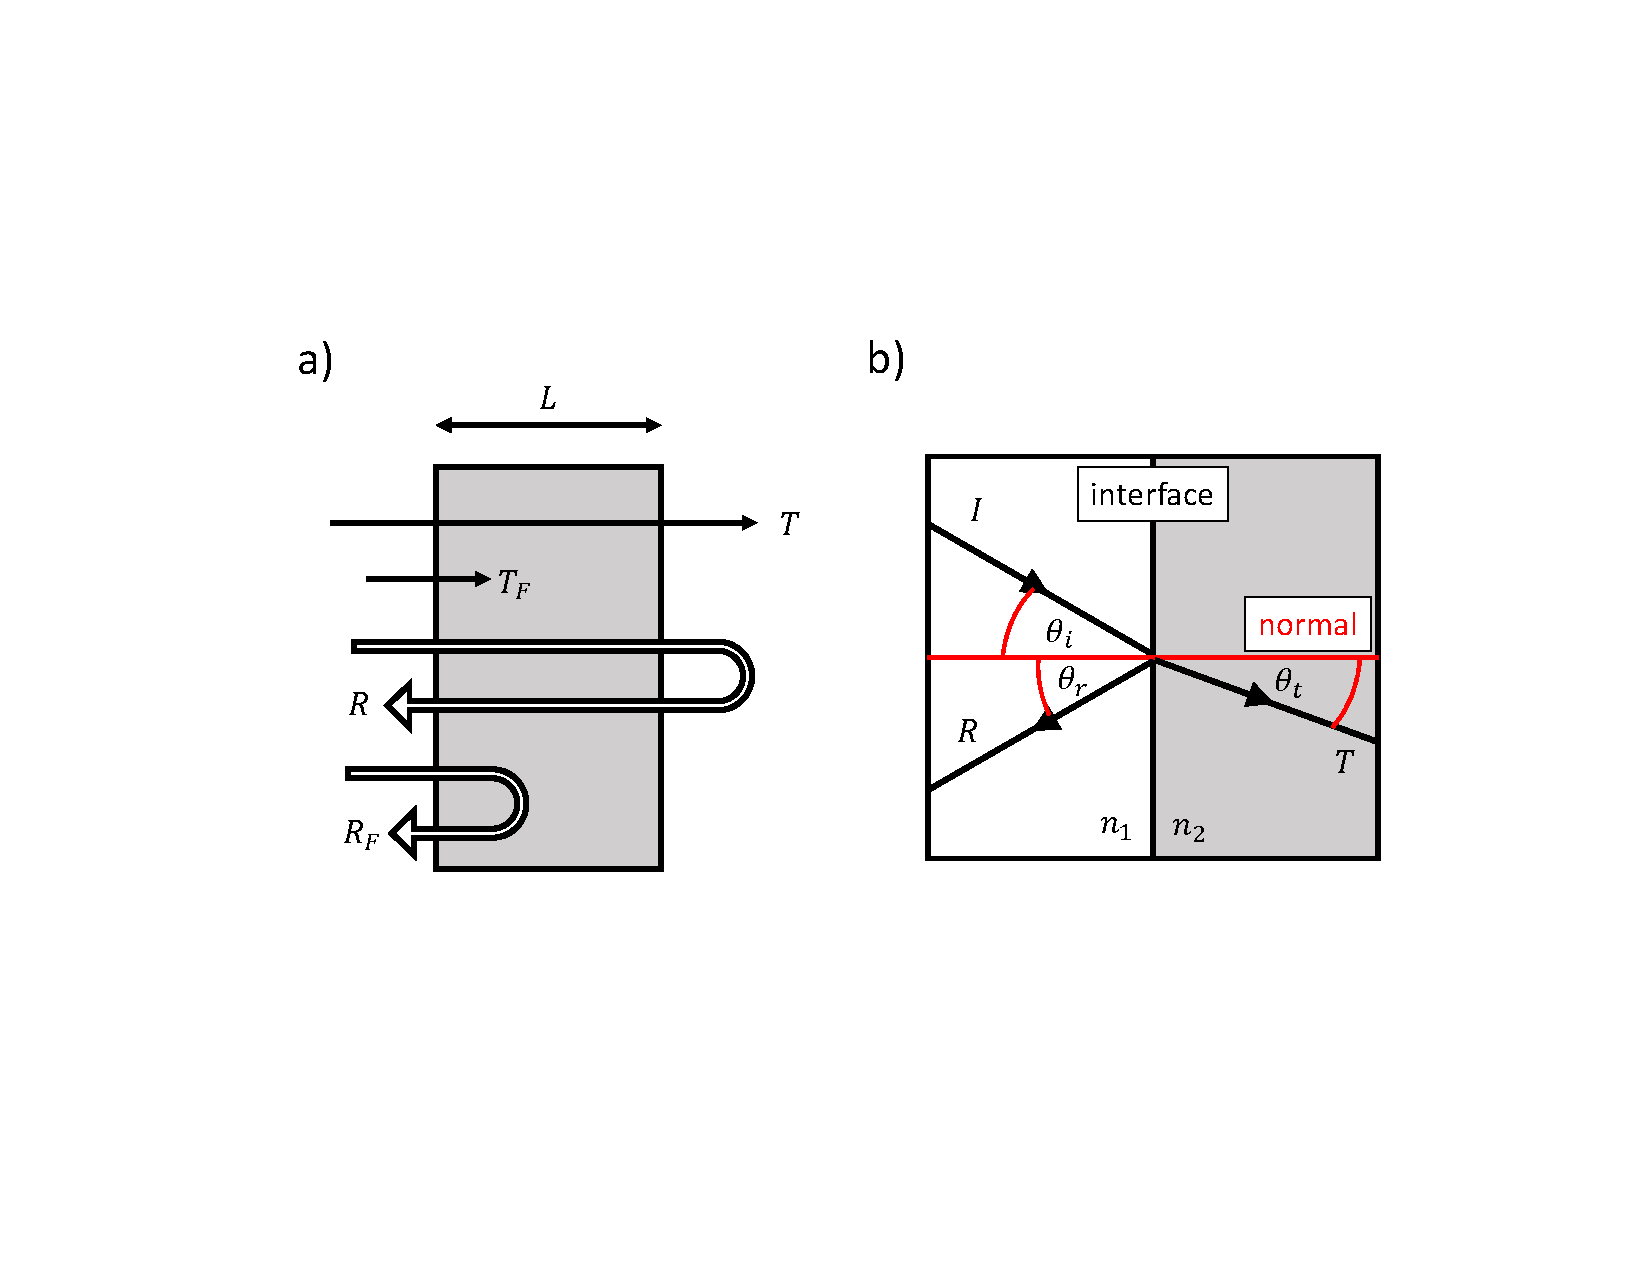
\includegraphics[width=0.75\textwidth]{figures/chap1/Fresnel_Geometry.pdf}
	\caption{Normal and non-normal incident geometries. \textbf{a)} Normal incidence geometry showing Fresnel coefficients $R_F$, $T_F$ for interfaces and total transmission $T$ and reflectance $R$ for a slab of thickness $L$. Figure recreated from \cite{nichelattiComplexRefractiveIndex2002}. \textbf{b)} Non-normal geometry showing definitions of angles $\theta_i, \theta_r$ and $\theta_t$ with respect to each interface.}
	\label{fig:Fresnel_Geometry}
\end{figure}

\begin{figure}
	\centering
	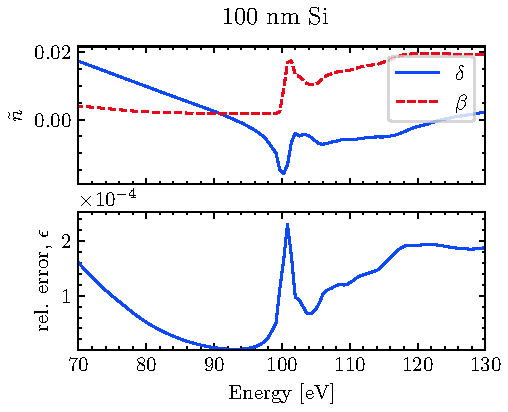
\includegraphics[width=0.75\textwidth]{figures/chap1/Si_transmission_Fresnel.pdf}
	\caption{Consequences of ignoring the real part of $\tilde{n}$ when calculating the transmission $T$ of a thin sample. Top panel: complex refractive index of silicon using the notation from \cref{eqn:complex_index}. The Si $L$-edge absorption feature is visible near 100 eV. Data from \cite{gulliksonCXROXRayInteractions}. Bottom panel: relative error in $T$, as defined in \cref{eqn:Fresnel_rel_err}, introduced by ignoring the contribution of $\Re(\tilde{n})$. An infinite number of bounces (e.g., \cref{eqn:Fresnel_coefs_inf_bounce}) is assumed.}
	\label{fig:Si_transmission_Fresnel}
	% plotted using \Python Scripts\CXRO\test\real_imag_index_plotting.py
\end{figure}

In a transient absorption experiment, we measure the transmission $T$ of a sample in response to excitation by an external field. Generally speaking, $T$ depends on both parts of the complex refractive index: $\tilde{n} = n + i k$. However, in a normal transmission geometry it turns out that the contribution of $\Im(\tilde{n})$ dominates the measured signal, and to a good approximation the role of $\Re(\tilde{n})$ can be ignored. Note that in a non-normal reflection geometry, both parts of $\tilde{n}$ make significant contributitions to the measured signal. In the following discussion we will analyze the Fresnel equations to see why this is the case. This section will draw from arguments made in reference \cite{nichelattiComplexRefractiveIndex2002}.

First, we consider the normal geometry shown in the left panel of \cref{fig:Fresnel_Geometry}. We write the complex index of refraction in the following form:
\begin{equation}
\begin{aligned}
\tilde{n} &= n - i k \\
&= (1-\delta) - i \beta
\end{aligned}
\label{eqn:complex_index}
\end{equation}
The Fresnel coefficients $R_F$ and $T_F$ describe the interface reflectance and transmittance and depend on both parts of the complex index $\tilde{n}$. For normal incidence, they are:
\begin{equation}
\begin{aligned}
R_F &= \left| \frac{n-ik-1}{n-ik+1}   \right|^2 \\
T_F &=  \frac{4n}{\left|n-ik+1\right|^2}
\end{aligned}
\label{eqn:fresnel_normal}
\end{equation}
Absorption in the bulk is described via the absorption length $\alpha$:
\begin{equation}
\alpha = 4 \pi k / \lambda
\end{equation}
Ignoring interface effects, the transmisison through the bulk is:
\begin{equation}
T_{\text{bulk}} = \exp( - \alpha L)
\end{equation}
Note that $\alpha$ and $T_{\text{bulk}}$ only depend on $k$.

The total reflectance $R$ and transmission $T$ are the result of interface effects plus bulk effects. We must consider the case where the detected light is the result of multiple reflections within the sample. Neglecting interference, we consider the case of $2N$ bounces where the laser's coherence length is less than the thickness of the bulk. In this case, the sum is incoherent with the expressions for $T$ and $R$ given by:
\begin{equation}
\begin{aligned}
R &= R_F + R_F T_F^2 T_{\text{bulk}}^2 \sum_{m=0}^{N} \left[ R_F T_{\text{bulk}} \right]^{2m} \\
T &= T_F^2 T_{\text{bulk}} \sum_{m=0}^{N} \left[ R_F T_{\text{bulk}} \right]^{2m}
\end{aligned}
\label{eqn:Fresnel_coefs_N_bounce}
\end{equation}
For the case of an infinite number of bounces, \cref{eqn:Fresnel_coefs_N_bounce} simplifies to:
\begin{equation}
\begin{aligned}
R &= R_F + \frac{R_F T_F^2 T_{\text{bulk}}^2}{1-R_F^2 T_{\text{bulk}}^2} \\
T &= \frac{T_F^2 T_{\text{bulk}}}{1-R_F^2 T_{\text{bulk}}^2},
\end{aligned}
\label{eqn:Fresnel_coefs_inf_bounce}
\end{equation}
whereas if only a single bounce occurs, \cref{eqn:Fresnel_coefs_N_bounce} reduces to:
\begin{equation}
\begin{aligned}
R &= R_F + R_F T_F^2 T_{\text{bulk}}^2 \\
T &= T_F^2 T_{\text{bulk}}
\end{aligned}
\label{eqn:Fresnel_coefs_1_bounce}
\end{equation}

We now consider the fractional error introduced by ignoring the interface effects described by $T_F$ and $R_F$. That is, what would happen if we assume that the interfaces have no effect on the transmitted intensity? We introduce the relative error $\epsilon$ made by ignoring the Fresnel coefficients of \cref{eqn:Fresnel_coefs_inf_bounce}:
\begin{equation}
\epsilon \equiv \frac{T_{\text{bulk}}}{T} - 1
\label{eqn:Fresnel_rel_err}
\end{equation}

As an example, consider a 100 nm thick Si sample measured in transmission near the Si $L$-edge (about 100 eV), as shown in \cref{fig:Si_transmission_Fresnel}. The relative error is in the range of one part in $10^4$ to $10^5$, well below our experimental detection limit. Silicon was chosen due to its data availability above and below the absorption edge, but this behavior should hold for all materials in normal transmission.

The real part of the complex index becomes important when the sample isn't normal to the beam, as shown in the right panel of \cref{fig:Fresnel_Geometry}. In this case, the Fresnel equations are a bit messier:
\begin{equation}
\begin{aligned}
R_s &= \left| \frac{\tilde{n}_1 \cos \theta_i - \tilde{n}_2 \cos \theta_t}{\tilde{n}_1 \cos \theta_i + \tilde{n}_2 \cos \theta_t}  \right|^2 \\
R_p &= \left| \frac{\tilde{n}_1 \cos \theta_t - \tilde{n}_2 \cos \theta_i}{\tilde{n}_1 \cos \theta_t + \tilde{n}_2 \cos \theta_i}  \right|^2 \\
T_s &= 1 - R_s \\
T_p &= 1 - R_p \\
%\theta_t &= \sqrt{1- \left( \frac{n_1}{n_2} \sin \theta_i \right)^2}
\end{aligned}
\label{eqn:Fresnel_nonnormal}
\end{equation}

Here, the subscripts $s$ and $p$ denote the polarization relative to the surface normal. For a sample in vacuum, $\tilde{n}_1=1$ and $\tilde{n}_2$ is the index of the sample. We can extract the relevant physics without any additional manipulation of \cref{eqn:Fresnel_nonnormal}. Right away, we can see that unlike \cref{eqn:fresnel_normal}, \cref{eqn:Fresnel_nonnormal} is symmetric in the real and imaginary parts of the sample's complex index, $\tilde{n}_2$. In the limit of a thick slab, ($L \gg \alpha$), the light is attenuated before it can reflect off the back surface and we have $T \rightarrow 0$ and $R \rightarrow R_{s,p}$. That is, the only contributions to the reflected intensity are from the interface and possibly the sample volume within $z \approx 1/\alpha$ of the interface. As a result, both parts of $\tilde{n}_2$ will make significant contributions to the reflected intensity. This geometry is common in transient reflection-absorption experiments \cite{cirriAchievingSurfaceSensitivity2017,kaplanFemtosecondTrackingCarrier2018}.



complex refractive index

sample requirements and preparation

pointing stability (in reflection, sample is an XUV optic)

\subsection{previous work}
what is state of the art?

previous work in condensed matter (Si, Ge, Si-Ge, etc)

motivation for long-wavelength studies in condensed matter

\subsection{physical observables in ATAS}
limited k-space information (requires single crystal)

transmission geometry measures imaginary and not the real part of n

\subsection{interpretation of experimental data}

\section{High Harmonic Generation}

High harmonic generation (HHG) is the extremely nonlinear process in which a strong infrared field produces light with frequencies that are integer multiples of the fundamental field after interacting with a medium. Rather than providing a first principles discussion of HHG, the main objective of this section is to understand how we can produce bright attosecond XUV light pulses with a sufficient spectral coverage for use in an ATAS experiment.

- spectral coverage of harmonics

- pulse duration of harmonic light

Gas phase HHG 

symmetry leads to odd harmonics.

gas and solid HHG has been studied

\subsection{Single Atom Response}

\begin{figure}
	\centering
	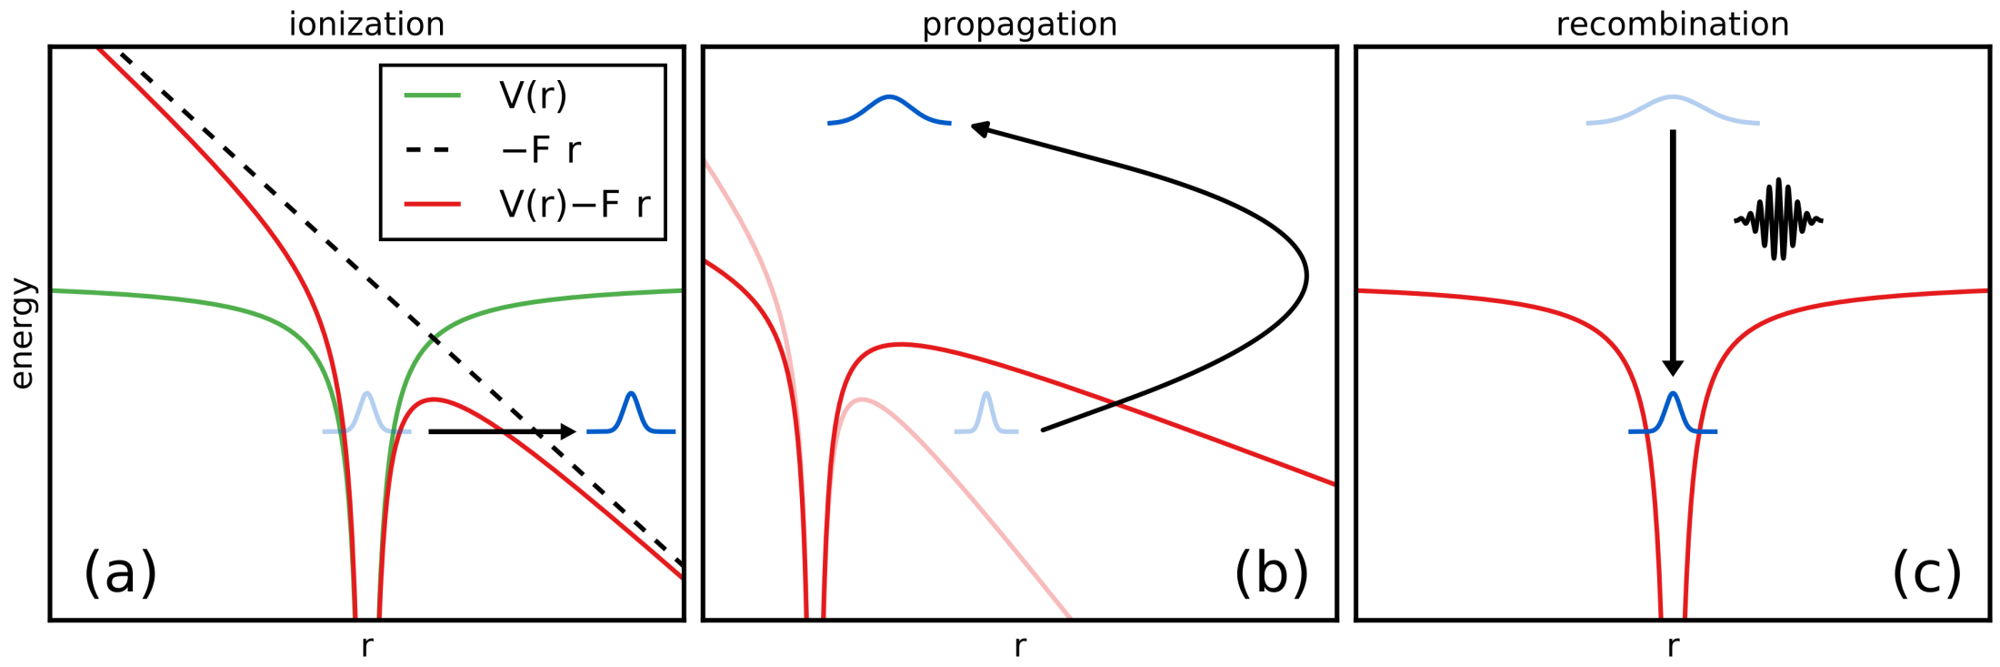
\includegraphics[width=0.75\textwidth]{figures/chap1/ThreeStepModel.png}
	\caption{The three step model of HHG. Figure adapted from \cite{schounAttosecondHighHarmonicSpectroscopy2015}.}
	\label{fig:ThreeStepModel}
\end{figure}

\begin{figure}
	\centering
	\subfloat[]{
		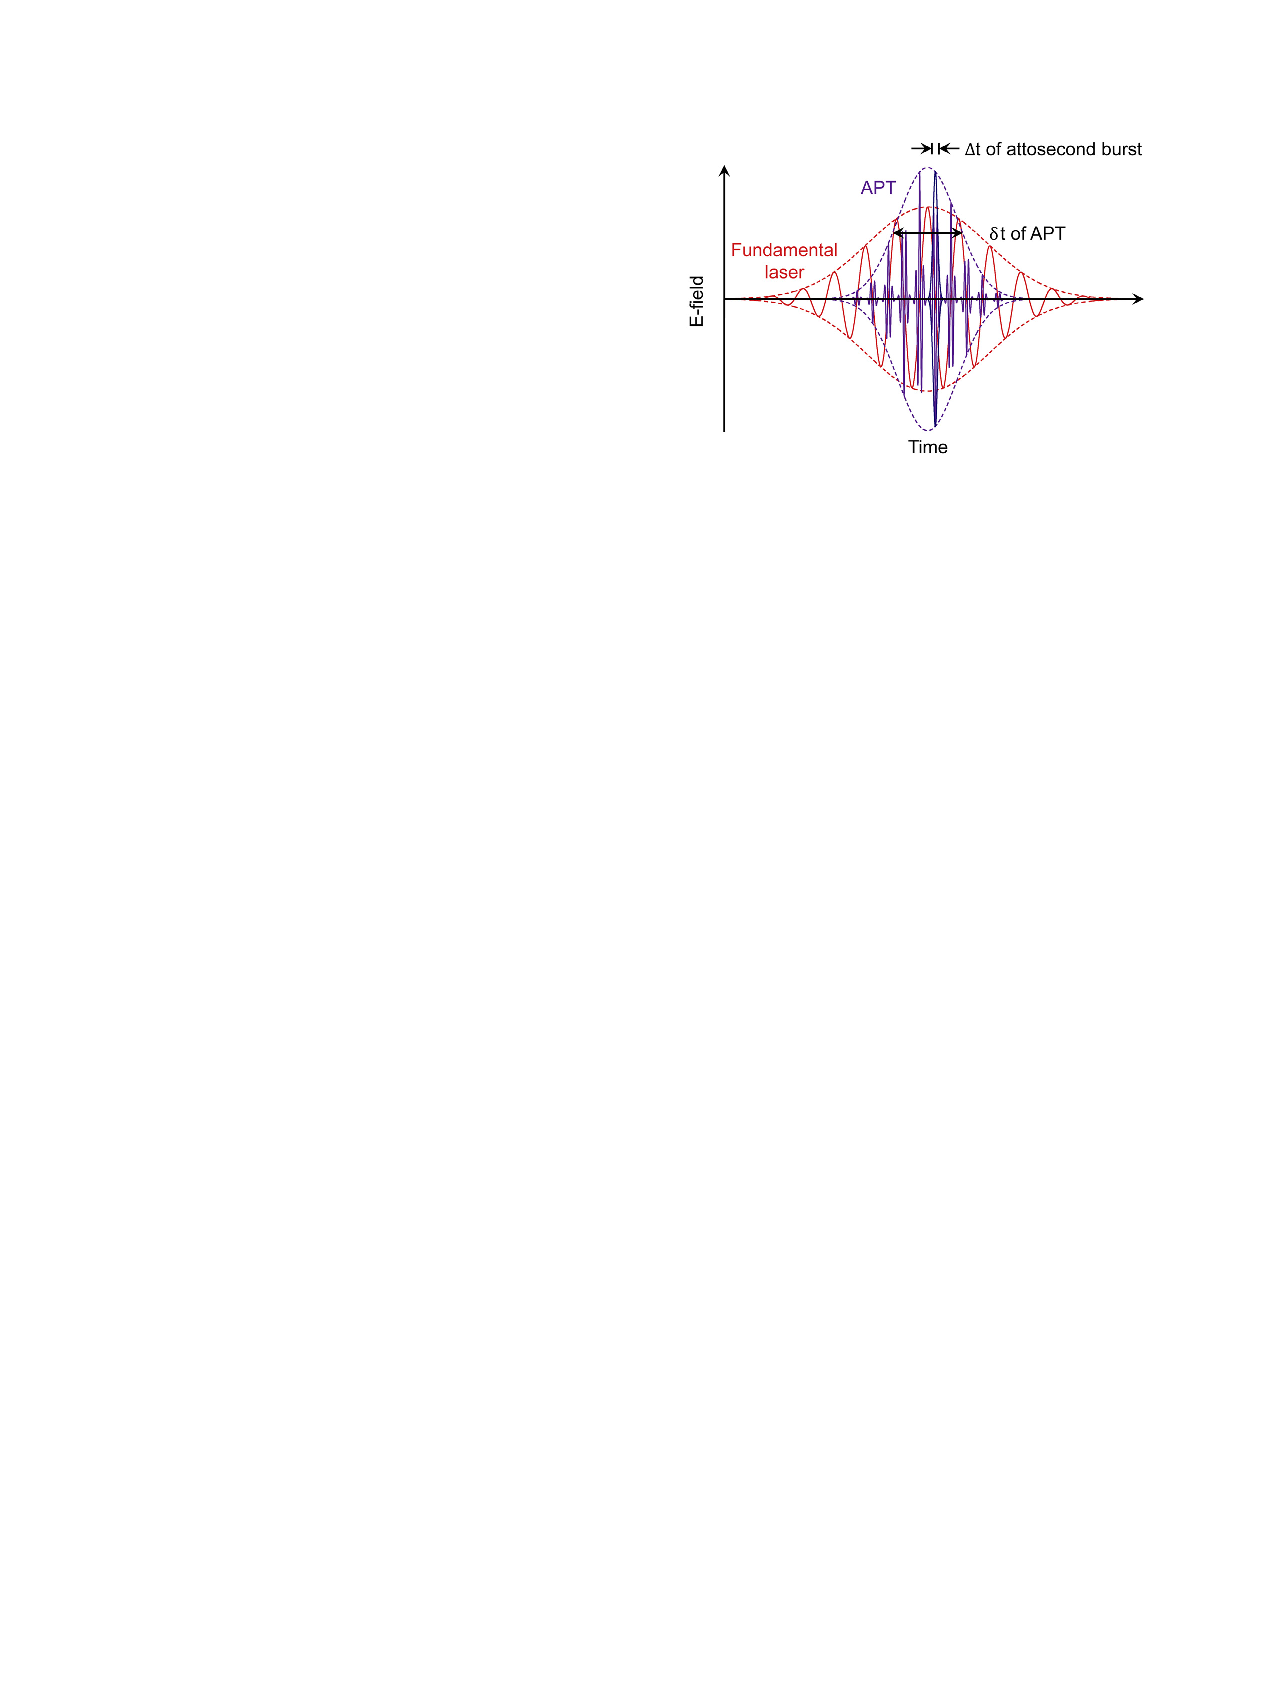
\includegraphics[width=0.4\textwidth]{figures/chap1/eich_APT_a.pdf}
		\label{fig:APT_time_domain}}
	\qquad
	\subfloat[]{
		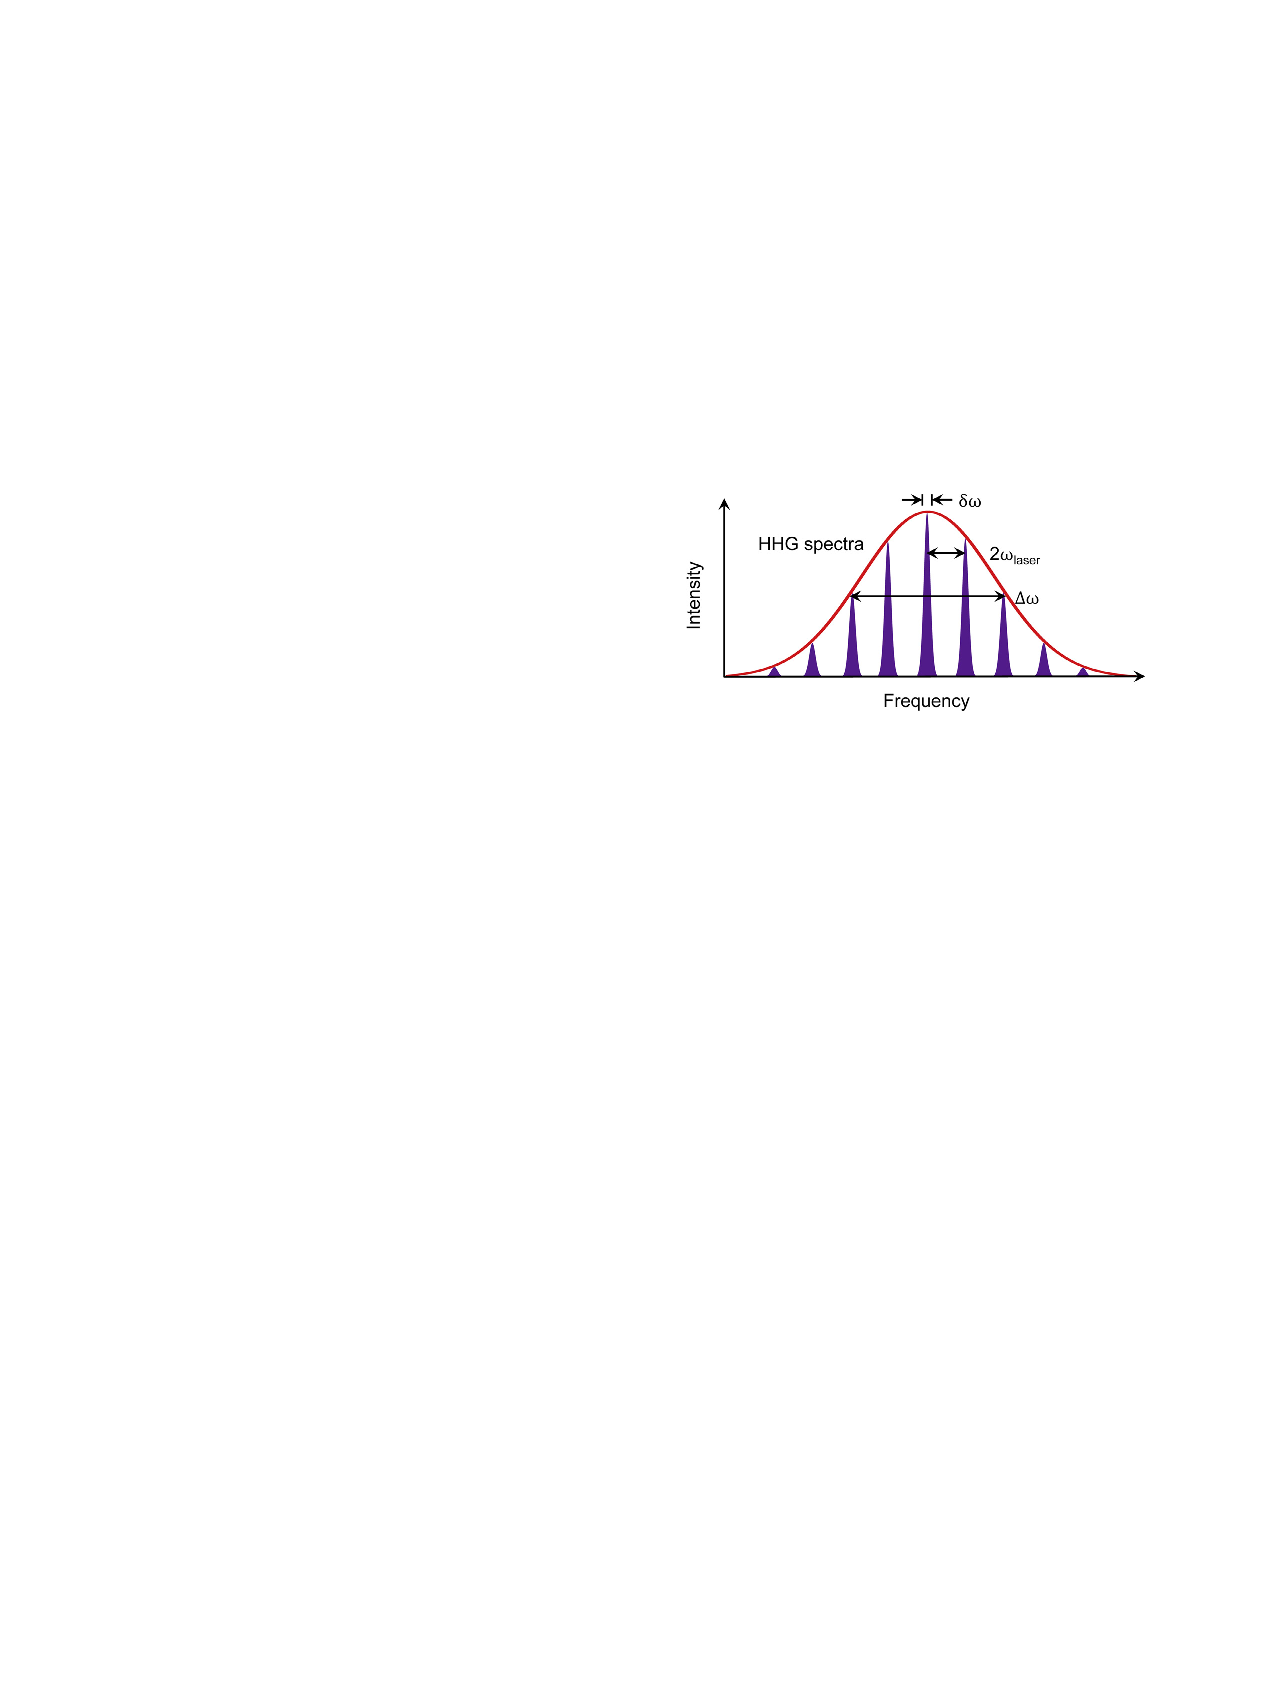
\includegraphics[width=0.4\textwidth]{figures/chap1/eich_APT_b.pdf}
		\label{fig:APT_freq_domain}}
	\caption{Time and frequency domain pictures of HHG. Figure adapted from \cite{eichTimeAngleresolvedPhotoemission2014}.}
	\label{fig:APT_IR_field}
\end{figure}

We start with a microscopic picture of harmonic generation, focusing on the interaction between a single atom and the laser field. In the early 1990s, a semi-classical model was developed to describe the process of high harmonic generation in three discrete steps: ionization, classical propagation in the vacuum, and recombination \cite{schaferThresholdIonizationHigh1993,corkumPlasmaPerspectiveStrong1993}. This model accurately predicts many of the fundamental features of HHG.

In the three step model, the electric field strength is on the order of the atomic potential that binds the electron to its parent atom. The valence electron's wavepacket evolves subject to the sum of the shielded Coloumb field and the spatially varying laser field. The electron can tunnel out of the distorted Coloumb field, as shown in the left panel of \cref{fig:ThreeStepModel}. This step is most likely to occur at the peak of the field, which occurs every half-cycle of the laser period.

The recently liberated electron is assumed to be born with zero initial kinetic energy. It accelerates in the oscillating laser field, gaining kinetic energy along the way, as shown in the central panel of \cref{fig:ThreeStepModel}. Its kinetic energy is proportional to the cycle-averaged quiver energy:
\begin{equation}
U_p = \frac{q_e^2 F_0^2}{4 m_e \omega^2} \propto I_0 \lambda^2
\label{eqn:Up}
\end{equation}
where $m_e$ is the electron mass, $q_e$ is the electron charge, $\omega$ is the frequency, $F_0$ is the electric field strength, $I_0$ is the intensity, and $\lambda$ is the wavelength of the laser. A more useful form of \cref{eqn:Up} is given below:
\begin{equation}
U_p \textrm{ [eV]} = \left( 9.33738 \times 10^{-5} \right) \times I_0 \textrm{[PW/cm\textsuperscript{2}]} \times \lambda\textrm{[nm]}^2
\end{equation}

The birth phase of the electron (relative to the laser period) determines its classical trajectory. Some electrons will be driven away from the parent ion, never to return; some will be driven back to the birth location, where they can scatter off of, miss, or recombine with the parent ion. We will only concern ourselves with those electrons that recombine (right panel of \cref{fig:ThreeStepModel}). Upon recombination, the electron will emit a photon of energy $I_p + KE$, where $I_p$ is the ionization potential of the atom and $KE$ is the kinetic energy acquired during the propagation step. A classical analysis of the electron propagation reveals that the maximum kinetic energy such an electron can gain is $3.17 U_p$, and therefore the maximum photon energy is: 
\begin{equation}
\hbar \omega_{cutoff} = I_p + 3.17 U_p
\label{eqn:cutoff_energy}
\end{equation}
This quantity is often called the cutoff energy, and it is proportional to $I_0 \lambda^2$. Thus, we can extend the maximum photon energy of the harmonics by increasing the fundamental wavelength of the laser.

Unfortunately, the brightness of an individual harmonic order will decrease strongly with increasing wavelength, with the intensity scaling between $\lambda^{-5}$ and $\lambda^{-6}$ \cite{tateScalingWavePacketDynamics2007,shinerWavelengthScalingHigh2009}. We can conceptually understand this as the compounding of two separate problems \cite{lewensteinTheoryHighharmonicGeneration1994}. First, longer wavelengths extend the cutoff energy, spreading a fixed harmonic conversion efficiency across more harmonics and lowering the brightness of each individual harmonic. This accounts for a factor of $\lambda^{-2}$. Secondly, the recombination probability scales inversely with square of the electron wavepacket spread that occurs during the propagation step. Longer wavelengths mean longer excursion times $\tau$, and the wavepacket spreads out as $\tau^{3/2}$. Since we are concerned with the harmonic intensity, we square this value to get $\tau^3 \propto \lambda^{-3}$. With this simple argument, we can see why the harmonic brightness should decrease as $\lambda^{-5}$.

So far, it appears that XUV spectrum is continuous in energy, ranging from $I_p$ to $\hbar \omega_{cutoff}$. This is because we have been considering the effects of a single-cycle laser pulse. In a multi-cycle pulse, the ionization-propagation-recombination steps will happen twice per pulse (every $T_0/2$ seconds), and each event results in a brief burst of light, as shown in \cref{fig:APT_time_domain}. If we Fourier transform this comb of attosecond pulses, we will get a comb in the frequency domain with separation $2 \omega_0$, as shown in \cref{fig:APT_freq_domain}. Thus, we expect to see only odd harmonics of the laser frequency $\omega_0$.

\subsection{Macroscopic Picture}

We now zoom out to the macroscopic picture, which encompasses the entire gas-laser interaction volume. In the far field, the radiation from individual atoms will be coherently summed to form an bright XUV light source. The overall efficiency of the HHG process depends on the phase mismatch $\Delta k$ of the individual dipoles across the interaction volume. We will see how the phase matching determines optimal interaction pressures for a given driving wavelength. Additionally, we will see the effect of XUV reabsorption by the gas on the overall XUV brightness.

\subsubsection{Phase Matching}

HHG will be an efficient process if the wave vector mismatch $\Delta k$ of the independent dipoles is zero. The phase mismatch term can be expressed as three separate factors, each arising from distinct physical phenomena \cite{rothhardtAbsorptionlimitedPhasematchedHigh2014}:
\begin{equation}
\Delta k = \Delta k_{disp} + \Delta k_{Gouy} + \Delta k_{dipole}
\label{eqn:phase_mismatch}
\end{equation}
The first term represents the dispersion from the generating medium. It has contributions from both the neutral atoms and the free electrons:
\begin{equation}
\Delta k_{disp} = \frac{2 \pi q}{\lambda} \frac{p}{p_0} \Delta \delta \left( 1 - \frac{\eta}{\eta_c} \right)
\end{equation}
Here, $q$ is the harmonic order, $\Delta \delta$ is the difference of the refractive indices of the fundamental and high order harmonic, $p_0$ is the standard pressure (1013 mbar), $p$ is the interaction pressure, $\eta$ is the ionization fraction and $\eta_c$ is the critical ionization fraction (the fraction at which the plasma dispersion of the free electrons exceeds the atomic dispersion).

The second term is the geometrical phase mismatch caused by focusing:
\begin{equation}
\Delta k_{Gouy} = q \pdv{\varphi_{Gouy}}{z} = q \pdv{z} \left( - \arctan \left( \frac{z}{z_R} \right) \right)
\label{eqn:deltak_Gouy}
\end{equation}
Here, $z_R = \pi w_0^2 / \lambda$ is the Rayleigh range and $z=0$ corresponds to the focal plane. Note that $\Delta k_{Gouy}$ is negative for all values of $z$. The atomic term arises from the intensity-dependent dipole phase acquired during the electron excursion \cite{lewensteinTheoryHighharmonicGeneration1994,balcouGeneralizedPhasematchingConditions1997,salieresCoherenceControlHighOrder1995}:
\begin{equation}
\Delta k_{dipole} = - \alpha_q \pdv{I}{z}
\label{eqn:deltak_atomic}
\end{equation}
The value of $\alpha_q$ depends on the quantum trajectory the electron takes during its excursion. For short trajectories, {$\alpha_q = 2 \times 10^{-14}$ cm\textsuperscript{2}/W} and for long trajectories, {$\alpha_q = 22 \times 10^{-14}$ cm\textsuperscript{2}/W} \cite{kazamiasPressureinducedPhaseMatching2011,balcouQuantumpathAnalysisPhase1999}. The sign of $\Delta k_{dipole}$ is positive (negative) if the gas source is located upstream (downstream) of the focus.

Experimentally, the phase matching can be adjusted by tuning the laser parameters (wavelength $\lambda$, intensity $I$, pulse duration, focal spot size $w_0$), the gas species ($I_p, n$ and $k$) and interaction pressure $P$, and the gas location relative to the laser focus ($z$). Additionally, a variable aperture (iris) located just before the generation lens effectively tunes multiple laser parameters simultaneously, and is known colloquially as ``the magic iris trick" \cite{kazamiasHighOrderHarmonic2002}. Because $\Delta k$ is dependent on the harmonic order $q$, it is impossible to perfectly phase match the entire harmonic spectrum simultaneously. As a result, we adjust the phase matching parameters to optimize the useful part of the harmonic spectrum, usually at the expense of the rest of the spectrum.

Also note that the dispersion phase can be controlled by tuning the interaction pressure $p$, while the other terms are (to first order) pressure independent. If the gas medium is at focus, $\pdv{I}{z} = 0$ and therefore $k_{dipole}=0$. In this case, the condition $\Delta k = 0$ can be met by setting to the pressure to an optimal phase matching pressure $p_{opt}$ \cite{rothhardtAbsorptionlimitedPhasematchedHigh2014}:
\begin{equation}
p_{opt} = p_0 \frac{\lambda^2}{2 \pi^2 w_0^2 \Delta \delta \left( 1 - \frac{\eta}{\eta_c} \right)}
\label{eqn:phase_matching_pressure}
\end{equation}

We therefore arrive at the conclusion that the optimal phase matching pressure scales with the square of the fundamental wavelength. Furthermore, tighter focusing ($w_0 \rightarrow 0$) and higher ionization fractions ($\eta \rightarrow \eta_c$) require larger pressures. Therefore, creating bright harmonics from a long wavelength, relatively weak pulse requires significantly higher interaction pressures than a strong 800 nm pulse. This is the motivation for designing a vacuum system and gas source that can deliver high interaction pressures.

\subsubsection{XUV Reabsorption}
\label{sec:XUV_reabsorption}

\begin{figure}
	\centering
	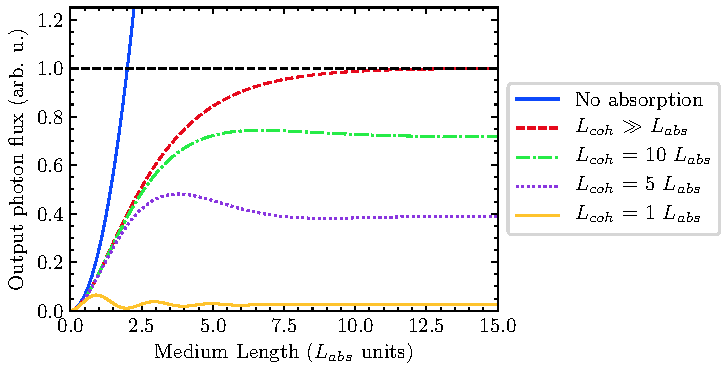
\includegraphics[width=0.75\textwidth]{figures/chap1/Constant1999_fig1.pdf}
	\caption{1D absorption model from \cref{eqn:HHG_Nout_simple}.}
	\label{fig:Constant1999_fig1}
	% created with \Python Scripts\HHG_Phasematching-master\test\Constant_fig1.py
\end{figure}

We now consider the effects of XUV absorption on the phase matching process using the 1-dimension model introduced by Constant et. al. \cite{constantOptimizingHighHarmonic1999}. In doing so, we restrict ourselves to the on-axis emission of the $q$\textsuperscript{th} harmonic. That is, we consider only harmonics with a wave vector $k_q$ that is collinear to the fundamental ($k_0$). In this case, the number of photons emitted per unit time and area is:
\begin{equation}
N_{out} = \frac{\omega_q}{4 c \epsilon_0 \hbar} \left| \left[ \int_{0}^{L_{med}} \dd{z} \rho(z) A_q(z) \exp \left( - \frac{L_{med} - z}{2 L_{abs}}  \right) \exp \left( i \varphi_q(z) \right)  \right] \right|^2
\label{eqn:HHG_Nout}
\end{equation}
Here, $\rho(z)$ is the gas medium density, $A_q(z)$ is the amplitude of the harmonic response at frequency $\omega_q$ and $\varphi_q$ is its phase at the exit of the medium, which has length $L_{med}$. If we are using a loose focusing geometry, then the gas density and harmonic response amplitude are constant along the interaction volume: $\rho(z) = \rho$ and $A_q(z)=A_q$. With this restriction, \cref{eqn:HHG_Nout} evaluates to:
\begin{equation}
\begin{aligned}
N_{out} = & \\ \rho^2 A_q^2 & \frac{4L_{abs}^2}{1+4\pi^2(L_{abs}^2 / L_{coh}^2)} \left[ 1 + \exp\left(-\frac{L_{med}}{L_{abs}}\right) - 2 \exp\left(\frac{\pi L_{med}}{L_{coh}}\right) \exp\left(-\frac{L_{med}}{2L_{abs}}\right) \right]
\label{eqn:HHG_Nout_simple}
\end{aligned}
\end{equation}
Here, we use the notation $L_{coh} = \pi/\Delta k$ for the coherence length ($\Delta k = k_q - q k_0$) and $L_{abs} = 1/{\sigma \rho}$ for the absorption length.


\cref{eqn:HHG_Nout_simple} is plotted in \cref{fig:Constant1999_fig1}. In the case of no absorption ($L_{abs} \rightarrow \infty$), the harmonic yield grows as $L_{med}^2$. Otherwise, the optimized conditions are $L_{med} > 3 L_{abs}$ and $L_{coh} > 5 L_{abs}$.

Experimentally, $L_{med}$ is fixed by the geometry of the gas source, $L_{abs}$ is directly controlled by adjusting the backing pressure, and $L_{coh}$ is indirectly controlled by other parameters (gas source position relative to focus, focusing conditions, iris diameter, etc.). In \cref{sec:HHG_gas_sources}, we will apply this simple model to the gas sources available in our lab to maximize our HHG yield.

\textbf{to do:}

now, find out where you are on this plot for the different gas cell geometries. that is, free jet, LPC and HPC have set medium lengths. given their pressure performance, you can calculate the range of interaction pressures achievable by each HHG source, and therefore you can calculate the Labs for a specific generating gas (Ar, for example). having done that, you know the Labs and the Lmed, so you know the x-axis position. you still don't know the coherence length, but it's a start.

motivation: in the LPC, we can't see pressure rollover. this plot helps show why. (assuming the LPC and the free jet are still on the rising edge of the curves). this plot explains why.

\chapter{ANITA instrument}
\label{anita}

\section{ANITA payload}
\label{payload}

The {\bf AN}tarctic {\bf I}mpulsive {\bf T}ransient {\bf A}ntenna (\gls{anita}) is a NASA-sponsored long-duration balloon experiment with the primary goal of detecting \gls{uhe} neutrinos as broadband radio signals in the frequency range $200 - 1200\,\mbox{MHz}$. The \gls{anita}-4 payload at the NASA \gls{ldb} Facility is shown in Figure~\ref{my_anita}. The \gls{anita}-4 payload just prior to launch and after launch at its float altitude through a telescope is shown in Figures~\ref{balloon_filled} and ~\ref{launch_float}.
The most important parts of the \gls{anita} payload are its \gls{rf} antennas and its signal processing units (most of which are inside the Instrument Box). A peer-reviewed description of these can be found in a recent publication that I led as the corresponding author~\cite{tuff}. \href{https://www.sciencedirect.com/science/article/pii/S016890021830411X}{Click here to find the electronic version of this paper.} 

\begin{figure}
\centering
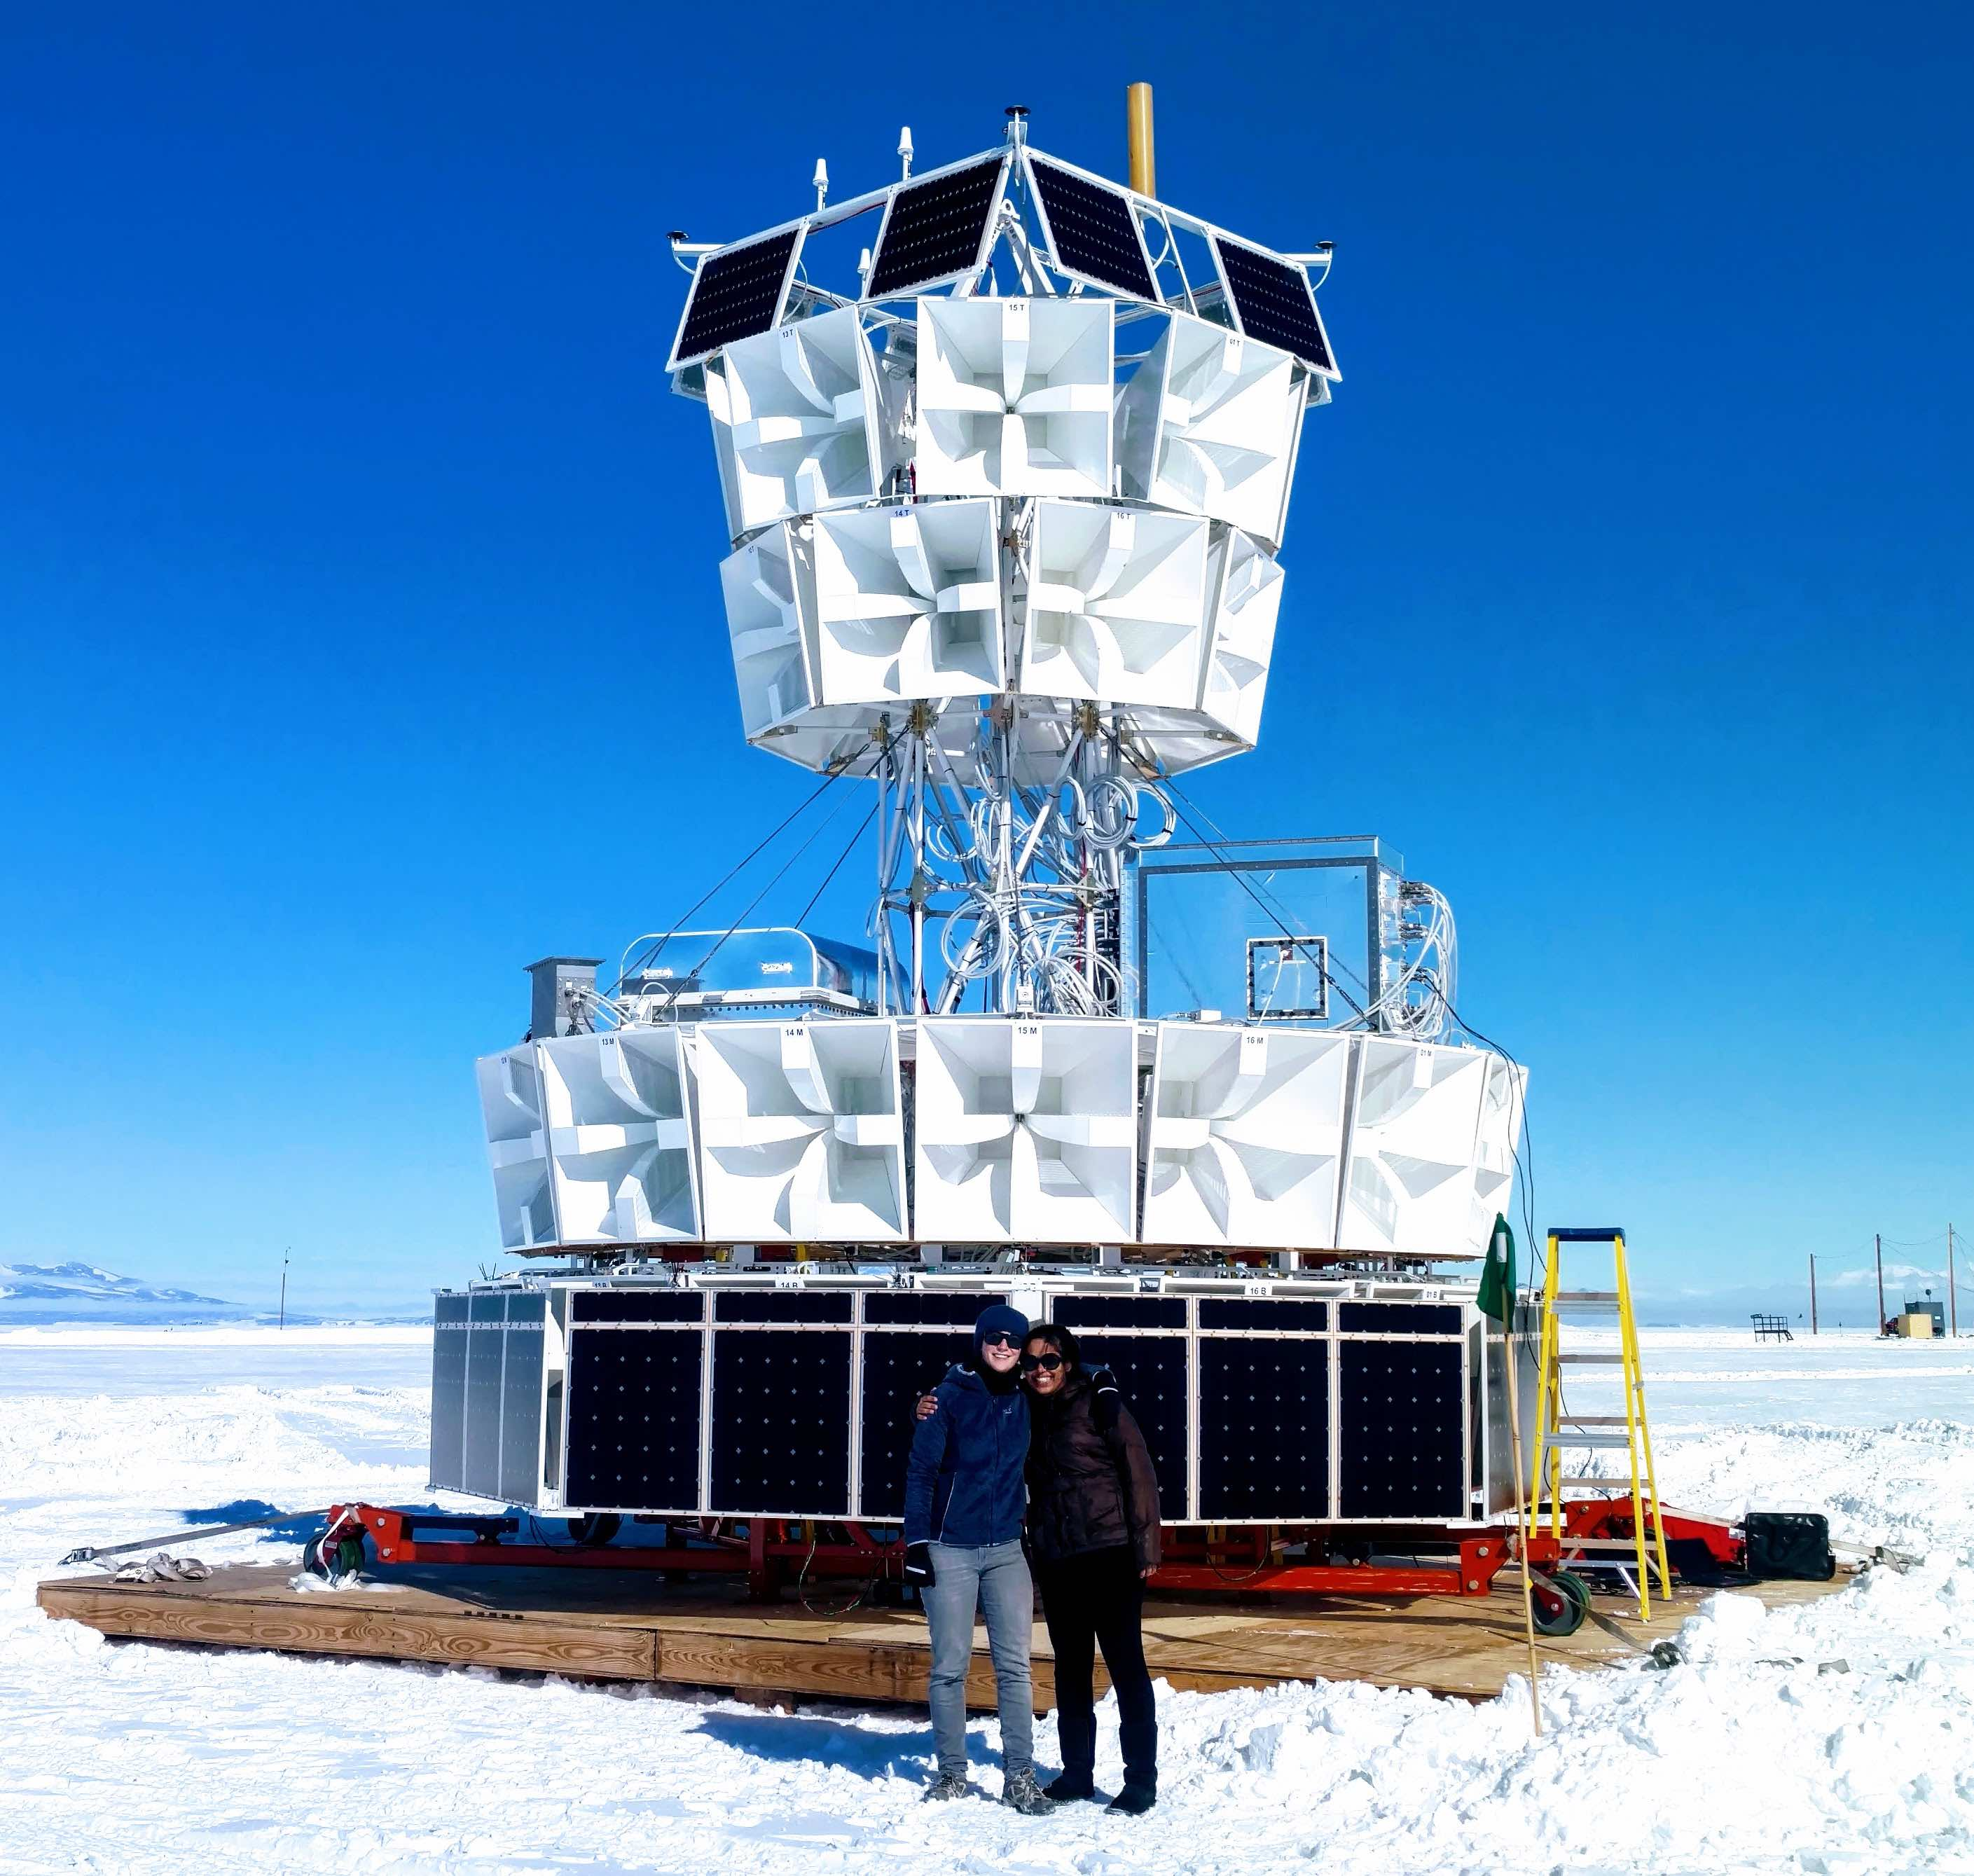
\includegraphics[width=1.0\textwidth]{figures/anita_thesis.jpg}
\caption{Linda Cremonesi and I during testing the GPS systems on ANITA-4 before its launch from near McMurdo Station, Antarctica. This shows the relative size of the instrument compared to humans. Picture credit: Steven Prohira.}
\label{my_anita}
\end{figure}

\begin{figure}
\centering
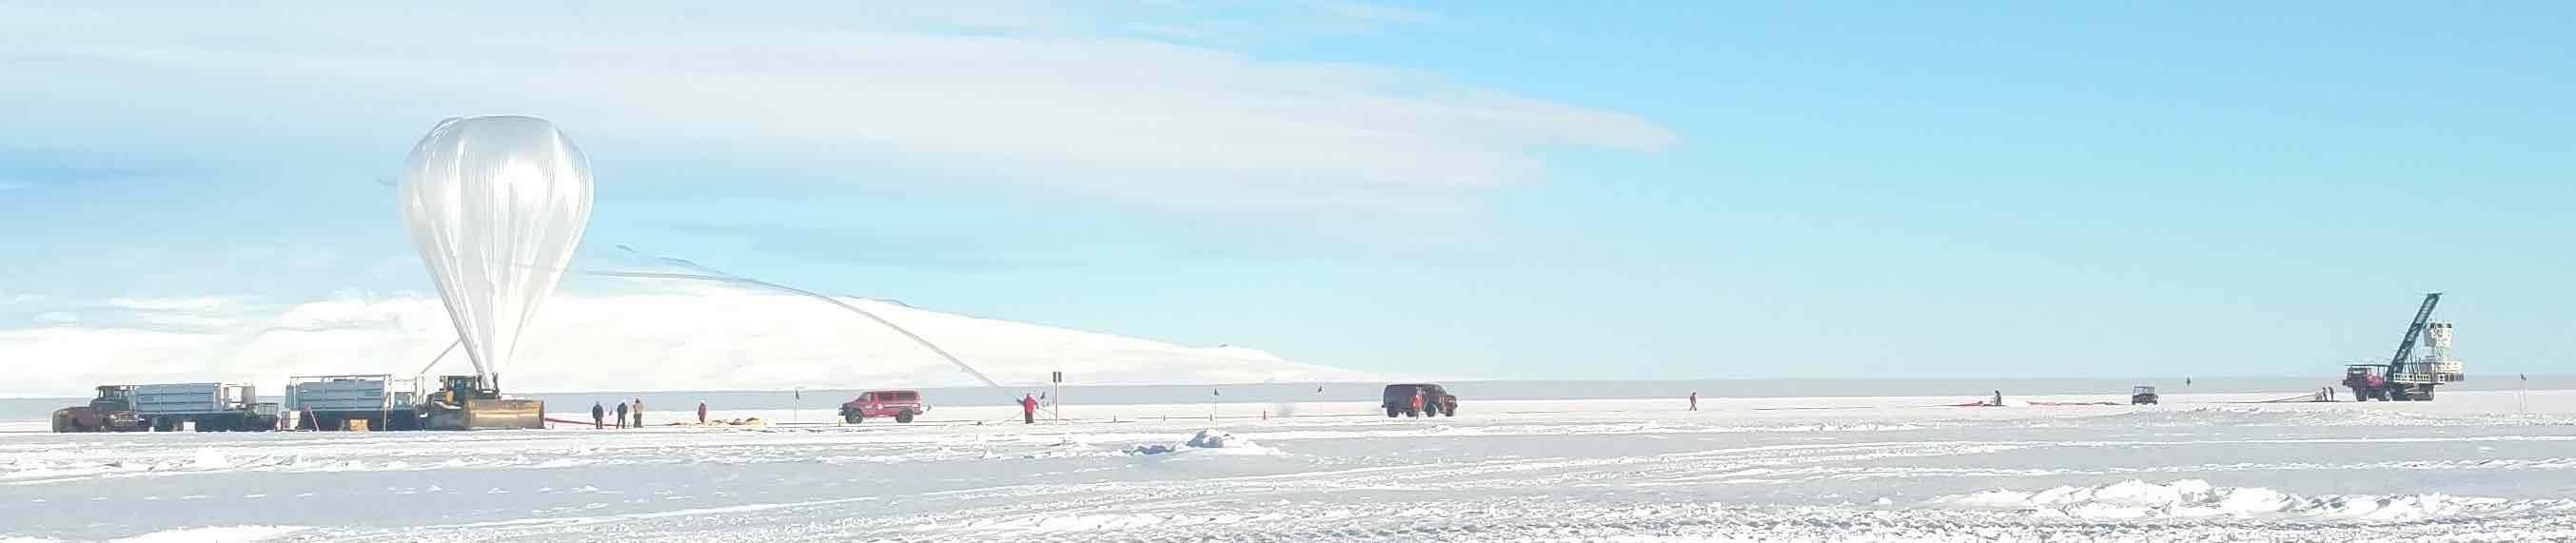
\includegraphics[width=1.0\textwidth]
{figures/launch_balloon.jpg}
\caption{Here NASA's balloon for the launch of ANITA-4 is being filled with Helium. When NASA takes the balloon out, one knows there will be a launch for real.}
\label{balloon_filled}
\end{figure}

\begin{figure}
\centering
\subfloat[ANITA-4 at launch]{
	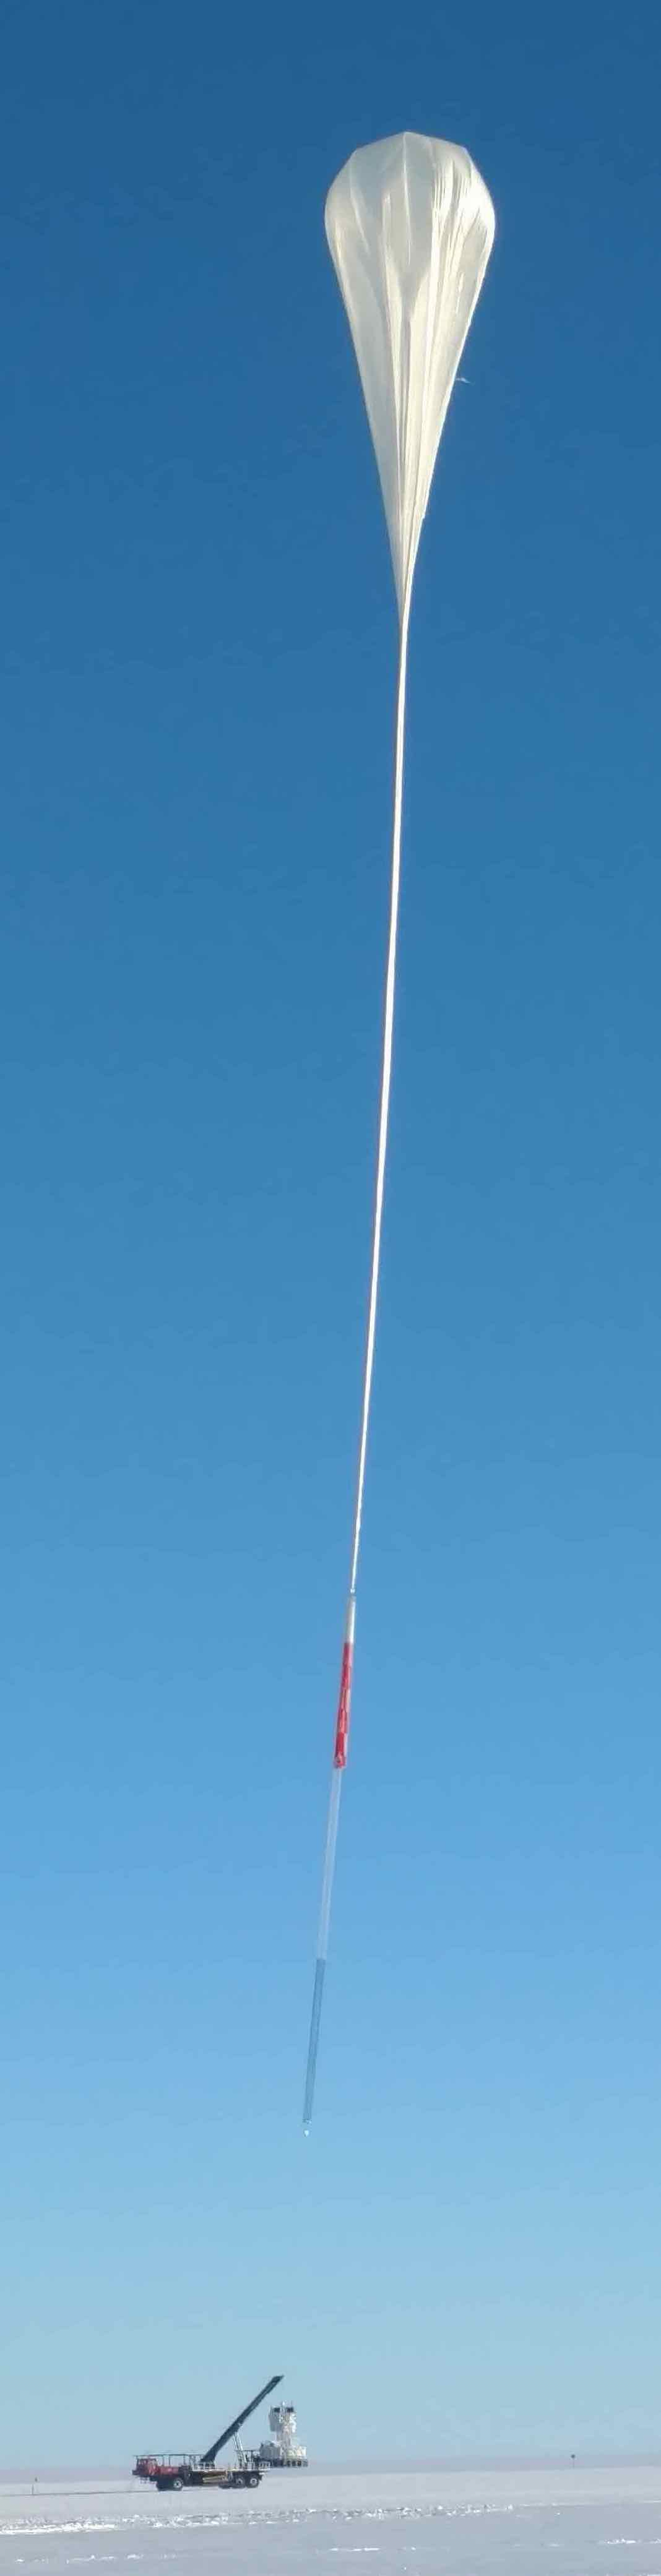
\includegraphics[width=0.24\textwidth]
	{figures/launch_thesis.jpg}
	\label{launch}
}
\subfloat[ANITA-4 at float altitude]{
	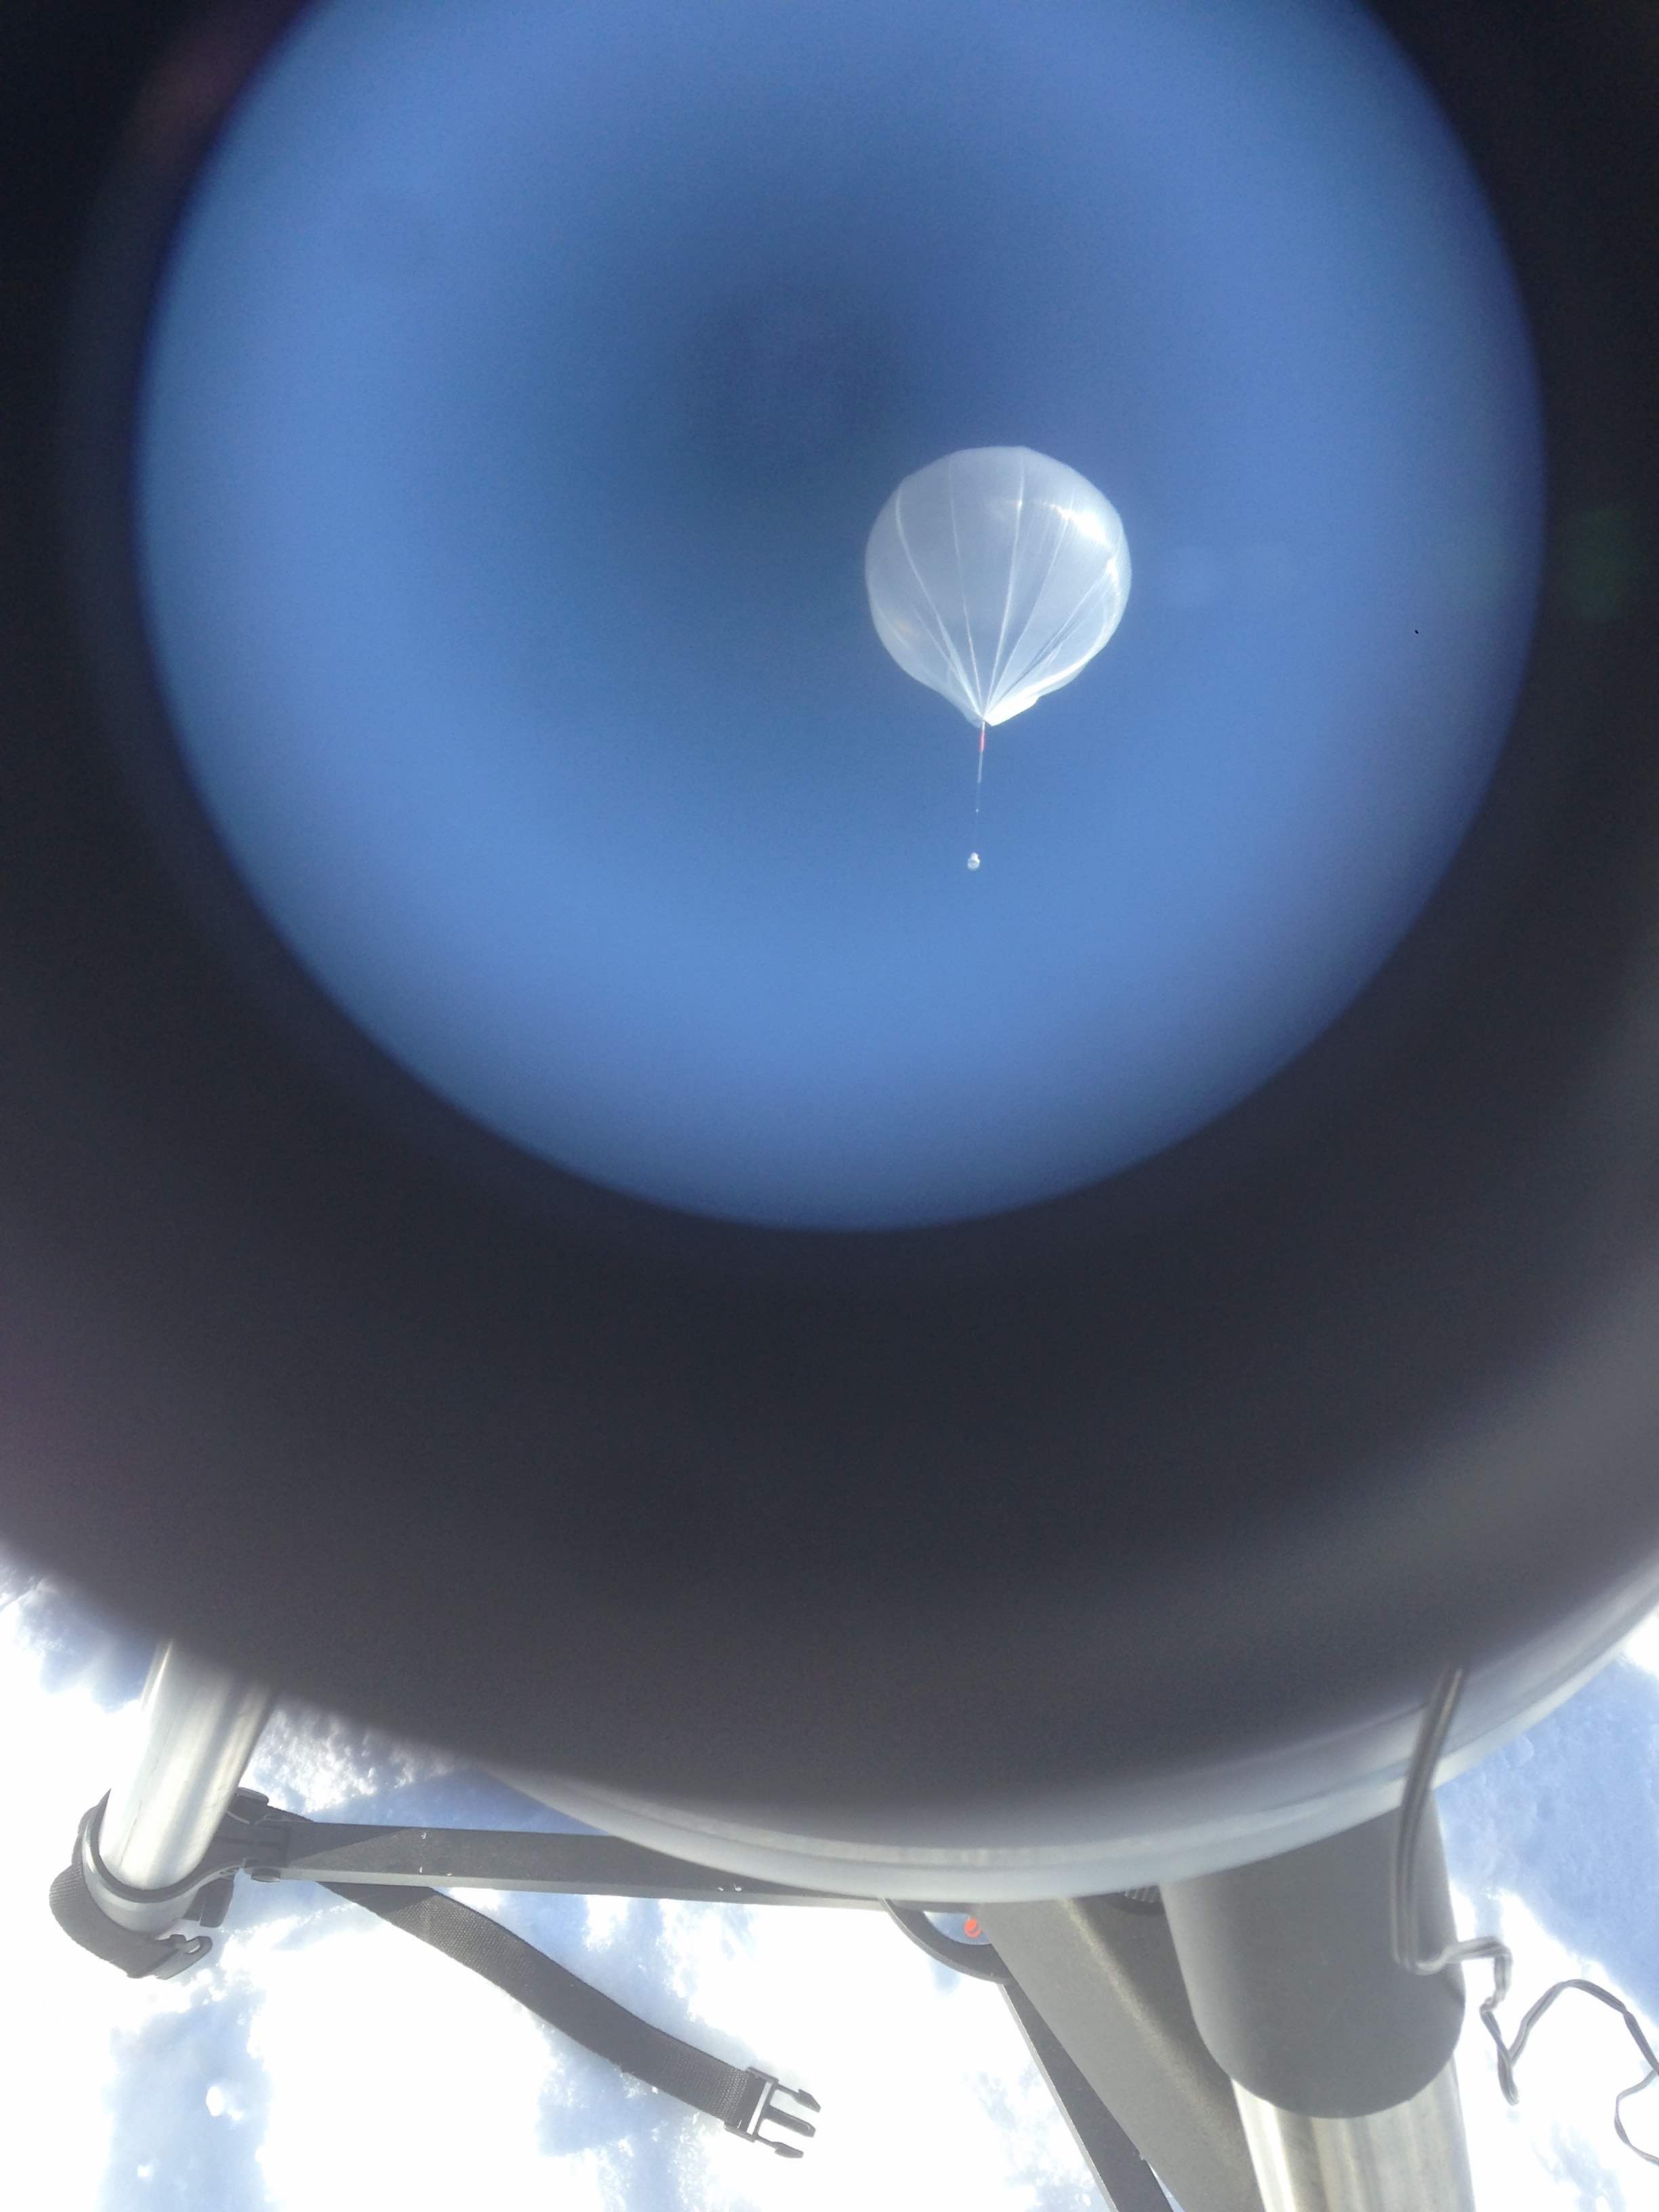
\includegraphics[width=0.7\textwidth]
	{figures/anita_float_big.jpg}
	\label{anita_float_big}
}
\caption{Left: The ANITA-4 payload attached to its balloon just before launch. Right: When ANITA gets close to its float altitude of about $40$ km, one cannot see it from the ground with the naked eye. This is ANITA-4 through a telescope. Telescope picture credit: Steven Prohira.}
\label{launch_float}
\end{figure}

\subsection{Flight path and payload weight}

The \gls{anita} neutrino observatory is a NASA long-duration balloon-borne payload.
After its launch from the NASA \gls{ldb} Facility near McMurdo Station,
the Summer polar vortex winds keep the ANITA payload flying in roughly circular loops above the continent of Antarctica. 
A lighter payload is able to reach higher altitudes where the polar vortex is spatially tighter. 
This leads to a more favorable flight path which, in turn, increases the chances of a longer flight and increased livetime. 
Most importantly, this 
keeps the payload from 
venturing out over the ocean and becoming unrecoverable. 

There are strict weight restrictions on a balloon payload. 
This is why
the \gls{anita} gondola is made of hollow aluminum tubes connected by joints. 
The aluminum beams can be seen in Figure~\ref{hanging}. 
A need for a light payload informed the design of the \gls{tuff} boards as detailed
in Section~\ref{tuff}. 
This helps to keep the payload weight under $5000\,\mbox{lb}$. 
The ANITA-4 payload weighed $4526\,\mbox{lb}$. 
For the first time, the \gls{anita}-4 payload was able to reach above $40\,\mbox{km}$ altitude for part of its flight. 
Furthermore, the ANITA-4 payload was able to maintain a more favorable flight path compared to the \gls{anita}-3 payload, resulting in a longer flight of 27 days compared to 22 days in \gls{anita}-3.

\begin{figure}
\centering
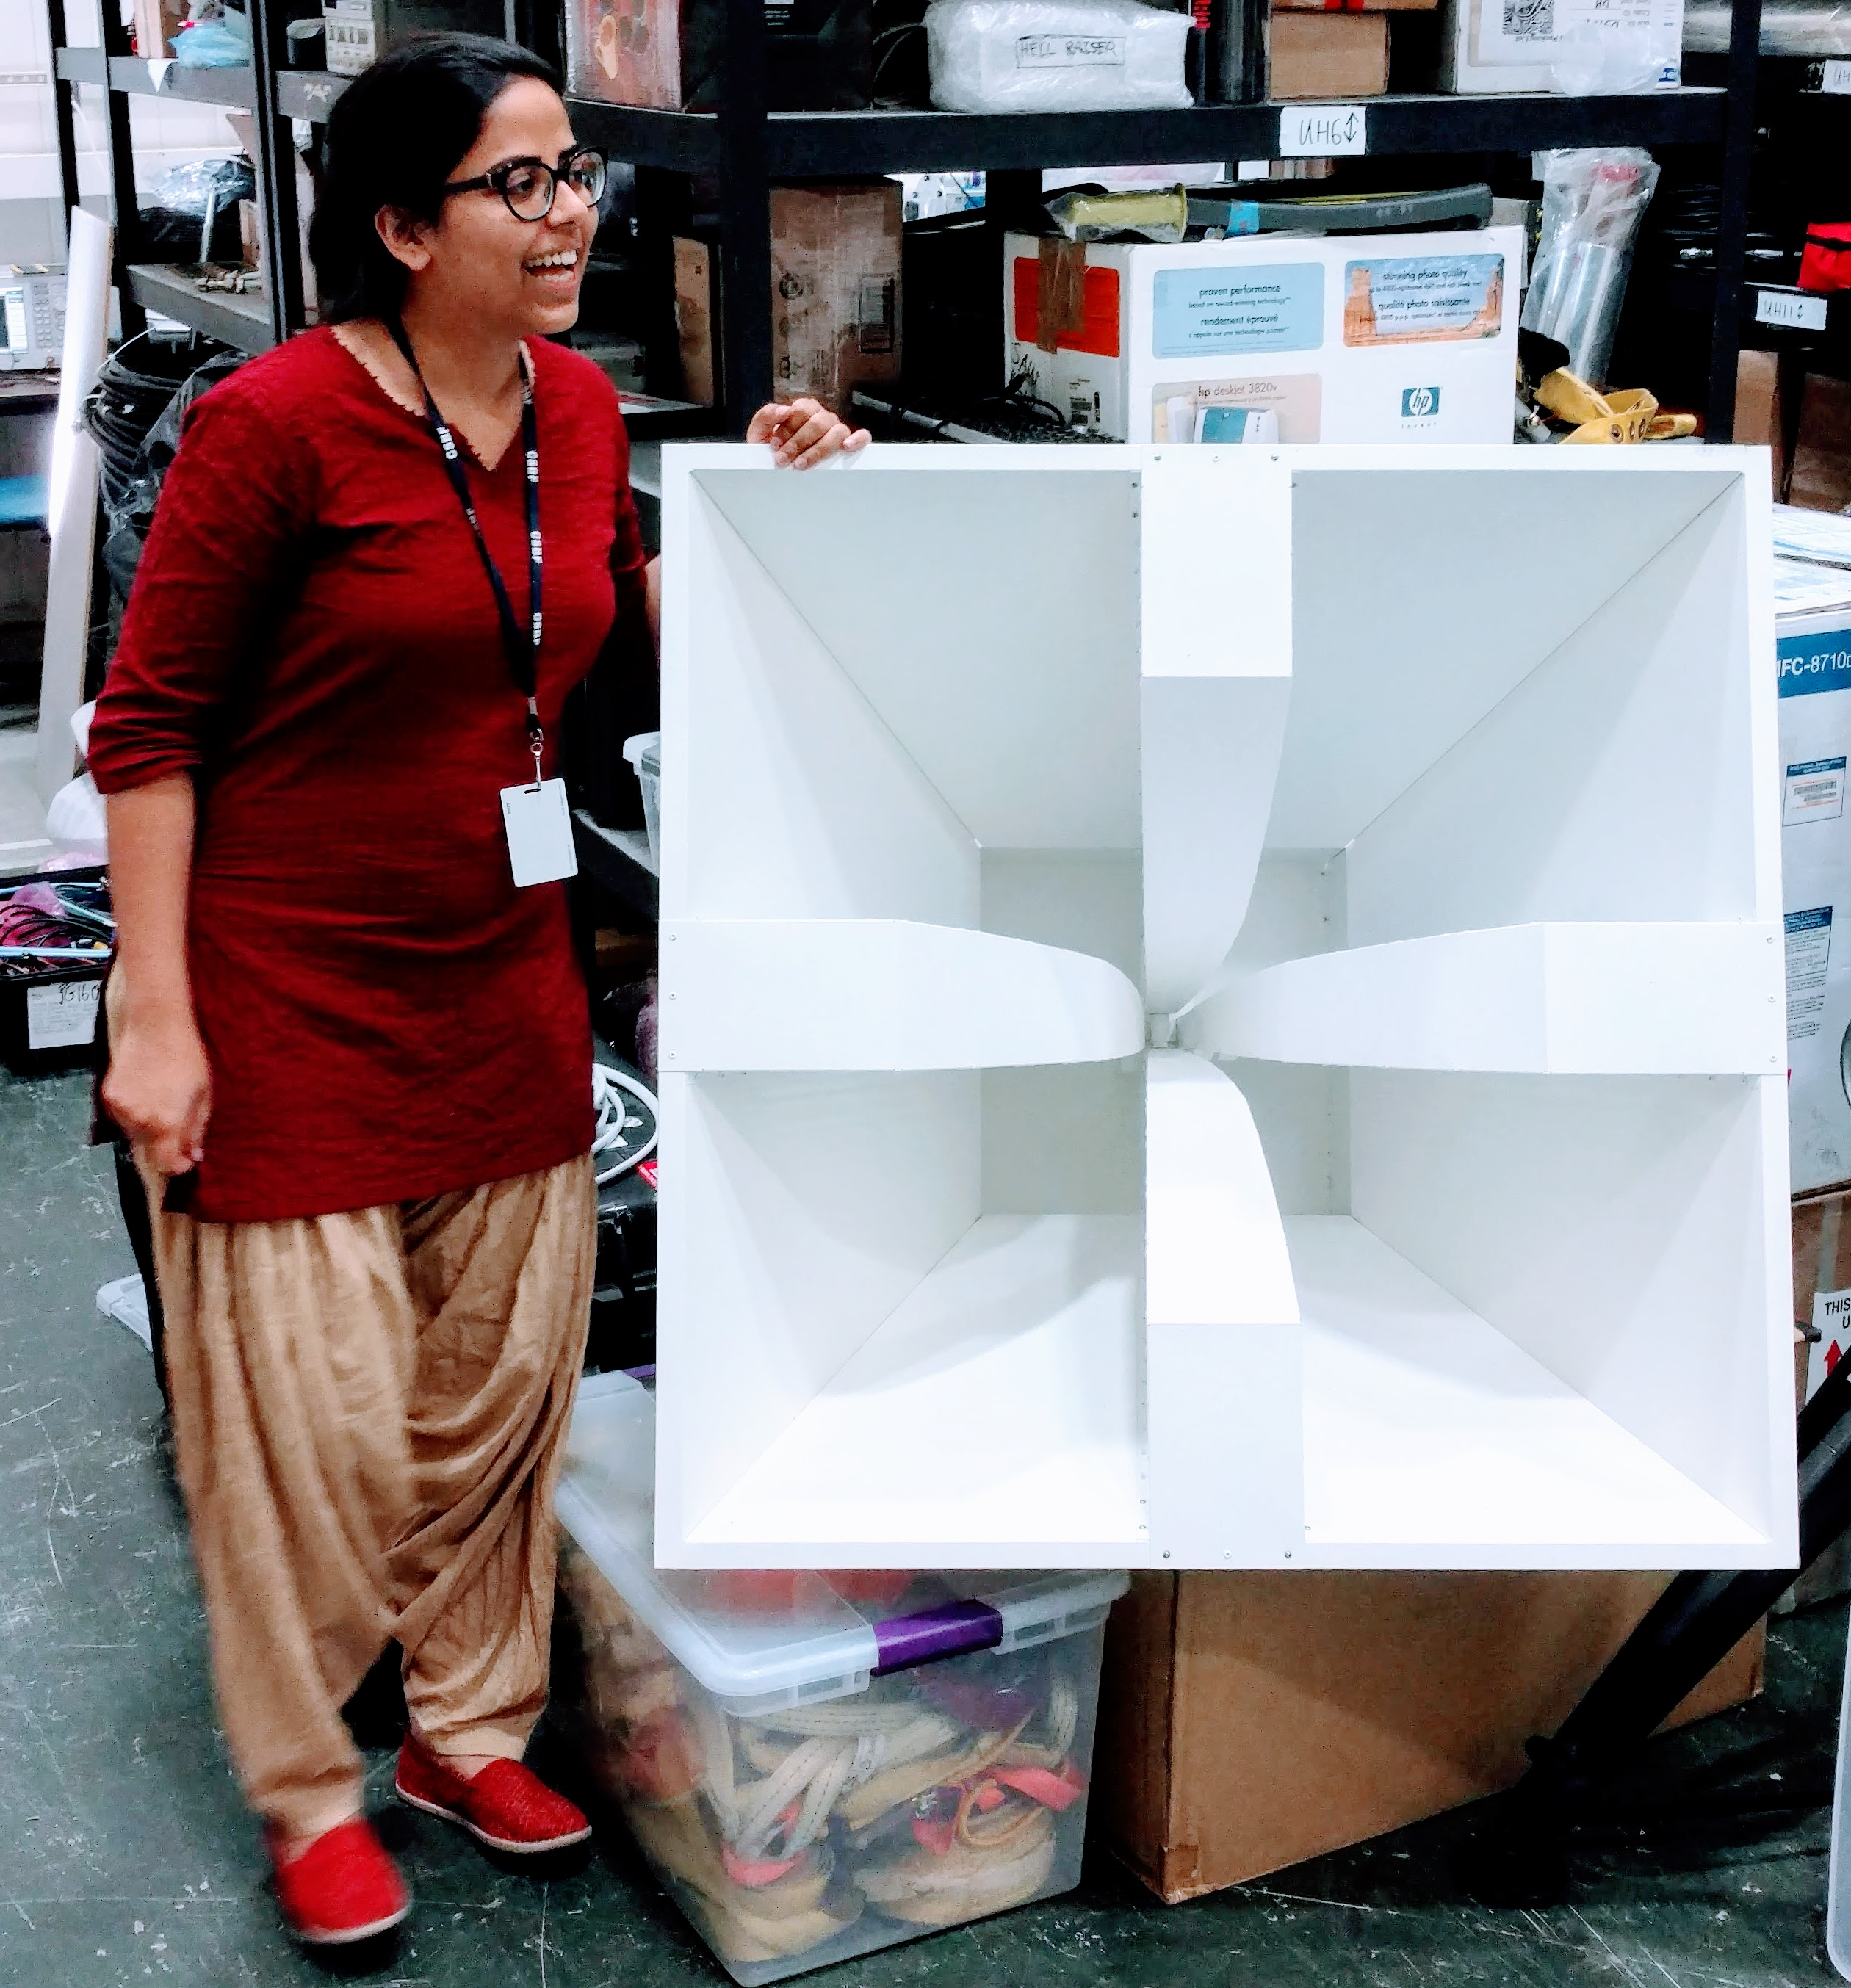
\includegraphics[width=1.0\textwidth]{figures/anita_antenna_me.jpg}
\caption{Here I am standing next to one of the ANITA horn antennas before the hang test of the ANITA-4 mission at Columbia Scientific Balloon Facility in Palestine, TX. Picture credit: Jacob Gordon.}
\label{antenna}
\end{figure}

\subsection{Radio antennas and Phi Sectors}

\gls{anita} looks for \gls{uhe} neutrinos with \gls{rf} antennas.
Figure~\ref{antenna} shows myself standing next to one of these antennas during the integration and testing of \gls{anita}-4 at the Columbia Scientific Balloon Facility in Palestine, TX in July of 2016. Custom-built by Seavey Engineering, they
are $0.8\,\mbox{m}$ long on a side, quad-ridged and horn-shaped.
The antennas are broadband and highly-directional. 
They have an on-axis gain of $\sim10\,\mbox{dB with respect to isotropic gain}$.
The $3\,\mbox{dB}$ point of these antennas is $\sim30^{\circ}$.


There are 48 antennas on the \gls{anita}-4 payload.
They are mounted on the ANITA gondola covering $360^{\circ}$ in azimuth. 
%Each antenna has two perpendicular feeds allowing detection of horizontally polarized and vertically polarized signals. 
%There have been 32, 40, 48, and 48 antennas on the \gls{anita}-1, 2, 3, and 4 flights, respectively.
The antennas are arranged in three aligned rings of 16 antennas, termed the top, middle, and bottom rings. 
The top ring consists of two staggered sub-rings each having eight antennas. 
%The antennas are mounted on the payload's gondola which is made of aluminum for its light-weight. 
The \gls{fwhm} beamwidth of the antennas is approximately $45^{\circ}$. 
The antennas in the top ring are evenly spaced by $45^{\circ}$ in azimuth. 
The two sub-rings in the top ring are offset by $22.5^{\circ}$ for uniform coverage.
The antennas in the middle ring are evenly spaced by $22.5^{\circ}$.
The antennas in the bottom ring are evenly spaced by $22.5^{\circ}$.
All the antennas are angled downward by $10^{\circ}$ to preferentially observe signals coming from the ice as opposed to from the sky. 
Each group of three antennas in a vertical column, taking one antenna from each ring, forms a phi sector, viewing a $22.5^{\circ}$ region in azimuth.

The antennas are dually-polarized with a feed each for \gls{hpol} and \gls{vpol} signal.
\gls{rf} signal through each channel goes through the 
\gls{ampa} unit before entering the Instrument Box. 
There is an \gls{ampa} unit connected directly to the \gls{hpol} and \gls{vpol} outputs of each antenna. 
The \gls{ampa} contains a $200 - 1200\,\mbox{MHz}$ bandpass filter, followed by an approximately $35\,\mathrm{dB}$ Low Noise Amplifier (LNA). The \gls{ampa} performs the first-stage amplification of the incoming \gls{rf} signal. I led a camp (John Russell christened it ``Campa") at the ANITA headquarters, University of Hawaii, in September of 2016, to finish assembling these \gls{ampa} units for the \gls{anita}-4 flight. I show one of the 100 that I worked on assembling in Figure~\ref{ampa}. These even involved a bit of careful soldering and using the heat gun!

\begin{figure}
\centering
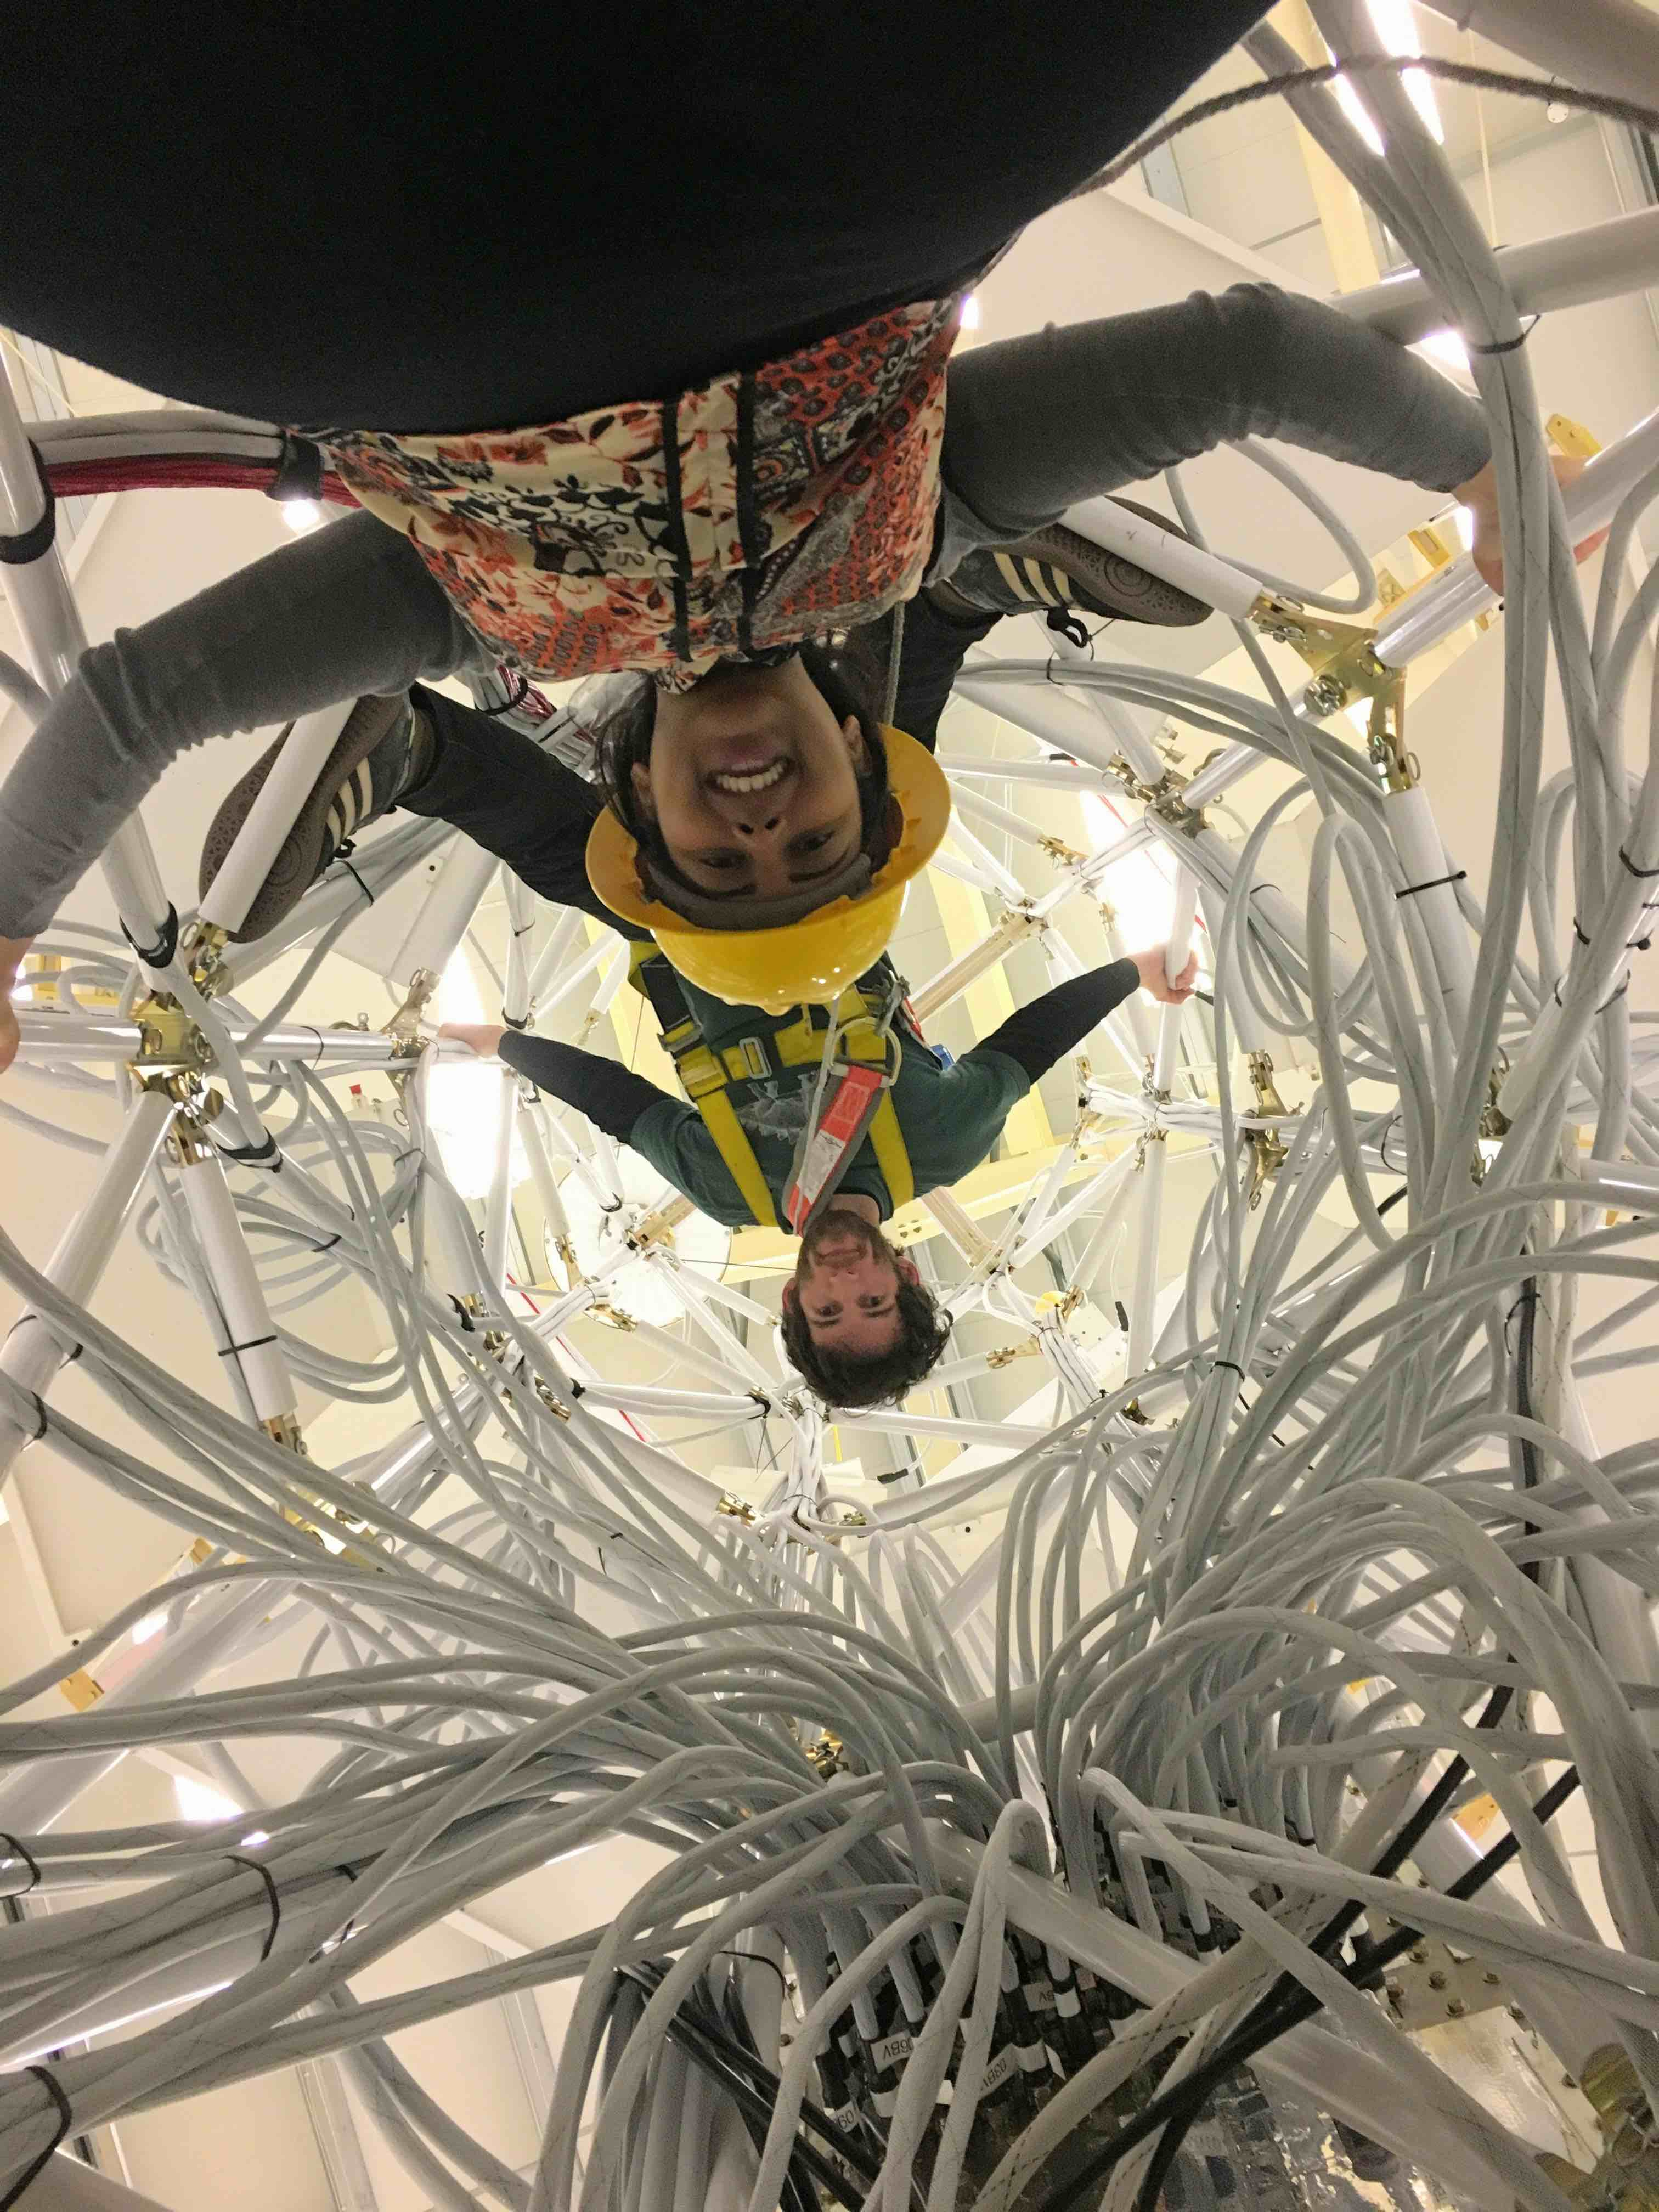
\includegraphics[width=0.52\textwidth]{figures/beams.jpg}
\caption{Andrew Ludwig and I working on integration and cabling of ANITA-4 at the NASA LDB facility near McMurdo Station, Antarctica. The aluminum beams that form the underlying structure of the payload can be seen here. Light aluminum beams help to abide by weight restrictions. Image credit: Nan Wang.}
\label{hanging}
\end{figure}

\begin{figure}
\centering
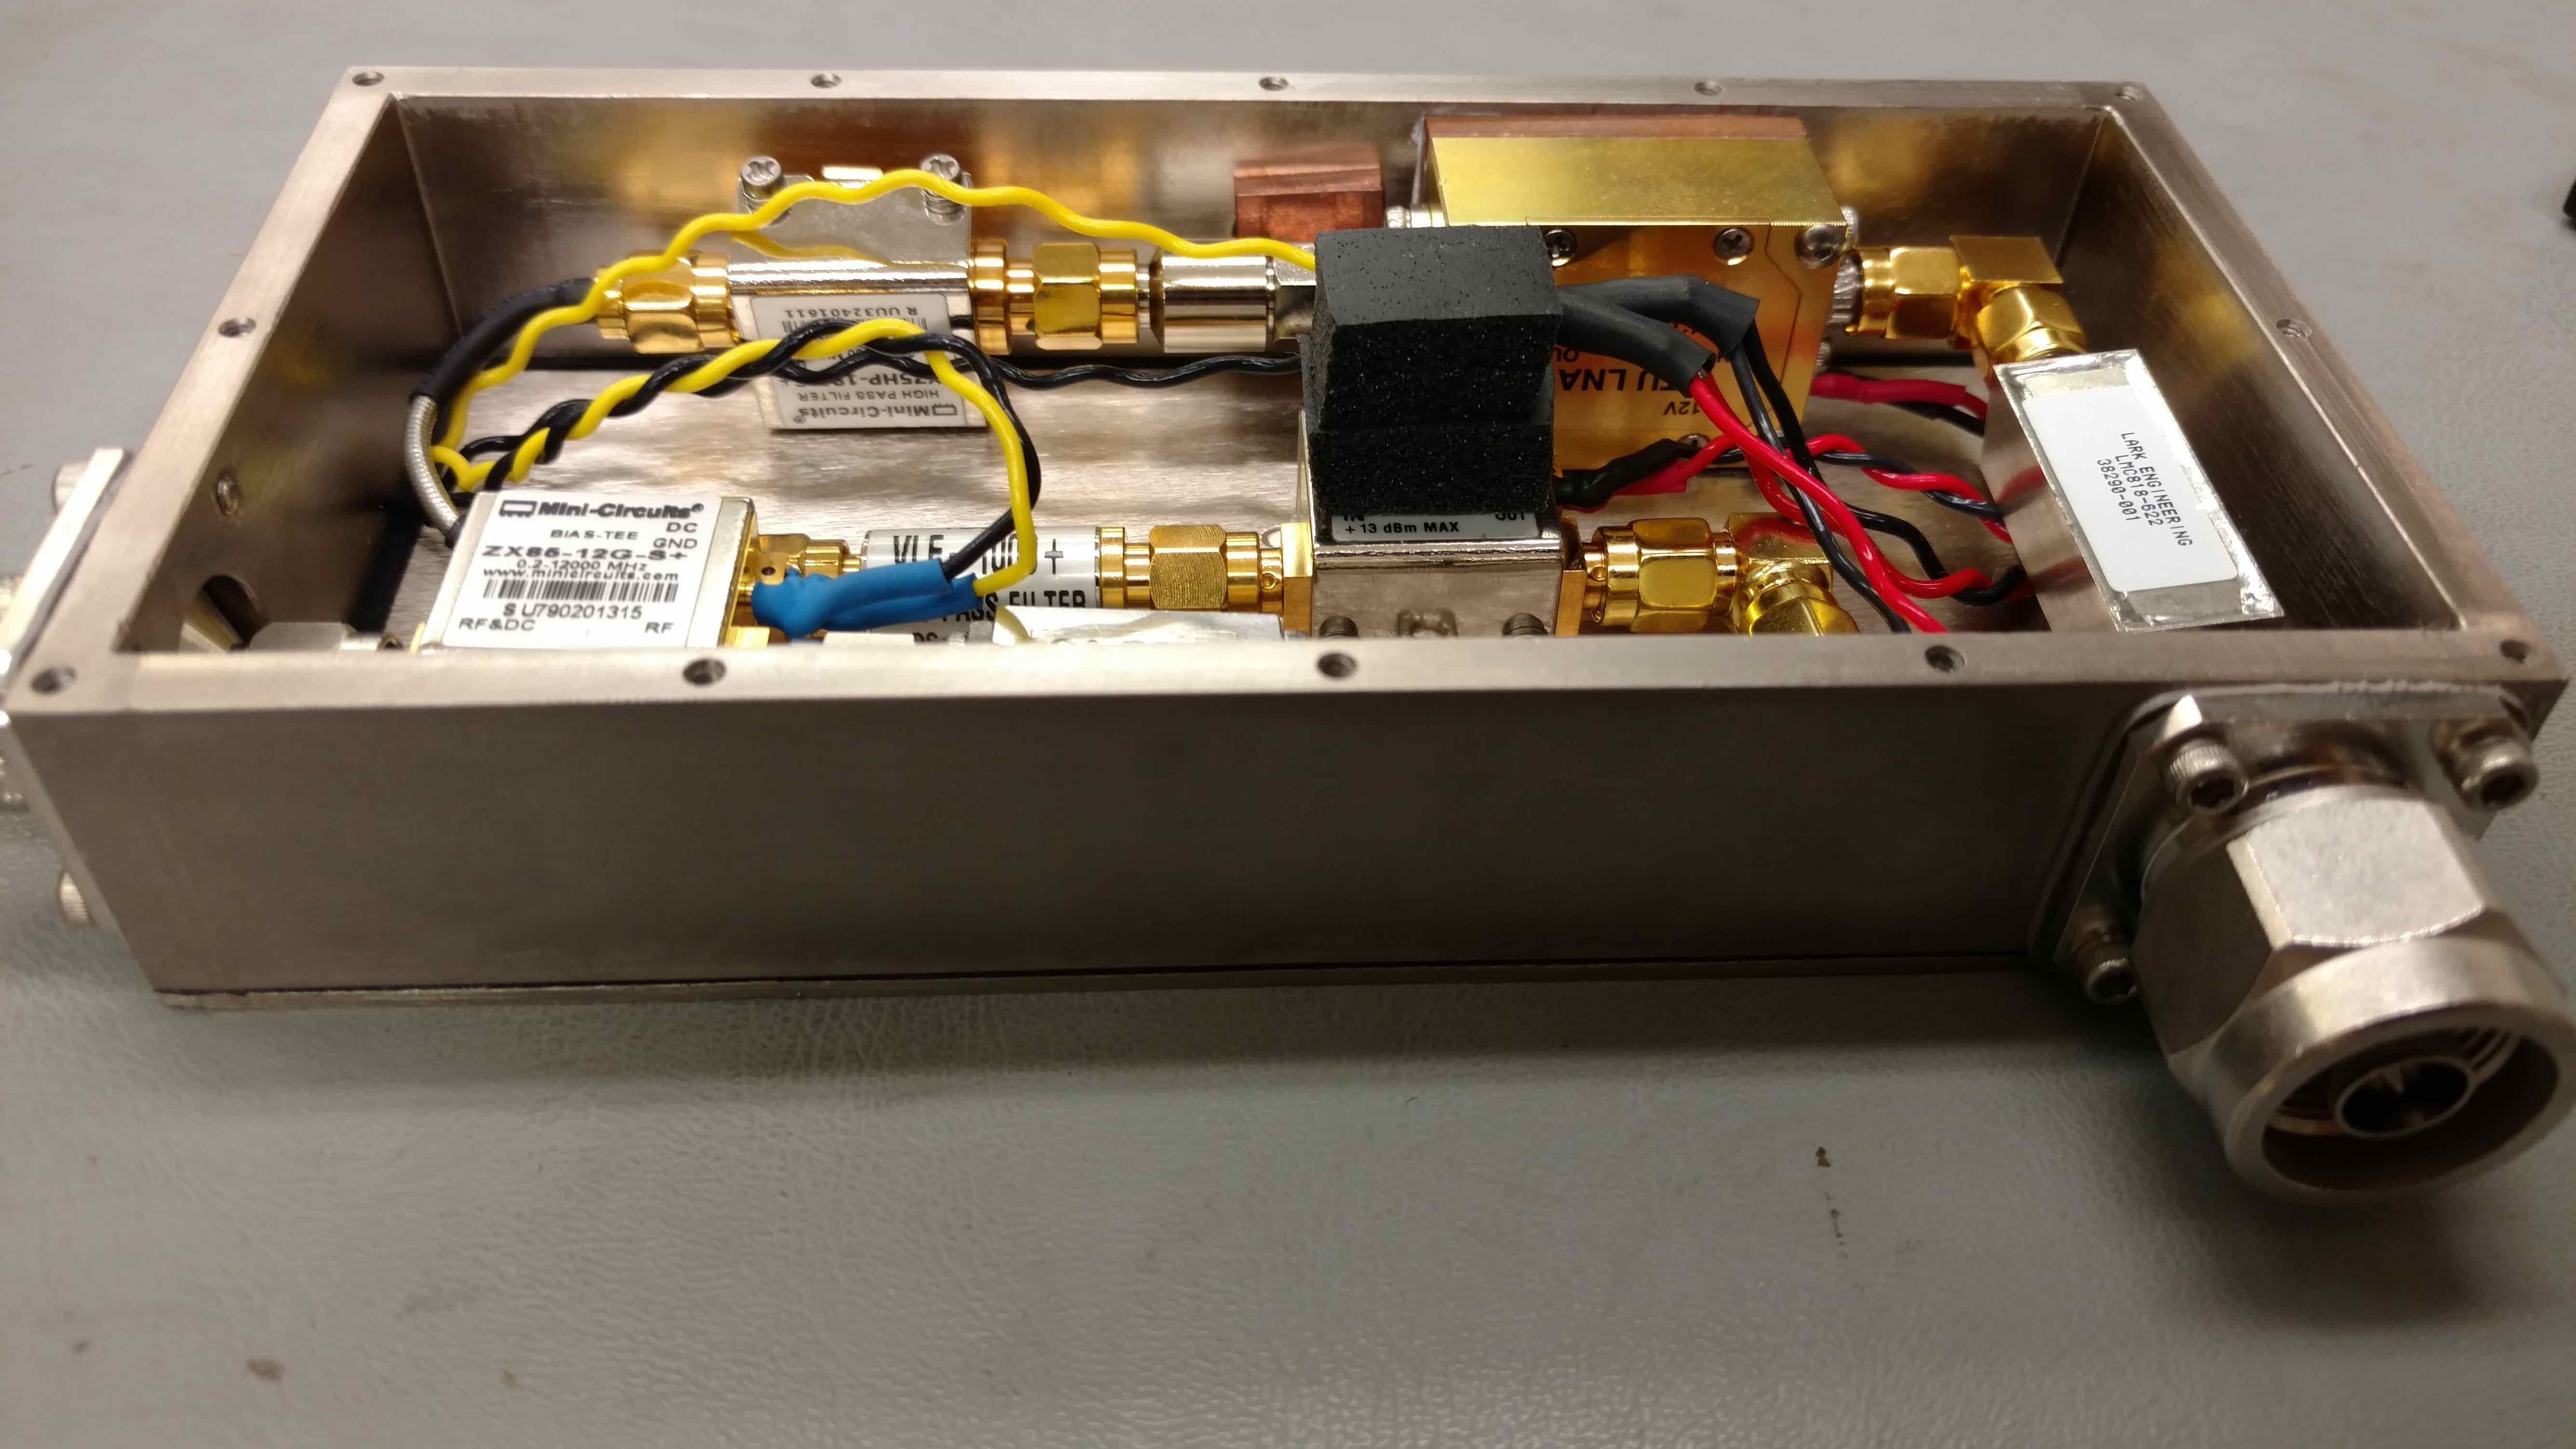
\includegraphics[width=1.0\textwidth]{figures/ampa.jpg}
\caption{Rare picture of the inside of an AMPA from ANITA-4.}
\label{ampa}
\end{figure}

\subsection{Instrument Box and Science Instrument Package}
\label{box_sip}

The Instrument Box of ANITA sits on the payload's deck. 
Most of the signal processing in \gls{anita} takes place inside the Instrument Box.  
Following the \gls{ampa} unit, the \gls{rf} signal travels through $12\,\mbox{m}$ of
LMR240 coaxial cable to the Instrument Box. 
Inside the Instrument Box, the signal first goes through second-stage amplification and notch filtering both performed by the \gls{tuff} boards in ANITA-4.
Then it passes through another set of bandpass filters before
being split into digitization and triggering paths. 
The triggering and digitization processes are detailed in~\cite{tuff}. 

The \gls{sip} also sits on the payload's deck. 
The SIP is powered and controlled by NASA.
It is used for flight control such as ballast release and flight termination. 
The SIP also provides a connection to the ANITA payload during flight through line-of-sight transmission, the Iridium satellite, and the Tracking and Data Satellite System (TDRSS). 
This allows us to monitor the payload continuously during the flight.
A small fraction of data (less than 1\%) is transferred from the payload through telemetry.
Commands to perform different functions, such as tuning a \gls{tuff} notch filter, 
%or altering a trigger threshold, 
can be sent to the payload in real time using the SIP connection. 

\subsection{Power}
\label{power}

There are unusual constraints on the total power budget of ANITA as it is a balloon payload. 
The ANITA-3 and ANITA-4 payloads operated on $\sim500\,\mathrm{W}$ and $\sim600\,\mathrm{W}$ respectively.
The payload is solar-powered by photovoltaic (PV) cells. 
One set of PV cells are on top of the gondola. 
These are managed by NASA and used to power the SIP. 
The other set is termed the ``drop-down PV array" and the PV cells in this set are arranged in eight 90-cell strings, laid out in an octagon around the bottom of
the payload. 
The drop-down PV array powers the Instrument Box. 
Before launch, they partially cover up the antennas in the bottom ring, as seen in Figure~\ref{anita}. 
After launch, the eight strings are remotely instructed to drop down by the SIP, which fires a servo to deploy them below the bottom ring of antennas. 

A charge controller distributes the output from the drop-down PV array to the payload as $24\,\mbox{V}$, using DC-DC converters 
to provide $12\,\mbox{V}$, $-12\,\mbox{V}$, $3.3\,\mbox{V}$ and $5\,\mbox{V}$ to various systems. 
The charge controller is also connected to a battery farm of $12\,\mbox{V}$ lead-acid batteries. 
Although there is daylight 24/7 in the Antarctic summer, the amount of power the PV array produces changes with the Sun's elevation during each 24 hour period. Thus, a battery farm is needed as backup. 
When the PV array is able to power the payload by itself, the charge controller charges the battery farm. 
This is in the Battery Box which is also placed on the deck. 

\subsection{GPS Systems and Heat dissipation} 
\label{gps_heat}

\gls{anita} data analysis relies on location and orientation information of the payload. 
\gls{anita} uses three GPS systems during flight: ADU5A, ADU5B and G12. 
These GPS antennas are located on top of the payload.
The ADU5 systems provide heading, pitch and roll information.
The G12 system updates absolute time on the flight computer through its Network Time Protocol (NTP) server. 
As backup to the GPS systems, there are four sun-sensor instruments, a magnetometer and accelerometer located on the deck. 

%\subsection{Heat dissipation}
At high altitudes of $35\,\mbox{km}$ and above, the primary method of heat loss is radiation. 
Thus, many parts of the payload are painted white to reflect sunlight and regulate temperature. 
Components producing large amounts of heat are connected to a teflon-coated, silver-tape-lined radiator plate on the Instrument Box.

\section{ANITA Signal Processing}

In this section we describe the signal processing chain for ANITA-4, and in particular
the steps that are relevant to understanding the role of the \gls{tuff} boards.
We will note when and where the ANITA-3 signal processing differed.
Note that much of the contents of this section is also covered in~\cite{tuff}. 
The \gls{rf} signal processing chain for ANITA-4 is illustrated in Figure~\ref{system}. 

\begin{figure}
\centering
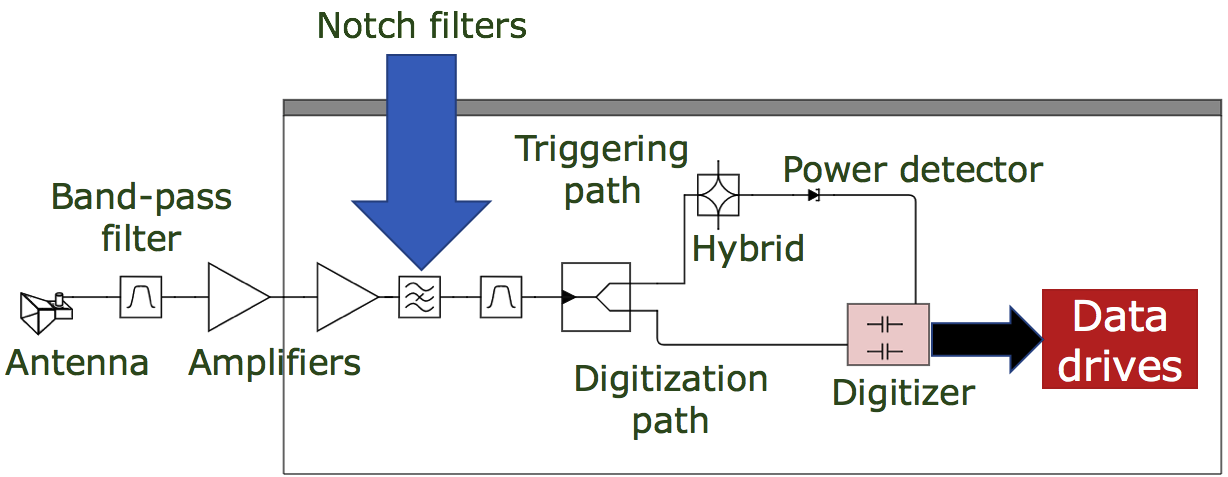
\includegraphics[width=1.0\textwidth]{figures/A4_simple_system.png}
\caption{Simplified form of the signal processing chain in ANITA-4. A more detailed diagram can be found in \cite{tuff}. The blue solid arrow shows where the TUFF notch filters are in the chain. More details on the TUFF boards and notch filters are presented later in this chapter.}
\label{system}
\end{figure}

\subsection{Triggering}
\label{trigger}

In the triggering path, the \gls{rf} signals from both the \gls{vpol} and \gls{hpol} channels of a single antenna 
are passed through a $90^{\circ}$ hybrid (hybrids were absent in ANITA-3). 
The outputs from the $90^{\circ}$ hybrid are the left- and right- circular polarized
(LCP and RCP) components of the combined \gls{vpol} and \gls{hpol} signals from an antenna. 
The hybrid outputs are input to the SURF (Sampling Unit for \gls{rf}) high-occupancy \gls{rf} Trigger (SHORT) unit before being passed to the SURF board. 
Each SHORT takes four channels as its input. 
In a SHORT
channel, the \gls{rf} signal passes through a tunnel diode and an amplifier. 
The output of the SHORT is
approximately proportional to the square of the voltages
of the input \gls{rf} signal integrated over approximately $5\,\mbox{ns}$.
It is a measure of the power of the incoming signal and is typically a negative voltage.
The SHORT output is routed to a SURF trigger input where 
it enters a discriminator that compares this negative voltage in Digital-to-Analog Converter (DAC) counts to the output
of a software-controlled DAC threshold on the SURF, henceforth referred to as the SURF DAC threshold. 
The SURF DAC threshold is expressed in arbitrary units of DAC counts corresponding to voltages. Lower thresholds 
correspond to higher voltages and therefore, higher power of the incoming signal. 
The SURF DAC threshold can be changed during flight. Thresholds for the \gls{anita}-3 and -4 flights are shown in Figure~\ref{thresholds_fig}. 
During the ANITA-3 flight, CW interference overwhelmed the digitization system, forcing us to impose
frequent and large changes in the SURF DAC thresholds. 
%A comparison of SURF DAC thresholds between ANITA-3 and ANITA-4 is presented in Figure~\ref{thresholds}.
Note that the lower overall threshold for ANITA-4 is primarily due to the modified triggering scheme, 
which requires more overall coincidences between channels. 
The increased stability of the ANITA-4 thresholds, due to the CW mitigation schemes presented later, is clearly apparent.

\begin{figure}
\centering
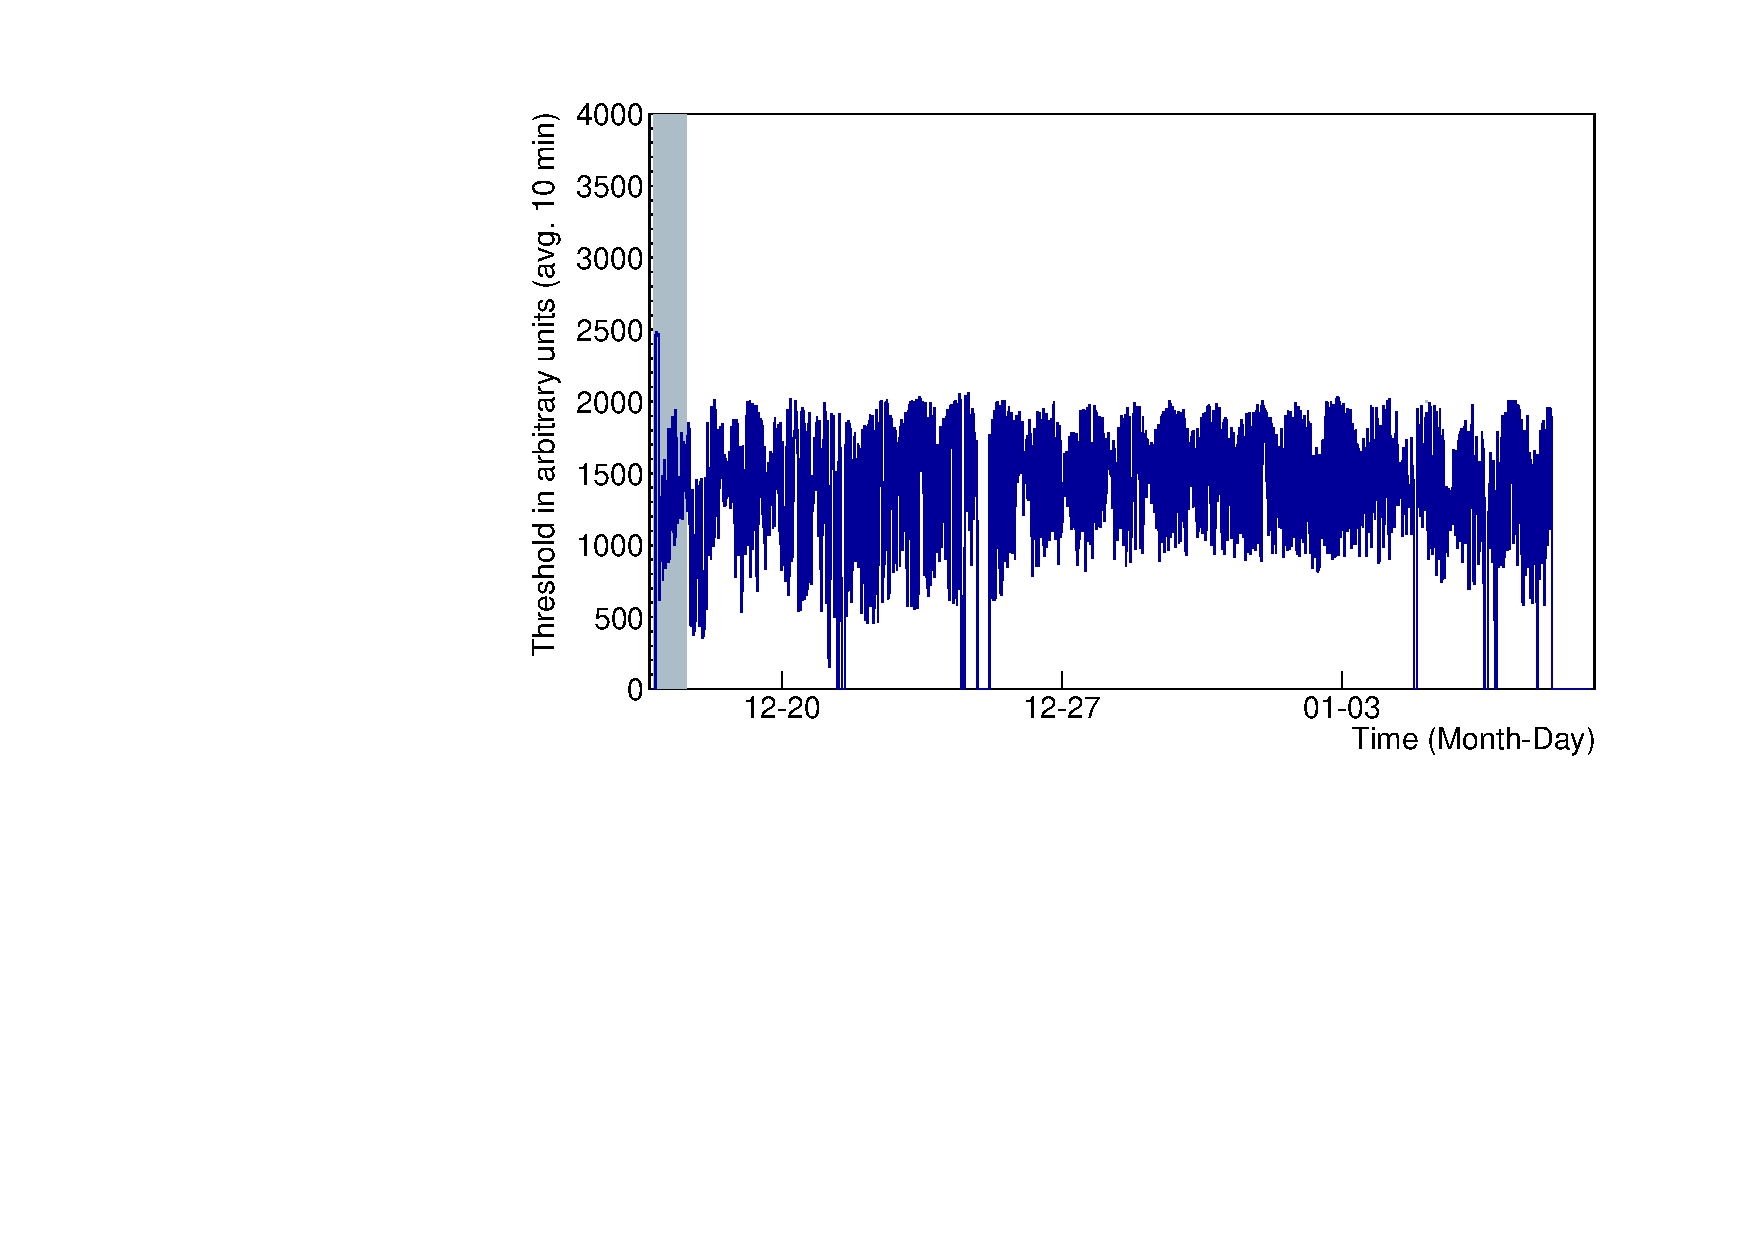
\includegraphics[width=1.0\textwidth]{figures/anita3_threshold_time20_2.pdf}
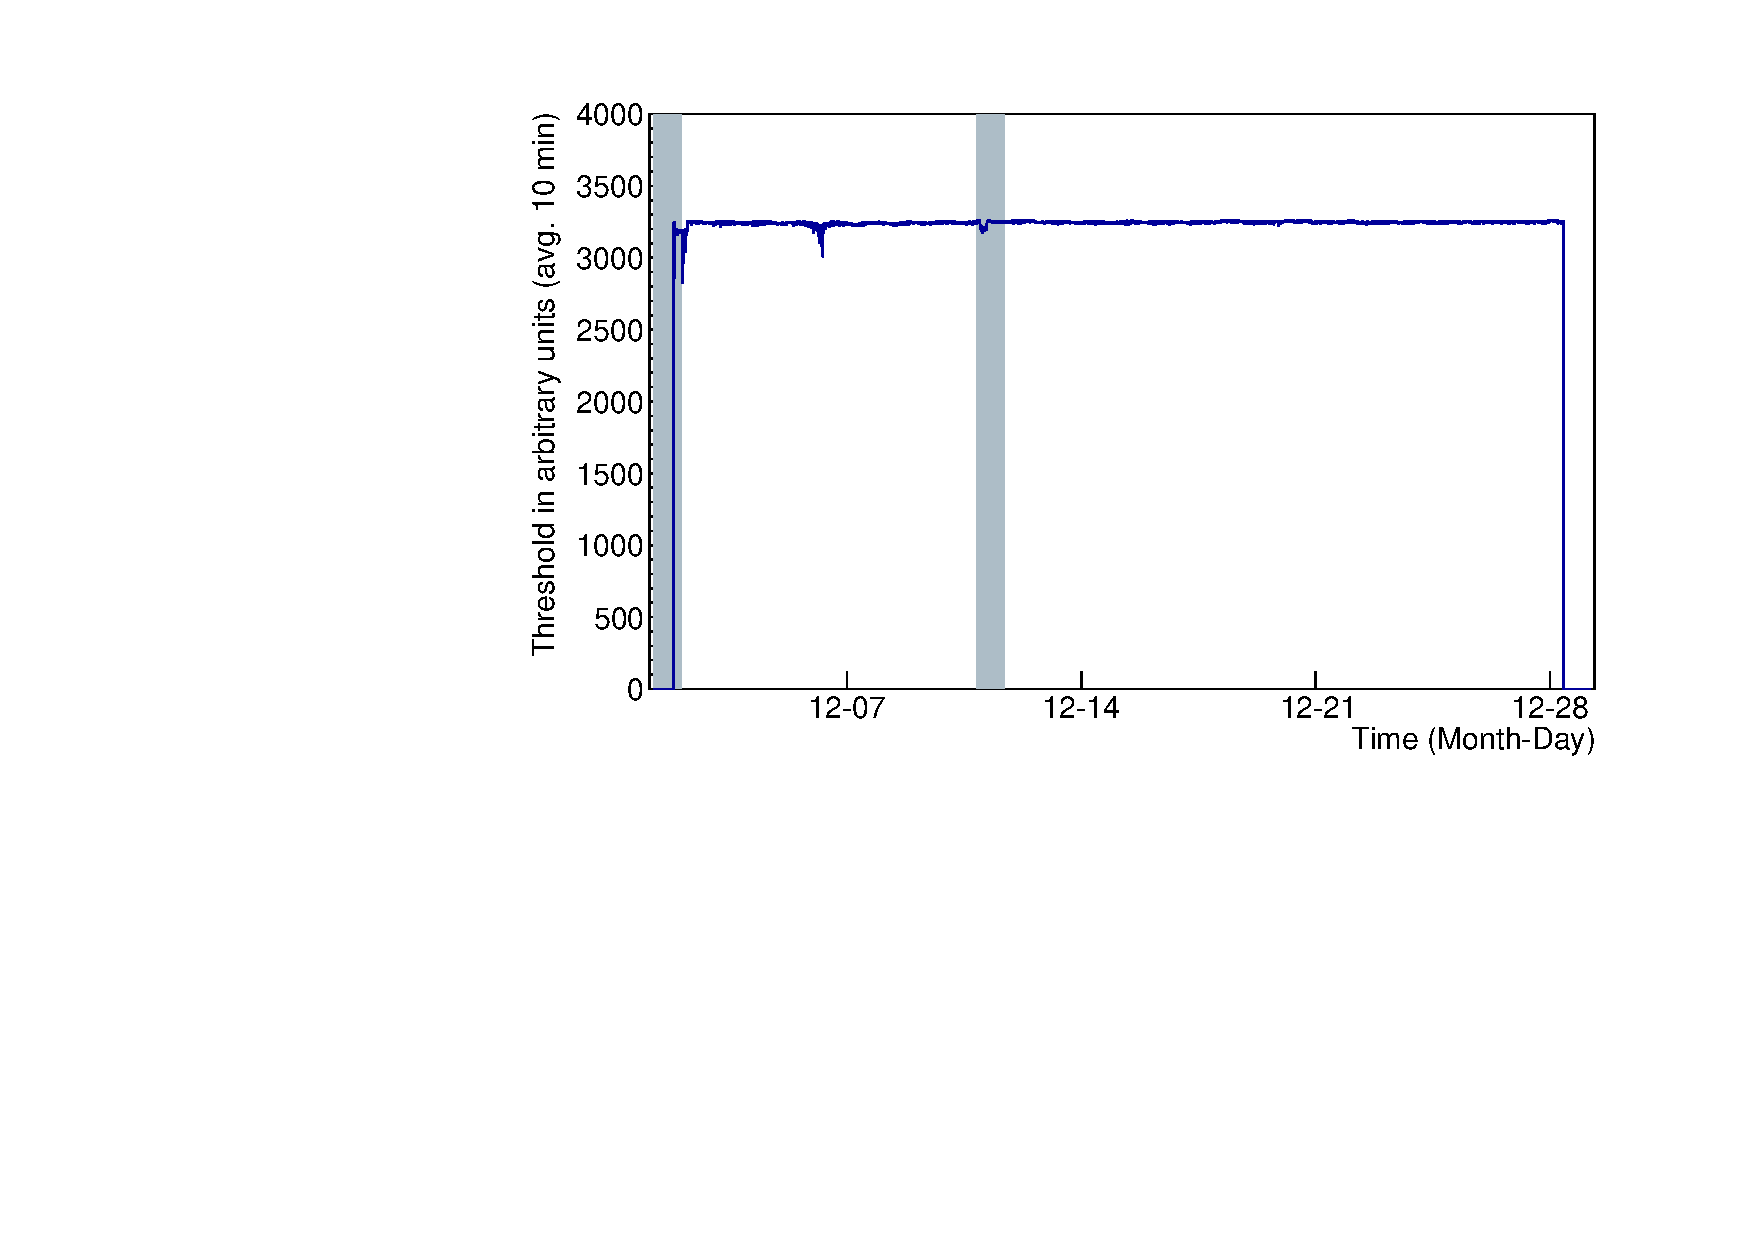
\includegraphics[width=1.0\textwidth]{figures/anita4_threshold_time_2.pdf}
\caption{Thresholds during the ANITA-3 (top) and ANITA-4 (bottom) flights.}
\label{thresholds_fig}
\end{figure}


\paragraph{Trigger logic:}
Due to power and bandwidth limitations, ANITA is not able to constantly record data. 
Digitization of data only occurs when the trigger conditions are satisfied.
The ANITA-4 trigger consists of three triggering levels: Level~1, Level~2 and Level~3. 
The trigger requirements at each of these three levels is described below.

\paragraph{Level~1 trigger:}

The Sampling Unit for \gls{rf} (SURF) board issues the Level~1 trigger.
To form a Level~1 trigger, the SHORT outputs of the LCP and RCP channels from the same antenna 
are required to exceed the SURF DAC threshold within $4\,\mbox{ns}$. This LCP/RCP coincidence requirement 
was added to the ANITA-4 trigger to mitigate anthropogenic and thermal backgrounds.
The signals of
interest are known to be linearly polarized, whereas satellite emission is often circularly polarized
and thermal noise is unpolarized. In the presence of a continuous source of CW signal such as satellites,
the LCP/RCP coincidence may still allow a combination of circularly polarized satellite noise and the circularly polarized component of
thermal noise to satisfy the Level~1 trigger requirement. Therefore, the LCP/RCP coincidence aids in
reducing triggers induced by satellites but does not completely mitigate their effect.

\paragraph{Level~2 trigger:} 

The SURF board issues the Level~2 trigger. 
A Level~1 trigger opens up a time window.
If there are two Level~1 triggers in the same phi sector within the allowable time window, then a Level~2 trigger is issued. 
The allowable time window depends on which antenna had the first Level~1 trigger. 
Time windows of
$16\,\mbox{ns}$, $12\,\mbox{ns}$ and $4\,\mbox{ns}$ in duration are
opened up when a Level~1 trigger is issued in the bottom, middle and top ring respectively.
These time windows were chosen to preferentially select signals coming up from the ice. 
The Level~2 trigger decisions are passed from the SURF boards to a dedicated triggering board called the Triggering Unit for \gls{rf} (TURF).
The Level~2 trigger timing in ANITA-4 differed from that used in ANITA-3 as changes were made to further restrict
the allowed timing of the antenna coincidences to 
better match timing expected from an incoming plane wave.

\paragraph{Level~3 trigger:}

The TURF board issues the Level~3 trigger.
A field programmable gate array (FPGA) on the TURF board monitors Level~2 triggers.
A Level~3 trigger is issued by the TURF board when there are Level~2 triggers in two adjacent phi sectors within $10\,\mbox{ns}$. 
When there is a Level~3 trigger, the TURF board instructs 
the SURF board to begin digitization.

\subsection{Digitization}

The digitization of the signal is performed by the SURF board. 
There are twelve SURF boards, each containing four custom-built Application Specific Integrated
Circuits called \gls{lab}. 

\paragraph{\gls{lab} chip and digitization deadtime:}
ANITA-4 uses the third generation
of \gls{lab} chips that are described by Varner \textit{et al}. \cite{labrador}. 
Each \gls{lab} chip has a 260-element switched capacitor array (SCA) for each of its 9 input channels, with one channel used for timing synchronization.
The \gls{rf} signal entering a SURF gets split and fed into four parallel \gls{lab} chips (forming four ``buffers" for digitization). 
The SCAs sample waveform data at the rate of $2.6\,\mbox{GSa/s}$. 
At any moment, the charge stored in an SCA is a $100\,\mbox{ns}$ record of the signal voltage. 
This $100\,\mbox{ns}$ snapshot of the incoming plane wave is known as an ``event."
When a Level~3 trigger occurs, a single \gls{lab} chip stops sampling and is ``held.'' It then digitizes
the stored data, which is then read out by the flight computer, taking approximately $5-10\,\mbox{ms}$.
If all four \gls{lab} chips are held, the trigger is ``dead'' and the accumulated time when the trigger is dead is recorded as
digitization deadtime by the TURF board. 

\paragraph{Masking:}

During ANITA-3, digitization deadtime due to high levels of anthropogenic noise was reduced
by excluding
certain phi sectors from participating in the Level~3 trigger. 
This is called phi-masking. 
Alternatively, specific channels (each antenna has two channels) were excluded from participating in the Level~1 trigger. 
This is called channel-masking.
Together these are referred to as masking.
Because of CW interference by military communications
satellites, over half of the payload had to be masked
during most of the ANITA-3 flight. 
This strongly motivated the creation of the \gls{tuff}
boards with tunable, switchable notch filters. 
%A comparison of masking between \gls{anita}-3 and \gls{anita}-4 is presented in Figure~\ref{phimasking}. 

\paragraph{Data storage:}
All \gls{anita} data is stored on-board with less than 1\% of it transmitted to the ground during flight by telemetry. This is why payload recovery is critical. 
The primary storage devices are two
HGST UltraStar He6 disks, each with $6\,\mathrm{TB}$ capacity. 
These two Helium
drives contain identical copies of the data for redundancy in case of a drive failure.
Additionally, there are six $1\,\mathrm{TB}$ Solid State Drives for secondary data storage. 

\section{Tunable Universal Filter Frontend}
\label{tuff}

For ANITA-4, we built and deployed 16 \gls{tuff} boards (not counting spares) with 
six channels each for the 96 total full-band \gls{rf} channels of ANITA. 
Figure~\ref{system} shows, for a single \gls{rf} channel in ANITA-4, where 
the \gls{tuff} boards are in the signal processing chain. Details on these boards, their function and performance, as well as a portion of the contents of this section, are presented in~\cite{tuff}. 
%However, most of the images that I include in this thesis are not already shown in the publication.

\subsection{The problem: modulated continuous wave interference} 

The principal challenge of the \gls{anita} experiment is to distinguish neutrino signals from \gls{rf} noise. 
The two main sources of noise are thermal radiation by the Antarctic ice and anthropogenic noise, much of which is modulated \gls{cw} interference. 

While Antarctica itself is relatively free of \gls{cw} transmissions, except for bases of human activity, transmissions from geosynchronous satellites are continuously in view.
The average \gls{fwhm} beamwidth of the \gls{anita} antennas is approximately $45^{\circ}$.
Although the \gls{anita} antennas are canted downward by $10^{\circ}$, the beam of the antennas extends to horizontal from the perspective of the payload and
above.  
The Antarctic science bases, the most prominent being McMurdo and South Pole Station, are more radio-loud than the rest of the continent, producing \gls{cw} interference, for example, in the $430-460\,\mbox{MHz}$ band. 

\begin{figure}
\centering
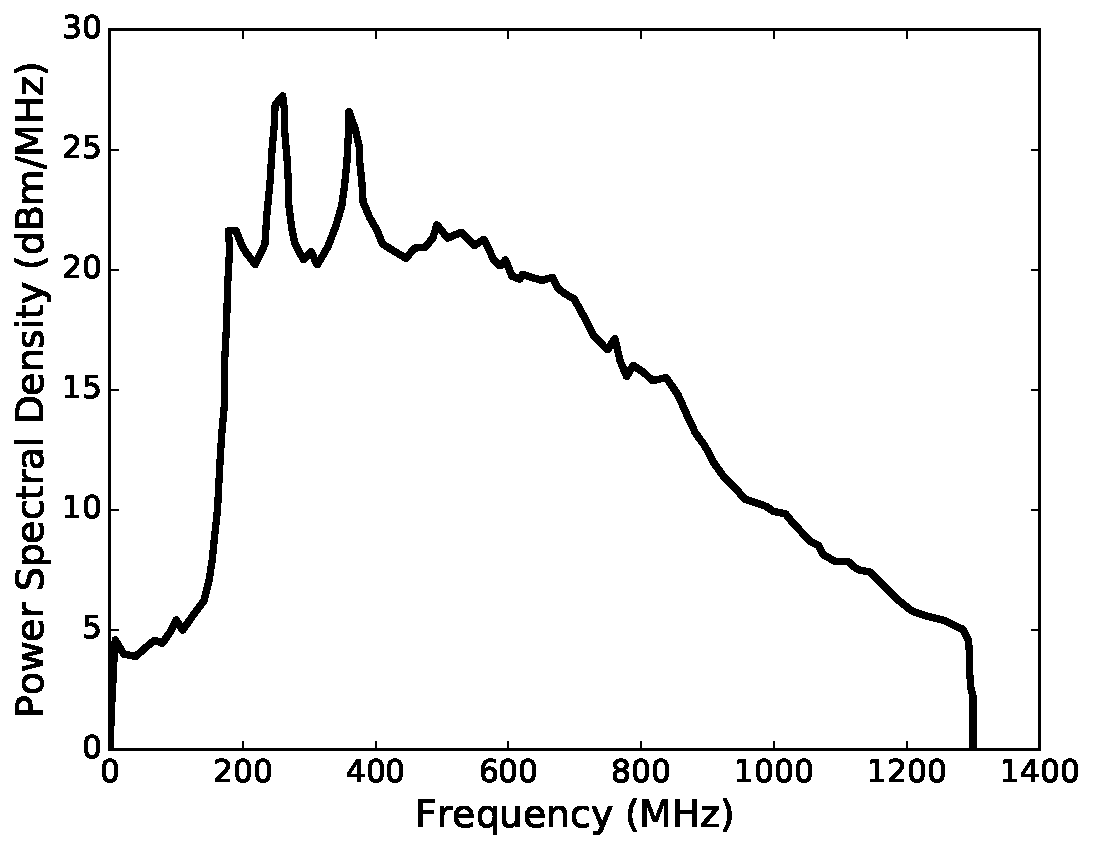
\includegraphics[width=1.0\textwidth]{figures/anita3spectra_wais_replot.pdf}
\caption{This averaged (over 2 mins) power spectrum shows the two CW peaks caused by military satellites that greatly reduced the instrument livetime (instrument livetime was only 31.6\%) of the ANITA-3 flight.}
\label{cw_peaks}
\end{figure}

\gls{cw} interference due to military satellites has affected all \gls{anita} flights.
\gls{anita}-1 (Dec. 2006 - Jan. 2007) and \gls{anita}-2 (Dec. 2008 - Jan. 2009) observed \gls{cw} interference primarily in the $240-270\,\mbox{MHz}$ band, peaking
at $260\,\mbox{MHz}$. This frequency range is predominantly used by the aging Fleet Satellite (FLTSAT) Communications System 
and the Ultra High Frequency Follow-On (UFO) System, both serving the 
United States Department of Defense since year 1978 and 1993 respectively.
In addition to \gls{cw} interference at $260\,\mbox{MHz}$, ANITA-III (Dec. 2014 - Jan. 2015) observed \gls{cw} interference at $375\,\mbox{MHz}$
which is thought to be due to
the newer Mobile User Objective System (MUOS) satellites that were launched during the period from Feb. 2012 - June 2016 \cite{milsat}.
The \gls{cw} signals generate events with excess power in left circular polarization (shown for the first time in Stafford's thesis~\cite{samStaffordThesis}) above the horizon, in approximately stationary positions.

The \gls{anita}-3 experiment was most affected by \gls{cw} interference due to military satellites. The first and second peaks in the power spectrum shown in Figure~\ref{cw_peaks} were present during all and about half, respectively, of the \gls{anita}-3 flight.
Due to the design
of the \gls{anita}-1 and \gls{anita}-2 trigger, which required coincidences among different frequency bands, the \gls{cw} interference did not overwhelm
the acquisition system. 
However, \gls{anita}-3 was redesigned for improved sensitivity and based its trigger decisions on full-bandwidth ($200 - 1200\,\mbox{MHz}$) signals. 
The modulation present in the \gls{cw} interference produced trigger rates far in excess of the digitization system's readout capabilities ($\sim50\,\mbox{Hz}$) for thresholds comparable to those used in previous flights. 
Thus, the \gls{anita}-3 experiment was susceptible to digitization deadtime throughout the flight. 

The lesson learned from the \gls{anita}-3 flight was
that a new method of mitigation of \gls{cw} signal was critical for the \gls{anita}-4 flight. 
Before \gls{anita}-4, the available methods to reduce digitization deadtime were masking
and decreasing thresholds when in the presence of higher levels of noise. 
A decrease in thresholds corresponds to higher power of the incoming signal. 
Masking and decreasing thresholds
come at the cost of instrument livetime~\cite{tuff} and sensitivity to neutrinos, respectively. 
%Both of these methods come at a high price.
For about 90\% of the time during the \gls{anita}-3 flight,
masking was used 
%during noisy periods 
to veto triggers from
over 
half of the payload field-of-view to keep the
trigger rate at or below $50\,\mbox{Hz}$. 
This significantly lowered the total instrument livetime. 
%Decreasing thresholds led to reduction of sensitivity to neutrinos during noisy periods. 
For \gls{anita}-4, the \gls{tuff} boards were built with
tunable notch filters to restore triggering efficiencies 
in the presence of CW interference. 
Additionally, the $90^{\circ}$ hybrids, previously deployed in \gls{anita}-1 as described in our design paper \cite{instrPaper}, were added to the \gls{anita}-4 trigger system by requiring a coincidence between left- and right- circularly polarized signals.
 
\begin{figure}
\centering
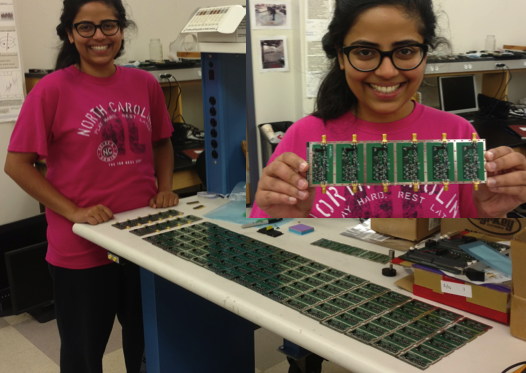
\includegraphics[width=1.0\textwidth]{figures/tuff_construction.png}
\caption{During the construction of the TUFF boards at OSU (May - July of 2016). The picture of myself holding one of the boards gives an idea for their size and shape. Clearly, building these boards made me very happy.}
\label{tuff_construction}
\end{figure}

\subsection{Design and construction}

In April of 2016, NASA gave the \gls{anita} collaboration the go ahead to attempt a launch of the \gls{anita}-4 mission at the end of that same year. From May - July of 2016, I worked on constructing and testing the \gls{tuff} boards. Constructing them involved soldering several thousand parts on to the boards. This was done by a small team at OSU, including myself, Jacob Gordon and Michael Kovacevich. Patrick Allison designed the boards and supervised our work. Testing of the boards was done in different stages and involved frequent measurement of the \gls{tuff} response using the network analyzer, making measurements of the board's current, capacitance, etc. with the multimeter, and performing experiments using the thermal and vacuum chambers. Figure~\ref{tuff_construction} shows myself holding a \gls{tuff} board and standing next to a freshly soldered batch of \gls{tuff} boards.

\begin{figure}
\centering
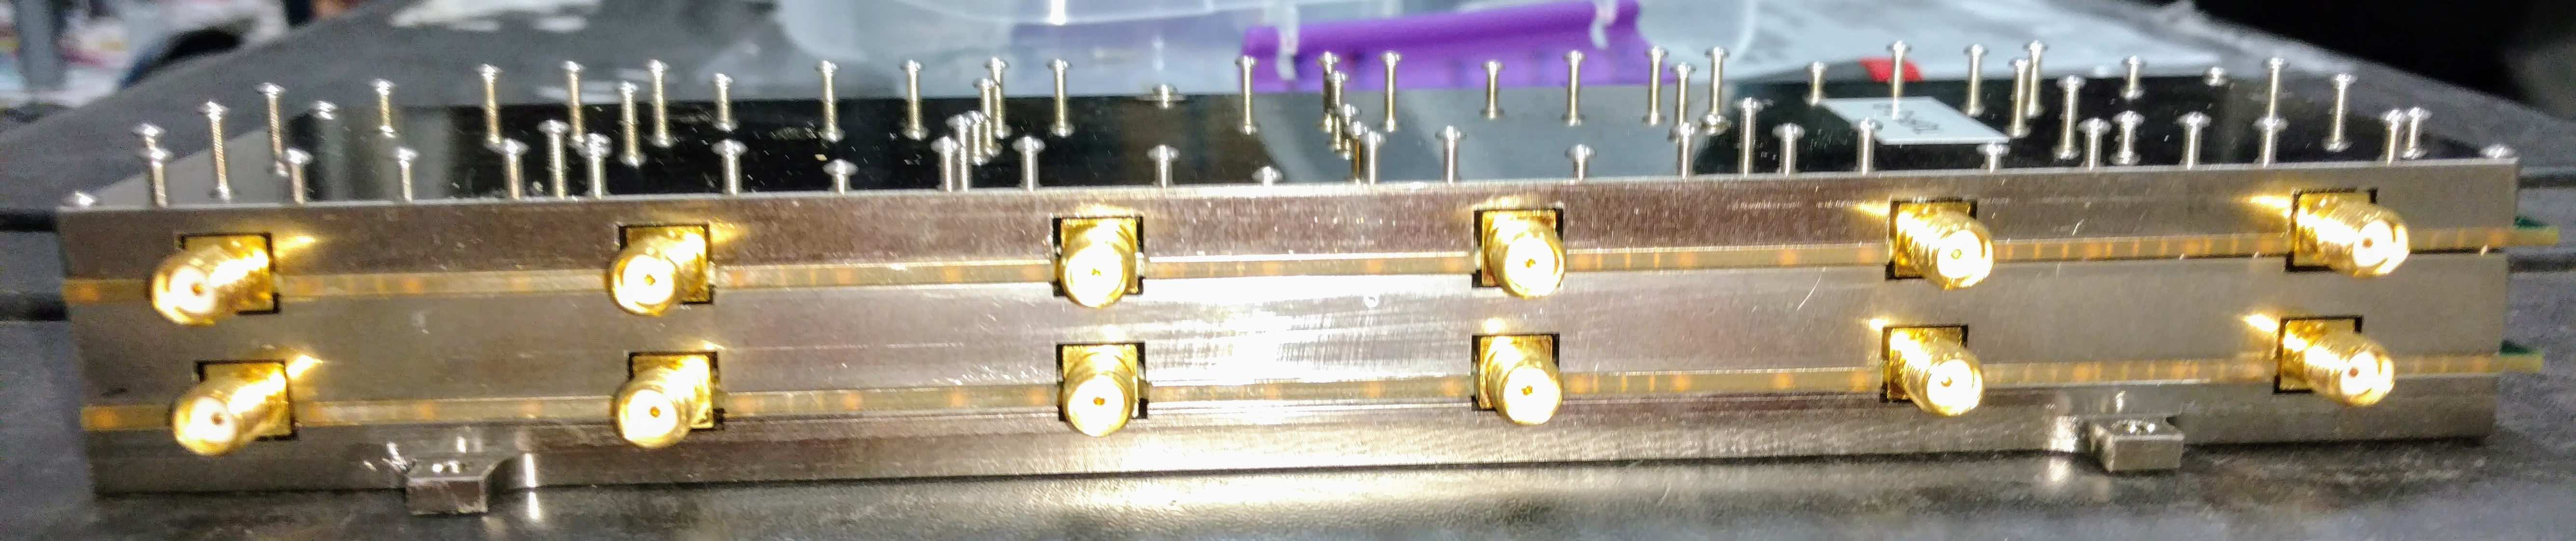
\includegraphics[width=1.0\textwidth]{figures/tuff_case_screws.jpg}
\caption{Pairs of TUFF boards were enclosed within aluminum cases with RF padding on the inside. The enclosures were held shut with the help of the screws shown here. Even a slight problem with the case design could make it very difficult to put the screws in or take them out. In fact, these screws became the bane of our existence during integration and testing of ANITA-4, and demonstrated how important it was to get the design of the cases right. Thanks to Christian Miki for designing the case.}
\label{case_screws}
\end{figure}

The design of the \gls{tuff} board was affected by the low power budget of \gls{anita} as well as the weight and size restrictions of a balloon mission, as described in Section~\ref{payload}. 
The \gls{tuff} boards needed to be low-power, compact and light. %Figure~\ref{tuff_channel} shows a single \gls{tuff} channel next to a quarter USD coin for size comparison. 
A single channel is about twice the size of a quarter dollar coin. 
Each printed circuit board has four layers of copper with an FR-4 dielectric material. 
%This is a composite made of woven fiberglass cloth with an epoxy resin binder that is flame resistant.
The \gls{tuff} boards operate on $3.3\,\mathrm{V}$ and $4.7\,\mathrm{V}$ power sources 
provided by
a MIC5504 from Microchip Technologies Inc. and a ADM7171 from Analog Devices Inc. Both
voltage regulators draw from a $5\,\mathrm{V}$ source 
supplied by the DC/DC unit in the ANITA
Instrument Box. 
A single \gls{tuff} channel consumes only $330\,\mathrm{mW}$ of power. 
The total power consumed by the ANITA payload is approximately $800\,\mathrm{W}$. 

Two \gls{tuff} boards were assembled into a final 
12-channel aluminum housing as shown in Figure~\ref{case_screws}. This provides heat-sinking, structural support, and \gls{rf} isolation. 
Two of these 12-channel modules were placed inside an 
\gls{irfcm} inside the Instrument Box of ANITA. Figure~\ref{irfcm} shows the inside of an IRFCM. Each \gls{tuff} channel has four main components which are described in the following subsections. 

\begin{figure}
\centering
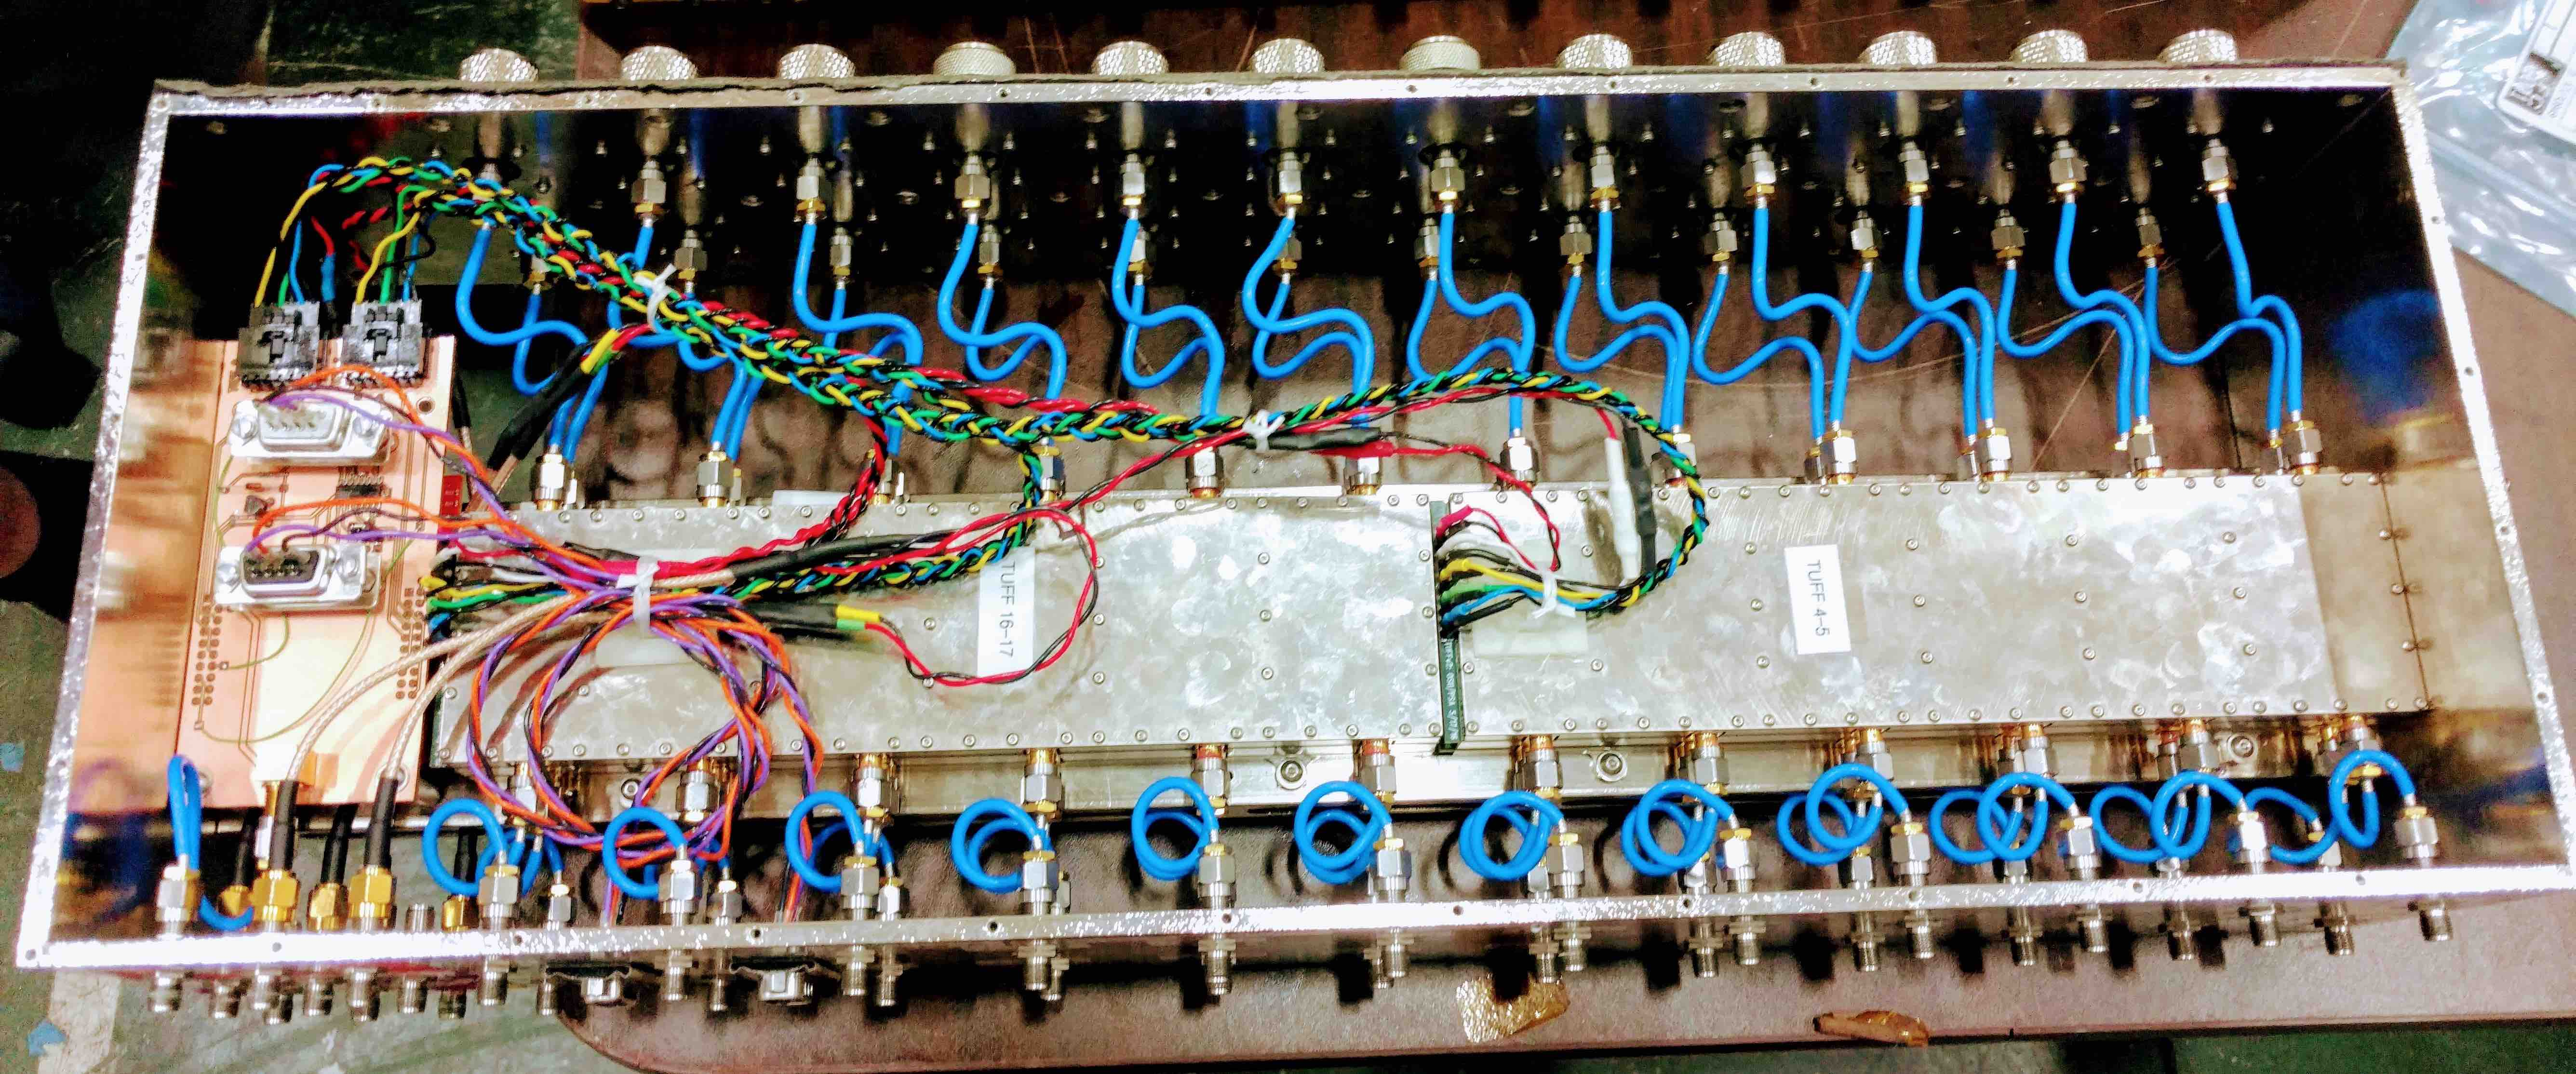
\includegraphics[width=1.0\textwidth]{figures/irfcm_thesis.jpg}
\caption{Rare picture of the inside of an Internal Radio Frequency Conditioning Module (IRFCM) holding two TUFF modules and a TUFF master. There are four total IRFCMs.}
\label{irfcm}
\end{figure}

\subsection{Amplifiers and bias tee} 

There are two amplifiers connected in series that together 
produce second-stage \gls{rf} power amplification of approximately $45\,\mathrm{dB}$. 
%The gain of a \gls{tuff} channel, as measured in the lab, is shown in Figure~\ref{s21}. 
AMP~1 is a BGA2851 by NXP Semiconductors and AMP~2 is an ADL5545 by Analog Devices. 
There is an attenuator producing $1\,\mathrm{dB}$ of 
attenuation to the \gls{rf} signal as it leaves
AMP~1 and before it enters AMP~2.
The BGA2851 provides a gain of $24.8\,\mathrm{dB}$ at $950\,\mbox{MHz}$. 
It has a noise figure~of $3.2\,\mathrm{dB}$ at $950\,\mbox{MHz}$. 
It consumes $7\,\mathrm{mA}$ of current at a supply voltage of $5\,\mathrm{V}$, 
or $35\,\mathrm{mW}$ of power.
The ADL5545 provides a gain of $24.1\,\mathrm{dB}$ with broadband operation from $30-6000\,\mbox{MHz}$.
Out-of-band power at frequencies above $2\,\mbox{GHz}$ is suppressed by a filter on each \gls{tuff} channel. 
Additionally, there are band-pass 
filters immediately after the \gls{tuff} boards in the signal processing chain allowing power only in the frequency range $200 - 1200\,\mbox{MHz}$. 
The ADL5545 has a noise figure~of $2.9\,\mathrm{dB}$ at $900\,\mbox{MHz}$ 
and a $1\,\mathrm{dB}$ compression point (P1dB) of $18.1\,\mathrm{dBm}$ at $900\,\mbox{MHz}$. 
It consumes $56\,\mathrm{mA}$ of current at a supply voltage of $5\,\mathrm{V}$, or $300\,\mathrm{mW}$ of power. 
Thus, this amplifier consumes the majority of the power required by a single \gls{tuff} channel. 

There is a bias tee on each \gls{tuff} channel that 
remotely powers the \gls{ampa} unit at the other end of the coaxial cable connecting an AMPA and that channel. 
%A bias tee is composed of an inductor and a capacitor in series. 
It consists of a 4310LC inductor by Coilcraft in series with a $0.1\,\mathrm{\mu F}$ capacitor. 
The inductor delivers DC to the AMPA unit while the capacitor prevents DC from passing through to the signal path of the \gls{tuff} channel. 
The bias tee allows \gls{rf} signal traveling from the AMPA unit through the coaxial cable to pass 
through to the rest of the signal path of the \gls{tuff} channel. 

\subsubsection{Notch filters} 

There are three tunable, switchable notch filters 
for mitigation of CW noise at the default frequencies of $260\,\mbox{MHz}$ (Notch~1), $375\,\mbox{MHz}$ (Notch~2) 
and $460\,\mbox{MHz}$ (Notch~3). 
The measured as well as simulated gain, phase and group delay of a \gls{tuff} channel, with the first two notch filters activated (most common configuration used during the \gls{anita}-4 flight) and all filters de-activated, is shown in Figure~\ref{tuff_measured_model}. 
The \gls{tuff} notches were able to achieve a maximum attenuation of approximately $13\, \mathrm{dB}$, and were implemented as a simple RLC trap, with the resistance $R$
originating from the parasitic on-resistance of a dual-pole, single-throw
\gls{rf} switch and the DC resistance of the remaining components. This is approximately $6 - 7\,\mathrm{\Omega}$. 
The inductance $L$ is fixed at $56\,\mathrm{nH}$. The capacitance $C$ is a
combination of a fixed capacitor and a PE64906 variable capacitor from Peregrine Semiconductor. Simulations using the device model of the variable capacitor also suggested that the mounting pads of the components contribute $\sim~0.6\,\mbox{pF}$ of parasitic capacitance.

With the 
tuning capability of the variable capacitor, the resonant frequency of the RLC circuit was 
modified during flight to dynamically mitigate CW interference. 
The variable capacitor in a notch can be 
tuned in 32 discrete steps of $119\,\mathrm{fF}$ in the range $0.9-4.6\,\mathrm{pF}$ and for 
each notch, is connected in series or parallel with a constant capacitance. 
For Notch~1, the variable capacitor is 
in parallel with a $1.8\,\mathrm{pF}$ capacitor. For Notches~2 and 3, the variable capacitor is in 
series with a $12.0\,\mathrm{pF}$ (Notch~2) and a $1.5\,\mathrm{pF}$ (Notch~3) capacitor for 
increased tuning capability. 
%Figure~\ref{circuit} shows a simplified circuit diagram.

%The \gls{tuff} notches were able to achieve a maximum attenuation of $\sim13\, \mathrm{dB}$. With the 
%tuning capability of the variable capacitor, the resonant frequency of the RLC circuit 
%could be modified during flight to dynamically mitigate CW interference. 

%\begin{figure}[ht]
%\centering
%\subfigure{
%	\includegraphics[width=0.8\textwidth]{notchesOff.pdf}
%	\label{s21off}
%}
%\subfigure{
%	\includegraphics[width=0.8\textwidth]{notchesOn.pdf}
%	\label{s21on}
%}
%\caption[]{Gain of a \gls{tuff} channel as measured in the lab with all notches de-activated (top) and all notches activated at their default frequencies (bottom).}
%\label{s21}
%\end{figure}

\begin{figure}
\centering
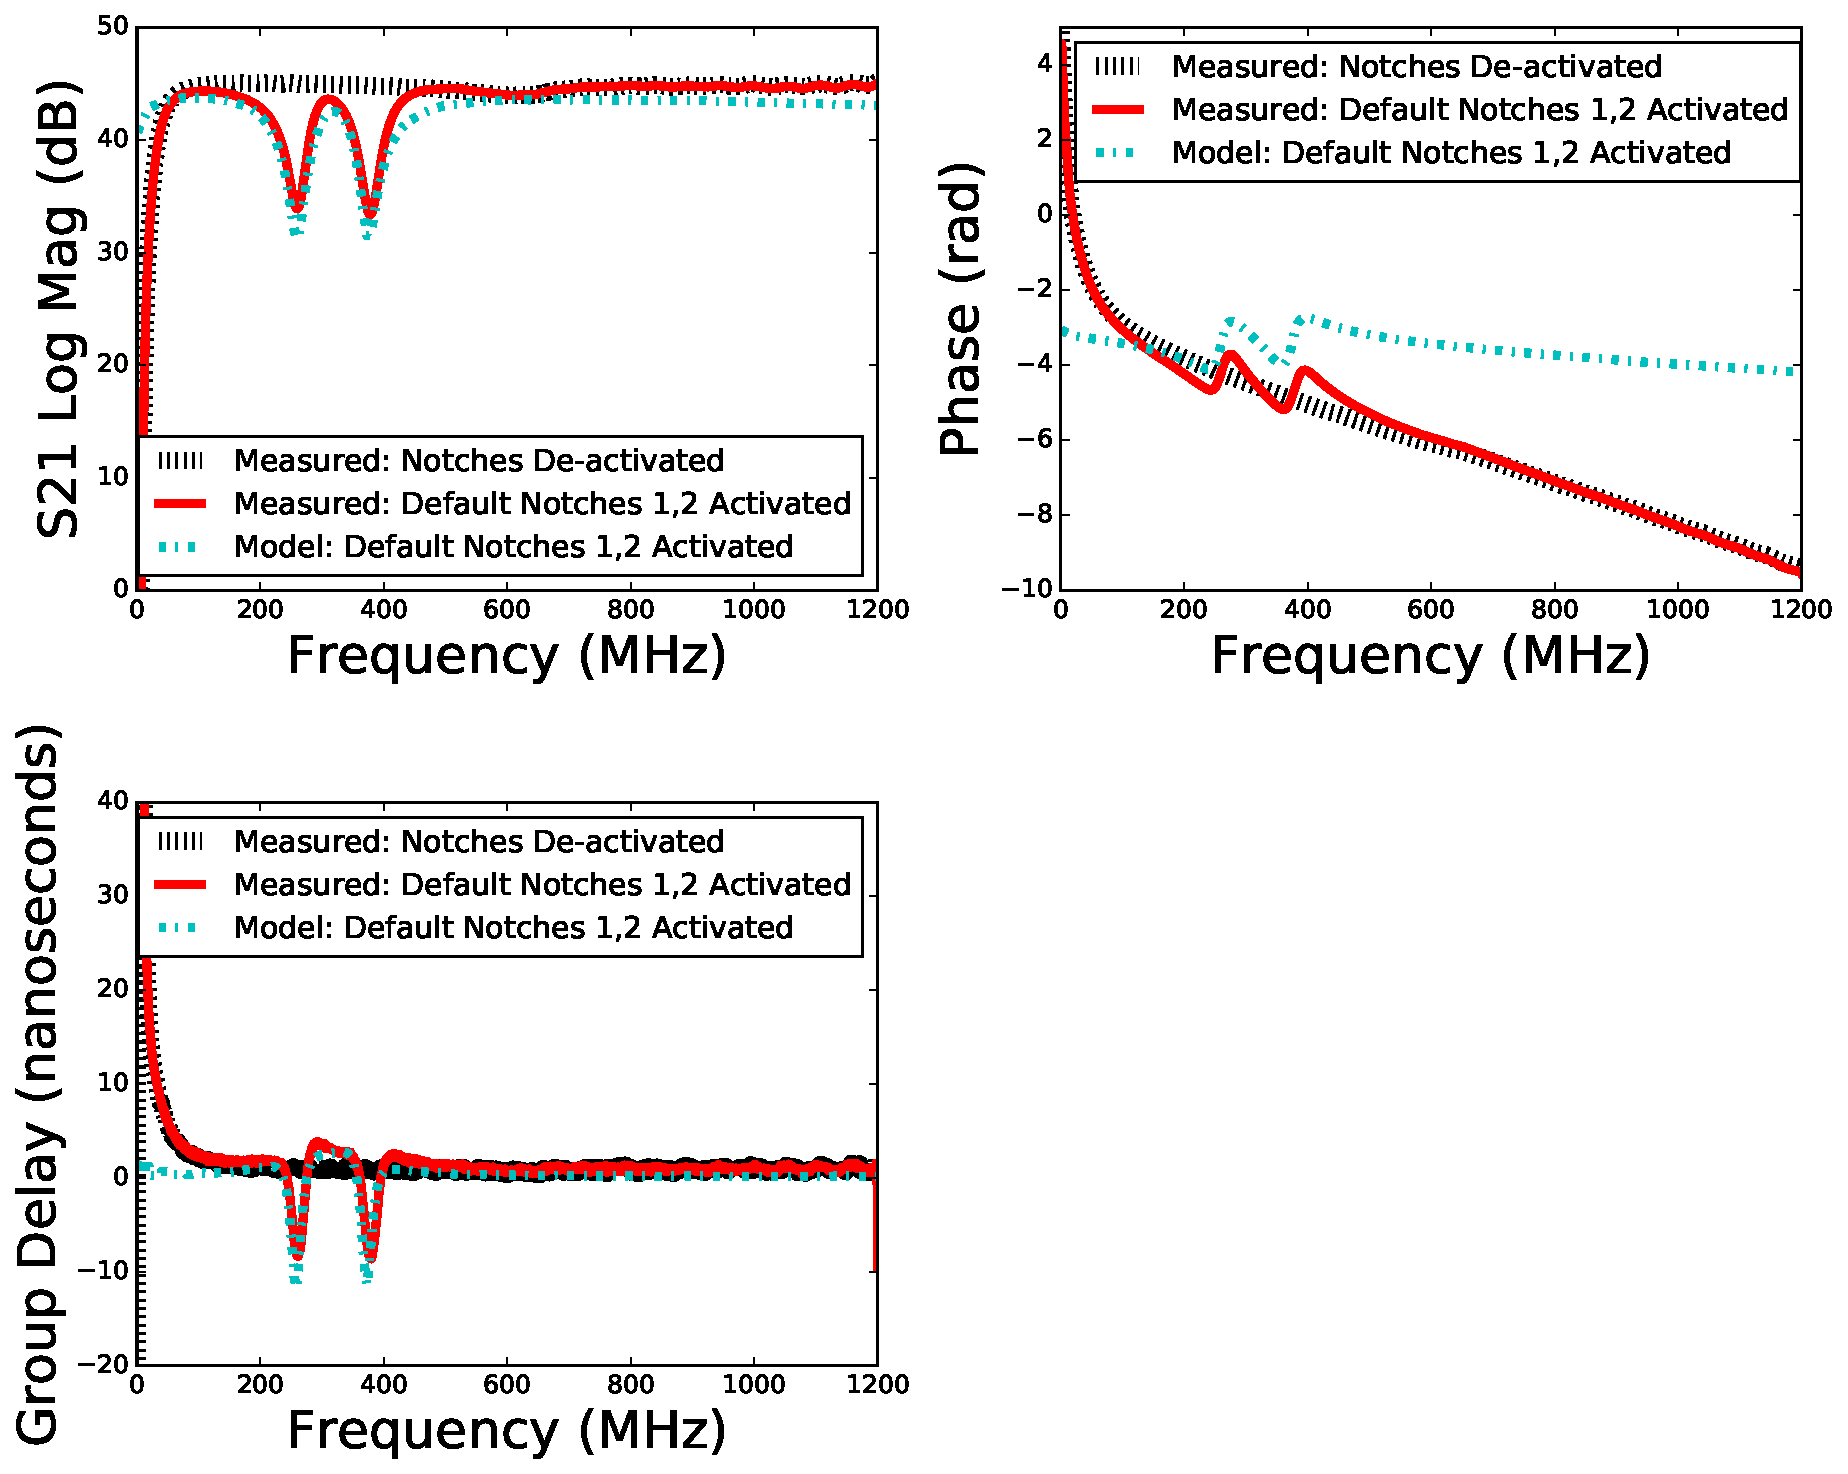
\includegraphics[width=1.0\textwidth]{figures/12measured_model_gain_phase_gd.pdf}
\caption{The gain, phase and group delay as measured and simulated for a TUFF channel with the first two notch filters activated (most common configuration used during the ANITA-4 flight) and all notch filters de-activated.}
\label{tuff_measured_model}
\end{figure}

\subsection{Microcontroller}

We use an ultra-low-power microcontroller, specifically a MSP430G2102 by Texas Instruments.
This features a powerful 16-bit Reduced Instruction Set Computing (RISC) central processing unit (CPU). 
There are five low-power modes optimized for extended battery life. 
The active mode consumes $220\,\mu\mbox{A}$ at $1\,\mbox{MHz}$ and $2.2\,\mathrm{V}$. 
The standby mode consumes only $0.5\,\mu\mbox{A}$ and the RAM retention-off mode consumes $0.1\,\mu\mbox{A}$.
The digitally-controlled oscillator allows wake-up from low-power modes to active mode in less than 
$1\,\mu\mbox{s}$. 

During the ANITA-4 flight, commands could be sent using the SIP connection to set the 
state of the variable capacitor of each \gls{tuff} notch filter via the microcontroller 
of that channel. 
This was done in real time if a re-tune of a notch filter was necessary to mitigate CW interference.
Commands could be sent to de-activate or activate a notch filter using the switch associated with each notch. 
Each microcontroller has the capability to communicate over universal serial communication interface.


\section{Impact of the TUFF boards}

The \gls{tuff} boards had a large impact on the livetime of \gls{anita}. 
There are two types of livetime in ANITA, which are described below.

\paragraph{Digitization livetime} 

In \gls{anita}, deadtime due to digitization by all four \gls{lab} chips of the SURF board is recorded by 
the TURF board, as illustrated in Figure~\ref{system}. 
This deadtime is recorded as a fraction of a second. Digitization livetime per second can be 
obtained by subtracting this from one. 
Increasing the digitization livetime increases the probability of receiving \gls{rf} signal due to an \gls{uhe} neutrino. 

\paragraph{Instrument livetime} 

At any given time, the digitization livetime multiplied by the fraction of unmasked phi sectors (after accounting for channel-masking) gives us the instrument livetime per second. 
In other words, instrument livetime accounts for the fraction of observable ice in azimuth after accounting for masking. 

\subsection{3x instrument livetime}

The most significant impact of the \gls{tuff} boards was the great reduction in the need for masking to mitigate noise during the \gls{anita}-4 flight as compared to \gls{anita}-3. This can be seen in Figure~\ref{masking}. The striking reduction in masking and increase in digitization livetime, as a result of implementing the \gls{tuff} notch filters, contributed to over 91.3\% instrument livetime in \gls{anita}-4 compared to the 31.6\% in \gls{anita}-3.
The performance and impact of the \gls{tuff} boards are described in detail in ~\cite{tuff}, along with visuals comparing the digitization and instrument livetime, thresholds and masking in \gls{anita}-3 and \gls{anita}-4. 

\begin{figure}
\centering
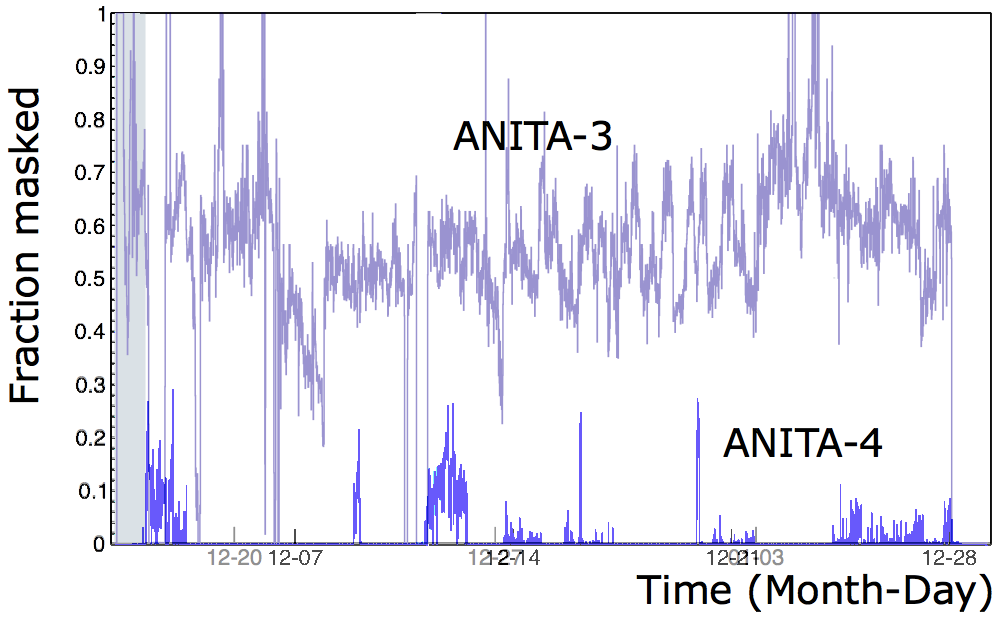
\includegraphics[width=1.0\textwidth]{figures/masking_compare.png}
\caption{Fractional masking implemented in the ANITA-4 and ANITA-3 (faded) flights as a function of time. The TUFF notch filters helped to reduce the need for masking and thereby, tripled the instrument livetime of the experiment.}
\label{masking}
\end{figure}

\begin{figure}
\centering
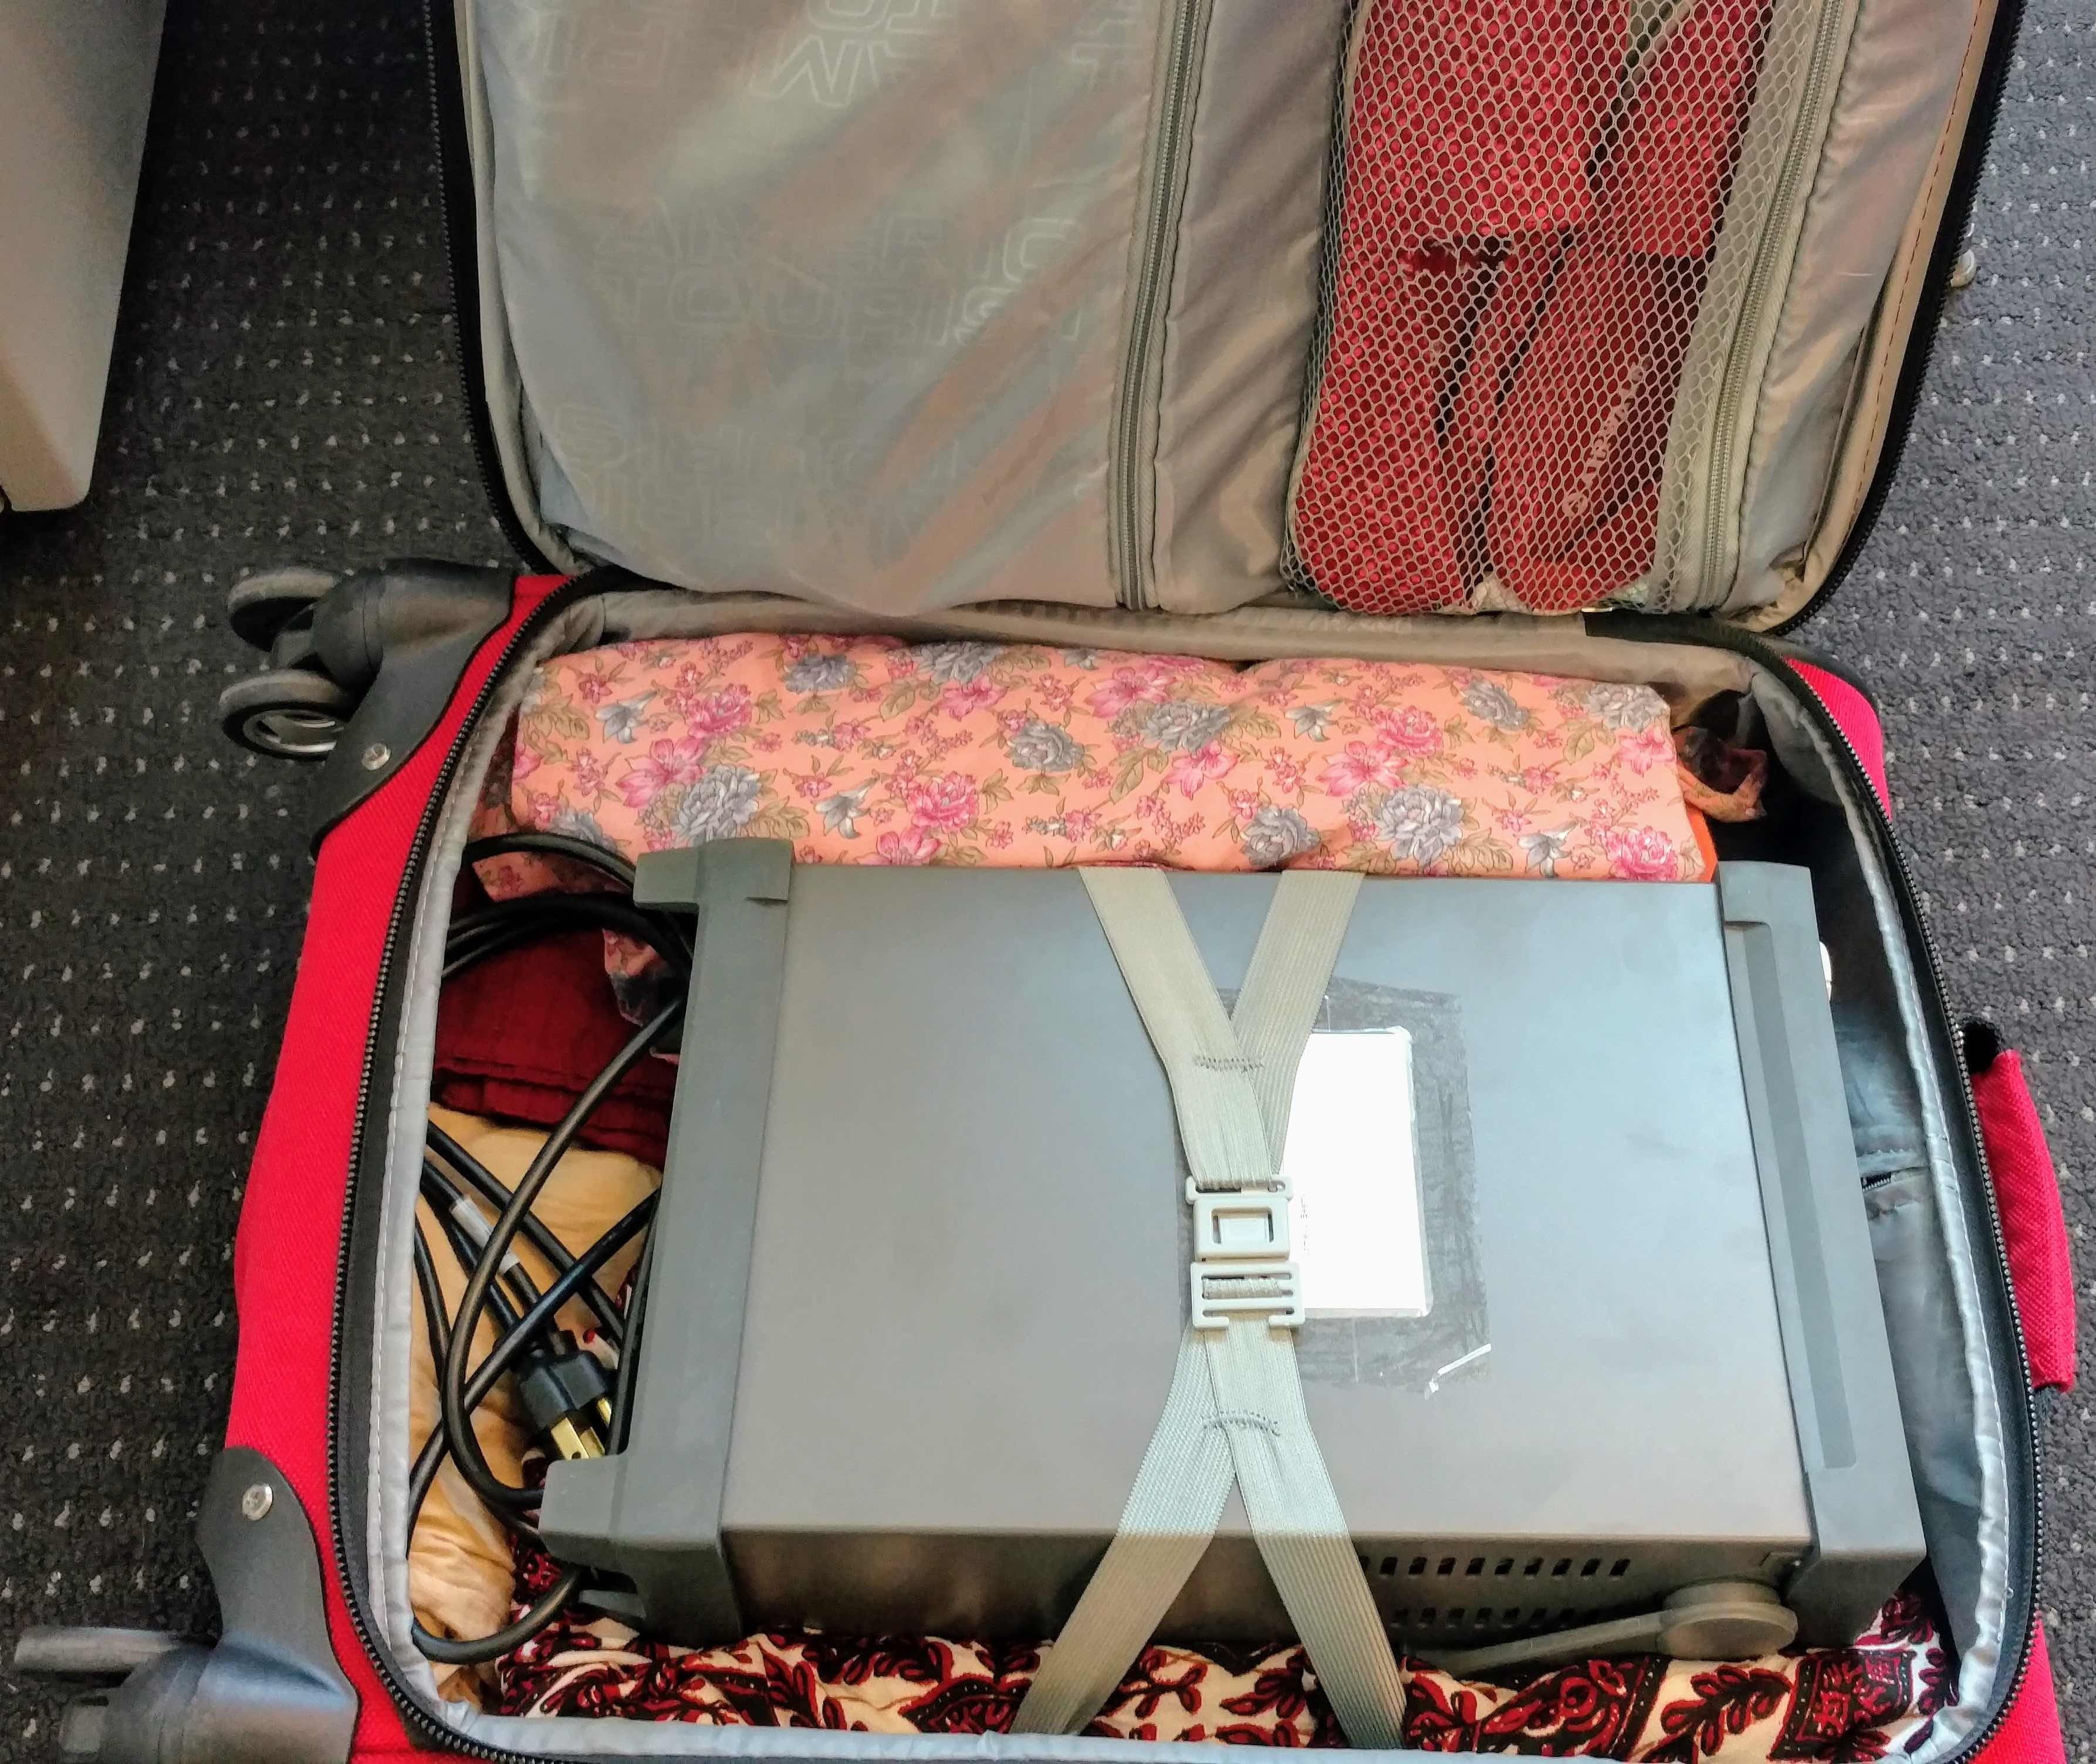
\includegraphics[width=1.0\textwidth]{figures/bag_for_palestine.jpg}
\caption{Bonus: This is the bag I packed for my trip to Palestine, TX, for the hang test of ANITA-4. I packed my own power supply. TUFF boards needed to be tested in Palestine for the integration and hang test, and they needed power. I thought it pertinent to carry my own as other folks' power supplies simply cannot be trusted, especially in challenging situations. This is from Jim Beatty's stash of lab equipment that he may let you borrow for such occasions. The highlight is I got this through airport security by telling the officers all about ANITA!}
\label{palestine_bag}
\end{figure}
\chapter{XUV Light Source Design and Apparatus Performance}

\section{Flux Requirements for ATAS Experiments}

copy this from the supplemental candidacy chapter.

\section{HHG Gas Source}

Transient absorption experiments require a high XUV photon flux for a variety of reasons. First, the sample thickness is usually chosen such that the XUV transmission is roughly 50\% near the spectral feature of interest. This optical density represents a compromise between the incompatible goals of having a strong ground state absorption (which allows you to easily detect small changes in optical density) while simultaneously avoiding the noise floor of the detector (which is required for good statistics). As a result, half of the XUV photons will never reach the detector, so you better be making a lot of them. Second, a high XUV flux will reduce the number of laser shots required for a given data point, which in turn reduces the chances of inadvertently damaging your sample with the infrared laser. Finally, a high flux reduces the overall time required to complete an experiment. Besides the obvious benefit of happier graduate students, the ability to quickly perform an experiment increases data fidelity by reducing the effects of unavoidable experimental noise sources such as long-term laser drift (either pointing or energy) or environmental changes caused by the building's HVAC system.

Depending on the energy of the spectral feature, obtaining a high photon flux can range from trivial to challenging. There are many (usually interdependent) experimental parameters (gas type, interaction pressure and length, wavelength, intensity, confocal parameter, focal position relative to gas source, etc.) that can be tuned to optimize photon flux. Physically, these parameters can change the microscopic single atom response, the macroscopic coherent addition of dipole emitters (via phase matching), or both. Each experiment will usually require a unique combination of experimental settings to achieve a usable light source. For example, optimizing the harmonic yield at 100 eV for a Si L-edge measurement will usually come at the expense of harmonics yield in the 30-50 eV range, which are used to measure the transition metal M-edges.

In general, an experimentalist has neither perfect knowledge nor control over all the variables that contribute towards phase matching. Setting aside the complicated topic of phase matching, the one dimensional on-axis phase matching model\cite{constantOptimizingHighHarmonic1999} shows that the photon flux is proportional to the square of the pressure-length product of the interaction gas. That is, so long as we can remain phase matched and below the critical phase matching pressure\cite{popmintchevPhaseMatchingHigh2009}, we can universally increase the harmonic flux of our experiments by increasing the pressure-length product.

Unfortunately, one cannot ignore phase matching. Oftentimes, the spectral feature of interest lies beyond the harmonic cutoff when using the more convenient shorter wavelengths. In this case, the fundamental wavelength is increased to extend the cutoff (which scales as $\lambda^2$). However, the critical phase matching pressure also scales as $\lambda^2$ \cite{popmintchevPhaseMatchingHigh2009}, and the single atom response scales as $\lambda^{-(5-6)}$ \cite{tateScalingWavePacketDynamics2007}. These two combined effects result in a dramatically decreased photon flux if intensity and pressure are kept constant with increasing wavelength, often to the point that the resulting flux is insufficient for a transient absorption experiment, even though your cutoff has been extended to the proper energy. While some of the flux can be recovered by increasing the backing pressure of the continuous free expansion nozzle, the generation chamber's finite pumping speed limits the efficacy of pressure tuning at the longer wavelengths. Even at 800 nm, the maximum backing pressure of the continuous free expansion nozzle results in an interaction pressure below the critical phase matching pressure. Practically speaking, the continuous free expansion gas nozzle is not suitable for transient absorption experiments using the signal wavelengths ($\lambda > 1.6 \ \mu m$) or with spectral features greater than the aluminum edge at 72 eV.

Providing the lab with a brighter harmonic source was the ultimate goal of the high pressure cell, and for the most part this goal was achieved. Below, we will review the basic design considerations, drawbacks and advantages of the three main types of gas sources used in this thesis: the free expansion nozzle, the low pressure cell and the high pressure cell. A primer on how to install and use the high pressure cell can be found in Appendix \ref{appendix:TABLe_manual}.

\subsection{Continuous Free Expansion Nozzle}
%outline of gas jet physics:
%- why supersonic? basic physics argument
%- outline of derivation to get to the T/P/rho relationships
%- outline of derivation to get to the centerline equations
%- mach disk location, description, thickness
%- derivation of gas nozzle throughput T
%
\begin{figure}
	\centering
	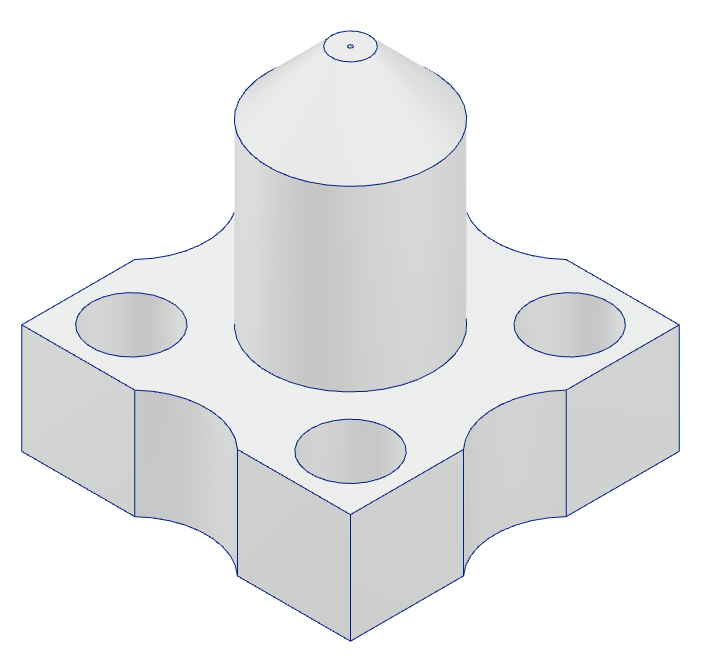
\includegraphics[width=0.5\textwidth]{figures/chap2/gas_nozzle.png}
	\caption{The continuous free expansion nozzle. Gas flows from the base of the nozzle and out of the 200 $\mu$m aperture. The large through holes on the base of the nozzle are for mounting to the gas delivery system; the sidewall cuts are for clearance for other mounting hardware. The top surface is beveled to reduce the minimum allowable distance between the laser axis and the nozzle.}
	\label{fig:gas_nozzle}
\end{figure}

\begin{figure}
	\centering
	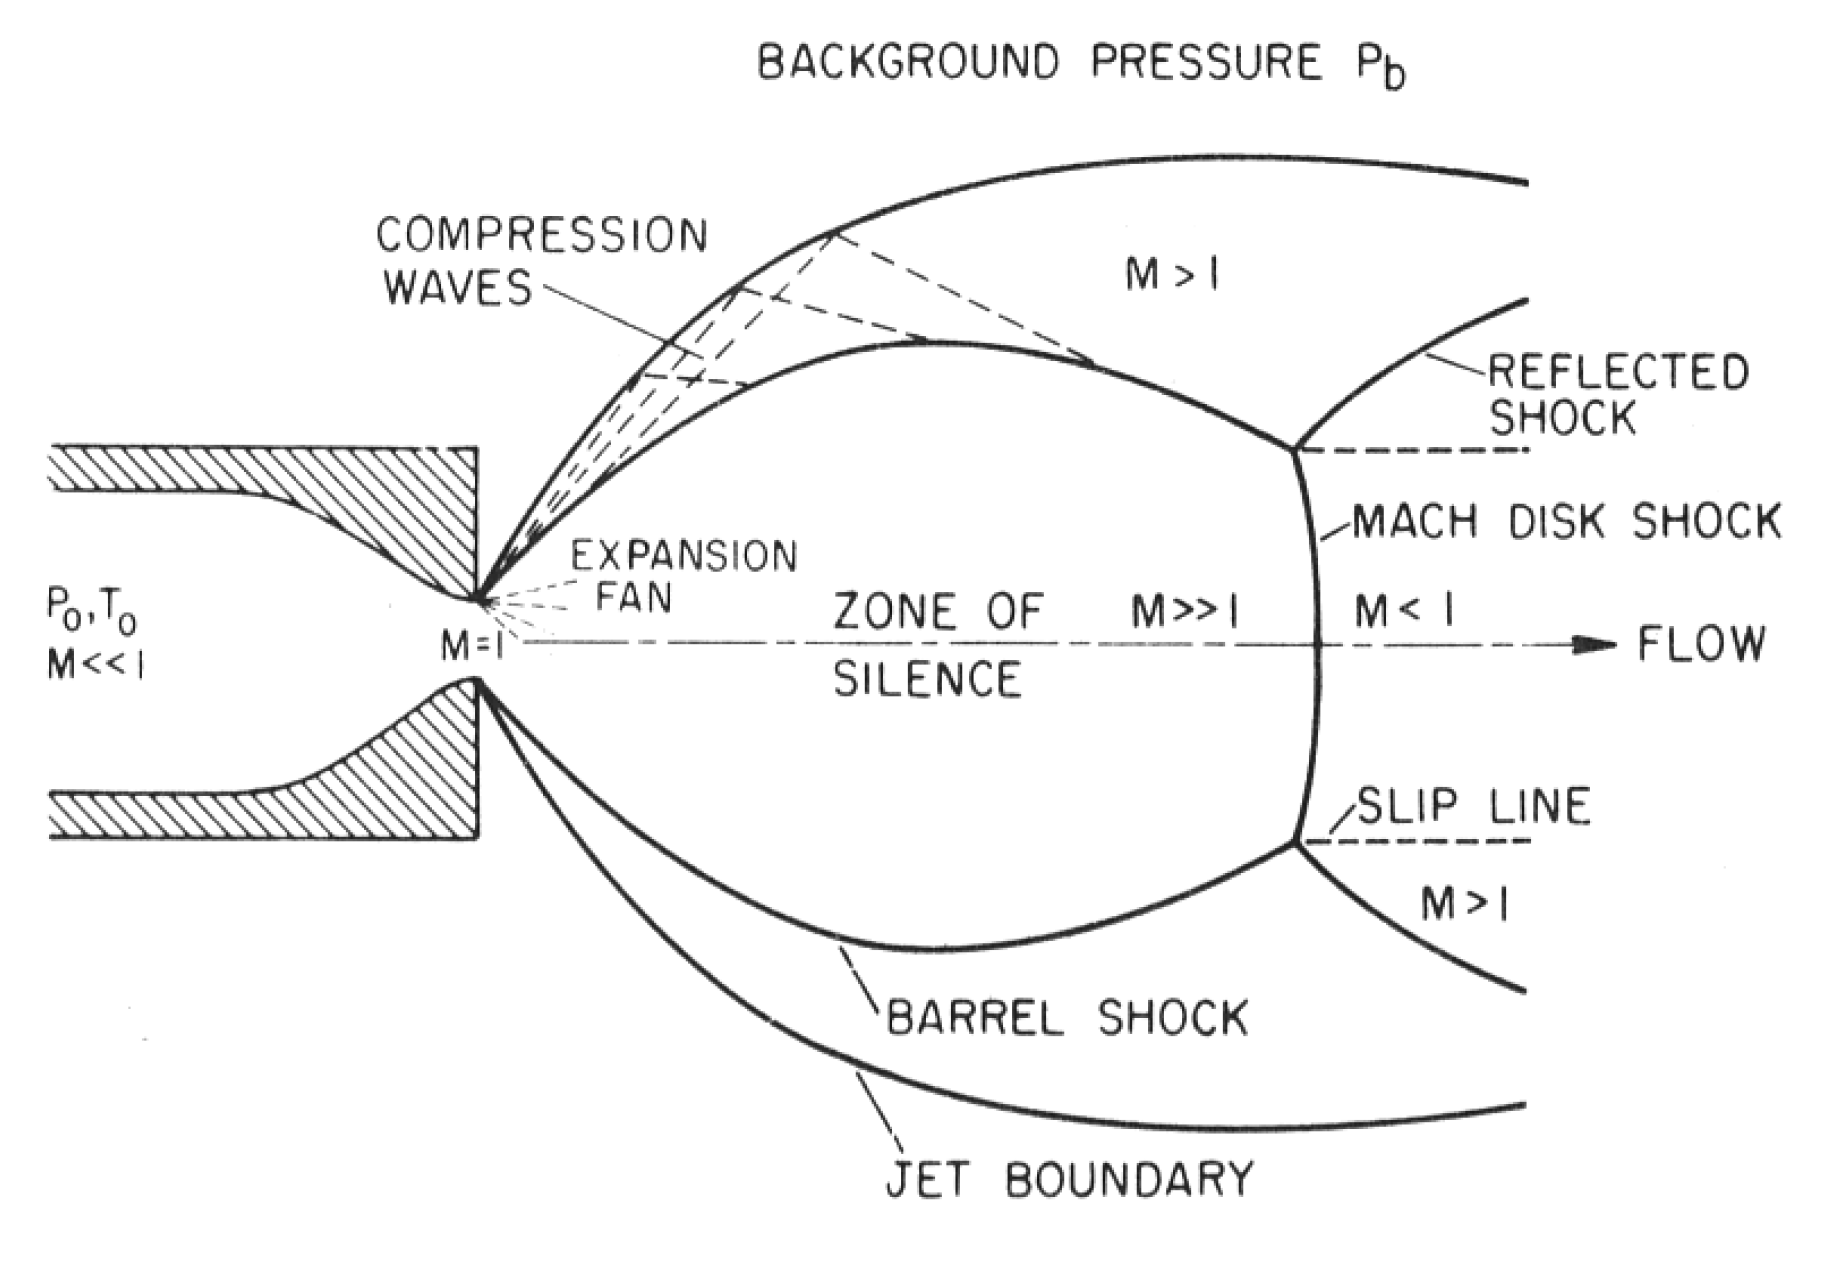
\includegraphics[width=0.5\textwidth]{figures/chap2/gas_expansion.PNG}
	\caption{The structure of the supersonic gas plume after leaving a gas nozzle. This figure was taken from Ref \cite{millerFreeJetSources1988}.}
	\label{fig:gas_expansion}
\end{figure}

\begin{figure}
	\centering
	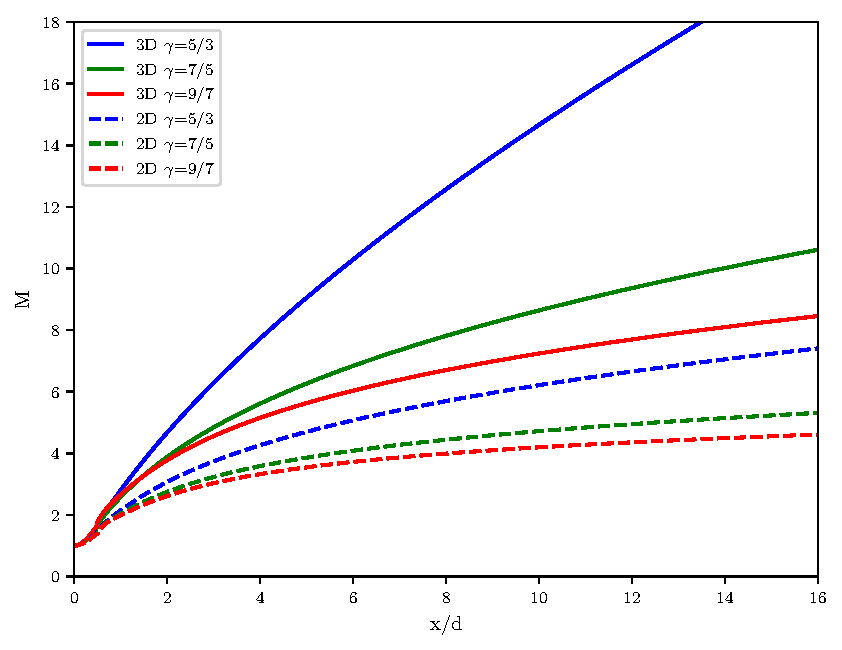
\includegraphics{figures/chap2/Scoles_Fig25.pdf}
	\caption{Centerline Mach number versus distance in nozzle diameters for 2D (planar) and 3D (axisymmetric) geometries, calculated using \cref{eqn:Scoles_centerline2.2}.}
	\label{fig:scoles_mach}
\end{figure}

\begin{figure}
	\centering
	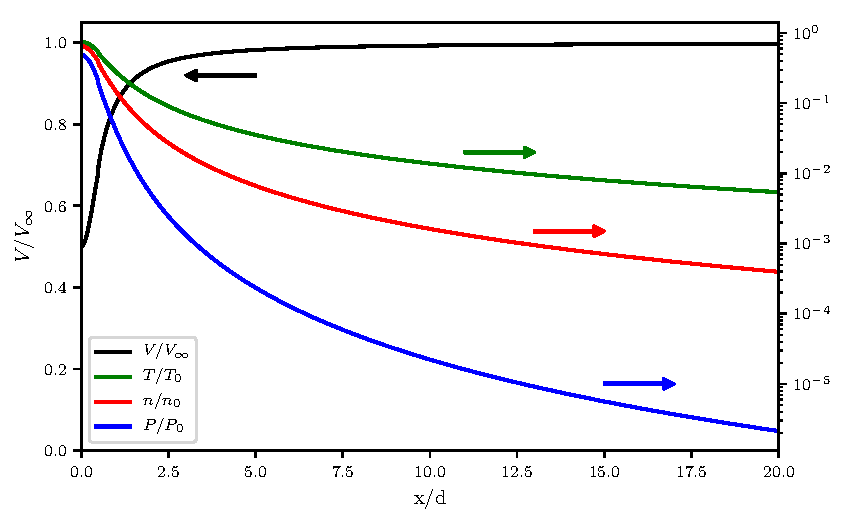
\includegraphics{figures/chap2/Scoles_Fig23.pdf}
	\caption{Free jet centerline properties versus distance in nozzle diameters for helium gas ($\gamma$=5/3, W=4). Mach number is calculated using \cref{eqn:Scoles_centerline2.2}, and the centerline properties are calculated using \cref{eqn:mach_properties}. Velocity $V$ is scaled by terminal velocity $V_{\infty}$; temperature $T$, number density $n$ and pressure $P$ are normalized by source stagnation values $T_0$, $n_0$, $P_0$.}
	\label{fig:scoles_centerline}
\end{figure}

When gas flows from a high pressure region ($P_0$) to a low pressure region ($P_b$) through a small aperture, a plume will form in the low pressure region. If the pressure ratio $P_0/P_b$ exceeds a critical value $G \equiv ((\gamma+1)/2)^{\gamma/(\gamma-1)}$, then the gas flow may exceed the local speed of sound. This critical value is at most 2.1 for all gases, so we easily exceed it in all of our experiments.\footnote{The highest chamber pressures in our experiments are on the order of $P_b \approx 10$ mTorr. Therefore, any nozzle that is backed by more than $P_0 \approx 21$ mTorr will result in a supersonic gas flow. Typical backing pressures for harmonic generation are on the order of 250 Torr, putting us well within the supersonic regime.} It is therefore necessary to understand the basic properties of supersonic gas plumes.

The continuous free expansion nozzle consists of a small diameter hole drilled in a block of aluminum, shaped to be convenient for gas delivery and assembly.\footnote{To reduce the gas load on the pumps, we used $200 \ \mu m$ diameter nozzles. This was the smallest size hole the machine shop could readily drill into aluminum.} The basic design is shown in \cref{fig:gas_nozzle}. The structure of the resulting supersonic plume is shown in \cref{fig:gas_expansion}. The physics of supersonic gas flow has been extensively studied in the literature and will not be discussed at length here. Below is a brief overview of the relevant physics required to understand the gas nozzles used for HHG in our lab. For a more detailed review of the field, see Ref \cite{millerFreeJetSources1988}.

% derivation of \cref{eqn:gas_dens}
energy equation. $V$ is velocity, $h$ is enthalpy per unit mass.
\begin{equation}
h + V^2/2 = h_0
\end{equation}
for ideal gases, $dh = \hat{C}_p \ dt$, and we have

\begin{equation}
V^2 = 2(h_0 -h) = 2 \int_{T}^{T_0} \hat{C}_p \ dT
\label{eqn:Scoles_gas_jet_energy}
\end{equation}

For an ideal gas, $\hat{C}_p = \gamma / (\gamma-1) (R/W)$, where $\gamma = C_p/C_V$ is the ratio of the specific heats, $R$ is the gas constant, $W$ is the molecular weight. if the gas is cooled substantially in the expansion ($T \ll T_0$), then we have:

\begin{equation}
V_{\infty} = \sqrt{ \frac{2R}{W} \left( \frac{\gamma}{\gamma-1} \right) T_0 }
\end{equation}

For an ideal gas, the speed of sound is $a = \sqrt{\gamma R T/W}$ and the Mach number is $M = V/a$. Assuming $\hat{C}_p$ is constant, we can recast \cref{eqn:Scoles_gas_jet_energy} in terms of $\gamma$ and $M$.  Using these assumptions, one can obtain the following relationships for the temperature $T$, velocity $V$, pressure $P$, mass density $\rho$ and number density $n$ in the gas jet scaled to those parameters at the stagnation point $(T_0, P_0, \rho_0, n_0)$:

\begin{subequations}
	\label{eqn:mach_properties}
	\begin{align}
	% eqn 2.3 - 2.6 in scoles, page 18
	(T/T_0) &= \left(  1 + \frac{\gamma-1}{2} M^2 \right)^{-1} \label{eqn:gas_temp} \\
	V &= M \sqrt{ \frac{\gamma R T_0}{W} } \left( 1 + \frac{\gamma-1}{2} M^2 \right)^{-1/2} \label{eqn:gas_velo} \\
	(P/P_0) &= (T/T_0)^{\gamma/(\gamma-1)} = \left(  1 + \frac{\gamma-1}{2} M^2 \right)^{-\gamma/(\gamma-1)} \label{eqn:gas_pres} \\
	(\rho/\rho_0) &= (n/n_0) = (T/T_0)^{1/(\gamma-1)} = \left(  1 + \frac{\gamma-1}{2} M^2 \right)^{-1/(\gamma-1)} \label{eqn:gas_dens}
	\end{align}
\end{subequations}

Therefore, once we know the Mach number $M$, we can calculate the above properties for the gas jet. The Mach number is found by solving the fluid mechanics equations dealing with the conversation of mass, momentum and energy:

\begin{subequations}
	\label{eqn:scoles_continuum}
	\begin{flalign}
	% eqn 2.7 of scoles, page 19
	\text{mass:} && \nabla \cdot (\rho \mathbf{V}) &= 0 && \label{eqn:scoles_mass} \\
	\text{momentum:} && \rho \mathbf{V} \cdot \nabla \mathbf{V} &= - \nabla P  && \label{eqn:scoles_momentum} \\
	\text{energy:} && \mathbf{V} \cdot \nabla h_0 &= 0 \textrm{ or } h_0 = \textrm{constant along streamlines} \label{eqn:scoles_energy} && \\
	\text{equation of state:} && P &= \rho \frac{R}{W} T  && \label{eqn:scoles_eqn-state} \\
	\text{thermal equation of state:} && dh &= \hat{C}_P \ dT \label{eqn:scoles_thermal-eqn-state} && 
	\end{flalign}
\end{subequations}

The above equations are valid for an isentropic, compressible flow of a single component ideal gas molecular weight $W$ and constant specific heat ratio $\gamma$. A steady state is assumed and viscosity and heat conduction are neglected. These equations have been numerically solved in the literature for two source geometries: a ``slit" nozzle (2D, planar) and a circular aperture (3D, axisymmetric). The numerical solutions to each geometry scale with the nozzle diameter $d$, and have been fit to the following analytical functions:

\begin{subequations}
	\label{eqn:Scoles_centerline2.2}
	\begin{align}
	% eqns from table 2.2 of scoles, page 23
	\frac{x}{d} > 0.5&: &&M = \left( \frac{x}{d} \right)^{(\gamma-1)/j} \left[ C_1 + \frac{C_2}{\left(\frac{x}{d}\right)} + \frac{C_3}{\left(\frac{x}{d}\right)^2} + \frac{C_4}{\left(\frac{x}{d}\right)^3} \right] \label{eqn:Scoles_centerline1} \\
	0 < \frac{x}{d} < 1.0&: &&M = 1.0 + A \left( \frac{x}{d} \right)^2 + B \left( \frac{x}{d} \right)^3 \label{eqn:Scoles_centerline2}
	\end{align}
\end{subequations}

\textbf{question: why does M increase without bound with increasing x, while V is limited to a finite value? scoles has a discussion, you should address it here.}

The fitting coefficients for \cref{eqn:Scoles_centerline2.2} are listed in \cref{tbl:Scoles_gas_params2.2}. A plot of the results for different source geometries and gases are shown in \cref{fig:scoles_mach}.


\begin{table}[]
	\centering
	\begin{tabular}{lllllllll}
		\hline
		\multicolumn{1}{c}{Source} & \multicolumn{1}{c}{$j$} & \multicolumn{1}{c}{$\gamma$} & \multicolumn{1}{c}{$C_1$} & \multicolumn{1}{c}{$C_2$} & \multicolumn{1}{c}{$C_3$} & \multicolumn{1}{c}{$C_4$} & \multicolumn{1}{c}{$A$} & \multicolumn{1}{c}{$B$} \\ \hline
		3D                         & 1                     & 5/3                          & 3.232                     & -0.7563                   & 0.3937                    & -0.0729                   & 3.337                & -1.541                \\
		3D                         & 1                     & 7/5                          & 3.606                     & -1.742                    & 0.9226                    & -0.2069                   & 3.190                 & -1.610                \\
		3D                         & 1                     & 9/7                          & 3.971                     & -2.327                    & 1.326                     & -0.311                    & 3.609                 & -1.950                \\
		2D                         & 2                     & 5/3                          & 3.038                     & -1.629                    & 0.9587                    & -0.2229                   & 2.339                 & -1.194                \\
		2D                         & 2                     & 7/5                          & 3.185                     & -2.195                    & 1.391                     & -0.3436                   & 2.261                 & -1.224                \\
		2D                         & 2                     & 9/7                          & 3.252                     & -2.473                    & 1.616                     & -0.4068                   & 2.219                 & -1.231               
	\end{tabular}
	\caption{Gas parameters used in free expansion calculations, with \cref{eqn:Scoles_centerline2.2}. Table recreated from Ref \cite{millerFreeJetSources1988}.}
	\label{tbl:Scoles_gas_params2.2}
\end{table}


\cref{tbl:Scoles_mach_params} shows the centerline Mach numbers used in the following equations:

\begin{subequations}
	\label{eqn:Scoles_centerline2.1}
	% eqns from table 2.1 of scoles, page 22
	\begin{align}
	M &= A \left( \frac{x-x_0}{d}\right)^{\gamma-1} - \frac{\frac{1}{2} \left( \frac{\gamma+1}{\gamma-1} \right)}{A \left(\frac{x-x_0}{d} \right)^{\gamma-1}} \label{eqn:gas_mach} \\
	\frac{\rho(y,x)}{\rho(0,x)} &= \cos^2(\theta) \cos^2\left(\frac{\pi\theta}{2\phi}\right) \\
	\frac{\rho(R,\theta)}{\rho(R,0)} &= \cos^2\left(\frac{\pi\theta}{2\phi}\right) \\
	\left(\frac{x}{d} \right) &> \left( \frac{x}{d} \right)_{\text{min}} \label{eqn:mach_cond}
	\end{align}
\end{subequations}
The gas nozzle throughput $\hat{T}$ is calculated from:


\begin{equation}
\hat{T} \ (\text{torr} \cdot \text{l}/\text{s}) = \hat{S} \cdot P_b = C \left(\frac{T_C}{T_0} \right)\sqrt{\frac{300}{T_0}}(P_0 d) d
\label{eqn:nozzle_thruput}
\end{equation}

where $C$ is the gas constant from \cref{tbl:Scoles_gas_params}, $P_0$ is the nozzle's backing pressure in Torr, $T_C$ and $T_0$ are the vacuum chamber and backing temperatures, respectively, in Kelvin, $P_0$ is the backing pressure in Torr, and $d$ is the nozzle's diameter in cm.

S = pumping speed?
Pb = chamber pressure

(how was this equation derived?)

Note that the gas nozzle throughput is proportional to both backing pressure and diameter of the nozzle. For our vacuum system, the generation chamber has a pumping speed of approximately ???; 

Relevant gas parameters are listed in \cref{tbl:Scoles_gas_params}.

condition for supersonic flow: the pressure ratio $P_0 / P_b$ exceeds a critical value $G \equiv ((\gamma+1)/2)^{\gamma/(\gamma-1)}$, which is less than 2.1 for all gases. Since the vacuum chamber pressure is at most 10 mTorr, just about any backing pressure will result in supersonic flow out of the gas nozzle.

Mach disk location: $x_M / d = 0.67(P_0/P_b)^{1/2}$. for example, for a chamber pressure of 10 mTorr and a backing pressure of -5 psig ($\sim$450 Torr), the Mach disk is located about 45 nozzle diameters away from the orifice. for a 200 micron diameter nozzle, that's about 9 cm.

\begin{table}[]
	\centering
	\begin{tabular}{llllll}
		Gas    & $\epsilon / k$ (K) & $\sigma$ (angstrom) & $C_6 / k$ ($10^{-43}$ K $\cdot$ cm$^6$) & $Z_r$     & \begin{tabular}[c]{@{}l@{}}C (l/cm$^2$/s);\\ \cref{eqn:nozzle_thruput}\end{tabular} \\ \hline
		He     & 10.9               & 2.66                & 0.154                                   & -         & 45                                                               \\
		Ne     & 43.8               & 2.75                & 0.758                                   & -         & 20                                                               \\
		Ar     & 144.4              & 3.33                & 7.88                                    & -         & 14                                                               \\
		Kr     & 190                & 3.59                & 16.3                                    & -         & 9.8                                                              \\
		Xe     & 163                & 4.3                 & 41.2                                    & -         & 7.9                                                              \\
		H$_2$  & 39.6               & 2.76                & 0.7                                     & $\sim$300 & 60-63                                                            \\
		D$_2$  & 35.2               & 2.95                & 0.93                                    & $\sim$200 & 42                                                               \\
		N$_2$  & 47.6               & 3.85                & 6.2                                     & $\sim$2.5 & 16                                                               \\
		CO     & 32.8               & 3.92                & 4.76                                    & $\sim$4.5 & 16                                                               \\
		CO$_2$ & 190                & 4.0                 & 31.1                                    & $\sim$2.5 & 12-13                                                            \\
		CH$_4$ & 148                & 3.81                & 18.1                                    & $\sim$15  & 21                                                               \\
		O$_2$  & 115                & 3.49                & 8.31                                    & $\sim$2   & 15                                                               \\
		F$_2$  & 121                & 3.6                 & 10.5                                    & $\sim$3.5 & 14                                                               \\
		I$_2$  & 550                & 4.98                & 336                                     & $\sim$1   & 5.2                                                              \\ \hline
	\end{tabular}
	\caption{Gas parameters used in free expansion calculations. Table recreated from Ref \cite{millerFreeJetSources1988}.}
	\label{tbl:Scoles_gas_params2.1}
\end{table}

\begin{table}[]
	\centering
	\begin{tabular}{lllll}
		\hline
		$\gamma$ & $x_0/d$ & $A$  & $\phi$ & $(x/d)_{\text{min}}$ \\ \hline
		1.67     & 0.075   & 3.26 & 1.365  & 2.5                  \\
		1.40     & 0.4     & 3.65 & 1.662  & 6                    \\
		1.2857   & 0.85    & 3.96 & 1.888  & 4                    \\
		1.20     & 1.00    & 4.29 & -      & -                    \\
		1.10     & 1.60    & 5.25 & -      & -                    \\
		1.05     & 1.80    & 6.44 & -      & -                    \\ \hline
	\end{tabular}
	\caption{Centerline Mach Number and Off-Axis Density Correlations for Axisymmetric Flow. Table recreated from Ref \cite{millerFreeJetSources1988}.}
	\label{tbl:Scoles_mach_params}
\end{table}

basic design of free expansion nozzle

throughput calculations (Scoles)

harmonic yield results

note: i did not design this cell

advantages: easy to align, cheap to produce, free-expansion cooling (for alignment experiments)

disadvantages: small pressure length product. very low interaction pressure. impossible to phase match longer wavelengths. overall low yield. 

\subsection{low pressure cell}

\begin{figure}
	\centering
	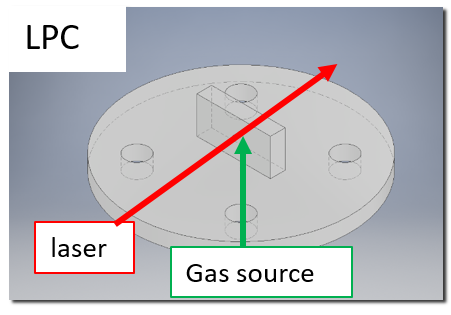
\includegraphics[width=0.5\textwidth]{figures/chap2/LPC_diagram.png}
	\caption{Detail of the LPC interaction region.}
	\label{fig:LPC_diagram}
\end{figure}

\begin{figure}
	\centering
	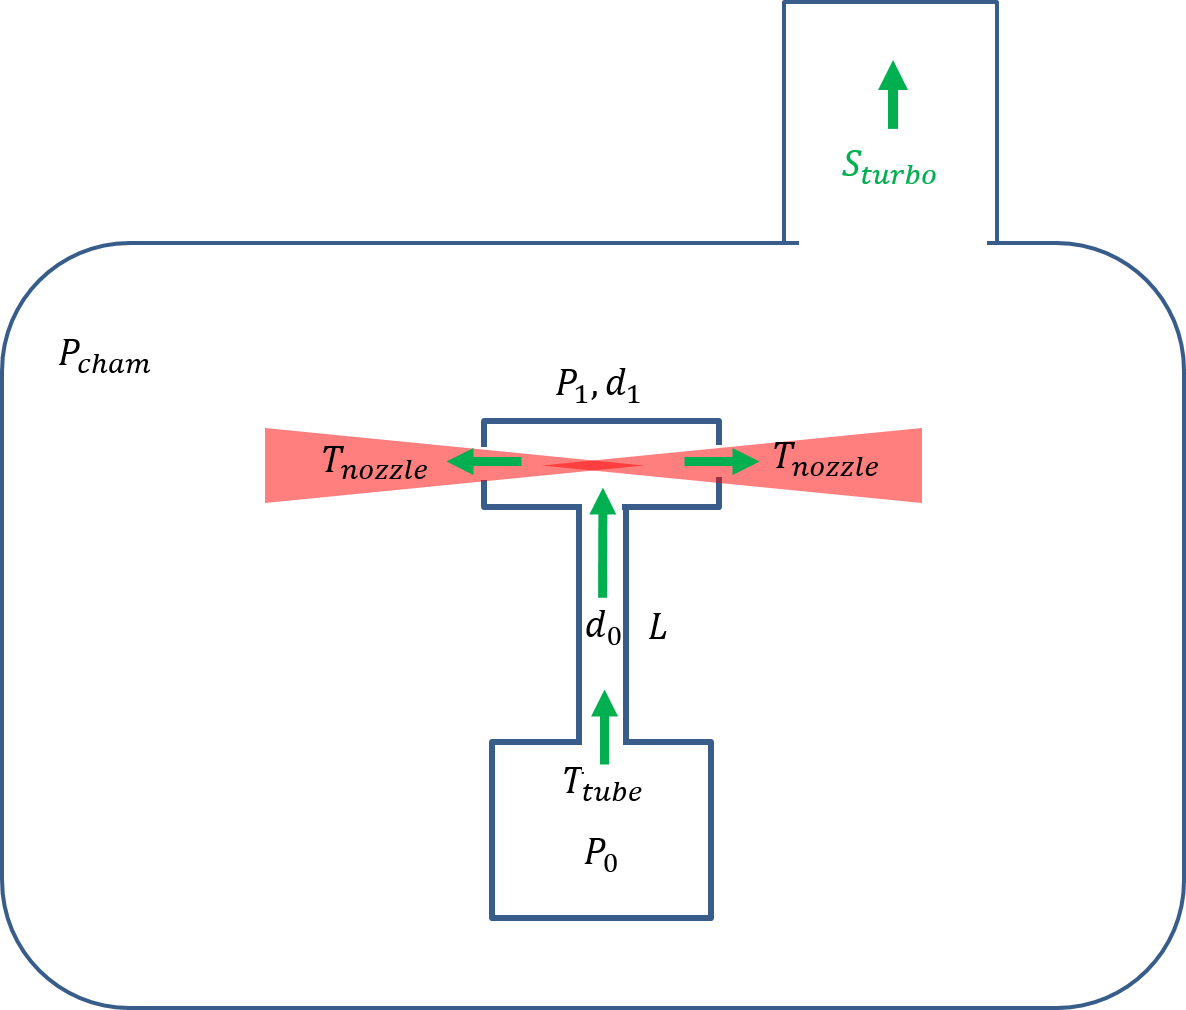
\includegraphics[width=0.75\textwidth]{figures/chap2/LPC_schematic2.png}
	\caption{Gas flow schematic of the LPC. The green arrows indicate the direction of gas flow, and the red shaded region indicates the laser path. An infinite reservoir of gas with backing pressure $P_0$ supplies the laser interaction region with gas via a thin capillary of diameter $d_0$, length $L$ and throughput $T_{tube}$. The interaction region has pressure $P_1$ and diameter $d_1$. The interaction region acts as a pressure source for two diametrically opposed supersonic gas jets, each with throughput $T_{nozzle}$. The generation chamber has a turbopump with pumping speed $S_{turbo}$ and an equilibrium pressure $P_{cham}$.}
	\label{fig:LPC_schematic}
\end{figure}

basic design of low pressure cell -- gas load, Rayleigh range, spot size, laser drift

gas load calculations (simple model)

harmonic yield results

note that i did not design this cell. design is from (now Dr.) Zhou Wang.

advantages: increased interaction length - brighter! easy to align.

disadvantages: relative to the free expansion nozzle, you don't get any cooling.

\subsection{high pressure cell}

\begin{figure}
	\centering
	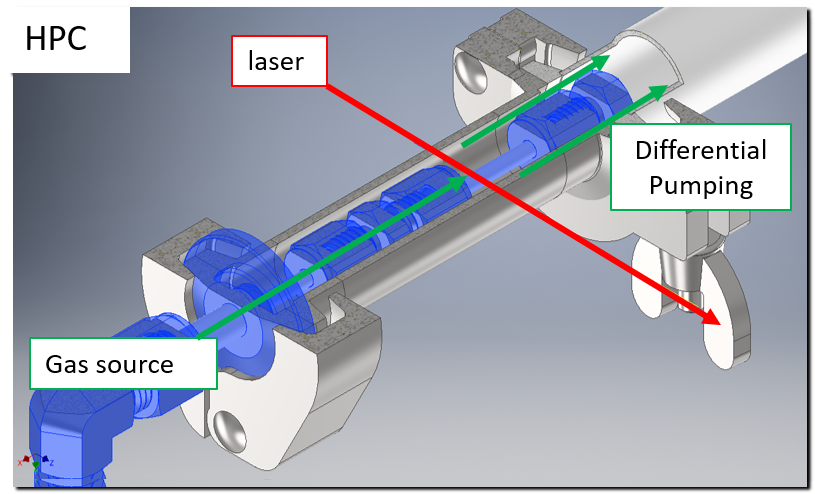
\includegraphics[width=0.9\textwidth]{figures/chap2/HPC_cutaway2.png}
	\caption{Detail of the HPC interaction region. From bottom left to top right: welded gas feedthrough, concentric inner \& outer pipes, edge-welded bellows. The high pressure region is shaded blue. The green lines indicate the gas flow direction; the red line indicates the laser propagation direction.}
	\label{fig:HPC_cutaway2}
\end{figure}

\begin{figure}
	\centering
	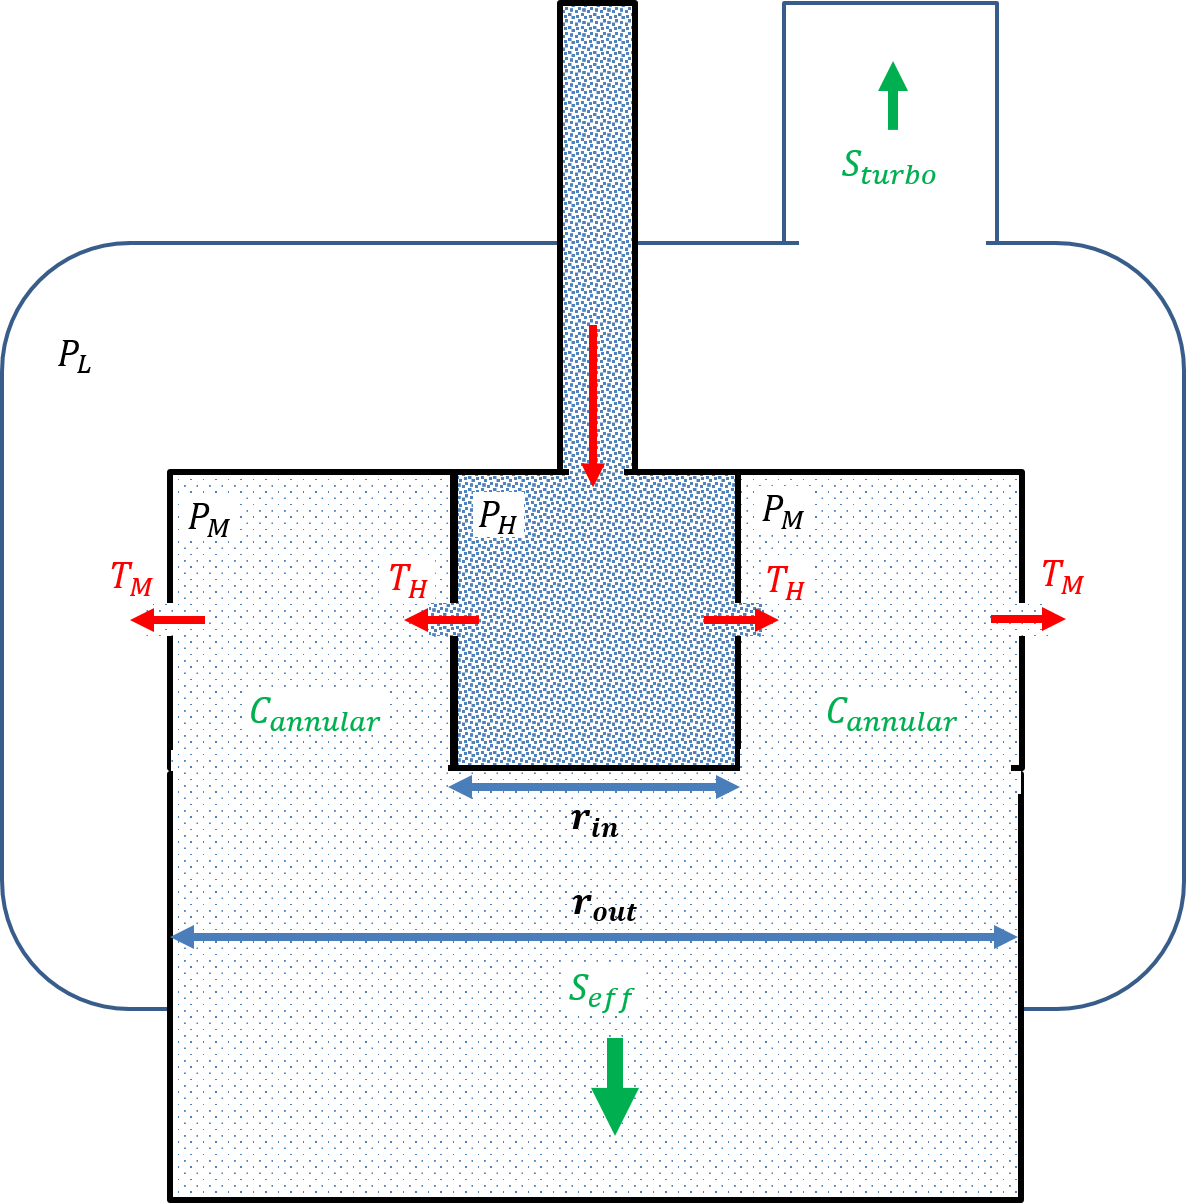
\includegraphics[width=0.9\textwidth]{figures/chap2/HPC_pressure_schematic.png}
	\caption{Schematic used to calculate the pressures inside the HPC and generation chamber. The dark blue region represents the inner pipe, the light blue region represents the outer pipe. Red arrows and text indicate gas sources, green arrows and text indicate flow towards the vacuum pumps; blue arrows and text indicate physical dimensions. $P_H$, $P_M$, and $P_L$ are the pressures of the inner pipe, outer pipe, and generation chamber, respectively; $S_{turbo}$, $S_{eff}$ and $C_{annular}$ are the turbo pumping speed, effective rough pumping speed and annular conductance, respectively; $T_H$ ($T_M$) is the gas throughput from the high (medium) pressure region into the medium (low) pressure region.}
	\label{fig:HPC_pressure_schematic}
\end{figure}

- why didn't you go with semi-infinite gas cell, or fiber-cell?

- basic design of high pressure cell

- limited pump speed $\rightarrow$ differential pumping is required

- gas load calculations (simple model)

harmonic yield results

advantages: much brighter due to pressure-length product. future application: can operate in low-pressure mode and reduce downstream generation gas contamination of target chamber.

disadvantages: difficult to align and initially install (once it's installed, alignment is easy). messed up mode. HHG instability at higher pressures.

\subsection{pulsed valve}

expensive





\section{Harmonic Gas Sources}

\subsection{free expansion gas jet nozzle}

\subsection{low pressure cell}

\subsection{high pressure cell}
\label{sec:HPC}

\subsection{amsterdam pulsed piezoelectric valve}

\section{characterization of XUV source}

\subsection{knife edge measurements at XUV focus}

\begin{figure}
	\centering
	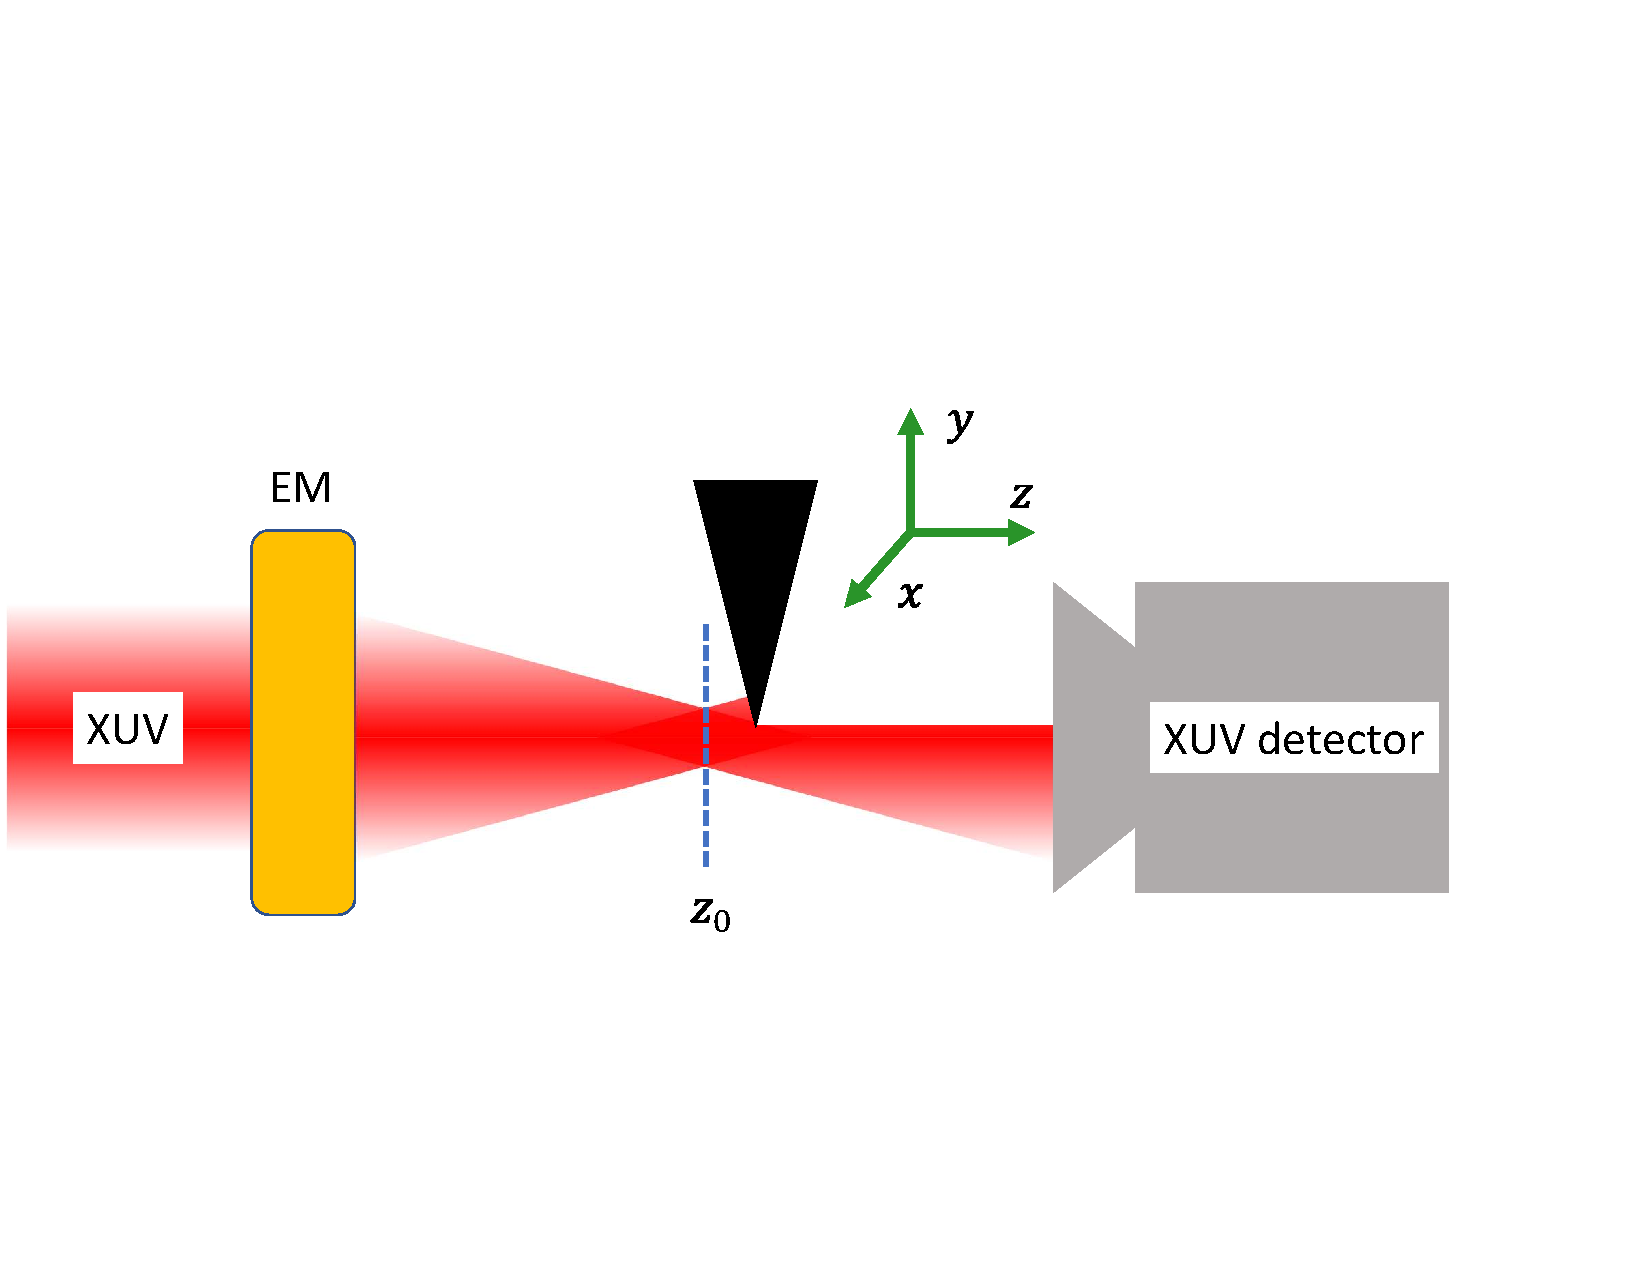
\includegraphics[width=0.75\textwidth]{figures/chap3/knife_edge_cartoon.pdf}
	\caption{Schematic of XUV knife edge measurement. EM: ellipsoidal mirror, $z_0$: XUV focal plane.}
	\label{fig:knife_edge_cartoon}
\end{figure}

\begin{figure}
	\centering
	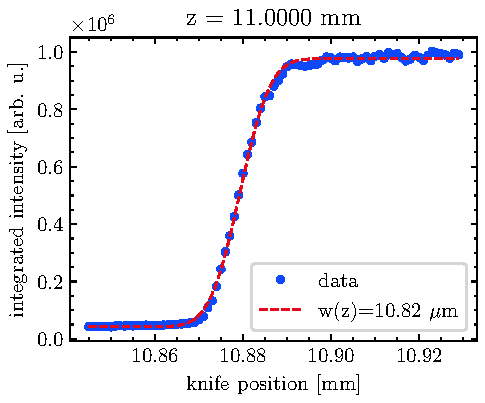
\includegraphics[width=0.75\textwidth]{figures/chap3/XUV_focus_knife_edge.pdf}
	\caption{A typical XUV knife edge measurement near the focal plane. The sample motor position is $k=11.0000$ mm. A fit to equation \cref{eqn:knife_edge} yields a beam waist of 10.82 $\mu$m at this position.}
	\label{fig:XUV_focus_knife_edge}
	% dataset: C:\testdata\2019_08_23\knife\11.0000
	% python file: \Python Scripts\Spectrometer\test\knife_edge.py
\end{figure}

\begin{figure}
	\centering
	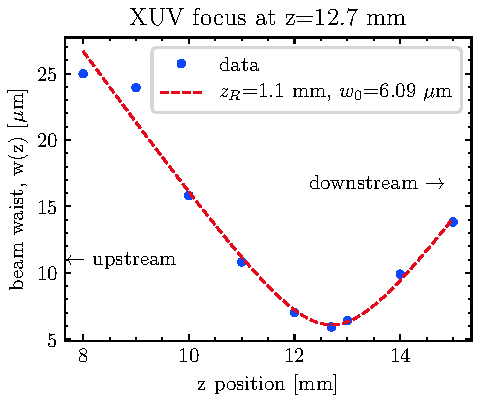
\includegraphics[width=0.75\textwidth]{figures/chap3/XUV_waist_vs_k.pdf}
	\caption{Evolution of XUV beam waist as a function of propagation direction, $z$. The Rayleigh range $z_R$ and beam waist $w_0$ are extracted from the fit to \cref{eqn:beam_waist_evolution}.}
	\label{fig:XUV_waist_vs_k}
	% question: what is $M^2$ value of the XUV?. or, does w0 and zR change with XUV wavelength?
	% dataset: C:\testdata\2019_08_23\knife\11.0000
	% python file: \Python Scripts\Spectrometer\test\knife_edge.py
\end{figure}

We characterize the XUV focus in the target chamber by performing knife edge measurements at different $k$-positions, as depicted in \cref{fig:knife_edge_cartoon}. We use the interior angled edge of the Si frame on a broken sample heterostructure as a knife edge (see \cref{fig:Sample_Geometry}). This frame makes an excellent knife edge as it has a very well-defined geometry and fits in the sample holder. Recalling Gaussian optics, the assumed profile of the XUV beam is:
\begin{equation}
I(x,y,z) = I_0 \left( \frac{w_0}{w(z)} \right)^2 \exp \left( - 2 ((x-x_0)^2 + (y-y_0)^2) /  w(z)^2 \right),
\end{equation}
using the coordinate system defined in \cref{fig:knife_edge_cartoon}. The XUV focus is at position $(x_0,y_0,z_0)$. The beam waist $w(z)$ will evolve as:
\begin{equation}
w(z) = w_0 \sqrt{ 1 + \left( \frac{z-z_0}{z_R} \right)^2 },
\label{eqn:beam_waist_evolution}
\end{equation}
where $z_R$ is the Rayleigh range. If we use the knife edge to block the transmission as depicted in \cref{fig:knife_edge_cartoon}, then the transmitted power will be:
\begin{equation}
P(x, z) = P_0 + \frac{P_{max}}{2} \left( 1 - \erf \left( \frac{\sqrt{2}(x-x_0)}{w(z)} \right) \right),
\label{eqn:knife_edge}
\end{equation}
where $x$ is the insertion of the knife in the beam, $z$ represents the location of the knife plane in the propagation direction, and $\erf$ is the error function.

A typical knife edge measurement is shown \cref{fig:XUV_focus_knife_edge}. In this measurement, the knife edge is translated across the XUV spot in 1 $\mu$m steps until the XUV light is completely blocked. A 2D spectrum is saved at each knife edge position. Each image is background subtracted, normalized and summed (integrating over all divergences and wavelengths), which yields the XUV flux as a function of knife position. The resulting curve is fit to \cref{eqn:knife_edge} and the beam waist $w(z)$ is extracted for this $z$-position.

The knife edge measurement is repeated at different $z$-positions until enough data has been acquired to determine the focal plane. The evolution of the XUV beam waist is shown in \cref{fig:XUV_waist_vs_k}. In this figure, the beam waist has been fit to \cref{eqn:beam_waist_evolution} to determine the focal plane $z_0$, the Rayleigh range $z_R$ and the beam waist $w_0$. In both figures, a reasonably good fit is obtained, indicating that the XUV light has a Gaussian spatial profile near the focus.


\subsection{harmonic yield stability}

\subsection{XUV spectra optimized for various HHG conditions}

\subsection{Measured Transmission of Metallic Filters}

\subsection{Ground State Measurements of Condensed Matter Samples}

\section{characterization of interferometric stability}

\section{MCP response}

scaling of yield and noise with respect to MCP voltage
\chapter{ATAS Experiments in Germanium}
\label{chap:ATAS_in_Ge}


\section{Introduction}







\begin{figure}
	\centering
	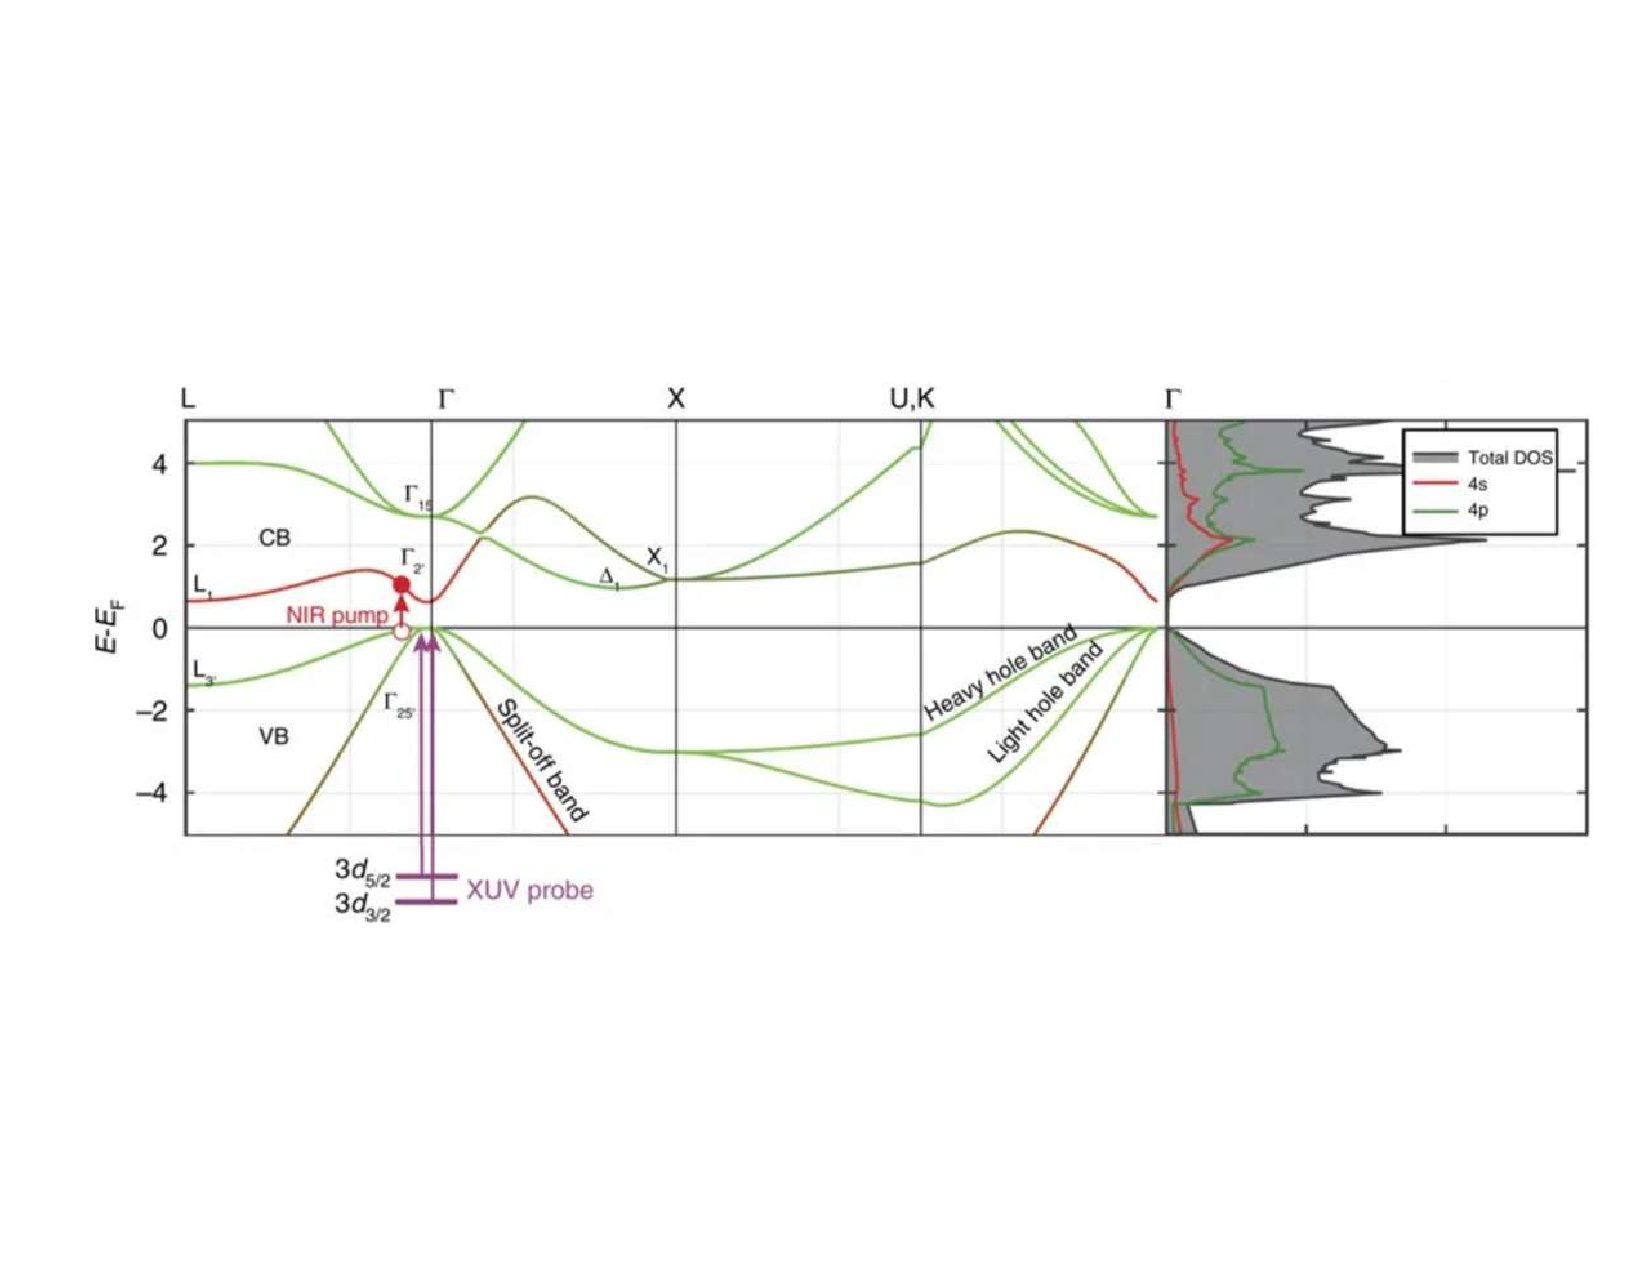
\includegraphics[width=0.75\textwidth]{figures/chap4/Ge_band_diagram_Zurch2017.pdf}
	\caption{Band structure and orbital character of germanium. Purple arrows indicate XUV-induced transitions from the $3d$ core levels to the valence bands. Red arrow indicates IR-induced transition across the direct band gap. Figure adapted from \cite{zurchDirectSimultaneousObservation2017}.}
	\label{fig:Ge_band_diagram}
\end{figure}

previous chapters: designed, built and tested a high-brightness XUV light source. haven't yet talked about the interferometer much? now, need to introduce the following concepts:
\begin{itemize}
	\item scientific motivation / goal for studying ATAS in condensed matter in general.
	\item general sample requirements (thickness, absorption edge)
	\item ground state measurements of various materials
	\item scientific motivation / goal for studying ATAS in germanium specifically.
	\item intensity / ionization inside germanium (TMM/Keldysh)
	\item experimental results of Ge ATAS

\end{itemize}

\section{Experimental Considerations}

\subsection{Sample Requirements}

\begin{figure}
	\centering
	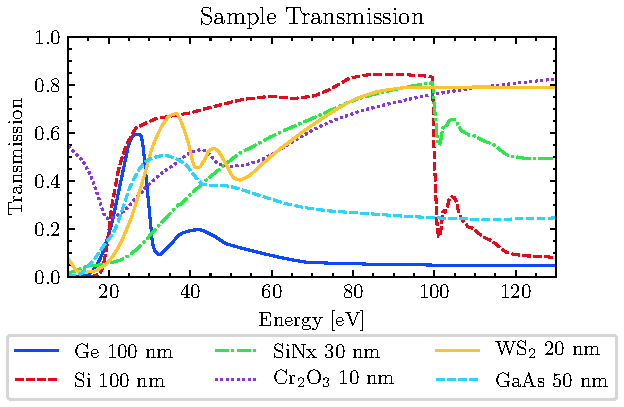
\includegraphics[width=0.75\textwidth]{figures/chap4/Sample_transmission_CXRO.pdf}
	\caption{Calculated XUV transmission of various materials. Data from \cite{gulliksonCXROXRayInteractions}.}
	\label{fig:Sample_trans_CXRO}
	% figure generated using \PythonScripts\CXRO\test\CXRO.py
\end{figure}

There are several sample requirements for a successful condensed matter transient absorption experiment. First and foremost, the sample needs to have an absorption edge within the bandwidth of the XUV source. Second, the material must be the correct thickness for a transmission measurement, given the capabilities of the XUV light source and detector. If the material is too thick, the ground state will absorb most of the XUV flux and the recorded spectrum will be too close to the noise floor of the apparatus. If it is too thin, insufficient XUV absorption will occur and the laser-induced change of the ground state (on the order of $1-10\%$) will be lost in the noise floor. As a general guideline, a sample that absorbs 50\% at the spectral feature of interest provides a good compromise between these conflicting requirements. \cref{fig:Sample_trans_CXRO} shows the expected transmission of several materials, calculated from the atomic scattering factors \cite{gulliksonCXROXRayInteractions}. We can see that a typical sample will be on the order of 10 - 200 nm thick, depending on the material.

Another upper bound for sample thickness comes from material dispersion. In any material, the XUV light ($n_{\text{XUV}} \sim 1$) will outpace the IR light ($n_{\text{IR}} > 1$). This effect can be significant even for ultrathin films. In order to keep the phase slippage between the XUV and IR light below half an IR period, the sample thickness $L$ must obey the following relationship:
\begin{equation}
L \le \frac{1}{2} \frac{\lambda_{\text{IR}}}{n_{\text{IR}} - n_{\text{XUV}}}
\end{equation}
For germanium excited with $\lambda_{\text{IR}}$ = 1430 nm and probed with 30 eV XUV at the $M_{4,5}$ edge, $n_{\text{IR}}$ = 4.2481 \cite{nunleyOpticalConstantsGermanium2016} and $n_{\text{XUV}}$ = 0.992536 \cite{gulliksonCXROXRayInteractions}, which gives a maximum thickness of 220 nm.

Next, the sample needs to be excitable using laser sources present in our lab (i.e., ultrafast pulses with wavelengths between 800 nm and a couple of microns). To minimize the slow build up of heat (on the order of seconds) and laser-induced damage, the sample needs to be rastered through the laser focus as the experiment is performed. This rastering method necessitates both a large clear aperture ($\sim$ 1 mm$^2$ - 1 cm$^2$) and good sample uniformity. Samples that meet the above thickness and clear aperture requirements are extremely delicate, with thicknesses between 5,000 and 100,000 times smaller than their freestanding lateral dimensions. As such, one should expect most samples to break before, during and after measurements, so a successful experiment will have a materials pipeline that is capable of producing multiple, consistent samples in a short time frame.

\subsection{Data Collection Sequence}

The absorbance $A$ is defined as the negative logarithm of the transmission $T$:
\begin{equation}
A(E) = -\log_{10}(T) = - \log_{10} \left( \frac{S_{\textrm{g.s.}}(E)}{S_{\textrm{vac.}}(E)} \right)
\label{eqn:def_absorbance}
\end{equation}
In \cref{eqn:def_absorbance}, $S_{\textrm{g.s.}}$ is the XUV spectrum transmitted by the sample in its ground state and $S_{\textrm{vac.}}$ is the spectrum without the sample present. Therefore we can measure the sample's ground state absorbance by measuring the harmonic spectrum with and without the sample in the XUV beam. The \textit{change in absorbance} $\Delta A$ between the ground and laser-induced state is therefore:
\begin{equation}
\begin{aligned}
\Delta A(E,\tau) &= A_{\textrm{e.s.}}(E) - A_{\textrm{g.s.}}(E)\\
&= - \log_{10} \left( \frac{S_{\textrm{e.s.}}}{S_{\textrm{vac.}}} \right) + \log_{10} \left( \frac{S_{\textrm{g.s.}}}{S_{\textrm{vac.}}} \right)\\
&= - \log_{10} \left( \frac{S_{\textrm{e.s.}}}{S_{\textrm{g.s.}}} \right)
\end{aligned}
\label{eqn:def_Delta_absorbance}
\end{equation}
In \cref{eqn:def_Delta_absorbance}, the signal spectrum $S_{\textrm{e.s.}}(E, \tau)$ is the spectra that results from an IR pulse hitting the sample, followed by an XUV pulse after a delay of $\tau \equiv t_{\textrm{XUV}} - t_{\textrm{IR}}$. Note that negative delays mean the XUV arrives at the sample before the IR. It is assumed that a delay of negative infinity is equivalent to a ground state measurement: $S_{\textrm{e.s.}}(E, \tau = - \infty) = S_{\textrm{g.s.}}$.

An ATAS experiment is simply a collection of recorded spectra taken over a range of delay points with otherwise indentical experimental conditions. However, we have implemented several techniques to improve the fidelity of our data.

As an extremely nonlinear process, HHG's conversion efficiency is highly dependent on the input laser pointing, peak power, pulse duration, spatial mode, etc. -- all of which are affected by laboratory environmental conditions and the activity of other group members within our lab complex. As a result, even during ``ideal'' experimental conditions, the total harmonic yield drifts slowly throughout the course of the experiment. To minimize the effect of this slow drift, we take a ground state spectrum for each delay point. A computer-controlled home-built shutter system blocks the IR laser in the pump arm between measurements (S in \cref{fig:beamline_schematic}). Taking back-to-back ground and excited state spectra significantly lowers the harmonic stability requirements; we require stability on the order of twice the exposure time (several seconds), rather than the entire experimental run (several hours).

Our spectrometer's CMOS camera has a bit depth of 16, corresponding to a maximum value of $2^{16} = 65,535$ counts before saturation. The exposure time is set so that the amplitude of the brightest harmonic on the detector is about 10\% below this limit, which allows for an upward drift in harmonic yield to occur without invalidating the dataset. An exposure time of 3 seconds is typical for a 200 nm Al filter with a 100 nm Ge sample at 125 Hz (375 laser shots), an MCP voltage of +2200 VDC, and $2 \times 2$ camera pixel binning.

Although the SpitFire laser system has a maximum repetition rate of 1 kHz, we perform solid state ATAS experiments at a much lower rate (125 or 250 Hz) by adjusting the amplifier's Pockels cell firing rate. The lower repetition rate allows the sample to more fully relax between laser shots, reducing the effects of millisecond thermal processes on our measurements. It also reduces the average power on the sample for a given pulse energy, which lowers the steady state temperature of the sample. On the other hand, it allows us to increase the pulse energy while maintaining a constant average power on the sample.

\begin{figure}
	\centering
	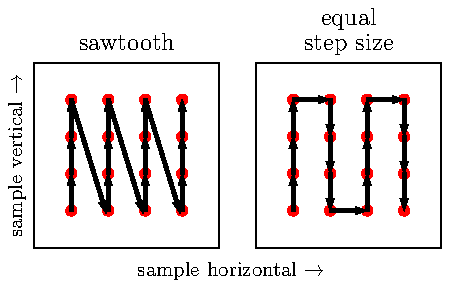
\includegraphics[width=0.75\textwidth]{figures/chap4/rastering_methods.pdf}
	\caption{Schematic of competing raster methods, shown in the sample's reference frame. The clear aperture of the sample is represented by the interior of the black square. The laser propagation direction is out of the page. The laser focal spots are shown as red circles, and the movement of the sample holder relative to the laser focus is indicated by arrows. A 200 $\mu$m border exists between the raster array and the perimeter of the sample's clear aperture. This diagram is to scale for a $1\times1$ mm$^2$ clear aperture sample, a 60 $\mu$m diameter IR focal spot and a 200 $\mu$m step size.}
	\label{fig:Rastering_Methods}
	%figure created using \Python Scripts\rastering\raster_diagram.py
\end{figure}

During the experiment, the sample is rastered across the focus to reduce any deleterious effects of long term uninterrupted laser exposure. During motor movement, the IR beam is blocked with a shutter but the relatively weak XUV beam is allowed to remain on the sample. Each pair of measurements (ground state, excited state) in a delay scan has a unique position on the sample. Typical step sizes are 200 $\mu$m, which is larger than the measured XUV spot size of $\simeq 12 \ \mu \textrm{m}$ and the IR spot size of $\simeq 34 \ \mu \textrm{m}$. Two raster schemes are schematically shown in \cref{fig:Rastering_Methods}. The method shown in the left panel produces a sawtooth pattern on the sample. This method gives very accurate positioning, as the vertical motor is almost always approaching the final position from the same direction. However, the diagonal steps are $\sqrt{N^2 + 1}$ times longer than the vertical steps, where $N$ is the number of vertical steps in the pattern. As a result, there is a bimodal distribution of motor transit times between measurements. If the sample is not fully relaxed between motor movements, this will lead to an inconsistent measurement of the ground state $S_{\textrm{g.s.}}(E)$. Additionally, if the sample is heated by the laser outside of the raster step size, then the average distance between points can affect the measurement of the ground state. The method shown in the right panel alleviates both problems by requiring equal step sizes. Measurements presented in this work were acquired using the method shown in the right panel.

This rastering method has its limitations, as thousands of laser shots hit the sample between each movement. A future upgrade to the beamline could include a rapidly spinning sample mount, as described in \cite{jagerAttosecondTransientAbsorption2018}. Another option would be to directly cool the sample with an \textit{in vacuo} pulsed gas jet pointed at the interaction region, timed such that the valve fires between laser shots.\footnote{Private communication with Prof. Stephen Leone of University of California, Berkeley.}

Before measuring a sample's response for the first time, or after a major optical alignment, an XUV transmission map of the sample must be created. Creating this map serves two purposes: it verifies sample XUV absorption uniformity and it determines the motor coordinates of the sample's clear aperture. To avoid edge effects, the edges of the raster area are chosen to be 200 $\mu$m away from the edge of the clear aperture (see \cref{fig:Rastering_Methods}).

The transient data collection sequence can be summarized as \textit{excited state} $\rightarrow$ \textit{ground state} $\rightarrow$ \textit{move motors}. Details of this sequence are as follows. First, the sample moves to a given raster position and delay wedge position, the IR shutter opens and an excited state spectrum $S_{\textrm{sig}}(\tau, E)$ is recorded. To minimize the duration of the experiment, an XUV reference spectrum $S_{\textrm{vac.}}$ is not recorded. Finally, the sample moves to the next raster position as the delay wedge pair moves to the next delay position. The system is programmed to wait for the wedges to become stationary before the next measurement begins.

Note that in this sequence, the time between the i\textsuperscript{th} excited state and the i\textsuperscript{th} ground state measurement is equal to the exposure time, but the time between the i\textsuperscript{th} ground state measurement and the i+1\textsuperscript{th} excited state measurement is equal to the motor transit time. This sequence is preferable to the alternative (\textit{ground state} $\rightarrow$ \textit{excited state} $\rightarrow$ \textit{move motors}), which would result in a delay step size-dependent relaxation time between the i\textsuperscript{th} excited state and the i+1\textsuperscript{th} ground state measurement.

To further improve our signal-to-noise ratio, we average multiple delay scans together. A typical $\Delta A$ measurement will be repeated between 5 and 50 times. Each delay scan uses the raster points of the previous delay scan so there is a one-to-one mapping of delay to sample position.


\subsection{The Supporting Nitride Membrane}

While most materials have an absorption edge within the range 25 - 150 eV, there are very few commercially available pre-fabricated materials with both the requistite large clear aperture and thickness. Note that either characteristic is relatively easy to achieve individually, but their combination presents unique materials challenges. We considered three synthesis methods to produce this quasi-2D sample:
\begin{enumerate}
	\item sample growth on a traditional substrate, followed by chemical back-etching or milling of the substrate until sub-micron thickness of the heterostructure is achieved;
	\item sample growth on a traditional substrate, followed by mechanical transfer onto a membrane;
	\item sample growth on a membrane.
\end{enumerate}
Sample quality and composition is heavily impacted by local growth conditions such as substrate temperature, deposition rate, substrate crystal cut, substrate-sample lattice mismatch, etc. Many of these characteristics are changed when growing on a substrate of a different cut, or by replacing a substrate with a membrane. In general, one should not expect success when applying a substrate-optimized growth recipe to a freestanding membrane. Therefore, methods 1 and 2 will yield the highest quality samples, as they leverage already-developed sample recipes. However, both methods require a technically difficult second step that is prone to failure.

Selective chemical etching recipes exist for certain compounds, but they usually require an additional chemically intert layer in the heterostructure to protect the sample. Adding this layer will come at the expense of the total XUV flux transmitted by the heterostructure. Additionally, the chemical etching rates are highly dependent on local chemistry, fluid convection and temperature \cite{chiuPhotoluminescenceEvolutionGaAs2015}, which ultimately means that the amount of material removed is uncontrollable and unrepeatable within our requirements (499.9 $\mu$m $\pm$ 10 nm removed from a 500 $\mu$m substrate). For these reasons, we decided to not pursue a chemical etch recipe. Ion or electron milling is more controllable, but too expensive to implement on a large scale. The above reasons preclude the use of Method 1.

Mechanical transfer of thin samples is a tried and true method, but it usually results in flakes with lateral dimensions on the order of 100 $\mu$m. Repeated transfer of many flakes is possible, but there little control over their exact positioning on the membrane. This results in a random distribution of flakes with the possibility of folded or overlapping flakes. These mishaps increase the effective optical density of the sample, changing the IR and XUV absorption properties significantly.

An XUV spatial measurement needs to be taken prior to any ATAS experiment, but a non-uniform distribution of flakes on a membrane would require a much higher resolution map. This is because the flakes are on the order of the XUV and IR focii, so it is critical that the raster points in \cref{fig:Rastering_Methods} correspond to the center of each flake to avoid edge diffraction and to minimize the effects of slow laser pointing drift. For a uniform film, a map can be taken using 200-250 $\mu$m step sizes, as the most important feature is the border of the clear aperture. On the other hand, each flake would have to be sampled $\sim$5 times in each direction to find its center. As a conservative estimate, a membrane covered with $100 \times 100\text{ }\mu$m$^2$ flakes would require a step size of 20 $\mu$m, which increases the number of raster points by a factor of $10^2 = 100$. Considering that a $3 \times 3 \text{ mm}^2$ clear aperture sampled with 200 $\mu$m steps takes $\sim$45 minutes to map, a random distribution of flakes would take a prohibitively long time to map out.

With the first two methods ruled out, we turn to the third method of growing directly on a freestanding membrane. Although it will result in a lower quality sample, it does not have the same technical hurdles of the previous two methods. However, the large clear area makes the heterostructure extremely fragile. We initially attempted to circumvent this problem by using an array of smaller clear apertures.

As shown in \cref{fig:Rastering_Methods}, most of the sample's area isn't directly used by the laser - it exists as a buffer between the grid of sample points. An alternative to a single clear aperture is an array of micro-apertures, each with a diameter on the order of the IR spot size. The micro-apertures exist within a mechanically robust substrate and a thin membrane lies on top of the structure. This configuration significantly eases the material strength requirements by reducing the size of the unsupported area from cm-scale to sub-mm-scale. The regular grid of apertures avoids the difficulties of a randomly distributed sample, easing the XUV mapping step size requirements. Fortunately, these arrays are commercially available from Silson, Norcada (silicon nitride membranes) and US Applied Diamond (diamond membranes) but we encountered technical difficulties in their implementation. Because the aperture size is on the order of the size of the IR focal spot, there is very little room for positioning error, and our motors were insufficiently precise for this application. Further, these arrays are typically only available in at most a $3\times3$ array, which provides an insufficient number of raster points for an ATAS experiment.

\begin{figure}
	\centering
	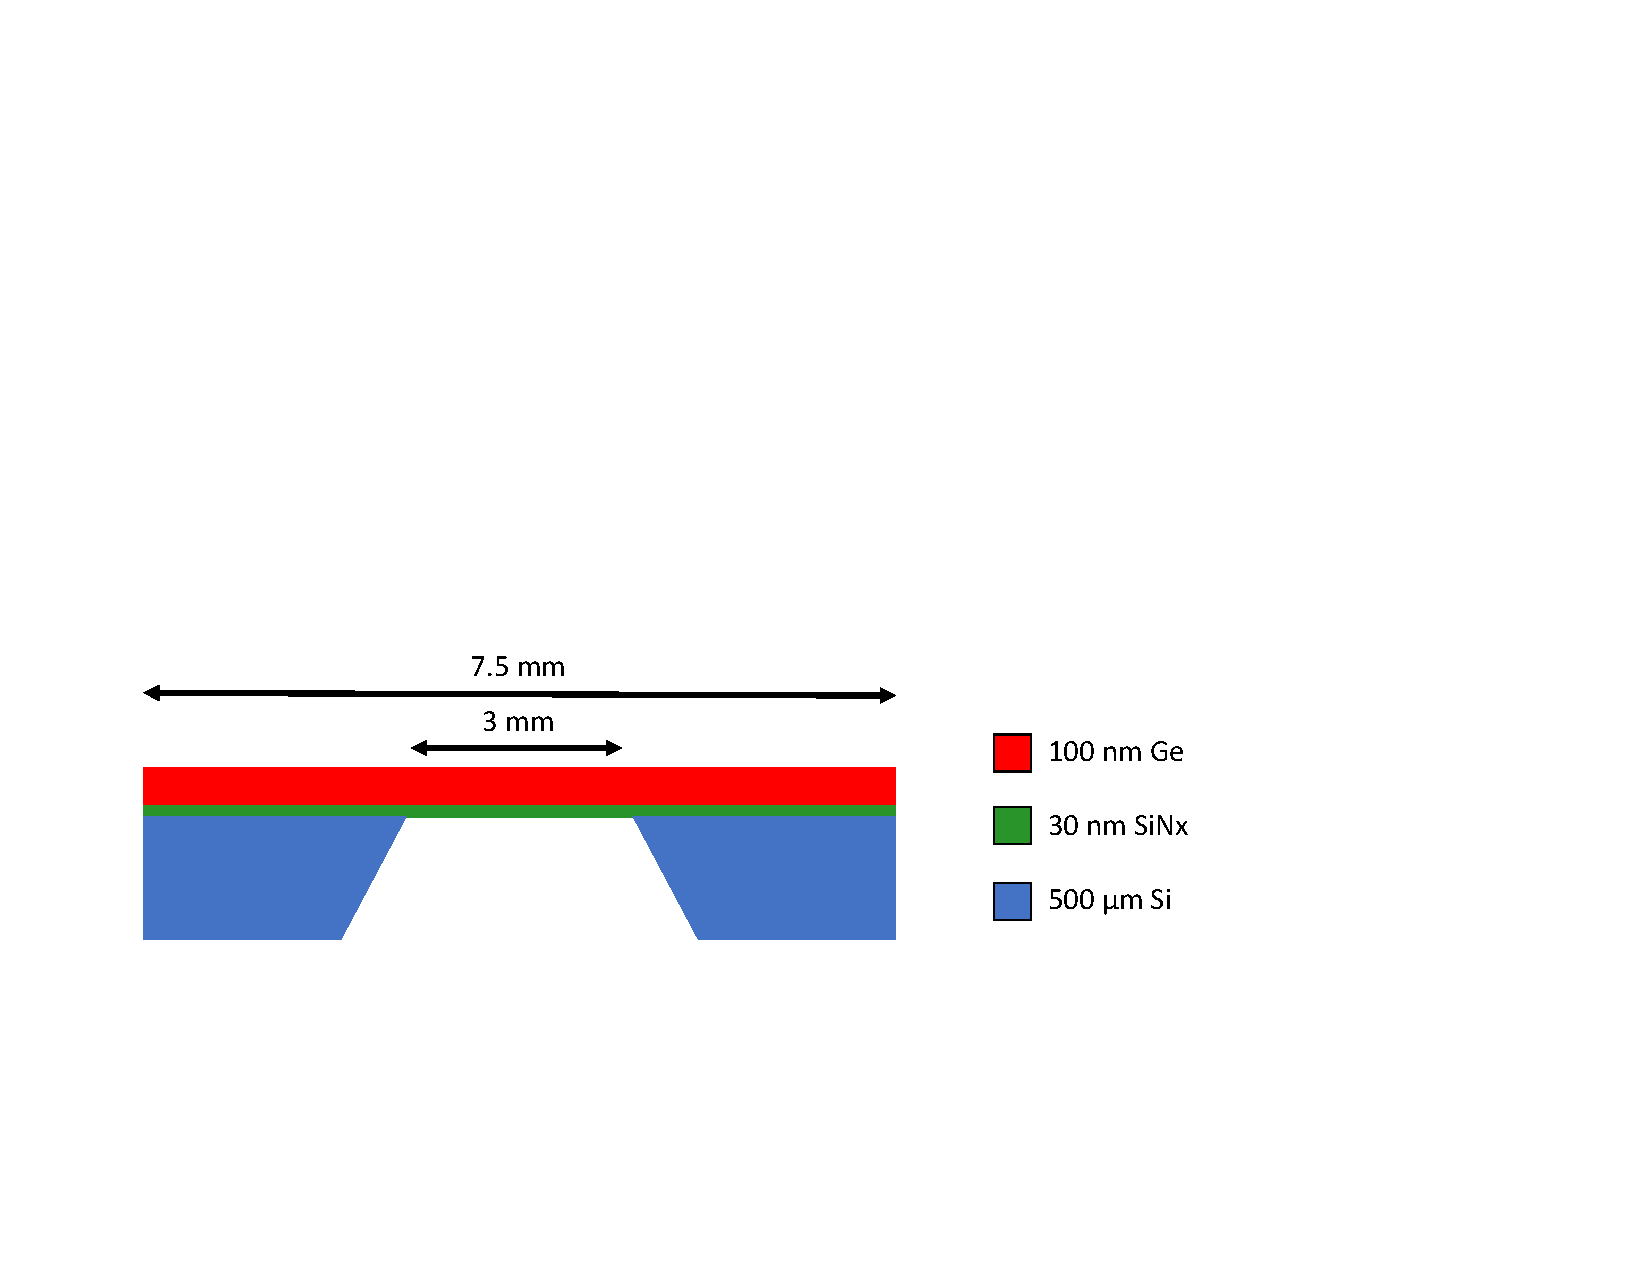
\includegraphics[width=0.75\textwidth]{figures/chap4/Sample_Geometry.pdf}
	\caption{Cartoon showing the cross section of the free standing sample heterostructure. A 500 $\mu$m thick Si frame supports a freestanding 30 nm low stress silicon nitride membrane (Norcada QX7300X), upon which 100 nm of germanium has been deposited. The Si frame has a 3x3 mm$^2$ square clear aperture and a 7.5x7.5 mm$^2$ square external dimension. The taper of the Si frame thickness along the perimeter of the clear aperture forms a knife edge. In an ATAS experiment, the XUV and IR pulses propagate from the top to bottom of the figure.}
	\label{fig:Sample_Geometry}
\end{figure}

With these limitations in mind, we decided to use large aperture x-ray windows from Norcada. These windows consist of a mechanically robust Si frame substrate with a square clear aperture cut through the center. The structure is fabricated so that a thin membrane covers the clear aperture. A schematic of the cross section is shown in \cref{fig:Sample_Geometry}.

\begin{figure}
	\centering
	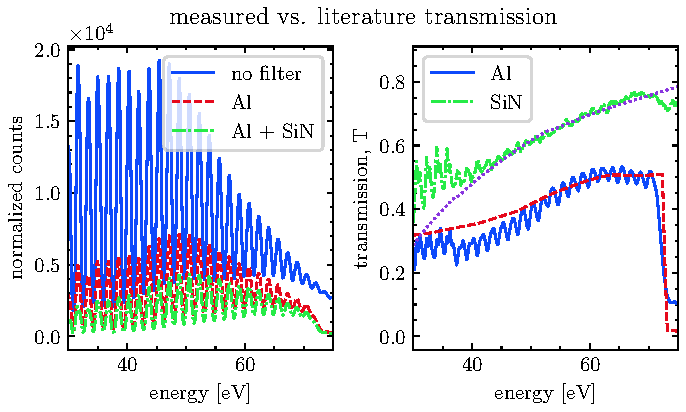
\includegraphics[width=0.75\textwidth]{figures/chap4/SiN_Al_transmission.pdf}
	\caption{XUV transmission measurements of Al metallic filter and silicon nitride membrane. Left panel: normalized XUV counts for i) unfiltered HHG signal, ii) HHG going through a 200 nm Al filter and iii) HHG going through a 200 nm Al filter and 30 nm of silicon nitride. Counts are scaled by the Jacobian. Right panel: transmission curves obtained from the left panel's data. Also shown are literature values for 20 nm of silicon nitride and 200 nm of Al with two 4 nm oxide layers \cite{gulliksonCXROXRayInteractions}. Multilayer interference is not taken into account. Oscillations in measured transmission are numerical artifacts originating from a finite detector noise floor and XUV brightness instabilities.}
	\label{fig:SiN_Al_transmission}
	% dataset: \2019_05_02\
	% plotted using: \Python Scripts\Spectrometer\test\nitride_trans.py
\end{figure}

Norcada offers these structures with either a silicon (polycrystalline or single-crystal) or a silicon nitride membrane. An ideal membrane is transparent to both XUV and IR wavelengths with a high damage threshold. Referring to \cref{fig:Sample_trans_CXRO}, 100 nm of Si provides a relatively flat transmission curve from 25 to 100 eV. In constrast, 30 nm of silicon nitride has poor, but featureless, transmission at lower energies. Both materials transmit light below their bandgaps (5 eV for SiN and 1.14 eV for Si). Finally, silicon nitride's higher bandgap results in a significantly higher laser damage threshold \cite{gamalyAblationSolidsFemtosecond2002,austinFemtosecondLaserDamage2018,keldyshIonizationFieldStrong1965}. Taking all these factors into account, we decided to use 30 nm silicon nitride membranes for germanium transient absorption experiments. The measured transmission of a typical membrane is shown in \cref{fig:SiN_Al_transmission}.

\begin{figure}
	\centering
	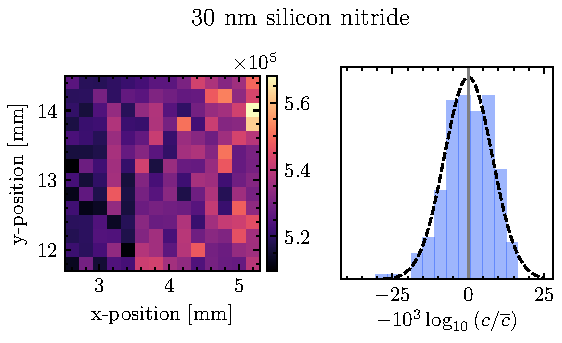
\includegraphics[width=0.75\textwidth]{figures/chap4/nitride_map.pdf}
	\caption{XUV transmission map of 30 nm silicone nitride freestanding membrane. Left panel: integrated XUV counts in the range 30 -- 34 eV. Sample holder motor positions are indicated by x- and y-positions. Right panel: histrogram of logarithmic deviation of counts from the average. Dashed line shows a normal distribution.}
	\label{fig:nitride_map}
	% figure created using \Python Scripts\Spectrometer\test\rastermap.py
	% dataset: C:\testdata\2019_09_10\4_55_32 PM_nitride_map1
\end{figure}

The commercial membranes have very uniform transmission, as shown in \cref{fig:nitride_map}.

\subsection{Laser Damage}
\label{sec:laser_damage}

\begin{figure}
	\centering
	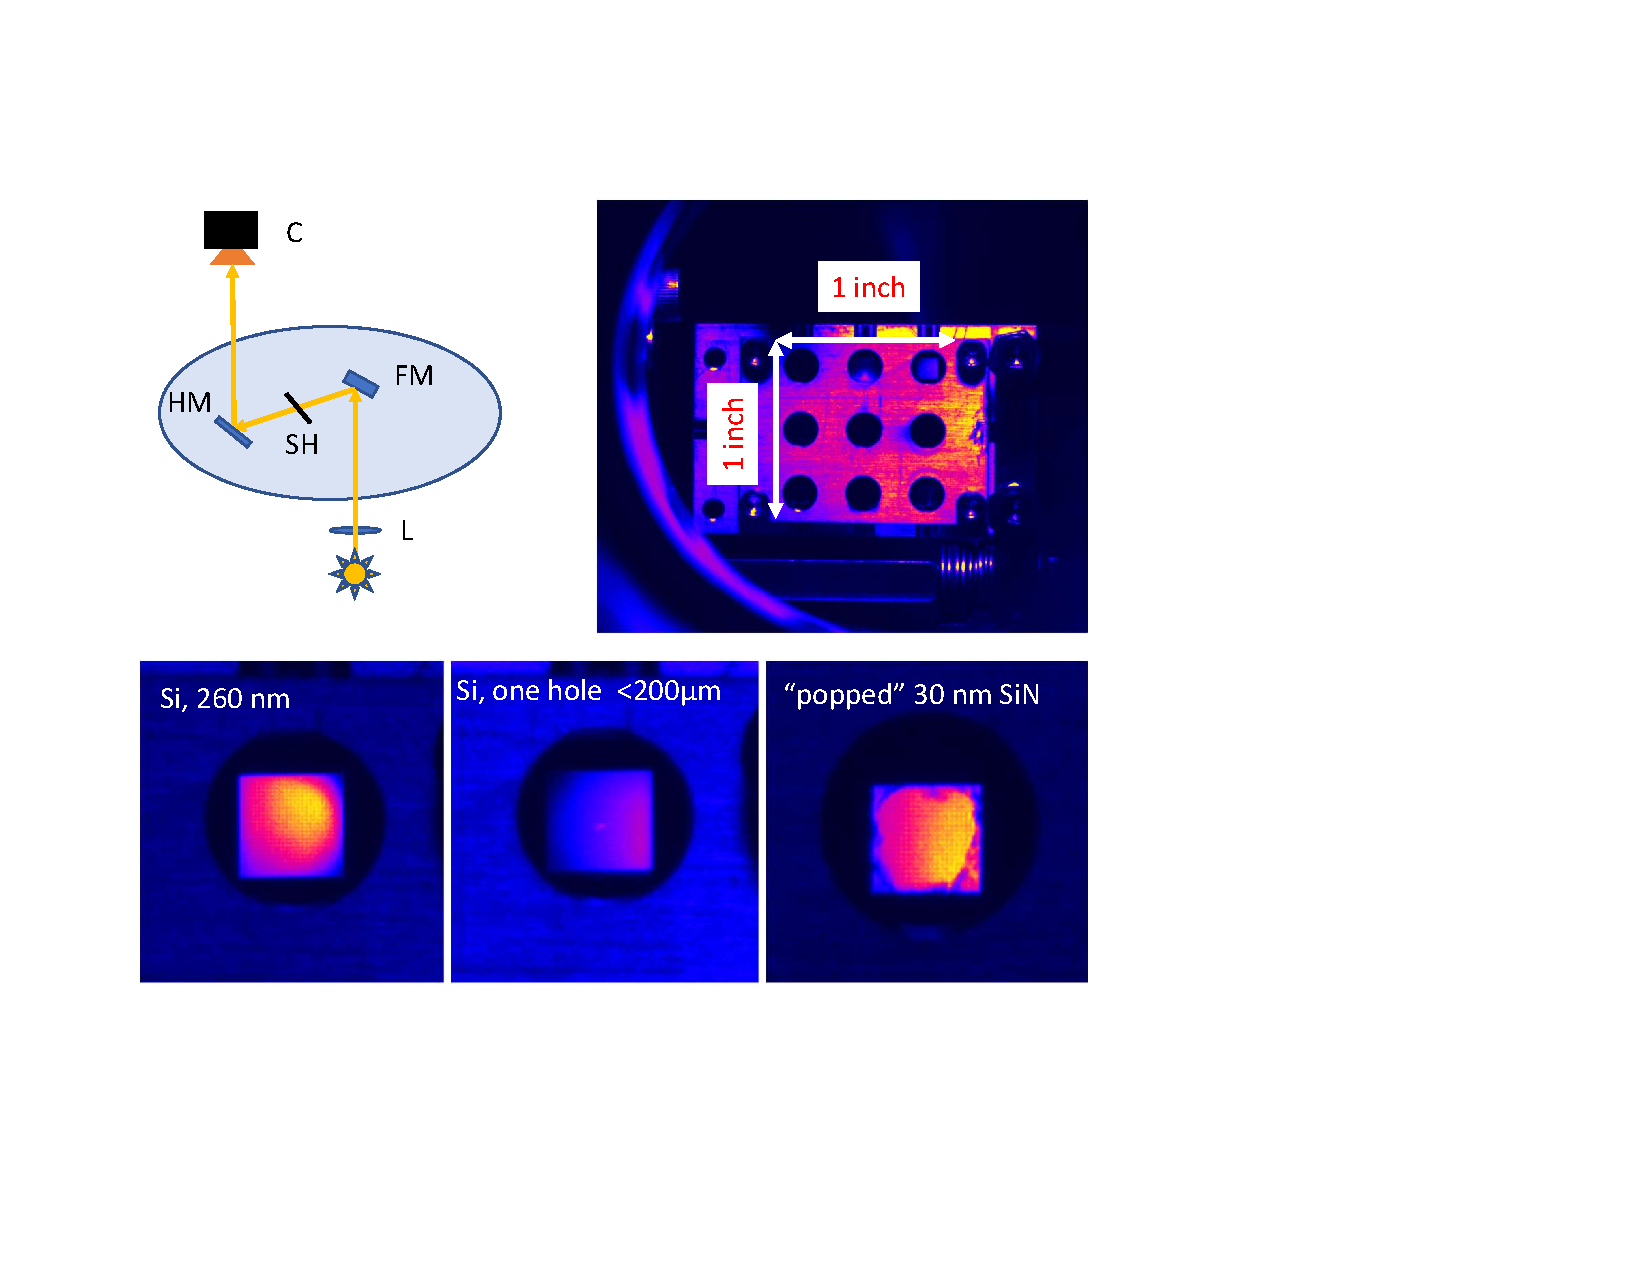
\includegraphics[width=0.75\textwidth]{figures/chap4/sample_holder_damage.pdf}
	\caption{\textit{In-situ} imaging of the samples within the target chamber. Left: optical setup for \textit{in-situ} imaging of samples. C: Si CCD camera, HM: hole mirror, SH: sample holder, FM: translatable silver mirror, L: lens. Right: false color image showing the sample holder with a 3 x 3 grid of 5 mm diameter clear apertures. Samples are held in a clamshell design centered in the clear apertures and are backlit using a flashlight.}
	\label{fig:sample_holder_damage}
\end{figure}

\begin{figure}
	\centering
	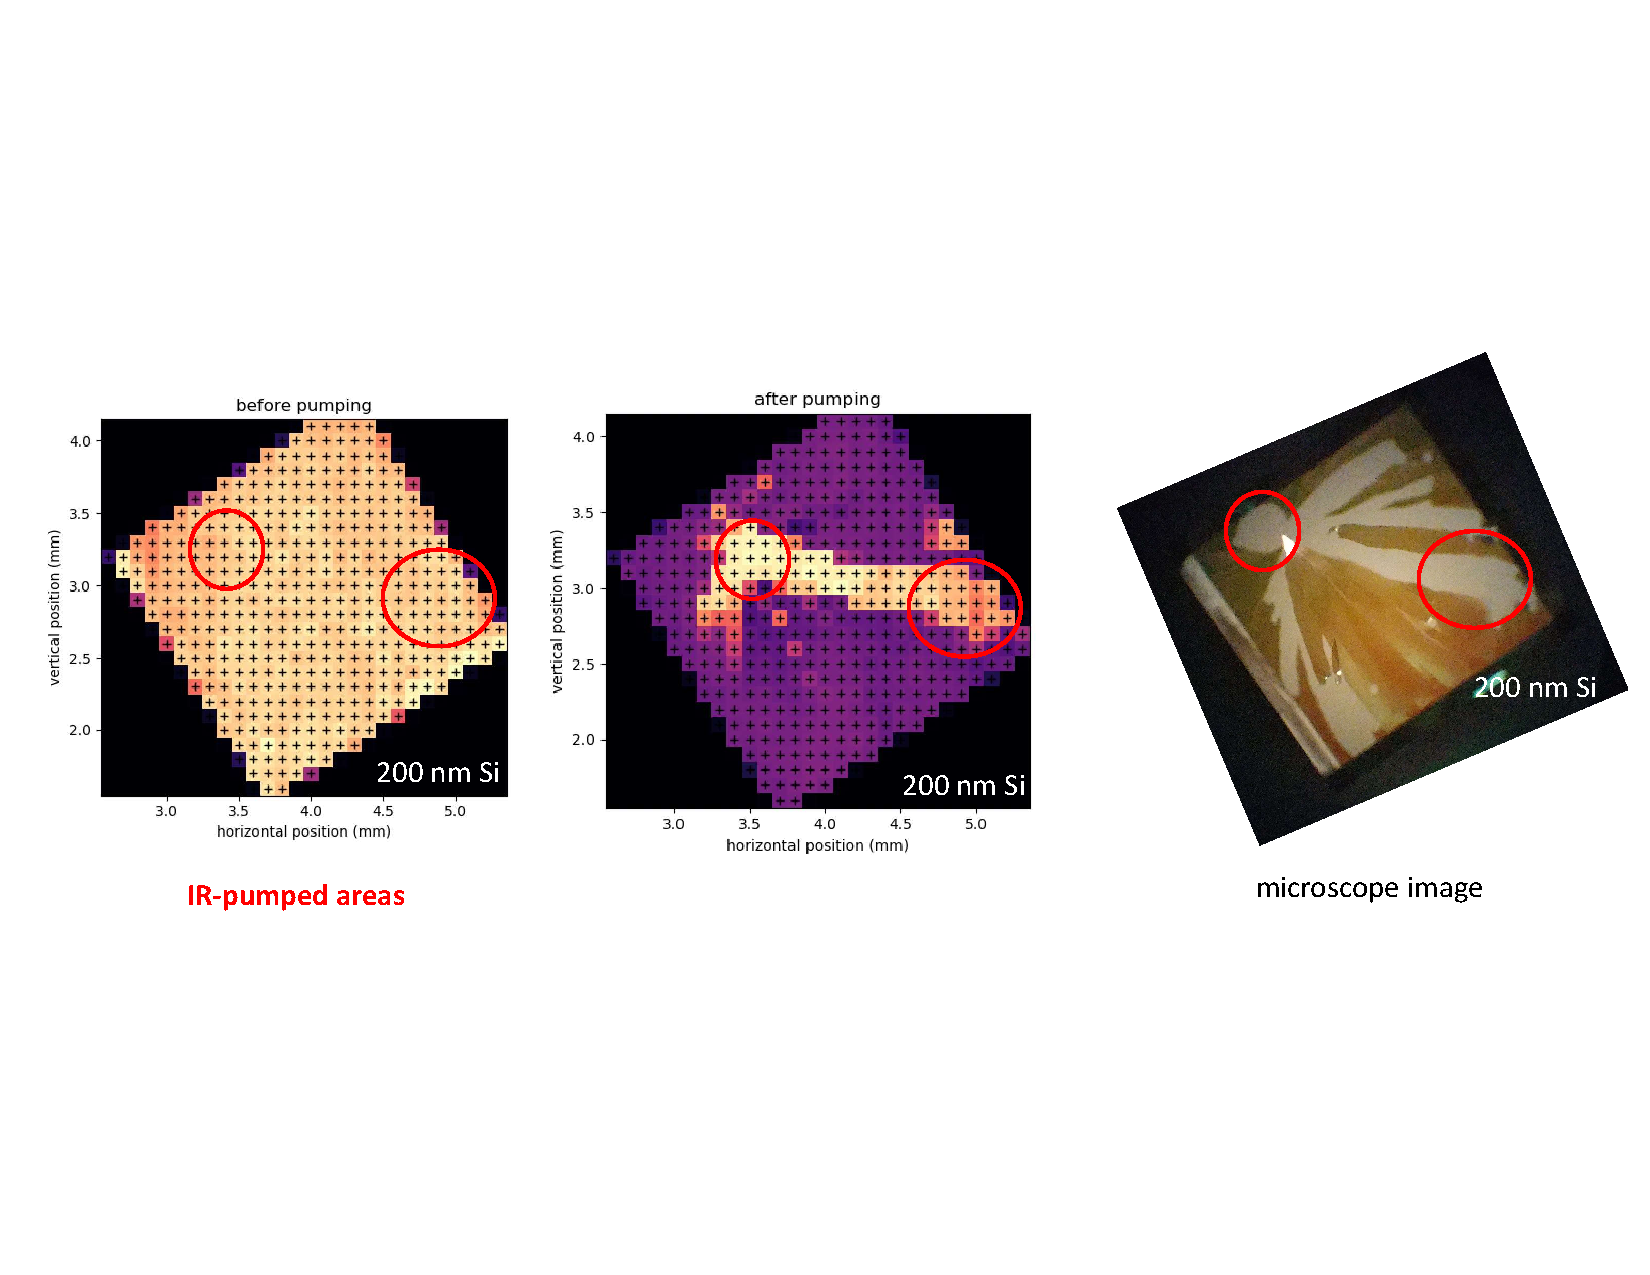
\includegraphics[width=0.9\textwidth]{figures/chap4/Si_damage.pdf}
	\caption{Laser damaged 200 nm silicon membrane samples. Left panel: XUV map of pristine Si before being exposed to IR laser. Center panel: XUV map of damaged sample after being pumped with $\approx \text{ 65 }\mu$J of $\lambda = 1500 \text{ nm}$ at 1 kHz rep. rate in two locations. Right panel: microscope image of damaged sample (beige) showing large sections of missing material (white). Red circles in all three pictures indicate the two locations that were exposed to IR laser light.}
	\label{fig:Si_damage}
\end{figure}

Unlike the gas samples traditionally used in the DiMauro lab, condensed matter samples can suffer permanently laser-induced damage which frustrates any intensity-dependent investigation. The delicate nature of a $\simeq 100 \ \textrm{nm}$ freestanding membrane further complicates these studies. The exact damage mechanism was not studied but we have observed two modes of membrane failure, which will be discussed presently. Occasionally, the volume near the IR focal spot will be ablated by the laser, leaving the rest of the freestanding sample undamaged. The most common failure mode results in the immediate destruction of the entire membrane, often within a single camera exposure ($\simeq 1$ second).

Sample damage is apparent in both the visible and the XUV. The top left panel of \cref{fig:sample_holder_damage} shows our \textit{in-situ} method of imaging the samples using visible light. The top right panel shows a false color image of our sample holder within the chamber. The $3 \times 3$ grid of 5 mm diamter clear apertures is visible as dark circles. The bottom three panels of \cref{fig:sample_holder_damage} show close ups of three samples. On the left, we have a pristine Si membrane; in the middle panel, we have a Si membrane with a $< 200 \ \mu \textrm{m}$ laser-drilled pinhole (visible as a bright point in the center of the membrane); the right panel shows a completely obliterated SiN membrane (visible as ragged edges).

\cref{fig:Si_damage} shows a 200 nm thick freestanding Si membrane before and after it was laser damaged. The first two panels show the integrated XUV transmission ($E \simeq 60-100 \ \textrm{eV}$) as the sample is rastered across the XUV focus; each image consists of over 100 individual measurements. The small black ``+'' signs correspond to the center of the coordinates for each exposure, and the sample is rotated $\simeq 30$ degrees relative to the motor axes. In the left panel, we see the XUV transmission  of a pristine sample before it was exposed to the IR laser. The center panel shows the same sample shortly after it was briefly pumped with $\simeq 65 \ \mu \textrm{J}$ of $\lambda=1500 \ \textrm{nm}$ light at 1 kHz in the two locations indicated by red circles. Damage occured within the first camera exposure (2 seconds). We see high transmission (beige) in a horizontal stripe across the membrane; the remaining parts of the sample have lower transmission (purple), although there are signs of increased transmission in the bottom-center area of the sample. The right panel shows a microscope image of the sample after it was removed from the chamber. We can see that while the areas exposed to the laser are missing, the entire membrane is shattered and is unusable.

Ultrafast melting has been identified as a possible mechanism for mid-IR laser induced damage \cite{austinSemiconductorSurfaceModification2017,austinFemtosecondLaserDamage2018}, which can be understood as the following. At the microscopic level, the germanium lattice consists of a multitude of electronic bonds between valence electrons. In the ground state, there exists an energetic balance between the attractive bonding force and an electrostatic repulsion of inner electrons \& nuclei. As the VB electrons are excited to the CB, the attractive force is weakened and the bond distance increases. If we continue to excite the VB, it will become depleted to the point where the repulsive forces destroy the bonds. Thereafter, the material no longer resists shear forces - much like a liquid. Experiments have shown that the lattice is destroyed within 100 fs after the electron-hole plasma is created, and the crystal melts 500 fs later. In semiconductors, tight-binding calculations predict that ultrafast melting occurs when the conduction band density $N_{\textrm{CB}}$ is about 8-12\% of the valence band density $N_{\textrm{VB}}$ \cite{stampfliTheoryLaserinducedInstability1990,austinFemtosecondLaserDamage2018}.

We estimate the valence band electron density of the ground state as the product of the number of valence electrons per atom and the number of atoms per unit cell divided by the unit cell volume. Germanium has a diamond cubic lattice with a unit cell volume of ${a^3 = (5.658 \ \AA)^3 = 1.81129 \times 10^{-22} \ \textrm{cm}^3}$, and an electron configuration of ${[\textrm{Ar}] 3\textrm{d}^{10 }4\textrm{s}^2 4\textrm{p}^2}$. With 8 atoms per unit cell and 4 valence electrons per atom, the valence band electron density of the ground state is $N_{\textrm{VB}} = 1.767 \times 10^{23} \ \textrm{cm}^{-3}$. Therefore, we would not expect ultrafast melting to occur unless $N_{\textrm{CB}}$ exceeds $\simeq 1.767 \times 10^{22} \ \textrm{cm}^{-3}$.

\textbf{slower heating (average power)}

two mechanisms of sample damage (microscopic level): slower heating (average power) vs instaneous damage (peak power)

two ways samples get destroyed (macroscopic level): pinhole drilled vs membrane popped.

%\subsection{Estimation of Excited Carrier Density}
%\label{sec:estimate_excited_carrier_density}
%
%We are concerned with two quantities: the peak excitation fraction in the sample and the average excitation fraction at the location of the XUV focus. The former quantity is relevant when considering sample damage, whereas the latter will be proportional to the measured signal. If the XUV and IR spots are perfectly overlapped at the sample plane, then these two quantities are approximately equal. We first calculate the peak excitation fraction, then we consider how a misaligned beam will affect the measured signal.
%
%The laser propagation calculations in \cref{fig:pump_on_focus_calculation} were done for vacuum, but we are concerned with the field in our sample. The electric field inside a dielectric $E_{\text{int}}$ is related to the external electric field by the following equation \cite{schultzeAttosecondBandgapDynamics2014}:
%\begin{equation}
%E_{\text{int}} = \frac{2}{1+\sqrt{\epsilon}} E_{\text{ext}}
%\label{eqn:internal_external_Efield}
%\end{equation}
%where $E_{\text{int}}$ is the electric field inside the sample, $E_{\text{ext}}$ is the electric field outside the sample, $\epsilon$ is the dielectric constant and its square root is the refractive index $n_{\text{IR}}$. The internal intensity $I_{\text{int}}$ is the square of the internal electric field. For germanium at $\lambda$ = 1430 nm, $n_{\text{IR}}$ = 4.2481, and we have the following relations:
%\begin{equation}
%\begin{aligned}
%E_{\text{int}} &= 0.381 \times E_{\text{ext}} \\
%I_{\text{int}} &= 0.145 \times I_{\text{ext}}
%\end{aligned}
%\end{equation}
%
%Given our laser paremeters, we can estimate the highest carrier density within the sample. First, we estimate the absorbed laser fluence, $F_{\text{abs}}$ \cite{harbCarrierRelaxationLattice2006}:
%\begin{equation}
%F_{\text{abs}} = F_{\text{inc}} \left(1-R\right) \left( 1-\exp(-\alpha L) \right) \left(1+R \exp(-\alpha L)\right),
%\label{eqn:absorbed_fluence}
%\end{equation}
%where $F_{\text{inc}}$ is the incident fluence, $R$ is the reflectivity equal to the square of the Fresnel coefficient, $\alpha$ is the absorption coefficient and $L$ is the sample thickness. The bracketed terms in \cref{eqn:absorbed_fluence} are the fraction of fluence transmitted by the first surface, the fraction absorbed by a single pass through the sample, and the additional absorption due to a back reflection off the rear face of the sample. Note that the back-propagating beam will arrive (on average) at a delay of $n_{\text{IR}} L/(2c) \approx 0.7 \text{ fs}$ later than the forward-propagating beam. This time scale is nearly two order of magnitude less than the IR pulse duration, so we should expect any electron dynamics initiated by the back reflection to contribute to the measured signal.
%
%If each absorbed photon corresponds to an excited electron, then the excited carrier density $\Delta N$ is given by the following expression \cite{cushingDifferentiatingPhotoexcitedCarrier2019}:
%\begin{equation}
%\Delta N = \frac{F_{\text{abs}}}{\hbar \omega} \frac{1}{L},
%\label{eqn:excitation_fraction}
%\end{equation}
%where $\hbar \omega$ is the IR photon energy. In \cref{eqn:excitation_fraction}, the quantity $F_{\text{abs}} / (\hbar \omega)$ represents the number of absorbed photons per unit area; dividing this quantity by the sample thickness gives the number of absorbed photons per unit volume. This assumes that the skin depth of the material is greater than membrane thickness, which is true for germanium at these wavelengths.
%
%Finally, we convert the excited carrier density to a fractional excitation. Germanium has $N_{\text{u.c.}}=2$ valence electrons per unit cell, and each unit cell has a volume $V_{\text{u.c.}}=4.527 \times 10^{-23} \text{ cm}^{3}$. Therefore the fractional carrier excitation is
%\begin{equation}
%f = \Delta N \frac{V_{\text{u.c.}}}{N_{\text{u.c.}}}
%\end{equation}
%
%We can use literature values for 100 nm of germanium pumped at $\lambda$ = 1430 nm light. From the literature \cite{nunleyOpticalConstantsGermanium2016}, $R = 0.38315$, $\alpha = 5803.4 \text{ cm}^{-1}$, and so $F_{\text{abs}} = 0.0413 \times F_{\text{inc}}$. Therefore, only about 4.13\% of the incident fluence is absorbed by the sample.
%
%According to the calculations in \cref{fig:pump_on_focus_calculation}, for each 1 $\mu$J energy input pulse (measured at L4), 0.413 $\mu$J makes it to the focal plane. 49\% of that energy is within the main lobe, which contains 0.202 $\mu$J of energy. Approximating the central lobe as a Gaussian beam with a FWHM of 35 $\mu$m and a pulse energy of 0.202 $\mu$J, the peak fluence is calculated by dividing the total energy of the Gaussian by $\pi w^2/2$. The Gaussian beam waist $w$ is related to the FWHM via $w^2 = \text{FWHM}^2 / (2 \ln 2)$. Thus, for each 1 $\mu$J input energy, the peak fluence in the central lobe is 14.6 mJ/cm$^2$ and the absorbed peak fluence is 0.60 mJ/cm$^2$. This corresponds to an peak excited carrier density of $4.3 \times 10^{20} \text{ cm}^{-3}$ and an excitation fraction of 0.98\% (per 1 $\mu$J of input energy).

\section{Finite Beam Size Considerations: Measuring $\Delta A$}
In a transient absorption experiment, we measure the change in absorbance of the sample in response to a laser-induced electronic excitation. We measure macroscopic properties in the lab, but the coefficients are determined by the local conditions at the microscopic level. In this section, we will describe how the two quantities are related given the XUV and excited fraction spatial profiles. We will use this formalism to calculate the sensitivity of our measurement to the relative spot sizes of the IR excitation laser and the XUV probe beam. Additionally, we will calculate the sensitivity of the measurement to misalignment of the two focal spots.

\subsection{Relating Macroscopic and Microscopic Absorbance}
\label{sec:micro_macro_DeltaA}

The XUV absorption within the sample is linear, so we can write the measured spectrum $S_i$ as the product of the input XUV brightness $I_{\textrm{XUV}}$ and a transmission factor $T_i$:
\begin{equation}
\begin{aligned}
S_i(E, \tau) &= I_{\textrm{XUV}}(E) \ T_i(E, \tau), \\
\textrm{with} \ T_i &= 10^{- A_i}, \\
\textrm{and} \ A_i &= \int_{0}^{L} \alpha_{10}(E, z) \dd{z},
\end{aligned}
\label{eqn:DeltaA_macro}
\end{equation}
where $A_i$ is the absorbance and $S_i(E,\tau)$ is the recorded XUV spectrum with photon energy $E$ at XUV-IR delay $\tau$. The subscript $i$ denotes a ground state (g.s.) or excited state (e.s.) measurement. Note that \cref{eqn:DeltaA_macro} assumes no transverse spatial structure of the ionization fraction or the XUV light, so $S_i, \ I_{\textrm{XIV}}, \ T_i, \ A_i$ and $\alpha_{10}(z)$ are effectively macroscopic quantities. In our experiments, we measure the area integral of the spectrum in the far-field:
\begin{equation}
S_{\textrm{meas},i} = \iint \dd{x} \dd{y} I_{\textrm{XUV}}(x,y) \ t_i(x,y),
\end{equation}
where $t_i(x,y)$ is the \textit{local transmission} of the sample/heterostructure at sample position $(x,y)$.\footnote{In the following discussion, we drop the explicit energy- and time-dependence to make the equations more readable. The time dependence comes from the evolution of the ionization fraction $\eta$, and the energy dependence comes from the energy-dependent excitation and ground state of the sample. Also note that the XUV beam shape does not appreciably change over the sample thickness (since $z_R \simeq 1 \ \textrm{mm} \gg 100 \ \textrm{nm}$), so we omit the $z$-dependence in writing $I_{\textrm{XUV}}(x,y)$.}  Therefore, the (macroscopic) transmission and absorbance of the excited or ground state relative to a vacuum reference can be expressed as:
\begin{equation}
\begin{aligned}
T_i &= \frac{S_i}{S_{\textrm{vac.}}} = \frac{\iint \dd{x} \dd{y} I_{\textrm{XUV}}(x,y) \ t_i(x,y)}{ \iint \dd{x} \dd{y} I_{\textrm{XUV}}(x,y)} \\
A_i &= - \log_{10}(T_i)
\end{aligned}
\end{equation}
Using this notation, the \textit{change in absorbance} between the excited and ground states is:
\begin{equation}
\Delta A \equiv A_{\textrm{e.s.}} - A_{\textrm{g.s.}} = - \log_{10} \left( \frac{\iint \dd{x} \dd{y} I_{\textrm{XUV}}(x,y) \ t_{\textrm{e.s.}}(x,y)}{\iint \dd{x} \dd{y} I_{\textrm{XUV}}(x,y) \ t_{\textrm{g.s.}}(x,y)} \right)
\label{eqn:Delta_A_2}
\end{equation}
Now, let us write the cross section $\alpha$ of the sample as a ground state term plus an ionization-dependant perturbation term:
\begin{equation}
\begin{aligned}
\alpha(x,y,z) &= \alpha_{10} (1 + \eta(x,y,z)) \\
\textrm{with} \quad \alpha_{10} &\equiv \frac{\alpha_e}{\ln 10} = \frac{4 \pi \Im [\tilde{n}]}{\lambda \ln 10}.
\end{aligned}
\end{equation}
From \cref{eqn:DeltaA_macro}, the absorbance of a sample of thickness $L$ is:
\begin{equation}
\begin{aligned}
A_{\textrm{g.s.}} &= \alpha_{10} L, \\
A_{\textrm{e.s.}} &= (\alpha_{10} + \bar{\eta}_z(x,y)) L.
\end{aligned}
\end{equation}
where we have defined the \textit{depth-averaged excitation fraction}, $\bar{\eta}_z(x,y)$ as:
\begin{equation}
\bar{\eta}_z(x,y) \equiv \frac{1}{L} \int_{0}^{L} \eta(x,y,z) \dd{z}.
\label{eqn:eta_z}
\end{equation}
Since $t_{\textrm{g.s.}}(x,y)$ is spatially invariant, \cref{eqn:Delta_A_2} simplifies to:
\begin{equation}
\Delta A = -\log_{10} \left( \frac{ \iint \dd{x} \dd{y} I_{\textrm{XUV}}(x,y) 10^{- \alpha_{10} L \bar{\eta}_z(x,y)}}{ \iint \dd{x} \dd{y} I_{\textrm{XUV}}(x,y)} \right).
\label{eqn:Delta_A_3}
\end{equation}
Therefore, the measured macroscopic sample response is the integral of the local absorbance weighted by the local XUV probe intensity. \cref{eqn:Delta_A_3} will reduce to the \cref{eqn:DeltaA_macro} if and only if $\bar{\eta}_z(x,y)$ is constant for all values of $x$ and $y$. Since $\bar{\eta}_z(x,y)$ is created in response to the IR laser, this is equivalent to making the plane wave approximation for the pump arm. In the case of finite excitation and probe beams, the measured macroscopic response of the sample will always be lower than that predicted by the \textit{peak excitation fraction}, $\textrm{Max}[\eta(x,y,z)]$. 

Our condensed matter experiments are limited by our ability to measure weak signals. We can improve the measured signal by increasing the depth-averaged excitation fraction, but we are constrained by the ultrafast melting condition ($N_{\textrm{CB}} \simeq 0.1 N_{\textrm{VB}}$), which puts an upper limit on the peak excitation fraction $\textrm{Max}[\eta(x,y,z)]$. Our detection efficiency, defined as the measured $\Delta A$ divided by $\Delta A$ at the peak excitation fraction, is an important experiment parameter. In the following disussion, we consider the effect of the transverse profile on the measurement efficiency. In \cref{sec:thin_film_interference} we will see that the thin film interference causes a strong $z$-dependence of $\eta(x,y,z)$ that will further diminish the measurement efficiency.

We can gain intuition about the situation by numerically evaluating \cref{eqn:Delta_A_3} using mathematically convenient expressions for $I_{\textrm{XUV}}$ and $\bar{\eta}_z$:
\begin{equation}
\begin{aligned}
I_{\textrm{XUV}} (x,y,z) &= \frac{2}{\pi w(z)^2} \exp \left( - \frac{2 (x^2 + y^2)}{w(z)^2} \right), \\
\bar{\eta}_z(x,y) &= \eta_0 \exp \left( -\frac{2(x^2 + y^2)}{w_1^2} \right), \\
\textrm{with} \ w(z) &= w_0 \sqrt{1 + (z/z_R)^2}, \\
\textrm{and} \ w_1 &\equiv a*w_0.
\end{aligned}
\label{eqn:XUV_eta_expressions}
\end{equation}
In the above, we have made the radius of the depth-averaged excited fraction $a$ times larger than the XUV spot radius. Additionally, the XUV intensity is normalized such that the denominator in \cref{eqn:Delta_A_3} evaluates to $1$. In \cref{fig:Delta_A_curve}, we numerically integrate \cref{eqn:Delta_A_3} using the assumptions of \cref{eqn:XUV_eta_expressions} to better understand the importance of the relative sizes the XUV and depth-averaged ionization fraction spot sizes. The left panel shows the efficiency of measuring the amplitude $\eta_0$ for a given ratio of spot sizes. We see an error function-like curve which approaches unity as $a \rightarrow \infty$, which is consistent with the plane wave approximation. Equal spot sizes result in a measured $\Delta A$ that is only 40.7\% of the amplitude $\alpha_{10} L \eta_0$, and an XUV spot size 1/3 of the excited fraction results in an efficiency of 89\%. In our experiment, the XUV beam waist radius is $\simeq 6 \ \mu \textrm{m}$ and the IR FWHM is $\simeq 34 \ \mu \textrm{m}$, which yields $a \simeq 5$ and a detection efficiency of $\simeq 96\%$. In the right panel, we plot the expected measured signal as a function of the effective excitation cross section for different values of $a$.

Note that we obtain $a=5$ using our XUV optic with a demagnification factor of 3. If instead we used a 1-to-1 toroid to focus the XUV onto the sample, we would have $a=5/3$, and the measurement efficiency would be $\simeq 65\%$. Therefore, the ellipsoid's demagnification yields a 50\% increase in signal compared to a 1-to-1 toroid.

\begin{figure}
	\centering
	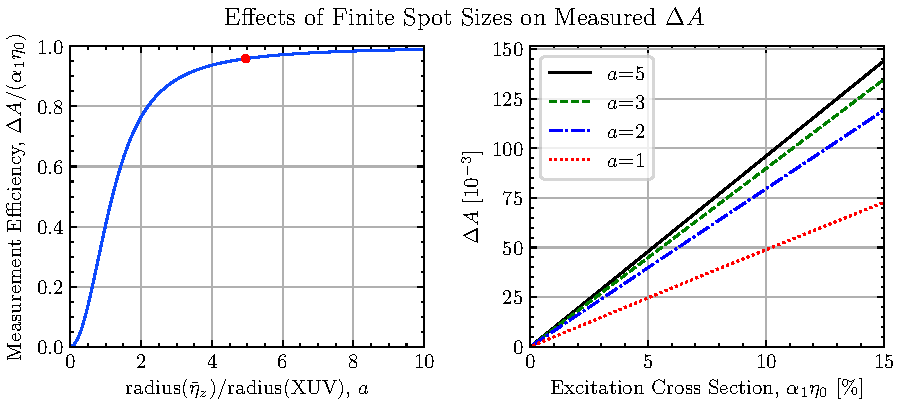
\includegraphics[width=0.9\textwidth]{figures/chap4/Delta_A_curves.pdf}
	\caption{The effect of finite pump and probe sizes in measuring the change in absorbance in an ATAS experiment. Left panel shows the relative sensitivity of $\Delta A$ as a function of the relative sizes of the XUV and $\bar{\eta}_z$ spots. The red dot represents our experimental configuration ($a\simeq 5$), which yields $\simeq 96\%$ measuring efficiency. The right panel shows the expected $\Delta A$ amplitudes as a function of both $a$ and $\alpha_{10} L \eta_0$. See \cref{eqn:Delta_A_3} and surrounding text for details.}
	\label{fig:Delta_A_curve}
	% plot made with \Python Scripts\DrakeIonization\plot_DeltaA_function.py
\end{figure}


\subsection{XUV-IR Misalignment}

\begin{figure}
	\centering
	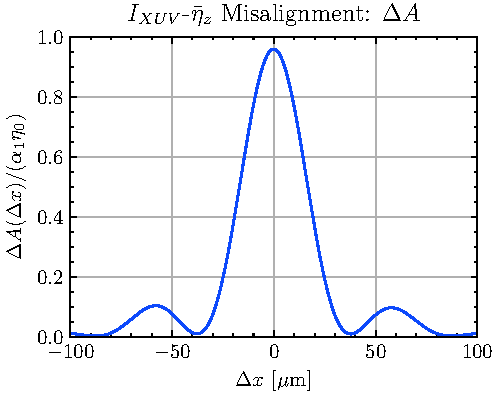
\includegraphics[width=0.75\textwidth]{figures/chap4/XUV_eta_misalignment.pdf}
	\caption{The effect of relative misalignment of the IR and XUV spots. We assume linear excitation of the sample for this calculation.}
	\label{fig:XUV_eta_misalignment}
	% plot made with \Python Scripts\DrakeIonization\VolumeAveraging_class_script.py
\end{figure}

We now consider the effect of having slightly misaligned IR and XUV spots. For this calculation, we assume the sample excitation is purely linear: $\eta(x,y) \propto I_{\textrm{IR}}(x,y)$. We numerically integrate \cref{eqn:Delta_A_2} using the simulated IR intensity profile $I_{\textrm{IR}}(x,y)$ from \cref{fig:pump_on_focus_calculation} and an XUV spot with a 6 $\mu$m waist and a transverse offset of $x \rightarrow x+\Delta x$. The result is shown in \cref{fig:XUV_eta_misalignment}. As in \cref{fig:Delta_A_curve}, we see that the finite beam sizes lead to a maximum measurement effiency of about 96\%. The measurement is very sensitive to misalignment; a 10 $\mu$m offset will reduce the efficiency to 76\%, a 20 $\mu$m deviation yields 37\%, and the minimum of $\simeq 0.8\%$ is near $\Delta x = \pm 37 \ \mu \textrm{m}$. The local maximum at $\Delta x = \pm 58 \ \mu \textrm{m}$ is due to the \nth{1} lobe of the IR diffraction pattern, yielding an efficiency of $\simeq 10\%$.

%We have yet to calculate the sensitivity of spatial overlap to deviations in the input laser pointing.
In our chamber, a 10 $\mu$m displacement of the IR at the sample corresponds to a 15 $\mu$rad tilting of the hole mirror (HM). There are two ways misalignment can affect experimental results. If the relative positions of the XUV and IR focal spots changes as an experiment is performed, then the recorded ATAS signal would be a function of both the laser-induced dynamics and the XUV-IR spatial misalignment. On the other hand, if the entire experiment is performed using a constant misalignment, we would be exciting the sample to some peak excitation fraction $f$, but our probe would be measuring a lower excitation fraction ($\approx f a / a_{max}$). Consequently, the measured ATAS signal would be lower than otherwise expected, and any attempts to boost the signal by increasing the interaction intensity could result in permanent laser-induced sample damage.

A condensed matter ATAS experiment has much tighter alignment tolerances than a gas phase experiment. This discrepancy is a simple consequence of sample geometry and density. In either experiment, the measured signal comes from the region of space where the sample density, XUV intensity and IR intensity overlap. The transmission of XUV through the sample is, to first order, $T= \exp(- n \mu_a L)$, where $n$ is the number density, $L$ is the sample thickness and $\mu_a$ is the photoabsorption cross section. As discussed above, for technical reasons the experiment should be designed with $T \approx 1/2$. Therefore, the product $n \mu_a L$ will be approximately constant for any transient absorption experiment.

The number density of a condensed phase sample is determined by the chemistry of the compound and is on the order of $4 \times 10^{22} \text{ atoms}/\text{cm}^3$. The experimentalist is free to engineer clever sample geometries, heterostructures and/or nanopatterns, but the high atomic density (and thus absorption coefficient) dictates a total sample thickness on the order of 100 nm. On the other hand, the spatial profile and density of a gas phase sample is determined by the gas nozzle design and its backing pressure, respectively. A typical nozzle used in our lab produces a gas plume with lateral dimensions on the order of 200 - 500 $\mu$m. This effectively creates a sample that is three orders of magnitude thicker than a condensed phase sample, which relaxes the alignment constraints significantly. This has important consequences for the alignment of the sample.

If the XUV and IR are perfectly collinear, then the beam overlap region is effectively infinite in the propagation direction. In this case, the measured $\Delta A$ will be finite regardless of any displacement of the sample plane from the focal plane, and maximal when the sample lies in the focal plane. However, if there is a small angle $\delta \theta$ between their $k$-vectors, then the beams will only spatially overlap within a finite region. In this case, the position of the sample plane relative to the beam crossing plane becomes a critical experimental parameter. For an infinitely thick sample (i.e., a chamber effusively filled with gas), it wouldn't matter where the beams crossed as long as they overlapped somewhere within the chamber. Then, the XUV-$\eta$ overlap integral would decrease as a function of $\delta \theta$, but it would never go to zero. For a thin sample, the bounds of \cref{eqn:eta_z} must enclose the beam overlap region, or else the integral will be zero. Thus, the signal strength of a condensed phase ATAS experiment is roughly 3 orders of magnitude more sensitive to the $z$-position of the sample relative to the focal plane than a gas phase ATAS experiment.


\section{Nonlinear Excitation of Germanium}
\label{sec:nonlinear_excitation_germanium}

\begin{table}[]
	\centering
	\begin{tabular}{ll}
		{\ul effective electron masses} &  \\
		$m_{\textrm{CB}}$, for direct transitions & $0.041 * m_e$ \\
		$m_{\textrm{CB}}$, for indirect transitions & $0.0815 * m_e$ \\
		$m_{\textrm{VB}}$, from HH & $0.33 * m_e$ \\
		$m_{\textrm{VB}}$, from LH & $0.043 * m_e$ \\
		$m_{\textrm{VB}}$, from SO & $0.084 * m_e$ \\
		&  \\
		{\ul ground state band gaps} &  \\
		direct transitions, from LH/HH & 0.8 eV \\
		direct transitions,  from SO & 0.828 eV \\
		indirect transitions,  from LH/HH & 0.67 eV \\
		indirect transitions, from SO & 0.668 eV \\
		&  \\
		electron-phonon collision time, $\Gamma^{-1}$ & 47 fs
	\end{tabular}
	\caption{Material parameters used in the Keldysh simulation for germanium. Notation used is as follows: CB = conduction band, VB = valence band, HH = heavy hole band, LH = light hole band, SO = split-off band.}
	\label{tab:Keldysh_parameters}
\end{table}

We estimate the excitation fraction in the sample by performing numerical simulations\footnote{Special thanks to Dr. Drake Austin for performing the simulations, and to Professor Enam Chowdhury for arranging the collaboration and participating in helpful discussions.} of the electronic excitation using the Keldysh formalism \cite{sergaevaUltrafastExcitationConductionband2018,keldyshIonizationFieldStrong1965,vpopruzhenkoKeldyshTheoryStrong2014}. The simulation uses a modified Keldysh model that accounts for different band shapes (parabolic or cosine), valence band depletion, and multiple excitation channels. Germanium has a direct bandgap of $\Delta^{\textrm{dir.}} = 0.8 \ \textrm{eV}$, an indirect bandgap of $\Delta^{\textrm{ind.}} = 0.66 \ \textrm{eV}$, and a split-off band $\Delta_{\textrm{SO}} = 0.29 \ \textrm{eV}$ below the heavy and light hole valence bands. Additional material parameters are listed in \cref{tab:Keldysh_parameters}. Focal volume averaging is performed taking into consideration the diffraction from the hole mirror at the focal plane (see \cref{sec:Pump_Arm_Focus_Calculations,fig:pump_on_focus_calculation}) and thin film interference. In this section, we give a description of the nonlinear model (\cref{sec:nonlinear_excitation_model_details}), a method for handling indirect transitions (\cref{sec:indirect_transitions}), thin film interference calculations (\cref{sec:thin_film_interference}), a discussion about the bandwidth of the pulse (\cref{sec:bandwidth_of_pulse}), and the main results of the simulation (\cref{sec:nonlinear_excitation_results}).

\subsection{Description of the Nonlinear Model}
\label{sec:nonlinear_excitation_model_details}

This model considers photoexcitation from the top of the three valence bands to the first conduction band. In germanium, the gap between the bottom of the first conduction band and vacuum is about 4 eV, so photoemission can be neglected. It includes both direct and indirect transition pathways. We start with the time-dependent electron density per unit energy that is a function of time and electron energy in the conduction band:
\begin{equation}
N(t, \epsilon) = \sum_{i} N_i(t, \epsilon); \quad \dv{N_i(t, \epsilon)}{t} = f_i(t) W_i [F(t)],
\end{equation}
where the subscript $i$ denotes heavy-hole (HH), light-hole (LH) and split-off (SO) valence bands, and $f_i(t)$ are the population coefficients:
\begin{equation}
f_i(t) = 1 - \frac{1}{N_{i0}} \int_{\epsilon_{i0}}^{\infty} N_i(t,\epsilon) \dd{\epsilon}
\end{equation}
determined via the initial total population of each valence band $N_{i0}$ (units of 1/cm\textsuperscript{3}). The initial conduction band population is assumed to be zero, as the sample is at room temperature:
\begin{equation}
N_i(t=0)=0.
\end{equation}
The interband rates $W_i$ are evaluated by the Keldysh forumla for heavy and light hole energy bands \cite{keldyshIonizationFieldStrong1965} and by the parabolic version of the Keldysh formula for the split-off valence band \cite{gruzdevIonizationNanoparticlesSupershort2014}. This treatment naturally includes both multi-photon and single-photon ionization across the bandgap. The relaxation and electron-trapping contributions to the rate equation are neglected, as are electron-electron collisions and impact ionization.

The laser induces electron oscillations which increases the effective band gap of the material by the ponderomotive energy. The heavy and light hole bands are described using the Kane energy-momentum relation:
\begin{equation}
\epsilon_i(p) = \Delta \sqrt{1+\frac{p^2}{m_i^R \Delta}}, \quad i = \textrm{HH, LH,}
\end{equation}
which was the dispersion relationship used to derive the original Keldysh model. Here, $m_i^R$ is the \textit{reduced electron mass}, calculated from the conduction-band $m_{\textrm{CB}}$ and valence-band $m_i$ effective masses (see \cref{tab:Keldysh_parameters} for values):
\begin{equation}
\frac{1}{m_i^R} = \frac{1}{m_{\textrm{CB}}} + \frac{1}{m_i}, \quad i = \textrm{HH, LH, SO},
\label{eqn:reduced_electron_mass}
\end{equation}
and $\Delta$ is the bandgap between the conduction and valence bands. The following results are valid for both direct and indirect transitions assuming the appropriate value of $\Delta$ is used. Consequently, we can use Keldysh's result for the effective band gap, $\Delta_i^{\textrm{eff}}$:
\begin{equation}
\Delta_i^{\textrm{eff}} = \frac{2}{\pi} \Delta \left[ \frac{\sqrt{1+\gamma_i^2}}{\gamma_i} E\left(\frac{1}{\sqrt{1+\gamma_i^2}}\right) \right], \quad i = \textrm{HH, LH.}
\label{eqn:eff_bandgap_HHLL}
\end{equation}
Here, $E(x) = \int_{0}^{\pi/2} \sqrt{1 - x \sin^2 \theta} \dd{\theta}$ is the complete elliptic integral, and $\gamma_i$ is the Keldysh adiabatic parameter, which can be written as:
\begin{equation}
\gamma_i = \frac{\omega \sqrt{m_i^R \Delta}}{e F(t)}, \quad i = \textrm{HH, LH,}
\end{equation}
where $e$ is the elementary electric charge, $m_i^R$ is the reduced carrier mass, and $F(t)$ is the time-dependent electric field of a slowly varying envelope of the pulse with peak amplitude $E_0$, pulse width $\tau_p$ and carrier frequency $\omega$.

The \textit{Keldysh adiabatic parameter} $\gamma$ is used as a metric to distinguish between two mechanisms of photoionization: multiphoton ionization ($\gamma \gg 1$) and tunnel ionization ($\gamma \ll 1$); when $\gamma \simeq 1$ both mechanisms play a role in ionization. Physically, the electron sees the ionization potential as a barrier of physical width $l = \Delta / (e F)$ and it has velocity $v \simeq \sqrt{\Delta / m_i^R}$. Then, the time it takes to tunnel through the barrier is $t_t \simeq v/l = eF / \sqrt{m_i^R \Delta}$. The Keldysh parameter is simply the ratio of the laser frequency to the tunneling frequency: $\gamma \equiv \omega / \omega_t$. When $\omega \ll \omega_t$, the electron will tunnel through the barrier quickly and the laser field can be considered to be quasi-static. On the other hand, if $\omega \gg \omega_t$, the field oscillates much faster than the tunneling time, and the ionization becomes frequency-dependent.

The split-off band is assumed to have a parabolic dispersion relationship:
\begin{equation}
\epsilon_{\textrm{SO}}(p) = (\Delta+\Delta_{\textrm{SO}}) \left( 1 + \frac{p^2}{2 m_{\textrm{SO}}^R (\Delta+\Delta_{\textrm{SO}})}  \right),
\end{equation}
where $\Delta + \Delta_{\textrm{SO}}$ is the total energy required to ionize an election from the split-off band. Likewise, the effective ionization threshold for the split off-band is given by:
\begin{equation}
\begin{aligned}
\Delta_{\textrm{SO}}^{\textrm{eff}} &= (\Delta + \Delta_{\textrm{SO}}) \cdot \left[ 1 + \frac{1}{4 \gamma^2_{\textrm{SO}}} \right] \\
&= (\Delta + \Delta_{\textrm{SO}}) \cdot \left[1 + \frac{e^2 F(t)^2}{4 m_{\textrm{SO}}^R (\Delta + \Delta_{\textrm{SO}}) \omega^2} \right]
\end{aligned}
\label{eqn:eff_bandgap_SO}
\end{equation}
where the adiabatic parameter is evalulated using the split-off energy $\Delta_{\textrm{SO}}$:
\begin{equation}
\gamma_{\textrm{SO}} = \frac{\omega \sqrt{m_{\textrm{SO}}^R (\Delta + \Delta_{\textrm{SO}})}}{e F(t)}
\end{equation}
Note that the bracketed quantities in \cref{eqn:eff_bandgap_HHLL,eqn:eff_bandgap_SO} are always greater than 1; the presence of the laser field increases the effective ionization energy across the bandgap.

The minimum number of simultaneously absorbed photons to cover the effective band gap of the interband transition from each valence band $i$ is:
\begin{equation}
n_i = \left\langle  \frac{\Delta_i^{\textrm{eff}}}{\hbar \omega} + 1 \right\rangle, \quad i = \textrm{HH, LH, SO,}
\label{eqn:min_number_photons}
\end{equation}
where $\langle x+1 \rangle$ means a minimum integer exceeding $x$.

Using the aforementioned theoretical framework, the simulation calculates contributions to the photoionization rate from both direct and indirect excitations across the bandgap as the pulse propagates through the material. For more details on how this code is implemented, see Appendix B of \cite{austinSemiconductorSurfaceModification2017}.

\begin{figure}
	\centering
	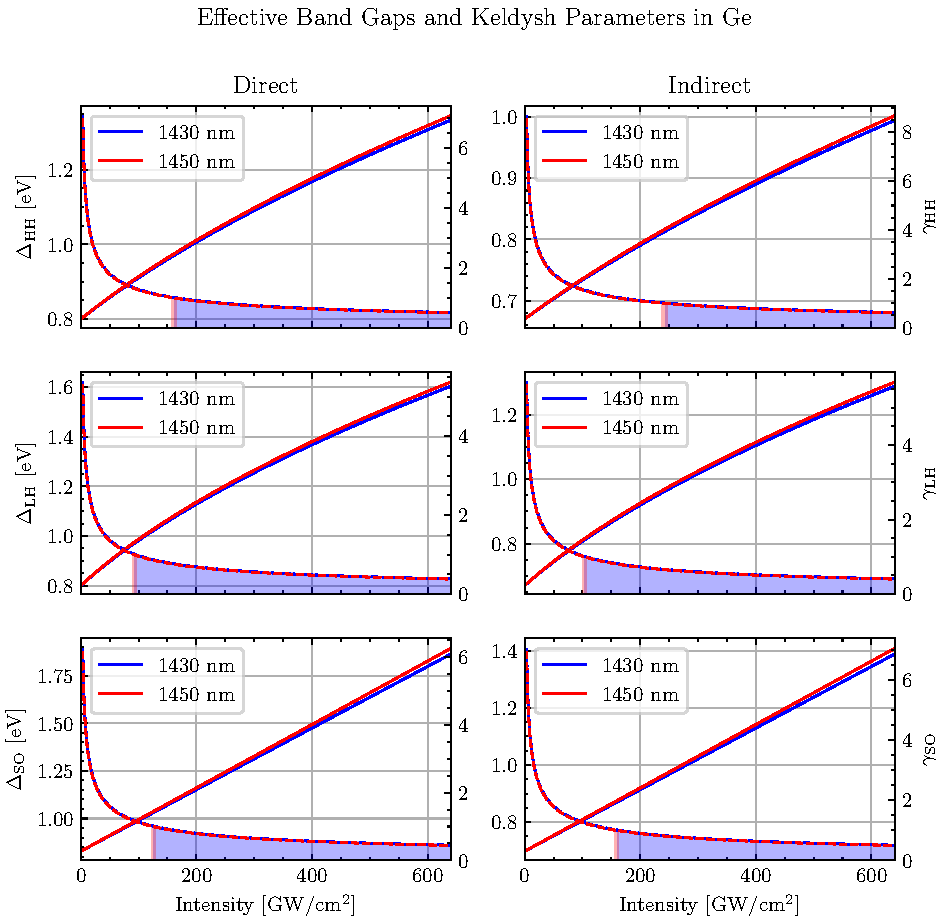
\includegraphics[width=1.0\textwidth]{figures/chap4/Gamma_Gap_Channel_VB_resolved.pdf}
	\caption{Channel- and initial band-resolved effective bandgaps $\Delta_i$ (solid line, left axes) and Keldysh parameters $\gamma_i$ (dashed lines, right axes) as a function of peak intensity. The shaded region under $\gamma_i$ corresponds to intensities where $\gamma_i < 1$ for 1430 nm (blue) and 1450 nm (red).}
	\label{fig:Gamma_Gap_Channel_VB_resolved}
	% plot made with \Python Scripts\DrakeIonization\DrakeIonization.py
\end{figure}

\cref{fig:Gamma_Gap_Channel_VB_resolved} shows the effective band gaps and the Keldysh parameter as a function of peak intensity. The effective bandgap (solid lines, values on left axes) is significant for all initial states and transition types. For example, for a peak intensity of 640 GW/cm\textsuperscript{2} and $\lambda = 1430 \ \textrm{nm}$, the energy required to excite from the light hole band to the conduction band via a direct transition is $\simeq 1.6 \ \textrm{eV}$, which is double the ground state value of 0.8 eV. The dashed lines (values shown on right axis) show the Keldysh parameter $\gamma_i$ for each wavelength. Since $\gamma_i \propto \omega$, the difference between $\gamma_i$ for the two wavelengths is neglible at this scale (about 1.5\%). The shaded region under each $\gamma_i$ curve denotes the intensities at which $\gamma_i<1$. Most intensities resuilt in $\gamma < 1$ or $\gamma \simeq 1$, meaning that both tunnel ionization and multiphoton ionization play an important role. By 250 GW/cm\textsuperscript{2}, $\gamma < 1$ for all possible ionization channels.

%Finally, we convert the excited carrier density to a fractional excitation. Germanium has $N_{\text{u.c.}}=2$ valence electrons per unit cell, and each unit cell has a volume $V_{\text{u.c.}}=4.527 \times 10^{-23} \text{ cm}^{3}$. Therefore the fractional carrier excitation is
%\begin{equation}
%\eta = \Delta N \frac{V_{\text{u.c.}}}{N_{\text{u.c.}}}
%\end{equation}
% NOTE: THIS CONVERSION FACTOR IS WRONG!

% below are the Keldysh ionization rate equations (omitted)
%\begin{equation}
%W_i = \frac{2 \omega}{9 \pi^2} \left( \frac{1}{B} \frac{m \omega}{\hbar} \right)^{3/2} Q\left( \gamma, \frac{\Delta_i^{\textrm{eff}}}{\hbar \omega} \right) \exp \left\{ -\pi \left\langle  \frac{\Delta_i^{\textrm{eff}}}{\hbar \omega} + 1 \right\rangle \times \frac{K(B) - E(B)}{E(A)} \right\}
%\end{equation}
%where we have introduced the shorthand notation:
%\begin{equation}
%\begin{aligned}
%A &= \frac{1}{\sqrt{1+\gamma^2}} \\
%B &= \frac{\gamma}{\sqrt{1+\gamma^2}}
%\end{aligned}
%\end{equation}
%and the function $Q$ is defined as:
%\begin{equation}
%\begin{aligned}
%Q(\gamma, x) &= \left[\pi / 2K(A)\right]^{1/2} \times \sum_{n=0}^{\infty} \left\{-\pi \left[K(B)-E(B)\right] n / E(A) \right\} \\
%&\times \Phi \left\{ \left[\pi^2 \left(2 \langle x+1 \rangle - 2x+n\right) / 2K(A) \times E(A) \right]^{1/2} \right\}
%\end{aligned}
%\end{equation}
%amd the function $\Phi$ is defined as:
%\begin{equation}
%\Phi (z) = ?
%\end{equation}

\subsection{Indirect Transitions}
\label{sec:indirect_transitions}

\begin{figure}
	\centering
	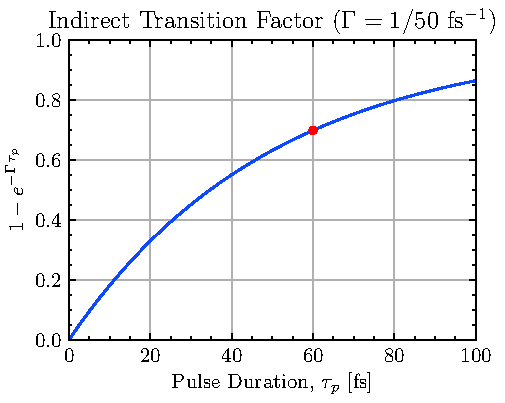
\includegraphics[width=0.75\textwidth]{figures/chap4/Indirect_transition_factor.pdf}
	\caption{Prefactor for indirect transition rates assuming a Poisson distribution. For germanium and a pulse duration of 60 fs, the indirect transition factor is about 0.7. \textbf{NEED TO UPDATE THIS FIGURE WITH NEW PULSE DURATIONS}}
	\label{fig:Indirect_transition_factor}
	% plot made with \Python Scripts\DrakeIonization\DrakeIonization.py
\end{figure}

An indirect transition, where the final crystal momentum is substantially different than its initial value, is mediated by an electron-phonon scattering process. This additional process must occur within the timescale of the laser pulse, and thus we expect the pulse duration and the scattering cross section to impact the relative prevalence of indirect transitions in our experiments. If we assume these collisions occur independent of one another (and, therefore, follow a Poisson distribution), we can calculate the indirect transition ionization rate $W_i^{\textrm{ind.}}$ by multiplying the direct transition rate $W_i^{\textrm{dir.}}$ by a correction factor:
\begin{equation}
W_i^{\textrm{ind.}} = W_i^{\textrm{dir.}} * (1 - \exp(-\Gamma \tau_p))
\label{eqn:Indirect_transition_factor}
\end{equation}
where $\tau_p$ is the pulse duration (\textbf{FWHM OR GUASSIAN PULSE DURATION?}) and $\Gamma$ is the electron-phonon collision rate. The factor in \cref{eqn:Indirect_transition_factor} represents the probability that any given electron will undergo one or more phonon collisions in the time $\tau_p$, assuming the collisions follow a Poisson distribution. For germanium, we estimate $1/\Gamma \approx 47 \ \textrm{fs}$, which is a ballpark figure inferred from measurements of laser-induced periodic surface structures on Ge \cite{austinSemiconductorSurfaceModification2017}. When calculating $W_i^{\textrm{dir.}}$, we use the the local conduction band mass $m_{\textrm{CB}}$ in the indirect valley and the indirect energy gap $\Delta_i^{\textrm{ind.}}$. \cref{fig:Indirect_transition_factor} shows the prefactor in \cref{eqn:Indirect_transition_factor} as a function of pulse duration. \textbf{For our experiment, $\tau_p = 60 \ \textrm{fs}$ and the prefactor evaluates to $\sim 0.72$.} We note that a shorter pulse duration of $\sim 12 \ \textrm{fs}$, which is achievable with our lab's fiber compressor \cite{zhangAtomicMolecularDynamics2015}, would give a prefactor of $\sim 0.23$.

\subsection{Spectral Content of the Laser Pulse}
\label{sec:bandwidth_of_pulse}

\begin{figure}
	\centering
	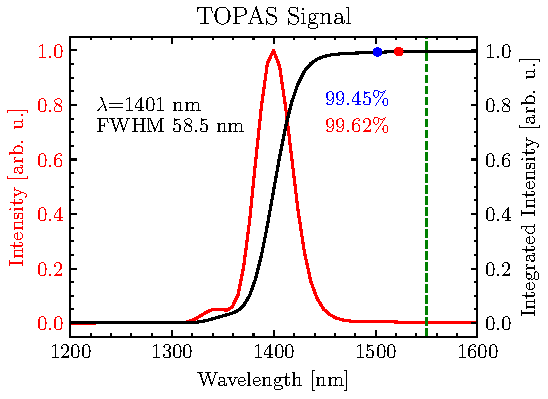
\includegraphics[width=0.75\textwidth]{figures/chap4/TOPAS_1400nm_spectral_inten.pdf}
	\caption{TOPAS spectral content at $\lambda = 1401 \ \textrm{nm}$.}
	\label{fig:TOPAS_1400nm_spectral_inten}
	% figure made in \Python Scripts\FROG\FROG2.py
\end{figure}

Since we are near the bandgap ($\Delta^{\textrm{dir.}} = 1550 \ \textrm{nm}$, $\Delta^{\textrm{ind.}} = 1879 \ \textrm{nm}$), it's possible that a portion of the IR pulse's spectrum will be below the bandgap, which would have consequences for both the interference and Keldysh calculations. \cref{fig:TOPAS_1400nm_spectral_inten} shows the spectral content of the TOPAS when it is set to 1400 nm.\footnote{Unfortunately, we did not measure the spectral content of the pulse when the TOPAS was set at $\lambda = 1430$ or 1450 nm. However, in our experience the shape of the spectral envelope is invariant under small wavelength shifts.} We will use this spectrum to estimate the spectral content when operating at 1430 and 1450 nm. The red line shows the spectral intensity, the black line is the integrated sum of the red line, and the green dashed vertical line represents the direct bandgap. When the TOPAS is operating at 1430 nm (1450 nm), the central wavelength $\lambda_0$ is 120 nm (100 nm) above the bandgap. According to this measurement, when the TOPAS is running at 1400 nm, 99.45\% of the pulse energy is at wavelengths below the $\lambda_0 + 100 \ \textrm{nm}$ (blue dot), and 99.62\% of the pulse energy is at wavelengths below $\lambda_0 + 120 \ \textrm{nm}$ (red dot). If we assume the spectral envelope is invariant under small wavelength shifts, then it stands to reason that when the TOPAS is run at 1430 or 1450 nm, over 99\% of the pulse energy is above Ge's bandgap (1550 nm). Thus, we are justified in treating the pulse as if it were entirely above the band gap.

\subsection{Keldysh Results}
\label{sec:nonlinear_excitation_results}

We now present the ionization results of the model introduced in \cref{sec:nonlinear_excitation_model_details,sec:indirect_transitions}. We start with single-intensity calculations (i.e., what we would observe if we had a $\delta$-function intensity distribution in \cref{fig:TMM_hist_chrom_int_2x2}), then proceed to focal volume average the results using the IR intensity distributions in \cref{sec:thin_film_interference} and \cref{fig:pump_on_focus_calculation}. Focal volume-averaged results are presented in \cref{sec:volume_averaging}.

The simulation was performed for two wavelengths ($\lambda = 1430, 1450 \ \textrm{nm}$) and 1000 different peak intensities, ranging from 3.26 to 640 GW/cm\textsuperscript{2}. A Gaussian pulse envelope was assumed with a pulse duration of $\tau_p = 60 \ \textrm{fs}$, and the time relative to the center of the pulse $\tau$ ranged from -120 to +120 fs in 1000 steps. For each set of input parameters, the simulation outputs an initial band- (HH, LH, SO) and transition type- (indirect, direct) resolved electron population in the conduction band as a function of $\tau$.

\begin{figure}
	\centering
	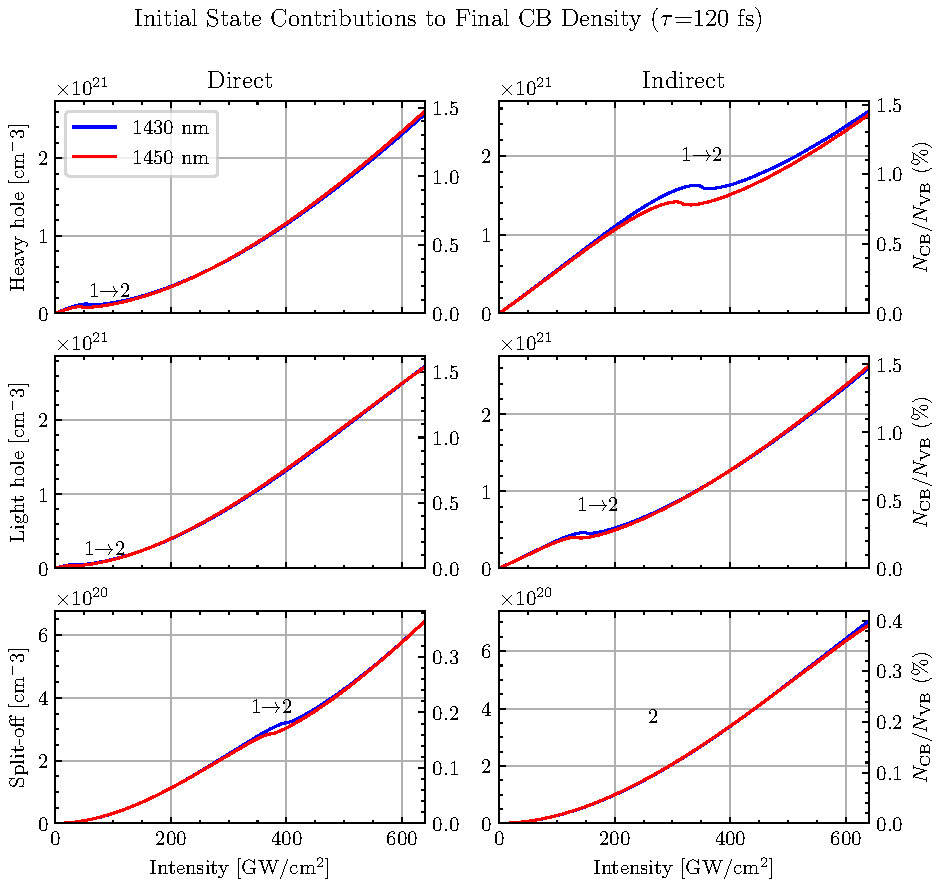
\includegraphics[width=1.0\textwidth]{figures/chap4/N_Channel_VB_resolved.pdf}
	\caption{Transition type and initial band resolved contributions to the final conduction band density. Inset text denotes the values of $n_i$ at the peak intensity (for $\tau=0$ fs) as the minimum number of photons required to excite the electron across the gap increases by 1.}
	\label{fig:N_Channel_VB_resolved}
	% plot made with \Python Scripts\DrakeIonization\DrakeIonization.py
\end{figure}

\cref{fig:N_Channel_VB_resolved} shows the main result of the Keldysh calculation. We plot the contributions from each ionization channel (direct \& indirect) and for each of the three initial bands after the IR pulse has left ($\tau = 120 \ \textrm{fs}$) as a function of peak intensity. We see an intensity-dependent effect where $N_{\textrm{CB}}$ has a local maximum, a slight dip, and then an increase. At this scale, this feature is most prominent in for indirect heavy hole plot, but the general shape is the same for all channels. These features occur at intensities that coincide with an increase in the minimum number of photons required to cross the bandgap ($n_i$ in \cref{eqn:min_number_photons}), akin to channel-closure \cite{shcheblanovNonlinearPhotoionizationTransparent2017}. The value of $n_i$ is denoted in the plot on either side of the feature.
%We interpret this as a result of the effective bandgap changing with increasing field strength (see \cref{eqn:eff_bandgap_HHLL,eqn:eff_bandgap_SO}).

\begin{figure}
	\centering
	\includegraphics[width=0.75\textwidth]{figures/chap4/Total_CB_dens_vs_Time.pdf}
	\caption{Total valence band (VB) population as a function of laser pulse delay. Inset shows the pulse envelope.}
	\label{fig:Total_CB_dens_vs_Time}
	% plot made with \Python Scripts\DrakeIonization\DrakeIonization.py
\end{figure}

\cref{fig:Total_CB_dens_vs_Time} shows the total excitation (summed over all channels and initial bands) of the sample as a function of $\tau$ for the highest intensity ($I = 640$ GW/\textsuperscript{2}). The result is a modified error function, owing to the nonlinearity of the sample's response. We see there is little difference between the two wavelengths in terms of total excitation. Because we use the pulse envelope, rather than the instantenous field strength, we do not see steps in the ionization fraction every half-period \cite{schultzeAttosecondBandgapDynamics2014}.

\begin{figure}
	\centering
	\includegraphics[width=0.75\textwidth]{figures/chap4/CB_dens_vs_Int.pdf}
	\caption{Contributions of the initial bands to the final conduction band (CB) density at the end of the pulse ($\tau = \infty$). Dark lines are for $\lambda = 1430 \ \textrm{nm}$, faint lines are for $\lambda = 1450 \ \textrm{nm}$.}
	\label{fig:CB_dens_vs_Int}
	% plot made with \Python Scripts\DrakeIonization\DrakeIonization.py
\end{figure}

\cref{fig:CB_dens_vs_Int} shows the population of the conduction band after the IR pulse has left (${\tau = 120 \ \textrm{fs}}$) as a function of peak intensity. For all intensities, the signal is dominated by contributions by the heavy and light holes, which is to be expected as the split-off band has a higher ionization potential. For 1430 nm, we see that at 160 GW/cm\textsuperscript{2}, the heavy hole VB is responsible for about 50.2\% of the CB population, followed by the light hole VB at around 31.8\%, and finally the split-off VB at around 18.0\% percent, with similar ratios for 1450 nm. Above 400 GW/cm\textsuperscript{2}, the LH contribution begins to overtake the HH. In our experience, a peak intensity of above 640 GW/cm\textsuperscript{2} corresponds to immediate sample damage, meaning that we can expect no more than $1.32 \times 10^{22} \textrm{cm}^{-3} \simeq 7.5\% \ N_{\textrm{VB}}$ fractional excitation in our experiments. This indicates that ultrafast melting should not be a concern below 640 GW/cm\textsuperscript{2}.

\begin{figure}
	\centering
	\includegraphics[width=0.75\textwidth]{figures/chap4/Direct_vs_Indirect_Trans.pdf}
	\caption{Contributions by indirect and direct transitions to the final conduction band (CB) density at the end of the pulse ($\tau = \infty$). Dark lines are for $\lambda = 1430 \ \textrm{nm}$, faint lines are for $\lambda = 1450 \ \textrm{nm}$.}
	\label{fig:Direct_vs_Indirect_Trans}
	% plot made with \Python Scripts\DrakeIonization\DrakeIonization.py
\end{figure}

\cref{fig:Direct_vs_Indirect_Trans} shows the relative contribution of indirect and direct transitions to the total population density by the end of the pulse as a function of peak intensity. Recalling \cref{eqn:Indirect_transition_factor}, the indirect transition rate is suppressed due to the product $\tau_p \Gamma \approx 0.7$. However, this factor is not enough to overcome the relative increase in ionization due to the lower bandgap of the indirect transition compared to the direct transition. Consequently, only {20 - 50\%} of the excited population are due to direct transitions. At the highest intensities, we see equal contributions by both channels.

\textbf{question}: which electron populations are we sensitive to in our measurement?

The above calculations assume a single peak intensity throughout the sample, but a spatially invariant intensity profile is unphysical. In a real experiment, the sample experiences a spatially varying intensity profile, which results in a nonuniform excitation fraction. We have already addressed the diffraction-induced transverse intensity profile of the IR focus (see \cref{sec:Pump_Arm_Focus_Calculations}). In the following section, we will calculate the intensity profile along the direction of propagation within the sample.

\subsection{Thin Film Interference Calculations}
\label{sec:thin_film_interference}

%\begin{figure}
%	\centering
%	\subfloat[]{
%		\includegraphics[width=0.75\textwidth]{figures/chap4/GeSiN_RAT_1430nm.pdf}
%		\label{fig:GeSiN_RAT_1430nm}}
%	
%	\subfloat[]{
%		\includegraphics[width=0.75\textwidth]{figures/chap4/GeSiN_RAT_1450nm.pdf}
%		\label{fig:GeSiN_RAT_1450nm}}
%	\caption{Thin film calculations for the sample heterostructure for $\lambda = 1430 \ \textrm{nm}$ and $1450 \ \textrm{nm}$. The red region represents germanium; green is silicon nitride; white is vacuum. The top panel shows the absorbed energy density per unit input power. The bottom panel shows the local intensity $S(z) \equiv \vb{S}(z) \vdot \hat{z}$, normalized by the input intensity $S(0) \equiv \vb{S}(0) \vdot \hat{z}$. See text for details.}
%	\label{fig:GeSiN_RAT:both}
%	% python script: \Python Scripts\thinfilm\thinfilm.py
%\end{figure}

The sample is a heterostructure of 100 nm germanium ($\tilde{n} = 4.2481 + 0.066041i$ at 1430 nm) on a 30 nm silicon nitride membrane ($\tilde{n}=1.9997 + 0i$ at 1430 nm) with a total thickness measuring $\sim 9$\% of the fundamental wavelength. As a result, we cannot ignore thin film interference effects that may arise from this geometry. To account for this, we calculated the intensity profile in the heterostructure for the two wavelengths of experimental interest (1430 and 1450 nm) using the transfer matrix method. We also calculate the intensity profile with the assumption that there is no internal interference pattern. As will be shown below, these two methods result in drastically different intensity profiles. The actual internal profile is likely somewhere between the two, as the sample is not an ideal thin film, nor is its quality so poor that it is completely incapable of supporting interference patterns. The resulting intensity profiles are later used as inputs to the Keldysh nonlinear photoionization code. Refractive index data for germanium \cite{nunleyOpticalConstantsGermanium2016} and the silicon nitride \cite{lukeBroadbandMidinfraredFrequency2015} were taken from the literature. Calculations were performed using the \textit{TMM package for Python} \cite{byrnesTmmSimulateLight2017,byrnesMultilayerOpticalCalculations2019}.

The TMM code assumes a multilayer planar stack of non-magnetic ($\mu = \mu_0$) and isotropic materials. The interfaces are considered ideal (i.e., zero surface roughness), so this result represents an upper limit on the interference effects present in our system. Nonlinear effects are excluded from this calculation. The electric field is expressed as a superposition of forward- and backward-propagating complex-valued waves:
\begin{equation}
\begin{aligned}
\vb{E}(\vb{r}) &= \vb{E}_f^0 \exp(i \vb{k}_f \vdot \vb{r}) + \vb{E}_b^0 \exp(i \vb{k}_b \vdot \vb{r}), \\
\vb{k}_f &= \frac{2 \pi n}{\lambda_{\textrm{vac}}} \left( \vu{z} \cos \theta + \vu{x} \sin \theta \right), \\
\vb{k}_b &= \frac{2 \pi n}{\lambda_{\textrm{vac}}} \left( - \vu{z} \cos \theta + \vu{x} \sin \theta \right),
\end{aligned}
\end{equation}
where $\theta$ is the angle between $\vb{k}$ and the surface normal. The code solves for the internal complex electric field by applying the transfer matrix method to the heterostructure assuming an input electric field of unit magnitude \cite{nistadCausalityElectromagneticProperties2008,harbeckeCoherentIncoherentReflection1986,ohtaMatrixFormalismCalculation1990,katsidisGeneralTransfermatrixMethod2002,shalabneyElectromagneticFieldsDistribution2010}. We obtain the physical field at any time $t$ by multiplying the complex field by $e^{-i \omega t}$ and taking the real part of the resulting expression. We define the \textit{peak normalized intensity} as the local peak intensity divided by the peak intensity in the absence of the heterostructure\footnote{We omit the denominator as it evaluates to unity with an input field of unit strength. That is, $\textrm{max}_{t}\left( \left|\sum_{\lambda}\vb{E}_{\textrm{vac.},\lambda}\right|^2 \right) = 1$.}:
\begin{equation}
\frac{I_p(z)}{I_{p,0}(z)} \equiv \Re{\tilde{n}_{\lambda_0}(z)} \ \textrm{max}_{t}\left(\left|\sum_{\lambda}\vb{E}_\lambda(z, t)\right|^2 \right)
\end{equation}
where $\tilde{n}_{\lambda_0}(z)$ is complex refractive index at the central wavelength at position $z$. The normalized peak intensity will later be used to convert vacuum intensities to sample intensities. We also report the transmitted ($T$), reflected ($R$) and absorbed power ($A$) of the heterostructure.

\begin{figure}
	\centering
	\includegraphics[width=0.9\textwidth]{figures/chap4/tmm_vs_WL_1200-1600nm.pdf}
	\caption{Optical properties of the Ge/SiN heterostructure and a freestanding 100 nm Ge membrane as a function of wavelength. For the $R$, $A$ and $T$ panels, solid lines represent the coherent calculations, and dashed lines represent the incoherent calculations. TMM calculations assume monochromatic light.}
	\label{fig:tmm_vs_WL_1200-1600nm}
\end{figure}

We start by considering the wavelength dependence of the calculated optical properties. The top left panel of \cref{fig:tmm_vs_WL_1200-1600nm} shows the complex refractive index of germanium and silicon nitride over the range 1200 -- 1600 nm. Note that the vertical scale for k(Ge) has been enlarged for visual clarity. In the following discussion, we consider either a heterostructure (germanium sample at {$z$ = 0 -- 100 nm}, silicon nitride at {$z$ = 100 -- 130 nm}, and vacuum elsewhere) or a freestanding germanium film (germanium sample at {$z$ = 0 -- 100 nm}, and vacuum elsewhere). The IR laser propagates in the $+z$ direction with a normal incidence angle ($\theta = 0$). The refractive index for silicon nitride is effectively constant over this range, and germanium's index is well-behaved below 1520 nm (near the direct bandgap at 1550 nm). The solid lines in the remaining three panels of \cref{fig:tmm_vs_WL_1200-1600nm} show the transmitted, reflected and absorbed power for both a freestanding 100 nm Ge film and a 100 nm Ge / 30 nm SiN hetereostructure assuming full coherence of the beam. The dashed lines in these panels show the results of an \textit{incoherent TMM calculation}, in which we discard the phase information of the light to approximate the effects of a rough surface or spatially varying film thickness.

As should be expected, interference effects are critical to understanding the optical properties when the structure is sub-wavelength. The coherence is responsible for nearly doubling the reflectance and reducing the absorbed power by a factor of $\approx 2.5$ at 1400 nm.  We can see that the reflected and transmitted power do not change appreciably over the range {1400 -- 1500 nm}, which encompasses the spectral envelope of a TOPAS signal centered at 1430 or 1450 nm. For both the hetereostructure and the freestanding Ge film, about 75 percent of the incident power is reflected, about 23 percent is transmitted, and about 2 percent is linearly absorbed.

We note that at these wavelengths the coherence length, $L$, greatly exceeds the sample thickness \cite{katsidisGeneralTransfermatrixMethod2002}:
\begin{equation}
L = \frac{\lambda^2}{n \Delta \lambda}
\end{equation}
For a laser pulse with a central wavelength of 1430 nm and a bandwidth of 58.5 nm, $L(\textrm{Ge}) \approx 8.23 \ \mu\textrm{m}$ and $L(\textrm{SiN}) \approx 17.4 \ \mu\textrm{m}$, which is $\approx 80$ and $\approx 580$ times longer than the thickness of the germanium and silicon nitride films, respectively. We also note that a round trip reflection within the heterostructure will take 3.2 fs at 1430 nm, which is 18 times shorter than the laser pulse. For these reasons, we use standard interference calculation methods to estimate the intensity profile within the heterostructure.
%Additionally, we can quantify the effect of the SiN membrane, which was required due to the technical limitations of our sample preparation process.

%We also report the normalized absorbed energy density, $a(z)$:
%\begin{equation}
%a(z) = \frac{\left|E_f + E_b \right|^2 \Im \left[n \cos(\theta) k_z\right]}{\Re \left[ n_0 \cos \theta_0 \right]},
%\end{equation}
%where the zero subscript denotes the quantity in vacuum. We also calculate the peak normalized intensity, $I_p(z) / I_{p,0}(z)$, which is the local peak intensity divided by the peak intensity in the absence of the heterostructure. The transmitted ($T$), reflected ($R$) and absorbed power ($A$) of the heterostructure are also reported. 
%For $s$-polarized light, the normal component of the Poynting vector $\vb{S} \vdot \vu{z}$ at position $z$ can be written as:
%\begin{equation}
%S(z) \equiv \vb{S} \vdot \vu{z} = \frac{1}{2} \Re \left[ \vu{z} \vdot (\vb{E^*} \cp \vb{H}) \right] \ \propto \Re \left[ (E_f^* + E_b^*)(E_f-E_b) n \cos \theta \right],
%\end{equation}
%where $E_f$ ($E_b$) is the forward (backward) amplitude evaluated at position $z$. We report this quantity normalized by the normal component of the incident Poynting vector that would result from the absence of the heterostructure ($\vb{S} \vdot \vu{z}$  with $E_b = 0$ and $E_f = 1$):
%\begin{equation}
%\frac{S(z)}{S(0)} = \frac{\Re \left[ (E_f^* + E_b^*)(E_f-E_b) n \cos \theta \right]}{\Re \left[n_0 \cos \theta_0 \right]},
%\end{equation}
%where the zero subscript denotes the quantity in vacuum.
%\begin{figure}
%	\centering
%	\subfloat[]{
%		\includegraphics[width=0.75\textwidth]{figures/chap4/TMM_1430_1450_RAT.pdf}
%		\label{fig:TMM_1430_1450_RAT}}
%	
%	\subfloat[]{
%		\includegraphics[width=0.75\textwidth]{figures/chap4/TMM_1430_1450_Geonly_RAT.pdf}
%		\label{fig:TMM_1430_1450_Geonly_RAT}}
%	\caption{Thin film calculations at $\lambda = 1430 \ \textrm{nm}$ and $1450 \ \textrm{nm}$ for (a): {100 nm} Ge film on a {30 nm} SiN membrane and (b): {100 nm} freestanding Ge membrane. The red region represents germanium; green is silicon nitride; white is vacuum. See text for details.}
%	\label{fig:GeSiN_RAT:both}
%	% python script: \Python Scripts\thinfilm\thinfilm.py
%\end{figure}
\begin{figure}
	\centering
	\includegraphics[width=0.75\textwidth]{figures/chap4/TMM_1430_1450_broad_Int.pdf}
	\caption{Broadband TMM calculations for a {100 nm} Ge film and {30 nm} SiN membrane. The red region represents Ge; green is SiN; white is vacuum. Solid lines are TMM results, dashed lines are \cref{eqn:Iint_fresnel_losses}.}
	\label{fig:TMM_1430_1450_broad_Int}
	% python script: \Python Scripts\thinfilm\thinfilm.py
\end{figure}
%\begin{figure}
%	\centering
%	\includegraphics[width=0.75\textwidth]{figures/chap4/TMM_1430_1450_RAT_a_Int.pdf}
%	\caption{TMM calculations for a {100 nm} Ge film and {30 nm} SiN membrane. The red region represents Ge; green is SiN; white is vacuum. See text for details.}
%	\label{fig:TMM_1430_1450_RAT_a_Int}
%	% python script: \Python Scripts\thinfilm\thinfilm.py
%\end{figure}
%\begin{figure}
%	\centering
%	\includegraphics[width=0.75\textwidth]{figures/chap4/TMM_1430_1450_RAT.pdf}
%	\caption{Thin film calculations for the sample heterostructure for $\lambda = 1430 \ \textrm{nm}$ and $1450 \ \textrm{nm}$. The red region represents germanium; green is silicon nitride; white is vacuum. The top panel shows the absorbed energy density per unit input power. The bottom panel shows the normal component of the Poynting vector, normalized by the incident intensity. See text for details.}
%	\label{fig:TMM_1430_1450_RAT}
%	% python script: \Python Scripts\thinfilm\thinfilm.py
%\end{figure}

Since the TMM model is linear, we can extend it to handle a broadband pulse by coherently summing the resulting electric field over the bandwidth of the pulse. Broadband TMM calculations were performed using $N=500$ monochromatic TMM calculations over the spectral range 1300 - 1500 nm. Spectral weights for each wavelength were calculated by interpolating the square root of the spectral intensity in \cref{fig:TOPAS_1400nm_spectral_inten} after shifting the spectral envelope to the appropriate central wavelength.

We compare the TMM result to a simpler model which only includes Fresnel losses from the front interface (vacuum-Ge) and linear absorption thereafter \cite{zurchDirectSimultaneousObservation2017}:
\begin{equation}
\frac{I_p(z)}{I_{p,0}(z)} = \Re{\tilde{n}} \left| \frac{2}{1+\tilde{n}} \right|^2 \exp \left[ - \left( \frac{4 \pi}{\lambda_0} \right) \Im{\tilde{n}} z \right] \approx 0.60,
\label{eqn:Iint_fresnel_losses}
\end{equation}
where $\tilde{n}$ is the complex refractive index of Ge evaluated at the central wavelength of the pulse ($\lambda_0$) and $z$ is the depth within the Ge sample. While this method does not calculate the intensity profile outside of the germanium, we note that this information is superfluous as SiN's large band gap ($\Delta \approx 5 \ \textrm{eV}$) precludes any linear absorption, and our XUV measurement is insensitive to any dynamics occuring within the SiN membrane.

\cref{fig:TMM_1430_1450_broad_Int} shows the calculated peak normalized intensity profile of a heterostructure consisting of 100 nm of germanium on a 30 nm thick silicon nitride membrane for $\lambda = 1430$ and 1450 nm. The solid lines are broadband TMM calculations, and the dashed lines are the Fresnel absorption model (\cref{eqn:Iint_fresnel_losses}). Starting with the TMM result, we note that the discrete jumps in intensity at the sample boundaries are due to the discrete jumps in the refractive index. Inside the Ge, we see a strong modulation of the intensity due to interference effects. Before the sample ($z < 0$), the intensity is suppressed by the coherent back reflection from the vacuum-Ge interface. Inside the sample, the intensity has a minimum about 20 nm below the vacuum-Ge interface. From $z=20 \ \textrm{nm}$ to $z=80 \ \textrm{nm}$ the normalized peak intensity increases linearly before asymtoptically approaching a maximum value at the Ge-SiN boundary. Therefore, the broadband TMM model predicts that the highest intensities are located on the back face of the Ge sample, which can be understood as a combined reflection off the Ge-SiN and SiN-vacuum interfaces. In contrast to the TMM result, \cref{eqn:Iint_fresnel_losses} yields an intensity profile that is very nearly linear over the limited 100 nm distance. In either model, changing the wavelength from 1430 nm to 1450 nm does not appreciably change the intensity profile.

%\begin{figure}
%	\centering
%	\includegraphics[width=0.75\textwidth]{figures/chap4/GeOnly_1430_1450_RAT_a_Int.pdf}
%	\caption{TMM calculations for a {100 nm} freestanding Ge thin film. The red region represents Ge; white is vacuum. See text for details.}
%	\label{fig:GeOnly_1430_1450_RAT_a_Int}
%	% python script: \Python Scripts\thinfilm\thinfilm.py
%\end{figure}
\begin{figure}
	\centering
	\includegraphics[width=0.75\textwidth]{figures/chap4/Ge_1430_1450_broad_Int.pdf}
	\caption{Broadband TMM calculations for a {100 nm} freestanding Ge thin film. The red region represents Ge; white is vacuum. Solid lines are TMM results, dashed lines are \cref{eqn:Iint_fresnel_losses}.}
	\label{fig:Ge_1430_1450_broad_Int}
	% python script: \Python Scripts\thinfilm\thinfilm.py
\end{figure}

The presence of the silicon nitride membrane was required for technical materials preparation reasons. To quantify the effect of its presence on the internal intensity distribution, we performed broadband TMM calculations for a 100 nm thick freestanding germanium membrane, as shown in \cref{fig:Ge_1430_1450_broad_Int}. Comparing it to the previous result, we can see that the addition of the SiN membrane does not significantly change the optical properties of the sample, as the general shape of the intensity profile is the same as the heterostructure. By adding the SiN membrane, reflectivity increases by $\approx 2.5\%$, absorption decreases by $\approx 4.2\%$, and transmission increases by $\approx 9.6\%$. The increased reflection losses are not a concern, as we have sufficient flux in our pump arm to make up for the increased losses. The dashed lines show \cref{eqn:Iint_fresnel_losses}, which does not take into account the presence or absence of the SiN membrane and is the same as in \cref{fig:TMM_1430_1450_broad_Int}.

If the sample response was strictly linear, then the measured ATAS signal should be proportional to the average intensity within the XUV probe. For the Ge/SiN heterostructure, the average intensity of the TMM model is about 65\% that of the Fresnel model. On the other hand, a nonlinear sample response gives the higher intensity regions outsized importance, and we see that the broadband TMM interference pattern has a maximum intensity 50\% higher than the Fresnel model. These numbers are similar for the freestanding germanium geometry, albeit less pronounced (average intensity TMM:average intensity Frensel = 0.68, maximum intensity TMM:maximum intensity Fresnel = 0.44).

\begin{table}[]
	\centering
	\begin{tabular}{l|l|l|l|l}
		\textbf{TMM Type} &
		\textbf{Structure} &
		\textbf{$\lambda_0$ {[}nm{]}} &
		\textbf{min$\left(\frac{I_p(z)}{I_{p,0}(z)}\right)$ {[}\%{]}} &
		\textbf{max$\left(\frac{I_p(z)}{I_{p,0}(z)}\right)$ {[}\%{]}} \\ \hline
		\multirow{4}{*}{monochromatic} & \multirow{2}{*}{Ge/SiN}          & 1430 & 6.62 & 92.62 \\
		&                                  & 1450 & 6.49 & 91.24\\ \cline{2-5} 
		& \multirow{2}{*}{freestanding Ge} & 1430 & 5.93 & 88.50 \\
		&                                  & 1450 & 5.86 & 87.53 \\ \hline
		\multirow{4}{*}{broadband}     & \multirow{2}{*}{Ge/SiN}          & 1430 & 6.68 & 92.19 \\
		&                                  & 1450 & 6.53 & 90.90 \\ \cline{2-5} 
		& \multirow{2}{*}{freestanding Ge} & 1430 & 6.01 & 88.67 \\
		&                                  & 1450 & 5.90 & 87.84
	\end{tabular}
	\caption{TMM calculated internal intensity ranges for a 100 nm Ge / 30 nm SiN heterostructure and a freestanding Ge film.}
	\label{tab:TMM_intensity_range}
\end{table}
%\begin{table}[]
%	\centering
%	\begin{tabular}{l|l|l|l|l}
%		\textbf{TMM Type} &
%		\textbf{Structure} &
%		\textbf{$\lambda_0$ {[}nm{]}} &
%		\textbf{min$\left(\frac{I_p(z)}{I_{p,0}(z)}\right)$ {[}\%{]}} &
%		\textbf{max$\left(\frac{I_p(z)}{I_{p,0}(z)}\right)$ {[}\%{]}} \\ \hline
%		\multirow{4}{*}{\textbf{monochromatic}} & \multirow{2}{*}{Ge/SiN}          & 1430 & 1.56 & 21.70 \\
%		&                                  & 1450 & 1.53 & 21.40 \\ \cline{2-5} 
%		& \multirow{2}{*}{freestanding Ge} & 1430 & 1.40 & 20.80 \\
%		&                                  & 1450 & 1.38 & 20.60 \\ \hline
%		\multirow{4}{*}{\textbf{broadband}}     & \multirow{2}{*}{Ge/SiN}          & 1430 & 1.57 & 21.60 \\
%		&                                  & 1450 & 1.54 & 21.32 \\ \cline{2-5} 
%		& \multirow{2}{*}{freestanding Ge} & 1430 & 1.42 & 20.84 \\
%		&                                  & 1450 & 1.39 & 20.65
%	\end{tabular}
%	\caption{TMM calculated internal intensity ranges for a 100 nm Ge / 30 nm SiN heterostructure and a freestanding Ge film. See text for details.}
%	\label{tab:TMM_intensity_range}
%\end{table}

A simple monochromatic TMM calculation at the central wavelength of the pulse can reveal much of the same information in a fraction of the computational time. \cref{tab:TMM_intensity_range} shows intensity extrema for the different sample geometries, wavelengths and TMM calculation methods. For our relatively narrow bandwidth, including the coherent sum over all wavelengths changes the results by about 1\%. Not shown are the monochromatic versions of \cref{fig:TMM_1430_1450_broad_Int,fig:Ge_1430_1450_broad_Int}, but the differences between the two methods are imperceptible at this scale.

\begin{figure}
	\centering
	\includegraphics[width=0.75\textwidth]{figures/chap4/TMM_hist_chrom_int_2x2.pdf}
	\caption{Calculated intensity distributions in Ge/SiN heterostructures and Ge thin films. Dark colors follow broadband TMM calculations, light colors follow \cref{eqn:Iint_fresnel_losses}.}
	\label{fig:TMM_hist_chrom_int_2x2}
	% python script: \Python Scripts\thinfilm\thinfilm.py
\end{figure}

The distribution of intensities within the sample is important when calculating the focal volume averaged Keldysh ionization, and anything short of a $\delta$-function distribution of intensities will smear out intensity-dependent effects. \cref{fig:TMM_hist_chrom_int_2x2} shows histograms ($N = 40$ bins) of the intensity distributions of the aforementioned sample geometries and experimental conditions. The dark colors are the results of the broadband TMM calculation, and the lighter colors follow from \cref{eqn:Iint_fresnel_losses}. The general shape of the TMM's distribution is similar for both wavelengths and sample geometries. In all four cases, most of the sample sees relatively low intensities ($<20\%$ of the incident intensity), whereas on the volume closest to the rear face of the stack experiences high intensities ($>75\%$ of the incident intensity). The distribution is flat for intermediate intensities ({20 -- 75 \%} of the incident intensity), owing to the linear increase of intensity with increasing $z$. It should be noted that the high-intensity tail of the freestanding Ge samples is slightly more pronounced than the Ge/SiN heterostructures, which could facilitate the measurement of intensity-dependent effects. In contrast, the Fresnel absorption model (\cref{eqn:Iint_fresnel_losses}) predicts a near-$\delta$ function intensity distribution.

These calculations were run over a range of incident angles. The resulting intensity distribution does not appreciably change for either s- or p-polarized light if the incident angle remains below 20 degrees (measured from normal). We did not carefully control for the incident angle when installing our samples, but since this result is not sensitive to the incident angle, it is reasonable to assume that our sample experiences the intensity distribution shown in \cref{fig:TMM_hist_chrom_int_2x2}.
%for TMM results vs. incident angle, see the code block at end of thinfilm.py. I did not save these results to disk.

Having computed the intensity profile within the Ge sample, we can now apply the Keldysh model to our experiment.

\subsection{Volume Averaging}
\label{sec:volume_averaging}

We calculate the intensity inside the sample as the product of the sample-free vacuum intensity $I_{\textrm{vac.}}$, the transverse diffraction-induced term $I_{\textrm{diff.}}(x, y)$ (\cref{fig:pump_on_focus_calculation}) and the interference/absorption term $I_p(z) / I_{p,0}(z)$ (\cref{sec:thin_film_interference}):

\begin{equation}
I_{\textrm{sample}}(x, y, z, \tau) \equiv I_{\textrm{vac.}}(\tau) \times I_{\textrm{diff.}}(x, y) \times \frac{I_p(z)}{I_{p,0}(z)}
\label{eqn:sample_intensity_XYZtau}
\end{equation}

We provide a brief summary of the aforementioned profiles here. Combining the first two terms, $I_{\textrm{vac.}} \times I_{\textrm{diff.}}$ has a peak intensity at the focus of $\approx 2.3 \times 10^{11}$ W/cm\textsuperscript{2} per 1 $\mu$J input energy (as measured before lens L4), and $I_p(z) / I_{p,0}(z)$ has a maximum value of about 93\% (for a Ge/SiN heterostructure). Therefore, the maximum peak intensity in the germanium sample is approximately $2.13 \times 10^{11}$ W/cm\textsuperscript{2} per 1 $\mu$J input energy. 

\begin{figure}
	\centering
	\includegraphics[width=0.75\textwidth]{figures/chap4/excitation_at_focus.pdf}
	\caption{Cross sectional slice of the IR intensity profile, XUV intensity profile and total excited state fraction at the rear of the Ge sample in a Ge/SiN heterostructure and the center of the IR pulse ($\tau = 0 \ \textrm{fs}$). The IR intensity profile follows from a broadband TMM calculation for a 100 nm Ge / 30 nm SiN hetereostructure and an input pulse energy of 2.85 $\mu$J of $\lambda = 1430 \ \textrm{nm}$.}
	\label{fig:excitation_at_focus}
	% plot made with \Python Scripts\DrakeIonization\VolumeAveraging_class_script.py
\end{figure}

We map the Keldysh simulation result $N_{\textrm{CB}}(I, \tau)$ onto the intensity distribution $I_{\textrm{sample}}(x, y, z, \tau)$ to get the conduction band electron density distribution $N_{\textrm{CB}}(x, y, z, \tau)$ within the sample. \cref{fig:excitation_at_focus} shows an example lineout of the IR intensity and the conduction band electron density in our sample. This slice was taken at the Ge/SiN interface ($z=100$ nm) at the peak of the pulse ($\tau=0$ fs), where the intensity is the highest. We see that the excitation (blue solid line) mostly follows the Airy-like diffraction pattern of the IR intensity (red dashed line). Deviations between the two profiles are due to the nonlinear response of the sample to the laser. The XUV profile is also shown (black solid line) in arbitrary units, which will be used to perform the volume averaging integral, \cref{eqn:Delta_A_3}.

\begin{figure}
	\centering
	\includegraphics[width=0.75\textwidth]{figures/chap4/FVA_XUV_signal.pdf}
	\caption{Calculated final $\Delta A$ as a function of input pulse energy. These curves were calculated using $\alpha_{10}(32 \ \textrm{eV})$ (absorption).}
	\label{fig:FVA_XUV_signal}
	% plot made with \Python Scripts\DrakeIonization\VolumeAveraging_class_script.py
\end{figure}

\cref{fig:FVA_XUV_signal} shows the intensity scaling of the focal volume averaged $\Delta A$ for the three different intensity profiles. There is little difference between the Ge/SiN heterostructure and freestanding results, which follows from their simliar internal intensity profiles. This confirms our suspiscion that the SiN membrane does not strongly affect the experimental results. On the contrary, the simple Fresnel absorption model has a narrow intensity distribution, and as a result the intensity-dependent features persist through the volume averaging. The higher average intensity of the Fresnel absorption model results in a signal that is about 40\% higher than either TMM intensity distribution.

\begin{figure}
	\centering
	\includegraphics[width=0.75\textwidth]{figures/chap4/FVA_Total_CB_dens_vs_T.pdf}
	\caption{Calculated $\Delta A$ as a function of pulse delay time, $\tau$. These curves were calculated using $\alpha_{10}(32 \ \textrm{eV})$ (absorption).}
	\label{fig:FVA_Total_CB_dens_vs_T}
	% plot made with \Python Scripts\DrakeIonization\VolumeAveraging_class_script.py
\end{figure}

\cref{fig:FVA_Total_CB_dens_vs_T} shows the time dependance of the (total signal) at a fixed pulse energy (2.85 $\mu$J). This figure is qualitatively very similiar to \cref{fig:Total_CB_dens_vs_Time}. We see the $\simeq 40\%$ difference between the interference-free Fresnel and Ge/SiN TMM intensity profiles persists for all pulse delay times $\tau$.

\subsection{Sample Heating}

In this section, we estimate magnitude of the laser-induced long-term heating of the sample. 

Using the volume-averaged Keldysh results, we can estimate the total energy gained by the germanium sample in a single laser shot by integrating the product of the excitation rate and the effective bandgap over the interaction volume:
\begin{equation}
\begin{split}
E_{\textrm{abs.}} \simeq {}& \sum_{i,j} \int \dd{V} \int_{-\infty}^{\infty} \dd{t} W_{i,j} (x, y, z, t) \ \Delta_{i,j}^{\textrm{eff}}(x,y,z,t) \\
i={}&\textrm{HH, LH, SO}, \\
j={}&\textrm{direct, indirect}
\end{split}
\label{eqn:absorbed_energy}
\end{equation}
Here, we assume that all excited states eventually decay nonradiatively and that each electron is photoexcited to the bottom of the conduction band from the top of the valence band. The cycle-averaged absorbed power is found by multiplying by the laser repetition rate, $RR$:
\begin{equation}
P_{\textrm{abs.}} = E_{\textrm{abs.}} \times RR
\label{eqn:absorbed_power}
\end{equation}

\begin{figure}
	\centering
	\includegraphics[width=0.75\textwidth]{figures/chap4/Single_shot_abs_ener.pdf}
	\caption{Calculated absorbed energy from a single $\tau_p = 60 \ \textrm{fs}$ pulse at $\lambda=1430 \ \textrm{nm}$ (dark lines) and $\lambda = 1450 \ \textrm{nm}$ (faint lines).}
	\label{fig:Single_shot_abs_ener}
	% python file: \Python Scripts\DrakeIonization\VolumeAveraging_class_script.py
\end{figure}

\cref{fig:Single_shot_abs_ener} plots the absorbed energy and average power for our experimental conditions. The total absorption is calculated using \cref{eqn:absorbed_energy,eqn:absorbed_power}, the linear contribution is calculated using the TMM-predicted effective absorption coefficient of the bilayer $A (1430 \ \textrm{nm}) = 0.023$, and the nonlinear component is the difference between the total and the linear component. We see that the nonlinear absorption is responsible for a little less than half the energy transferred into the sample. For an input pulse energy of 2.75 $\mu$J, only about 0.1 $\mu$J is absorbed by the sample.

\begin{figure}
	\centering
	\includegraphics[width=0.75\textwidth]{figures/chap4/COMSOL_temp_power.pdf}
	\caption{Thermal data for a 100 nm Ge/ 30 nm SiN heterostructure extracted from the literature \cite{zurchDirectSimultaneousObservation2017}. \textbf{not sure if this is a valid comparison ... the Zurch spot size is 100 micron vs our 34 micron. the heat distribution will be different.}}
	\label{fig:COMSOL_temp_power}
	% python file: \Python Scripts\DrakeIonization\VolumeAveraging_class_script.py
\end{figure}

The literature reports two estimates of the thin film temperature for a freestanding Ge/SiN membrane with the same geometry as our sample \cite{zurchDirectSimultaneousObservation2017}. In this experiment, they use a $\lambda=760 \ \textrm{nm}$ $\le5 \ \textrm{fs}$ pulse at a 100 Hz repetition rate and an IR FWHM diameter of about 100 $\mu$m to excite the sample. At their interaction intensities, nonlinear effects are negligible, but the absorption coefficient ($A (760 \ \textrm{nm}) = 0.23$) is about 10x higher than at our mid-IR wavelengths. It is reported that sample annealing occurs above 500 K, resulting in permanent sample damage and ultimately limiting the maximum input pulse energy and excitation fraction. \cref{fig:COMSOL_temp_power} shows these two estimates as a function of absorbed power. The first estimate of sample temperature uses a finite element numerical simulation (COMSOL) that takes into account linear absorption by the laser, three dimensional heat diffusion and radiation losses. The second method fits the temperature using the measured indirect bandgap shift to the empirical formula \cite{vinaTemperatureDependenceDielectric1984}:
\begin{equation}
\Delta E_{\textrm{ind.}} = a - \frac{\alpha T^2}{\beta + T},
\label{eqn:CB_shift_temp}
\end{equation}
with $a = 0.741$ eV, $\alpha=4.561 \times 10^{-4}$ eV K$^{-1}$, and $\beta = 210$ K. Both methods yield a linear increase in sample temperature with average absorbed power. The difference between the two estimates is ascribed to an erroneous heat conductivity value used in the COMSOL calculation.

We extrapolate the aforementioned linear fits to estimate our maximum sample temperature. For an absorbed power of 14 $\mu$W, we get a film temperature of $T = 289 \ \textrm{K}$ using the CB shift estimate, and $T = 327 \ \textrm{K}$ using the COMSOL estimate. Both temperature are well below the annealing temperature of 500 K. Taking the higher of the two temperatures, \cref{eqn:CB_shift_temp} predicts $\Delta E_{\textrm{ind.}} = 0.65 \ \textrm{eV}$, which is 20 meV lower than the 0.67 eV value used in \cref{tab:Keldysh_parameters}.


\section{Optimizing experimental ATAS parameters for Germanium thin films}

\subsection{rep rate (avoiding ms-scale excitation)}

\begin{figure}
	\centering
	\subfloat[$\tau \approx 0$ fs, PE = $1.03 \text{ } \mu \text{J}$.]{
		\includegraphics[width=0.4\textwidth]{figures/chap4/StaticOD_1kHz_overlap_1p03uJ.pdf}
		\label{fig:1kHz_Ge_ATAS:overlap_1.03uJ}}
	\qquad
	\subfloat[$\tau \approx 0$ fs, PE = $1.43 \text{ } \mu \text{J}$.]{
		\includegraphics[width=0.4\textwidth]{figures/chap4/StaticOD_1kHz_overlap_1p43uJ.pdf}
		\label{fig:1kHz_Ge_ATAS:overlap_1.43uJ}}
	
	\subfloat[$\tau = - \infty$, PE = $1.03 \text{ } \mu \text{J}$.]{
		\includegraphics[width=0.4\textwidth]{figures/chap4/StaticOD_1kHz_NegInf_1p03uJ.pdf}
		\label{fig:1kHz_Ge_ATAS:NegInf_1.03uJ}}
	\qquad
	\subfloat[$\tau = - \infty$, PE = $1.43 \text{ } \mu \text{J}$.]{
		\includegraphics[width=0.4\textwidth]{figures/chap4/StaticOD_1kHz_NegInf_1p43uJ.pdf}
		\label{fig:1kHz_Ge_ATAS:NegInf_1.43uJ}}
	
	\subfloat[PE = $1.03 \text{ } \mu \text{J}$.]{
		\includegraphics[width=0.4\textwidth]{figures/chap4/StaticOD_avg_1kHz_1p03uJ.pdf}
		\label{fig:1kHz_Ge_ATAS:avg_1.03uJ}}
	\qquad
	\subfloat[PE = $1.43 \text{ } \mu \text{J}$.]{
		\includegraphics[width=0.4\textwidth]{figures/chap4/StaticOD_avg_1kHz_1p43uJ.pdf}
		\label{fig:1kHz_Ge_ATAS:avg_1.43uJ}}
	\caption{1 kHz fixed-delay ATAS measurements on 100 nm Ge using a $\lambda = 1450 \text{ nm}$ excitation pulse. See text for details.}
	\label{fig:1kHz_Ge_ATAS}
	% datasets: \testdata\2019_08_06\{Avg1,Avg3,Avg4,Avg5}
	% python script: \Python Scripts\Spectrometer\test\2019_08_06.py
\end{figure}

\begin{figure}
	\centering
	\subfloat[$\tau \approx 0$ fs, PE = $1.75 \text{ } \mu \text{J}$.]{
		\includegraphics[width=0.4\textwidth]{figures/chap4/StaticOD_1kHz_overlap_1p75uJ.pdf}
		\label{fig:1kHz_Ge_ATAS:overlap_1.75uJ}}
	\qquad
	\subfloat[PE scaling at $\tau \approx 0$ fs.]{
		\includegraphics[width=0.4\textwidth]{figures/chap4/StaticOD_avg_1kHz_PE_scaling.pdf}
		\label{fig:1kHz_Ge_ATAS:PE_scaling}}
	
	\subfloat[PE = $1.43 \text{ } \mu \text{J}$.]{
		\includegraphics[width=0.4\textwidth]{figures/chap4/ODvsDelay_1kHz_1p43uJ.pdf}
		\label{fig:1kHz_Ge_ATAS:delay_1.43uJ}}
	\qquad
	\subfloat[PE = $1.75 \text{ } \mu \text{J}$.]{
		\includegraphics[width=0.4\textwidth]{figures/chap4/ODvsDelay_1kHz_1p75uJ.pdf}
		\label{fig:1kHz_Ge_ATAS:delay_1.75uJ}}
	
	\subfloat[PE = $1.43 \text{ } \mu \text{J}$ (rolling average).]{
		\includegraphics[width=0.4\textwidth]{figures/chap4/ODvsDelay_20roll_1kHz_1p43uJ.pdf}
		\label{fig:1kHz_Ge_ATAS:roll_delay_1.43uJ}}
	\qquad
	\subfloat[PE = $1.75 \text{ } \mu \text{J}$ (rolling average).]{
		\includegraphics[width=0.4\textwidth]{figures/chap4/ODvsDelay_20roll_1kHz_1p75uJ.pdf}
		\label{fig:1kHz_Ge_ATAS:roll_delay_1.75uJ}}
	\caption{1 kHz ATAS measurements in Ge using a $\lambda = 1450 \text{ nm}$ excitation pulse. \cref{fig:1kHz_Ge_ATAS:overlap_1.75uJ}: fixed-delay ATAS measurements with a pulse energy of 1.75 $\mu$J. \cref{fig:1kHz_Ge_ATAS:PE_scaling}: Pulse energy scaling at overlap of 1 kHz measurements. \cref{fig:1kHz_Ge_ATAS:delay_1.43uJ,fig:1kHz_Ge_ATAS:delay_1.75uJ,fig:1kHz_Ge_ATAS:roll_delay_1.43uJ,fig:1kHz_Ge_ATAS:roll_delay_1.75uJ}: delay scans at 1 kHz.  \cref{fig:1kHz_Ge_ATAS:delay_1.43uJ,fig:1kHz_Ge_ATAS:delay_1.75uJ}: raw delay scan data. \cref{fig:1kHz_Ge_ATAS:roll_delay_1.43uJ,fig:1kHz_Ge_ATAS:roll_delay_1.75uJ}: rolling average of the raw data with a 65 fs window (20 delay points). The left panel on each spectrogram shows the ground state spectrum $S_{gs}(E)$. See text for details.}
	\label{fig:1kHz_Ge_ATAS:delay}
	% datasets: \testdata\2019_08_06\{Delay1,Delay2}
	% python script: \Python Scripts\Spectrometer\test\2019_08_06.py
\end{figure}

\begin{figure}
	\centering
	\includegraphics[width=0.75\textwidth]{figures/chap4/StaticOD_avg_500Hz_1p67uJ.pdf}
	\caption{500 Hz ATAS measurements in Ge using a $\lambda = 1450$ nm, 1.67 $\mu$J excitation pulse. Each delay curve is an average of 104 identical measurements. The sample shows no delay dependance within the uncertainty of the measurement.}
	\label{fig:500Hz_Ge_ATAS:delays}
	% dataset: C:\testdata\2019_08_06\HWP1{Avg8,Avg9,Avg10}
	% python file: \Python Scripts\Spectrometer\test\2019_08_06.py
\end{figure}

\begin{figure}
	\centering
	\includegraphics[width=0.75\textwidth]{figures/chap4/StaticOD_avg_125Hz_2p64uJ.pdf}
	\caption{125 Hz ATAS measurements in Ge using a $\lambda = 1450$ nm, 2.64 $\mu$J excitation pulse. Each lineout represents the average of 394 measurements. See text for details.}
	\label{fig:125Hz_Ge_ATAS:static_delays}
	% dataset: C:\testdata\2019_08_13\Avg1,2,3
	% python file: Python Scripts\Spectrometer\test\2019_08_13.py
\end{figure}

\begin{figure}
	\centering
	\includegraphics[width=0.75\textwidth]{figures/chap4/Delay234_1450nm_125HzuJ.pdf}
	\caption{125 Hz delay scan in Ge using a $\lambda = 1450$ nm, 2.74 $\pm$ 0.35 $\mu$J excitation pulse. This is an average of 3 repeated measurements. See text for details.}
	\label{fig:125Hz_Ge_ATAS:delay_scan}
	% dataset: C:\testdata\2019_08_13\Delay2,3,4 averaged together.
	% python file: Python Scripts\Spectrometer\test\2019_08_13.py
\end{figure}

We performed exploratory experiments at 1 kHz to determine the optimal excitation pulse energy. For this set of measurements, we generated harmonics in Argon using $\lambda$ = 1450 nm, a 200 nm Al filter and the $2C$ optics removed (see \cref{fig:beamline_schematic}). Two delay points were recorded: with the XUV and IR pulses overlapped ($\tau = 0$) and with the XUV pulse arriving about 300 fs before the IR ($\tau = -\infty$). For each delay point, we used three pulse energies: 1.03, 1.43 and 1.75 $\mu$J. To increase the signal-to-noise, we performed each experiment 104 times and averaged the datasets. The exposure time was 0.5 seconds, and the sample was rastered so that each measurement was recorded at a new position on the sample. The results are shown \cref{fig:1kHz_Ge_ATAS,fig:1kHz_Ge_ATAS:overlap_1.75uJ,fig:1kHz_Ge_ATAS:PE_scaling}. 

\cref{fig:1kHz_Ge_ATAS:overlap_1.03uJ,fig:1kHz_Ge_ATAS:overlap_1.43uJ,fig:1kHz_Ge_ATAS:NegInf_1.03uJ,fig:1kHz_Ge_ATAS:NegInf_1.43uJ,fig:1kHz_Ge_ATAS:overlap_1.75uJ} show the average $\Delta A$ as a function of the number of averaged measurements, $M$. Spectral features are apparent after averaging about 10 datasets together, but the fidelity of the signal does not appreciably improve after the first $M=50$ datasets. \cref{fig:1kHz_Ge_ATAS:avg_1.03uJ,fig:1kHz_Ge_ATAS:avg_1.43uJ} show the average signal (lines) and the standard deviation (shaded area), as calculated from the entire ensemble of measurements. The data is noisy, but we can see a spectral feature near 30 eV which scales with pulse energy (or perhaps average power). This behavior is evident in \cref{fig:1kHz_Ge_ATAS:PE_scaling}. However, this feature is delay-independent: $\Delta A$ has nearly the same value regardless of whether the XUV arrives before or after the IR pulse.

To confirm the delay-independence of this feature, we performed delay scans at two different pulse energies (1.43 and 1.75 $\mu$J). These measurements are shown in \cref{fig:1kHz_Ge_ATAS:delay}. Delay was controlled by inserting a fused silica wedge into the inteferometer (W in \cref{fig:beamline_schematic}). Each delay step corresponds to approximately 3.25 fs (25 $\mu$m of wedge insertion).

The raw data is shown in \cref{fig:1kHz_Ge_ATAS:delay_1.43uJ,fig:1kHz_Ge_ATAS:delay_1.75uJ}. As this experiment was only performed once ($M=1$), the contrast is poor and the 30 eV feature is barely visible. The spectral feature becomes more prominent after performing a rolling average over 20 delay points (65 fs), which is shown in \cref{fig:1kHz_Ge_ATAS:roll_delay_1.43uJ,fig:1kHz_Ge_ATAS:roll_delay_1.75uJ}. These delay measurements confirm our suspiscion that the absorption feature is delay-independent at 1 kHz.

One possible origin of a delay-independent signal can be a very long-lived excited state with lifetime $1/\Gamma$. Each laser shot initiates an assortment of electron and phonon dynamics, each with their own time scales. If any of these excited states have time scales that approach the inverse rep. rate of the laser ($1/RR$), then the dynamics from the previous shot will still be evolving by time the next shot arrives. Since each exposure integrates over hundreds or thousands of laser shots, measurements at a nomimal delay $\tau$ will contain information from several delays $\tau_i$, each separated by the time between laser shots: $\tau_i = \tau, \tau-\frac{1}{RR}, \tau-\frac{2}{RR}, \dots$, with the amplitude of each contribution weighed by an exponential decay factor $\exp(+ \tau_i \Gamma)$. If this is the case, then the magnitude of the delay-independent signal should decrease as time between laser shots is increased. As the time between laser shots is increased past the lifetime of the state, the excited state population from the previous laser shot will be small enough to observe the dynamics of the shorter-lived states. Experimentally, we can accomplish this by adjusting the rep. rate divider on the Spitfire amplifier (which reduces the rep. rate), and/or using an optical chopper.

The rep. rate was halved to 500 Hz using the Spitfire's rep. rate divider ($m=2$) and the exposure time was doubled to 1 second so that the number of laser shots per exposure was held constant. A series of fixed-delay measurements were recorded using a 1.67 $\mu$J pulse energy, shown in \cref{fig:500Hz_Ge_ATAS:delays}. The spectral feature at 30 eV is still present, but it does not exhibit any delay dependence within the uncertainty of the measurement. It is notable that, for a similar pulse energy, the magnitude of the feature at 500 Hz is half that of the 1 kHz measurement. This is consistent with the hypothesis of a long-lived state contributing to the signal.

The rep. rate was lowered to 125 Hz using a combination of the rep. rate divider ($m=4$) and an optical chopper ($T = 50\%$) placed after the TOPAS. The exposure time was increased to 4 seconds to maintain sufficient counts on the detector. An ATAS spectrum was recorded about 130 fs after temporal overlap and several hundred fs before overlap using a 2.64 $\pm$ 0.34 $\mu$J excitation pulse ($\lambda$ = 1450 nm), as shown in \cref{fig:125Hz_Ge_ATAS:static_delays}. A second measurement after overlap was recorded to ensure repeatability. At negative delays (red curve), we see the familiar 30 eV feature, albeit weaker at $6 \times 10^{-3}$. Near overlap, we see a new feature emerge at 28.7 eV, with a magnitude of $\approx 10 \times 10^{-3}$. This observation is consistent with long-lived excited state at 30 eV. A delay scan at 125 Hz, shown in \cref{fig:125Hz_Ge_ATAS:delay_scan}, reveals that the 28.7 eV feature is indeed time-dependent with a ps-scale lifetime.


\subsection{IR pulse energy}

\subsection{harmonic spectrum ($\lambda$, 2-color generation)}

\begin{figure}
	\centering
	\subfloat[125 Hz ($M=6$)]{
		\includegraphics[width=0.4\textwidth]{figures/chap4/Delay123456_1430nm_125Hz_2p88uJ.pdf}
		\label{fig:125Hz_1430nm_Ge_ATAS:delay123456}}
	\qquad
	\subfloat[250 Hz ($M=2$)]{
		\includegraphics[width=0.4\textwidth]{figures/chap4/Delay89_1430nm_250Hz_2p92uJ.pdf}
		\label{fig:250Hz_1430nm_Ge_ATAS:delay89}}
	
	\caption{125 vs. 250 Hz measurements at $\lambda$ = 1430 nm. }
	\label{fig:125vs250Hz_1430nm_Ge_ATAS:delay}
	% datasets:
	% 125 Hz: \testdata\2019_08_15\125Hz\Delay1-6 averaged
	% 250 Hz: \testdata\2019_08_15\250Hz\Delay8,9 averaged
	% python script: \Python Scripts\Spectrometer\test\2019_08_15.py
\end{figure}

The fundamental wavelength was decreased by 20 nm to 1430 nm, where the absorption length in Ge is about 5\% shorter. For a fixed pulse energy, this increases the excitation fraction and thus the strength of the $\Delta A$ signal. Changing the wavelength also changes which initial and final states near the Fermi level are populated, according to the band structure calculations in \cref{fig:Ge_band_diagram}. Using this shorter wavelength we can observe a more robust sample response, as shown in \cref{fig:125vs250Hz_1430nm_Ge_ATAS:delay}.

At 1430 nm, we can see a sample response from 25.7 to 31 eV. From 25.7 to 30 eV, there is a broad increase in absorption, with the largest increase occuring between 28.4 and 29.5 eV. A decrease in absorption occurs between 30 and 31 eV. These features are present in both the 125 and 250 Hz data. The 30 eV negative delay feature persists in the 250 Hz dataset, but at $12 \times 10^{-3}$ it does not overwhelm the rest of the sample response. Further measurements were performed at either 125 Hz to suppress the static feature, or at 250 Hz to minimize data collection time.


\subsection{optimized ATAS Ge experimental results}

\subsection{post-experiment analysis: verify we didn't permanently damage sample}

\section{Data Analysis}

\subsection{description of data pipeline}
\subsubsection{going from 2D image to 1D spectra}

\begin{figure}
	\centering
	\includegraphics[width=0.75\textwidth]{figures/chap4/data_pipeline.png}
	\caption{this cartoon shows the data pipeline. it is an overview of all the processing steps i do on the data.}
	\label{fig:data_pipeline}
	% dataset: ???
	% python file: ???
\end{figure}

background subtraction, selecting a divergence window, normalization by exposure time \& divergence window, integration over divergence window




\subsubsection{$A$, $\Delta A$ calculation}

\subsection{systematic noise sources in our experiment}

\subsection{methods to numerically correct for harmonic noise and drift}

\subsection{frequency filtering to remove $\omega, 2 \omega$ oscillations}

\section{Physical Interpretation of spectra}
\subsection{decomposition of spectral response}
\subsection{description of observed dynamics}
\chapter{Conclusions}
\label{chap:conclusions}

In this thesis, we laid the groundwork for performing attosecond transient absorption spectroscopy (ATAS) measurements in the condensed phase using mid-infrared (MIR) lasers. We designed, built and tested an attosecond transient absorption beamline (TABLe) and a two-dimensional XUV spectrometer. The vacuum system was designed to accept different detector endstations, much like a user facility. The pump arm of the TABLe was designed to be outside the vacuum system so that nonlinear optics or other systems can be inserted into the beam path, which broadens the potential phase space of future studies. A high pressure cell (HPC) was designed and demonstrated to be nearly two orders of magnitude brighter than existing XUV sources in the DiMauro lab. This technical achievement partially counteracts the low quantum efficiency and difficult phase matching conditions of HHG at longer wavelengths. Finally, this equipment was demonstrated in a prototypical ATAS experiment in a technologically important indirect bandgap semiconductor (germanium) using a ${\lambda = 1430 \ \textrm{nm}}$ wavelength ultrafast excitation pulse. With a Keldysh parameter on the order of 1, the ionization channel is closer to the tunneling regime compared to previous reports in the literature. We observed electron and phonon dynamics in germanium that are consistent with what is reported in the literature. Our limited energy resolution, which is an artifact of our harmonic comb and detector nonlinearities, prevented us from resolving the energy dependence of the dynamics on the femtosecond timescale.

Future efforts should concentrate on making an XUV continuum and exciting the sample with longer wavelengths. An isolated attosecond pulse (IAP) would increase both spectral and temporal resolution. Increasing the pump wavelength would further reduce the Keldysh parameter $\gamma$, changing the nature of the initial ionization. For example, a below-bandgap $2 \ \mu \textrm{m}$ excitation would result in $\gamma\simeq 0.25$ while simultaneously suppressing single-photon ionization.
\begin{appendices}
\crefalias{section}{appendix}  % let cleveref know this is an appendix
\chapter{Guidelines for using the TABLe}
\label{appendix:TABLe_manual}

\section{OMRON Pump-down Procedure}

Special thanks for Andrew Piper for coding and installing the \OMRON safety system. Below is an operational guideline to pump the system down to UHV using the \OMRON system. Please see Andrew Piper's \OMRON manual for additional details on the microcontroller system.

This procedure assumes that the chambers are initially at atmospheric pressure, the rough pumps are turned on, and the solenoid shutoff valves on the roughing line are closed.

\begin{enumerate}
	\item Seal and isolate all chambers. Close the manual hand valves between each turbo pump and the solenoid shutoff valves. Reattach any blow-off flanges (KF-25 blanks) that may have come off from the previous venting cycle.
	\item Ensure the \OMRON's \, safety system is engaged by attempting to open one of the pneumatic gate valves via the control panel. \textbf{Caution: operating a gate valve between two chambers with a pressure differential can cause catastrophic system failure! Only perform this step after you have verified that all chambers are at atmospheric pressure!} If the gate valve opens while both chambers are above the upper setpoint, then the \OMRON \, safety system has been disabled. Enable the safety system by switching the override switch to OFF.
	\item Retract the metal filters from the beam path to protect them from potential pressure surges. 
	\item Initiate the pump-down sequence by pressing the OK button on the \OMRON. This will open all solenoid valves simultaneously with a loud \textit{thunk!}
	\item Slowly open the manual handvalves while monitoring the pressure load on the rough pumps to avoid overloading the rough pump system. Use the two Raspberry Pi remote pressure monitoring systems to monitor the inlet pressure for each blower system. As a rule of thumb, try to keep the inlet pressure below $\approx$100 Torr during this step. \textbf{Warning: overloading the rough pumps will result in pump oil being expelled into the rough pump's exhaust line. Continuing to run in this condition can lead to overheating and eventually seizing of the rough pump.}
	\item Once the hand valves are fully open on all chambers, you can turn each blower system ON to accelerate the remaining pump-down procedure.
	\item Power on the turbo power supplies and switch the turbos to ON. After a few seconds, the magnetically levitated turbos will start levitating with a soft \textit{thunk!}.
	\item Each turbo will automatically start spinning when its chamber reaches the upper set point (about 200 mTorr). The turbos will take a few minutes to reach their final speed.
	\item Wait for the system to pump down. It typically takes 15-45 minutes for the entire system to reach $10^{-6}$ Torr.
	\item The pneumatic gate valves for adjacent chambers will be enabled when both chambers are below their lower setpoint pressure (about $5 \times 10^{-6}$ Torr). Once all chambers are below their lower setpoints, the \OMRON considers the system is to be fully pumped down.
	\item ARM each chamber by pressing ESC + [chamber number]. The \OMRON's display will update to show which chambers are armed (G: generation \& differential pump chambers, M: mirror chamber, T: target chamber, S: photon spectrometer chamber).
\end{enumerate}

\section{OMRON Venting Procedure}

The \OMRON \ system was designed with the ability to vent any single chamber or combination of chambers while keeping the others pumped down. This was a possibility when each chamber had its own rough pump, but now that the mirror, target \& spectrometer chambers share a single blower system, extra care must be taken. \textbf{Any chambers that share a backing rough pump must be vented simultaneously to avoid turbopump overload.} For example, the mirror chamber, target chamber and spectrometer share a common blower system, and attempting to vent the one chamber while keeping the others will result in the spectrometer's turbo pump crashing due to the high backing pressure in the rough line.

This procedure assumes an initial condition of all chambers pumped down to UHV with the turbos running.

\begin{enumerate}
	\item Turn off all gas sources / loads. If the HPC is installed, follow the HPC shutdown procedure.
	\item Turn off the blowers.
	\item Block the laser into the interferometer.
	\item Close the pneumatic gate valves.
	\item Disarm the chambers by pressing ESC + [chamber number].
	\item Verify the \OMRON's safety system is not disabled by checking the bypass switch.
	\item Enable the venting valves by switching ON the vent \& purge controls on the control panel. The chambers will not vent without this step!
	\item Remove the KF clamps on the blow-off valves.
	\item Start the \OMRON \ venting script by pressing ALT + [chamber number] on the \OMRON.
	\item The user can now walk away from the system. It will take a few hours to vent.
\end{enumerate}

The venting script will immediately stop the turbopump's motors, open the solenoid venting valves after 30 seconds, close the roughing line's solenoid valves after 30 minutes, and close the solenoid venting valves after about 5 hours. The preceding timeline was chosen following the manufacturer's recommendation, and to avoid closing the roughing line's valves before the turbos had completely stopped spinning. 

\section{Aligning the Interferometer}
\label{app:aligning-interferometer}

\subsection{the generation arm}

\subsubsection{The Ellipsoidal Mirror}

\subsection{the pump arm}

\subsection{finding spatial overlap}

\subsection{finding temporal overlap}

\section{Pointing into the Interferometer}
\label{app:pointing-into-TABLE}

the importance of pointing into the interferometer - spatial and temporal alignment

\section{The High Pressure Cell (HPC)}

\begin{figure}
	\centering
	\includegraphics[width=0.9\textwidth]{figures/app1/HPC_outside_view.png}
	\caption{Exterior view of the generation chamber with the HPC installed showing the ancillary vacuum hardware. Red arrow indicates input laser path; green arrow points towards the HPC's RV pump.}
	\label{fig:HPC_outside_view}
\end{figure}

\begin{figure}
	\centering
	\includegraphics[width=0.9\textwidth]{figures/app1/HPC_on_stage2.png}
	\caption{The HPC with bracket installed on the XYZ translation stage, configured for the generation chamber. The hose clamp and gas supply tube is omitted from this drawing for clarity.}
	\label{fig:HPC_on_stage}
\end{figure}

\begin{figure}
	\centering
	\includegraphics[width=0.75\textwidth]{figures/app1/HPC_outer_can_laser.jpg}
	\caption{Laser filament in the aligned outer pipe of the HPC. The inner pipe is not yet installed. Alignment of the outer pipe is done at very low intensities; after alignment the power was increased to create a filament for illustrative purposes only. This picture was taken in the target chamber during the initial testing of the HPC. The geometry of this chamber requires that the orientation of the mounting bracket is reversed compared to what is shown in Fig \ref{fig:HPC_on_stage}.}
	\label{fig:HPC_outer_can_laser}
\end{figure}

\begin{figure}
	\centering
	\includegraphics[angle=270, width=0.5\textwidth]{figures/app1/HPC_drilling.jpg}
	\caption{Laser drilling the inner pipe. A card blocks the laser after exiting the HPC. The HPC was pressurized with Ar gas to enhance the filament for illustrative purposes.}
	\label{fig:HPC_drilling}
\end{figure}

\subsection{Introduction}
\textit{main text: description of the HPC's design, pressure \& harmonic performance, pressure modeling, phase matching considerations. this section: how to install and actually use the HPC, how to machine or reorder certain parts.}

- focal length considerations. range of acceptable focal lengths. advantages of reflective vs transmissive focusing. possible schemes for shorter focal lengths. 

- space constraints of TABLe generation chamber limit the size of the XYZ stack. these are Newport 9066 1/2" travel stages, with 1" travel thorlabs motors (that's what we had, ideally you would use 1/2" motors). as a result, you can accidentally drive the motor more than the stage will allow. this will result in the motor falling out of the stage. in this case, you will have to immediately block the laser, vent the chamber, and reattach the motor. note: travel of all motors is from 0 to 14 mm.

- in-vacuum manipulation via the vacuum bellows (limits of motion, max pressure differential)

The ancillary vacuum hardware can be seen in Fig \ref{fig:HPC_outside_view}. A small oil-lubricated RV pump (not shown in this picture) provides differential pumping to the interior of the HPC. An inline Baratron diaphragm pressure sensor (effective range: 1 - 760 Torr) tracks the interior pressure of the edge-welded bellows. A manual gate valve is used to isolate the HPC from the RV pump when the additional pumping is not needed. Right angle KF fittings were used to route the HPC's vacuum line above the pump arm of the interferometer.


\subsection{Initial Installation and Alignment}
\label{app:initial-alignment-HPC}
First, a note about laser safety. The following alignment procedure should be done at the lowest possible laser power to minimize both accidental drilling of the HPC and the danger posed by stray light. Stray reflections or scatter from the many metallic surfaces of the HPC assembly pose a potential safety risk during alignment. The surface most likely to cause laser scatter is the front face of the outer pipe, which is roughened stainless steel located about 3/8" before the focus. The material's roughness and the negative radius of curvature of the incoming light make it unlikely that incident light will coherently focus to a point upon reflection. However, it is possible that the sidewall of the outer pipes's aperture could act as a focusing mirror. Additionally, the hose clamp or mounting bracket could coherently reflect light towards the user. The user is advised to strictly follow all laser safety protocols during this alignment procedure. Whenever possible, direct observation of the laser beam on the surfaces of the HPC should be avoided, instead a webcam should be used to view the interior of the generation chamber.

The initial installation of the HPC can be time consuming and tedious, but once installed it will retain its alignment for a period of weeks or months. The pointing into the cell should be done on a daily basis, but this is only slightly more complicated than what must be done with a free expansion gas jet.

Optically, the HPC cell consists of four pinhole apertures (diametrically opposed pinholes on both the inner and outer pipes) with the laser focus near the center of the inner pipe. The optical transmission of the HPC is therefore very sensitive to the relative alignment of these components, as well as the pointing of the laser into the HPC. To simplify the alignment, the two innermost holes are laser drilled \textit{in-situ} after the outer pipe has been aligned. To maintain the relative alignment of the inner \& outer apertures, the user should refrain from adjusting the inner pipe after the initial alignment is completed. Therefore, daily alignment of the HPC should be performed using only the in-vacuum motorized XYZ stages.

The first step of the HPC installation is installing the rough vacuum feedthrough flange. The TABLe's generation chamber uses a custom flange (a 4.5" CF blank with a KF16 half nipple welded to the air-side and a KF16 bulkhead groove \& tapped holes machined into the vacuum side). To accommodate the length of the in-vacuum bellows, we use a custom 10" CF to 4.5" CF reducing nipple (OAL = 4.25"), which acts as a spacer between the feedthrough flange and the KF16 flange on the HPC. Although it was absent from the original design, a spacer 4.5" CF flange (thickness = 0.68") between the feedthrough and the reducing full nipple is used to relax the compression in the bellows and allow for a larger range of motion. For convenience, the user should install the edge-welded bellows to the bulkhead flange before installing the flange on the chamber.

The supporting bracket for the HPC was designed to be interchangeable with the free gas nozzle's bracket. This design, shown in Fig. \ref{fig:HPC_on_stage}, allows the user to change the gas source type without disturbing the alignment of the XYZ stage to the optical axis. For completeness, we will assume that the XYZ stage has been misaligned or removed from the chamber. First, the user should align the laser to the interferometer so that the laser path in the generation chamber can be used as a reference. Then, the stage should be positioned in the chamber so that the focus is roughly in the center of the stage's motion. Finally, the stage's z-direction should made parallel to the optic axis. This can be done by tracking the position of the laser on a card mounted to the stage while moving the stage upstream and downstream of the focus. After clamping the stage to the breadboard, check that the alignment is still true before continuing to the next step.

The next step is to align the outer pipe of the high pressure cell by maximizing its light transmission. This is best done in two steps: first, coarse alignment is done visually at low power (insufficiently intense to laser drill the pipe), followed by fine adjustments using a power meter at moderate intensities (above the noise floor of the power meter). Note that accidentally drilling out the outer pipe will reduce its differential pumping performance. Given the chamber's small size, it is not practical to place a power meter in the generation chamber after the focus during the alignment procedure. Rather, it is preferable to divert the beam out of the vacuum system using the linear actuator \& silver mirror assembly located approximately 85 cm downstream of the focus.\footnote{Special thanks to Eric Moore for designing and installing this optomechanical component.} When inserted, the linear actuator intersects the beam path and redirects the beam out of the vacuum system through a window onto the upper deck of the optical table. The beam size can be reduced using a focusing lens onto the face of a power meter. Note that for most generation focusing conditions, the large beam size at the diverting mirror makes this beam path lossy. To accurately calculate the transmission through the HPC, it is necessary to measure the power immediately after the HPC in the generation chamber.

For the coarse alignment, the input beam intensity should be reduced using an upstream iris, to the point that it is barely visible near the focus. Since a tightened KF connection prevents rotation of the components, the alignment of the outer piper is done prior to making any KF connections. However, the KF clamps should be fitted on either end of the pipe to ensure that there is enough room to make the connections without disturbing the alignment once finished. The outer pipe should be placed in its cradle, with the aluminum \& hose clamps made snug around the pipe but not taut.\footnote{The HPC's XYZ assembly and bracket were designed for the TABLe generation chamber. If it is being installed elsewhere, the user should verify that the height is correct. When installed correctly, the bottom of the Z-motor range should correspond to the HPC lowered completely out of the way of the laser; the top of the range should correspond to the laser going through the center of the HPC, with about 1 mm to spare.} Transmission should be optimized by iteratively tuning the following parameters: (1) rotation of the pipe in the cradle, (2) height of the cradle using the vertical motor, and (3) horizontal (transverse) position of the assembly using both the horizontal motor and the position of the pipe in the cradle. For fine adjustment, the iris should be adjusted so that the power meter reads about 20-30 mW when measured after the linear actuator.\footnote{This power is appropriate for a 1kHz repetition rate and a generation focal length of 30 or 40 cm.} The clamps should be tightened so that movement of the pipe is possible, but difficult. The area around the power meter should be covered to prevent air currents from affecting the measurement. The transmitted power should be optimized using the same procedure as before.

Once the outer pipe is aligned, tighten all connections and connect the bellows to the outer pipe. Check that the alignment has not been changed by torquing these connections. Verify that the unattenuated laser beam can pass through the outer pipe without interference, as shown in Fig. \ref{fig:HPC_outer_can_laser}. If everything looks good, we can proceed to install the inner pipe.

First, attach the gas delivery feedthrough flange onto the HPC assembly without the inner pipe. Being mindful to not disturb the alignment of the outer pipe, check that the gas delivery tubing does not interfere with the laser path. Remove the gas delivery feedthrough flange, cut the inner pipe to length (OAL = 1.75"), and make the Swagelok connection between the inner pipe and the KF feedthrough. Make sure the inner pipe is normal to the flange's sealing surface, otherwise the laser will skim the sidewall of the inner pipe rather than go through the center. Install the gas delivery assembly onto the HPC assembly by tightening the KF clamp.

Laser drilling the inner pipe will sputter a significant amount of metal onto the inner surfaces of the chamber. Since the active drilling surface is on the upstream face of the pipe, most of the material will go upstream. Therefore, the laser window needs to be swapped out for a "sacrificial" window prior to drilling.\footnote{After drilling, the sacrificial window will be completely coated with a thin metal film. Most of the metal can be removed using methanol, but don't expect to be able to use the window for anything but laser drilling. Using a window with different optical properties (i.e., thickness or material), or no window at all, will change the pointing and effective focal length of the beam. It has been suggested that the laser window could be protected by placing a thin sheet of transparent plastic (Saran Wrap) between the window and the HPC, but we haven't tested this method.} Out of an abundance of caution, close the gate valve to the mirror chamber, retract the linear actuator \& silver mirror from the beam path, and block the generation chamber's vacuum aperture with a card.

Laser drilling should be done with the appropriate safety precautions: wearing laser goggles, notifying fellow labmates of your activity, and posting signs on the entrances to the lab. The user can cover up the chamber's flanges and set up a webcam to remotely monitor the laser drilling status to minimize the risk of inadvertent laser exposure.

At this point, the actual process of laser drilling is quite simple. There is no way to control the exact positioning of the inner pipe relative to the outer pipe, so there are no adjustments to make. Rather, the design relies on the mechanical alignment of the inner pipe relative to the outer pipe, which is ultimately set by the gas feedthrough weld, the Swagelok and the KF fitting. On the other hand, a used inner pipe cannot be reinstalled to the HPC once it is removed, since alignment is effectively impossible. To laser drill the pipe, simply let the unattenuated beam into the chamber and wait a few minutes until the laser emerges from the exit of the HPC. See Fig. \ref{fig:HPC_drilling}.

If you are planning on scanning the k-direction of the HPC during an experiment, you should do so now while you are set up for laser drilling. Similarly, if you are using a non-reflective (achromatic) focusing scheme and are planning on changing wavelengths during your experiment (which will change the effective focal length), you should step through the full range of wavelengths while drilling. Doing so will open up the apertures slightly, resulting in additional metal deposition on the sacrificial laser window.

After laser drilling is complete, reinstall the laser window and verify the HPC has retained its alignment.



\subsection{Alignment with the HPC Installed}

The daily pointing procedure, described in \ref{app:pointing-into-TABLE}, is largely unchanged by the presence of the HPC. However, there are some extra considerations that need to be made if the HPC is installed. The small apertures of the HPC and the non-linear nature of HHG demand high accuracy in the pointing into the cell, so small corrections to the positioning of the HPC have to be made after the daily pointing procedure is completed.

\subsubsection{Pointing into the Interferometer}
If the interferometer is already aligned, the presence of the HPC does not really complicate the daily procedure of the beamline. In this case, the user should block the laser into the generation chamber and align the pointing into the interferometer using the pump arm, as usual.\footnote{Failure to block the laser prior to changing the pointing may result in laser-drilling the HPC.} The procedure described in \ref{app:pointing-into-TABLE} is sufficiently accurate to get the laser through the HPC, but it won't necessarily yield optimized harmonics. Rather, the user may have to make small tweaks to the transverse position of the HPC. This can be done by optimizing the harmonic flux by making small (10 - 25 $\mu$m) steps using both the vertical and horizontal HPC motors while monitoring the harmonic yield using a fast camera exposure ($< 0.5$ s). In our experience, the optimal HPC position is typically within 50 $\mu$m of the previous day's position.

The HPC's apertures may no longer be circular if the HPC has been subjected to accidental laser drilling or significant laser drift. Non-circular apertures may result in a complex spatial profile of the harmonics, which can make the optimization of the harmonic yield difficult.

\subsubsection{Aligning the Interferometer}
If the interferometer needs to be realigned, then the HPC must be lowered out of the way of the laser. This is because the spatial mode of the IR is distorted by the HPC's apertures, which can introduce small shifts in the pointing of the IR after the HPC. Once the HPC is out of the way, the alignment procedure described in \ref{app:aligning-interferometer} can be followed without modification. Unless major changes were made to the interferometer, the angle of the HPC's apertures should remain aligned to the k-vector of the generation arm. In this case, the optimal position of the HPC can be found by maximizing the transmitted power of an the attenuated laser through the HPC, as described in the latter part of \ref{app:initial-alignment-HPC}. If major modifications were made to the interferometer, the user should consider aligning the HPC from scratch.


\subsection{Pump Down Procedure}



- pump down procedure

- generating and optimizing harmonics

- max internal pressure / pressure differential of the bellows tube

- max displacement of the tube

\subsection{Startup and Shutdown}


\section{Laser System Specifics}
importance of pointing \& laser performance for our experiments

\subsection{The Spitfire}
\subsubsection{Regular Maintenance}
- cleaning the stretcher

- increasing the pump laser currents

- changing the chiller fluid, desiccants, etc

\subsubsection{quirks and features}
- regen cavity tweaks

- photodiode problems

- software issues - bugs and troubleshooting

\subsection{Pointing Stabilization into the External Compressor}
- dietrich plots for pointing
\subsection{The Spitfire's External Compressor}
\subsubsection{external compressor alignment}
\subsubsection{cleaning the grating}

\subsection{The TOPAS-HE}
- aligning
- importance of power stability and pointing stability

\subsection{stability}
- boxing things up
- power stability throughout the day, people in the lab
- unstable harmonic yield from the HPC at high pressures
\section{The Shutter System}

\section{The Vacuum System}
- blower upgrade

- remote pressure sensing

- vacuum calculations for steady state pressure of beamline

\section{Best practices: data acquisition}

read-out noise from camera. (how noise scales)

\section{Steve's sections}
steve - grating alignment (which axes do what to harmonics?)

steve - 2-source / phase plate stuff, including calibration

steve - operating the cage and crank 
\end{appendices}

\backmatter
% We use BIBTeX for the bibliography---you don't have to
% \nocite{*} % To display all refs, even uncited refs (useful when editing)
% \bibliography{templatebib} % manual bibtex file
\bibliography{Zotero} % automatically updated zotero better bibtex file
\bibliographystyle{unsrt} % use your favorite BIBTeX style. old style = 'abbrv'

% Note: GS 2010 requires bibliography/references _before_ the appendix
% if you believe their guidelines; however, conversations with GS
% staff suggests _they don't care_. Go figure. So do what you like.

%\appendix
%\chapter{Guidelines for using the TABLe}
\label{appendix:TABLe_manual}

\section{OMRON Pump-down Procedure}

Special thanks for Andrew Piper for coding and installing the \OMRON safety system. Below is an operational guideline to pump the system down to UHV using the \OMRON system. Please see Andrew Piper's \OMRON manual for additional details on the microcontroller system.

This procedure assumes that the chambers are initially at atmospheric pressure, the rough pumps are turned on, and the solenoid shutoff valves on the roughing line are closed.

\begin{enumerate}
	\item Seal and isolate all chambers. Close the manual hand valves between each turbo pump and the solenoid shutoff valves. Reattach any blow-off flanges (KF-25 blanks) that may have come off from the previous venting cycle.
	\item Ensure the \OMRON's \, safety system is engaged by attempting to open one of the pneumatic gate valves via the control panel. \textbf{Caution: operating a gate valve between two chambers with a pressure differential can cause catastrophic system failure! Only perform this step after you have verified that all chambers are at atmospheric pressure!} If the gate valve opens while both chambers are above the upper setpoint, then the \OMRON \, safety system has been disabled. Enable the safety system by switching the override switch to OFF.
	\item Retract the metal filters from the beam path to protect them from potential pressure surges. 
	\item Initiate the pump-down sequence by pressing the OK button on the \OMRON. This will open all solenoid valves simultaneously with a loud \textit{thunk!}
	\item Slowly open the manual handvalves while monitoring the pressure load on the rough pumps to avoid overloading the rough pump system. Use the two Raspberry Pi remote pressure monitoring systems to monitor the inlet pressure for each blower system. As a rule of thumb, try to keep the inlet pressure below $\approx$100 Torr during this step. \textbf{Warning: overloading the rough pumps will result in pump oil being expelled into the rough pump's exhaust line. Continuing to run in this condition can lead to overheating and eventually seizing of the rough pump.}
	\item Once the hand valves are fully open on all chambers, you can turn each blower system ON to accelerate the remaining pump-down procedure.
	\item Power on the turbo power supplies and switch the turbos to ON. After a few seconds, the magnetically levitated turbos will start levitating with a soft \textit{thunk!}.
	\item Each turbo will automatically start spinning when its chamber reaches the upper set point (about 200 mTorr). The turbos will take a few minutes to reach their final speed.
	\item Wait for the system to pump down. It typically takes 15-45 minutes for the entire system to reach $10^{-6}$ Torr.
	\item The pneumatic gate valves for adjacent chambers will be enabled when both chambers are below their lower setpoint pressure (about $5 \times 10^{-6}$ Torr). Once all chambers are below their lower setpoints, the \OMRON considers the system is to be fully pumped down.
	\item ARM each chamber by pressing ESC + [chamber number]. The \OMRON's display will update to show which chambers are armed (G: generation \& differential pump chambers, M: mirror chamber, T: target chamber, S: photon spectrometer chamber).
\end{enumerate}

\section{OMRON Venting Procedure}

The \OMRON \ system was designed with the ability to vent any single chamber or combination of chambers while keeping the others pumped down. This was a possibility when each chamber had its own rough pump, but now that the mirror, target \& spectrometer chambers share a single blower system, extra care must be taken. \textbf{Any chambers that share a backing rough pump must be vented simultaneously to avoid turbopump overload.} For example, the mirror chamber, target chamber and spectrometer share a common blower system, and attempting to vent the one chamber while keeping the others will result in the spectrometer's turbo pump crashing due to the high backing pressure in the rough line.

This procedure assumes an initial condition of all chambers pumped down to UHV with the turbos running.

\begin{enumerate}
	\item Turn off all gas sources / loads. If the HPC is installed, follow the HPC shutdown procedure.
	\item Turn off the blowers.
	\item Block the laser into the interferometer.
	\item Close the pneumatic gate valves.
	\item Disarm the chambers by pressing ESC + [chamber number].
	\item Verify the \OMRON's safety system is not disabled by checking the bypass switch.
	\item Enable the venting valves by switching ON the vent \& purge controls on the control panel. The chambers will not vent without this step!
	\item Remove the KF clamps on the blow-off valves.
	\item Start the \OMRON \ venting script by pressing ALT + [chamber number] on the \OMRON.
	\item The user can now walk away from the system. It will take a few hours to vent.
\end{enumerate}

The venting script will immediately stop the turbopump's motors, open the solenoid venting valves after 30 seconds, close the roughing line's solenoid valves after 30 minutes, and close the solenoid venting valves after about 5 hours. The preceding timeline was chosen following the manufacturer's recommendation, and to avoid closing the roughing line's valves before the turbos had completely stopped spinning. 

\section{Aligning the Interferometer}
\label{app:aligning-interferometer}

\subsection{the generation arm}

\subsubsection{The Ellipsoidal Mirror}

\subsection{the pump arm}

\subsection{finding spatial overlap}

\subsection{finding temporal overlap}

\section{Pointing into the Interferometer}
\label{app:pointing-into-TABLE}

the importance of pointing into the interferometer - spatial and temporal alignment

\section{The High Pressure Cell (HPC)}

\begin{figure}
	\centering
	\includegraphics[width=0.9\textwidth]{figures/app1/HPC_outside_view.png}
	\caption{Exterior view of the generation chamber with the HPC installed showing the ancillary vacuum hardware. Red arrow indicates input laser path; green arrow points towards the HPC's RV pump.}
	\label{fig:HPC_outside_view}
\end{figure}

\begin{figure}
	\centering
	\includegraphics[width=0.9\textwidth]{figures/app1/HPC_on_stage2.png}
	\caption{The HPC with bracket installed on the XYZ translation stage, configured for the generation chamber. The hose clamp and gas supply tube is omitted from this drawing for clarity.}
	\label{fig:HPC_on_stage}
\end{figure}

\begin{figure}
	\centering
	\includegraphics[width=0.75\textwidth]{figures/app1/HPC_outer_can_laser.jpg}
	\caption{Laser filament in the aligned outer pipe of the HPC. The inner pipe is not yet installed. Alignment of the outer pipe is done at very low intensities; after alignment the power was increased to create a filament for illustrative purposes only. This picture was taken in the target chamber during the initial testing of the HPC. The geometry of this chamber requires that the orientation of the mounting bracket is reversed compared to what is shown in Fig \ref{fig:HPC_on_stage}.}
	\label{fig:HPC_outer_can_laser}
\end{figure}

\begin{figure}
	\centering
	\includegraphics[angle=270, width=0.5\textwidth]{figures/app1/HPC_drilling.jpg}
	\caption{Laser drilling the inner pipe. A card blocks the laser after exiting the HPC. The HPC was pressurized with Ar gas to enhance the filament for illustrative purposes.}
	\label{fig:HPC_drilling}
\end{figure}

\subsection{Introduction}
\textit{main text: description of the HPC's design, pressure \& harmonic performance, pressure modeling, phase matching considerations. this section: how to install and actually use the HPC, how to machine or reorder certain parts.}

- focal length considerations. range of acceptable focal lengths. advantages of reflective vs transmissive focusing. possible schemes for shorter focal lengths. 

- space constraints of TABLe generation chamber limit the size of the XYZ stack. these are Newport 9066 1/2" travel stages, with 1" travel thorlabs motors (that's what we had, ideally you would use 1/2" motors). as a result, you can accidentally drive the motor more than the stage will allow. this will result in the motor falling out of the stage. in this case, you will have to immediately block the laser, vent the chamber, and reattach the motor. note: travel of all motors is from 0 to 14 mm.

- in-vacuum manipulation via the vacuum bellows (limits of motion, max pressure differential)

The ancillary vacuum hardware can be seen in Fig \ref{fig:HPC_outside_view}. A small oil-lubricated RV pump (not shown in this picture) provides differential pumping to the interior of the HPC. An inline Baratron diaphragm pressure sensor (effective range: 1 - 760 Torr) tracks the interior pressure of the edge-welded bellows. A manual gate valve is used to isolate the HPC from the RV pump when the additional pumping is not needed. Right angle KF fittings were used to route the HPC's vacuum line above the pump arm of the interferometer.


\subsection{Initial Installation and Alignment}
\label{app:initial-alignment-HPC}
First, a note about laser safety. The following alignment procedure should be done at the lowest possible laser power to minimize both accidental drilling of the HPC and the danger posed by stray light. Stray reflections or scatter from the many metallic surfaces of the HPC assembly pose a potential safety risk during alignment. The surface most likely to cause laser scatter is the front face of the outer pipe, which is roughened stainless steel located about 3/8" before the focus. The material's roughness and the negative radius of curvature of the incoming light make it unlikely that incident light will coherently focus to a point upon reflection. However, it is possible that the sidewall of the outer pipes's aperture could act as a focusing mirror. Additionally, the hose clamp or mounting bracket could coherently reflect light towards the user. The user is advised to strictly follow all laser safety protocols during this alignment procedure. Whenever possible, direct observation of the laser beam on the surfaces of the HPC should be avoided, instead a webcam should be used to view the interior of the generation chamber.

The initial installation of the HPC can be time consuming and tedious, but once installed it will retain its alignment for a period of weeks or months. The pointing into the cell should be done on a daily basis, but this is only slightly more complicated than what must be done with a free expansion gas jet.

Optically, the HPC cell consists of four pinhole apertures (diametrically opposed pinholes on both the inner and outer pipes) with the laser focus near the center of the inner pipe. The optical transmission of the HPC is therefore very sensitive to the relative alignment of these components, as well as the pointing of the laser into the HPC. To simplify the alignment, the two innermost holes are laser drilled \textit{in-situ} after the outer pipe has been aligned. To maintain the relative alignment of the inner \& outer apertures, the user should refrain from adjusting the inner pipe after the initial alignment is completed. Therefore, daily alignment of the HPC should be performed using only the in-vacuum motorized XYZ stages.

The first step of the HPC installation is installing the rough vacuum feedthrough flange. The TABLe's generation chamber uses a custom flange (a 4.5" CF blank with a KF16 half nipple welded to the air-side and a KF16 bulkhead groove \& tapped holes machined into the vacuum side). To accommodate the length of the in-vacuum bellows, we use a custom 10" CF to 4.5" CF reducing nipple (OAL = 4.25"), which acts as a spacer between the feedthrough flange and the KF16 flange on the HPC. Although it was absent from the original design, a spacer 4.5" CF flange (thickness = 0.68") between the feedthrough and the reducing full nipple is used to relax the compression in the bellows and allow for a larger range of motion. For convenience, the user should install the edge-welded bellows to the bulkhead flange before installing the flange on the chamber.

The supporting bracket for the HPC was designed to be interchangeable with the free gas nozzle's bracket. This design, shown in Fig. \ref{fig:HPC_on_stage}, allows the user to change the gas source type without disturbing the alignment of the XYZ stage to the optical axis. For completeness, we will assume that the XYZ stage has been misaligned or removed from the chamber. First, the user should align the laser to the interferometer so that the laser path in the generation chamber can be used as a reference. Then, the stage should be positioned in the chamber so that the focus is roughly in the center of the stage's motion. Finally, the stage's z-direction should made parallel to the optic axis. This can be done by tracking the position of the laser on a card mounted to the stage while moving the stage upstream and downstream of the focus. After clamping the stage to the breadboard, check that the alignment is still true before continuing to the next step.

The next step is to align the outer pipe of the high pressure cell by maximizing its light transmission. This is best done in two steps: first, coarse alignment is done visually at low power (insufficiently intense to laser drill the pipe), followed by fine adjustments using a power meter at moderate intensities (above the noise floor of the power meter). Note that accidentally drilling out the outer pipe will reduce its differential pumping performance. Given the chamber's small size, it is not practical to place a power meter in the generation chamber after the focus during the alignment procedure. Rather, it is preferable to divert the beam out of the vacuum system using the linear actuator \& silver mirror assembly located approximately 85 cm downstream of the focus.\footnote{Special thanks to Eric Moore for designing and installing this optomechanical component.} When inserted, the linear actuator intersects the beam path and redirects the beam out of the vacuum system through a window onto the upper deck of the optical table. The beam size can be reduced using a focusing lens onto the face of a power meter. Note that for most generation focusing conditions, the large beam size at the diverting mirror makes this beam path lossy. To accurately calculate the transmission through the HPC, it is necessary to measure the power immediately after the HPC in the generation chamber.

For the coarse alignment, the input beam intensity should be reduced using an upstream iris, to the point that it is barely visible near the focus. Since a tightened KF connection prevents rotation of the components, the alignment of the outer piper is done prior to making any KF connections. However, the KF clamps should be fitted on either end of the pipe to ensure that there is enough room to make the connections without disturbing the alignment once finished. The outer pipe should be placed in its cradle, with the aluminum \& hose clamps made snug around the pipe but not taut.\footnote{The HPC's XYZ assembly and bracket were designed for the TABLe generation chamber. If it is being installed elsewhere, the user should verify that the height is correct. When installed correctly, the bottom of the Z-motor range should correspond to the HPC lowered completely out of the way of the laser; the top of the range should correspond to the laser going through the center of the HPC, with about 1 mm to spare.} Transmission should be optimized by iteratively tuning the following parameters: (1) rotation of the pipe in the cradle, (2) height of the cradle using the vertical motor, and (3) horizontal (transverse) position of the assembly using both the horizontal motor and the position of the pipe in the cradle. For fine adjustment, the iris should be adjusted so that the power meter reads about 20-30 mW when measured after the linear actuator.\footnote{This power is appropriate for a 1kHz repetition rate and a generation focal length of 30 or 40 cm.} The clamps should be tightened so that movement of the pipe is possible, but difficult. The area around the power meter should be covered to prevent air currents from affecting the measurement. The transmitted power should be optimized using the same procedure as before.

Once the outer pipe is aligned, tighten all connections and connect the bellows to the outer pipe. Check that the alignment has not been changed by torquing these connections. Verify that the unattenuated laser beam can pass through the outer pipe without interference, as shown in Fig. \ref{fig:HPC_outer_can_laser}. If everything looks good, we can proceed to install the inner pipe.

First, attach the gas delivery feedthrough flange onto the HPC assembly without the inner pipe. Being mindful to not disturb the alignment of the outer pipe, check that the gas delivery tubing does not interfere with the laser path. Remove the gas delivery feedthrough flange, cut the inner pipe to length (OAL = 1.75"), and make the Swagelok connection between the inner pipe and the KF feedthrough. Make sure the inner pipe is normal to the flange's sealing surface, otherwise the laser will skim the sidewall of the inner pipe rather than go through the center. Install the gas delivery assembly onto the HPC assembly by tightening the KF clamp.

Laser drilling the inner pipe will sputter a significant amount of metal onto the inner surfaces of the chamber. Since the active drilling surface is on the upstream face of the pipe, most of the material will go upstream. Therefore, the laser window needs to be swapped out for a "sacrificial" window prior to drilling.\footnote{After drilling, the sacrificial window will be completely coated with a thin metal film. Most of the metal can be removed using methanol, but don't expect to be able to use the window for anything but laser drilling. Using a window with different optical properties (i.e., thickness or material), or no window at all, will change the pointing and effective focal length of the beam. It has been suggested that the laser window could be protected by placing a thin sheet of transparent plastic (Saran Wrap) between the window and the HPC, but we haven't tested this method.} Out of an abundance of caution, close the gate valve to the mirror chamber, retract the linear actuator \& silver mirror from the beam path, and block the generation chamber's vacuum aperture with a card.

Laser drilling should be done with the appropriate safety precautions: wearing laser goggles, notifying fellow labmates of your activity, and posting signs on the entrances to the lab. The user can cover up the chamber's flanges and set up a webcam to remotely monitor the laser drilling status to minimize the risk of inadvertent laser exposure.

At this point, the actual process of laser drilling is quite simple. There is no way to control the exact positioning of the inner pipe relative to the outer pipe, so there are no adjustments to make. Rather, the design relies on the mechanical alignment of the inner pipe relative to the outer pipe, which is ultimately set by the gas feedthrough weld, the Swagelok and the KF fitting. On the other hand, a used inner pipe cannot be reinstalled to the HPC once it is removed, since alignment is effectively impossible. To laser drill the pipe, simply let the unattenuated beam into the chamber and wait a few minutes until the laser emerges from the exit of the HPC. See Fig. \ref{fig:HPC_drilling}.

If you are planning on scanning the k-direction of the HPC during an experiment, you should do so now while you are set up for laser drilling. Similarly, if you are using a non-reflective (achromatic) focusing scheme and are planning on changing wavelengths during your experiment (which will change the effective focal length), you should step through the full range of wavelengths while drilling. Doing so will open up the apertures slightly, resulting in additional metal deposition on the sacrificial laser window.

After laser drilling is complete, reinstall the laser window and verify the HPC has retained its alignment.



\subsection{Alignment with the HPC Installed}

The daily pointing procedure, described in \ref{app:pointing-into-TABLE}, is largely unchanged by the presence of the HPC. However, there are some extra considerations that need to be made if the HPC is installed. The small apertures of the HPC and the non-linear nature of HHG demand high accuracy in the pointing into the cell, so small corrections to the positioning of the HPC have to be made after the daily pointing procedure is completed.

\subsubsection{Pointing into the Interferometer}
If the interferometer is already aligned, the presence of the HPC does not really complicate the daily procedure of the beamline. In this case, the user should block the laser into the generation chamber and align the pointing into the interferometer using the pump arm, as usual.\footnote{Failure to block the laser prior to changing the pointing may result in laser-drilling the HPC.} The procedure described in \ref{app:pointing-into-TABLE} is sufficiently accurate to get the laser through the HPC, but it won't necessarily yield optimized harmonics. Rather, the user may have to make small tweaks to the transverse position of the HPC. This can be done by optimizing the harmonic flux by making small (10 - 25 $\mu$m) steps using both the vertical and horizontal HPC motors while monitoring the harmonic yield using a fast camera exposure ($< 0.5$ s). In our experience, the optimal HPC position is typically within 50 $\mu$m of the previous day's position.

The HPC's apertures may no longer be circular if the HPC has been subjected to accidental laser drilling or significant laser drift. Non-circular apertures may result in a complex spatial profile of the harmonics, which can make the optimization of the harmonic yield difficult.

\subsubsection{Aligning the Interferometer}
If the interferometer needs to be realigned, then the HPC must be lowered out of the way of the laser. This is because the spatial mode of the IR is distorted by the HPC's apertures, which can introduce small shifts in the pointing of the IR after the HPC. Once the HPC is out of the way, the alignment procedure described in \ref{app:aligning-interferometer} can be followed without modification. Unless major changes were made to the interferometer, the angle of the HPC's apertures should remain aligned to the k-vector of the generation arm. In this case, the optimal position of the HPC can be found by maximizing the transmitted power of an the attenuated laser through the HPC, as described in the latter part of \ref{app:initial-alignment-HPC}. If major modifications were made to the interferometer, the user should consider aligning the HPC from scratch.


\subsection{Pump Down Procedure}



- pump down procedure

- generating and optimizing harmonics

- max internal pressure / pressure differential of the bellows tube

- max displacement of the tube

\subsection{Startup and Shutdown}


\section{Laser System Specifics}
importance of pointing \& laser performance for our experiments

\subsection{The Spitfire}
\subsubsection{Regular Maintenance}
- cleaning the stretcher

- increasing the pump laser currents

- changing the chiller fluid, desiccants, etc

\subsubsection{quirks and features}
- regen cavity tweaks

- photodiode problems

- software issues - bugs and troubleshooting

\subsection{Pointing Stabilization into the External Compressor}
- dietrich plots for pointing
\subsection{The Spitfire's External Compressor}
\subsubsection{external compressor alignment}
\subsubsection{cleaning the grating}

\subsection{The TOPAS-HE}
- aligning
- importance of power stability and pointing stability

\subsection{stability}
- boxing things up
- power stability throughout the day, people in the lab
- unstable harmonic yield from the HPC at high pressures
\section{The Shutter System}

\section{The Vacuum System}
- blower upgrade

- remote pressure sensing

- vacuum calculations for steady state pressure of beamline

\section{Best practices: data acquisition}

read-out noise from camera. (how noise scales)

\section{Steve's sections}
steve - grating alignment (which axes do what to harmonics?)

steve - 2-source / phase plate stuff, including calibration

steve - operating the cage and crank
%\chapter{Satellite stripe plot}

The satellite stripe plot can be made with data from any flight, however, this appendix shows how to create the plot using data from the \gls{anita}-2 and -3 flights (Figure~\ref{sat_stripe}). The plot is a two-dimensional histogram made with ROOT. The longitude of the \gls{anita} payload is in the vertical axis and the azimuthal reconstruction angle of events using their waveforms in \gls{lcp} is in the horizontal axis. The quantity in the horizontal axis, phi, is corrected for heading of the payload and calculated as shown in Equation~\ref{phi}. The color axis in the plot represents the number of events. Over-densities of events can be seen as stripes at certain longitudes. Each stripe is thought to be due to an individual group of satellites.

\begin{equation}
phi = fmod((phi_{LCP} - heading + 360),360)
\label{phi}
\end{equation}

\begin{figure}
\centering
\includegraphics[width=1.0\textwidth]{figures/same_stripes.png}
\caption{Satellite stripe plots for the ANITA-2 and ANITA-3 flights.}
\label{sat_stripe}
\end{figure}

\section{Code for satellite stripe plot}

Example code used to make the satellite stripe plot for the \gls{anita}-3 and -2 flights are shown below. The \gls{anita}-3 code is a macro and runs independent of other \gls{anita} software. It needs to be run on Oakley as the \gls{anita}-3 data is located there. The \gls{anita}-2 code is meant to be compiled and run inside the \path{anita2code} directory of the binned analysis software which is located at:
\href{https://github.com/osu-particle-astrophysics/BinnedAnalysis}{https://github.com/osu-particle-astrophysics/BinnedAnalysis}. 

The code to make the \gls{anita}-3 satellite stripe plot is a macro called \path{plotLonPhi}. A macro is a piece of code in ROOT meant to serve only one function. Inside the macro, that function is written and the name of the macro is the same as the name of the function. 
In this particular macro, first I declare a TChain object. A TChain object is a collection of files containing TTrees. This is useful in \gls{anita} as you can add together the TTrees associated with data files of multiple runs into one object. To make the satellite stripe plot for \gls{anita}-3, we use the output files from runInterferometry.cxx of the \gls{anita}-3 binned analysis. These are saved as multiple ROOT files, one file per run. 

I used the 10\% data to make the \gls{anita}-3 plot. To use the 90\% data, change \path{sample_10} in the directory name to \path{sample_90}. Note that Draw, a member function of both TTree and TChain, is used. This allows one to make the plot without including the classes that data objects inherit from. The function Draw accesses what is inside the TTree directly without requiring a definition of the data type inside the tree. The plot can also be made in the traditional way of filling a histogram with entries from a TChain inside a for loop. 

The idea behind making the satellite stripe plot for \gls{anita}-2 is the same, however, the \gls{anita}-2 analysis software is unique. 
\gls{anita}-2 data is on Kingbee and that is where \path{anita2code} have been run and tested. The code to make the satellite stripe plot for \gls{anita}-2 is part of \path{oindreeskymap.cc} in \path{anita2code}. Note the \path{.h} files that must be included to run this code, especially \path{analysis_info_4pol.h}, which is a struct holding the necessary data variables. 


\par
\begin{verbbox}
/////////////////////FOR ANITA-3///////////////////////
void plotLonPhi();

void plotLonPhi()

{
  //Declare a TChain object (collection of files containing TTrees)
  TChain tchain("resultTree");
  
  //Add files containing data processed by interferometry
  tchain.Add("/fs/scratch/PAS0174/anita
  /2015_05_19/sample_10/geomFilter/analyzerResults_*.root");

  //Declare a TH2D object 
  //First argument is the name of the histogram
  //which is same as the variable name here 
  TH2D hlonPhi00("hlonPhi00","ANITA-3 10% Data LPol;
  phi (degrees);longitude (degrees)",360,0,360,360,-180,180);
  
  //Declare a TCanvas object 
  //which is needed to make a plot in ROOT
  TCanvas cL("cL","cL",900,800);
  
  //Use the Draw function to plot the histogram
  //TTree and TChain have this useful function Draw 
  //Draws and puts the histogram in the TH2D object you specified
  tchain.Draw("longitude:(fmod((peak[0][0].phi - heading + 360),360)) 
  >> hlonPhi00", "circPol == 1", "colz");
  //Set the color axis to log scale
  cL.SetLogz();
  //Save plot as a .png (or other chosen format)
  cL.SaveAs("LonPhiPeak00CPol1.png");
  //Save plot as .root as well for quick changes as needed
  cL.SaveAs("LonPhiPeak00CPol1.root");
  
}
\end{verbbox}
\fbox{\theverbbox}\par

\par
\begin{verbbox}
/////////////////////FOR ANITA-2///////////////////////
#include "analysis_info_4pol.h" //struct holding data variables 
using namespace std;
class MyCorrelator;
int main()
{
  char filename90[10000];
  char filename10[10000];
  sprintf(filename90,"/data/anita/btdailey/final_filter/
  90sample/geom_4pol_partial_0301/output*000.root");
  sprintf(filename10,"/data/anita/btdailey/final_filter/
  10sample/geom_4pol_partial_0301/output*.root");
  TChain tchain("analysis_info_4pol");
  tchain.Add(filename90);
  tchain.Add(filename10);
  
  //Create a pointer to instantiate struct 
  analysis_info_4pol *pol4_Ptr = NULL;
  tchain.SetBranchAddress("pol4_Ptr",&pol4_Ptr);
  
  //Note: R & L are switched in ANITA-2
  TH2D LonPhiR("LonPhiR","ANITA-2 100% Data After Quality Cuts;
  phi (degrees); longitude (degrees)", 360,0,360,360,-180,180);
  
  TCanvas cRmap("cRmap","cRmap",1000,800);
  tchain.Draw("pol4_Ptr->anitaLon:
  (fmod((pol4_Ptr->phiMap[3]-pol4_Ptr->heading+360),360)) 
  >> LonPhiR","","colz"); //R & L are switched in ANITA-2
  
  cRmap.SetLogz();
  cRmap.SaveAs("LonPhiR100pc.png");
  cRmap.SaveAs("LonPhiR100pc.root");
}
\end{verbbox}
\fbox{\theverbbox}

\end{document}
